% See http://tex.stackexchange.com/questions/95334/how-can-i-set-the-final-option-for-the-graphicx-package-in-xetex
\PassOptionsToPackage{final}{graphicx}
\PassOptionsToPackage{final}{hyperref}
%\documentclass[draft,twoside,svgnames]{book}
\documentclass[final,twoside,svgnames]{book}

\usepackage{ifdraft}

% If you ever would like to set up two different versions from the same code, you should look at the packages listed here:
% https://www.ctan.org/topic/cond-comp
%
% If you want to make a list of abbreviations, this blog explains how to do this:
% http://texblog.org/2014/01/15/glossary-and-list-of-acronyms-with-latex/

\ifdraft{
\usepackage{draftwatermark}
\SetWatermarkScale{2.0}
\SetWatermarkLightness{0.9}
}{}

% Warn about old packages
\RequirePackage[l2tabu, orthodox]{nag}

% English and Dutch, main language last.
\usepackage[dutch,english]{babel}

% Figures (titlepage among others)
\usepackage[square]{natbib}
\usepackage{color}
\usepackage{pgfplots}
\usepackage{graphicx}
\usepackage{mathtools}
\usepackage[all,cmtip]{xy}
\usepackage{mathpartir}
\usepackage{amsmath}
\usepackage{amssymb}
\usepackage{amsthm}
\usepackage{xcolor}
\usepackage{comment}
\usepackage{float}
\usepackage{xspace}
\usepackage{booktabs}
\usepackage{csquotes}
\usepackage{textgreek}
\usepackage{tikz}


% page dimensions
% taken from Michael's book, the name of this page format is StudienPartitur
% Karel also has 17cm x 24cm and says this is a B5. The print shop he used was University Press.
% Show the page margins during the writing process using the showframe option.
%
% I set the marginpar myself so that the todos appear nicely. This does NOT affect the textwidth, which is extremely important for me.
%
% For the crop marks on the draft version: see http://tex.stackexchange.com/questions/211248/problem-with-cropmarks-on-geometry-package
% However, you need to centre smaller page on the larger page for not cutting away text on the back of the page.
% This can be done using layouthoffset and layoutvoffset.
% Also see: http://tex.stackexchange.com/questions/211248/problem-with-cropmarks-on-geometry-package
% You have printed both portrait and landscape pages satisfactorily and have compared margins with other booklets.
\ifdraft{
  \usepackage[paper=a4paper,layoutwidth=170mm,layoutheight=240mm, marginparwidth=1in,
  showframe,showcrop,layouthoffset=20mm,layoutvoffset=28.5mm]{geometry}
}{
\usepackage[paperwidth=170mm,paperheight=240mm, marginparwidth=1in]{geometry}
}

% I want more space between the lines of the title.
% This package provides \setstretch/2.
\usepackage{setspace}

% Nice todo notes
% After geometry I guess, so that it is aware of the paper size
\ifdraft{
\usepackage{todonotes}
}{}

% Nice chapter headers, seven IKEA styles to choose from.
\usepackage[Lenny]{fncychap}

% Command \layout to insert a page containing layout with all the dimensions
\ifdraft{
\usepackage{layout}
}{}

% Automatically adds the bibliography and/or the index and/or the contents, etc., to the Table of Contents listing.
%
% I don't want the ToC in the ToC.
\usepackage[nottoc]{tocbibind}

% Usepackage caption
%
% captionof command
\usepackage[bf,small,hang]{caption}
\usepackage{subcaption}

% URL's
% Provided by the hyperref package.
%\usepackage{url}

% Popular mathematical packages
\usepackage{amsmath}
\usepackage{bm}
\usepackage{amssymb}
\usepackage{amsthm}
\usepackage{calculation}
\usepackage{mathtools}

\usepackage{relsize}

% At the end of each chapter, there is a reference to the article it is based on.
% Tom wants those in full.
% I tried the bibentry package, but it did not work.
% The biblatex package seems to be a completely different system from bibtex so I don't want to go there.

% Allows to turn certain pages into landscape
% The previous page may not be filled completely, so I provide my own environments for this
\usepackage{pdflscape}
\usepackage{afterpage}

% Floating landscape table on a page by its own where the previous page is filled completely.
% I tried defining an environment for this but just got nowhere...
%
% See http://tex.stackexchange.com/questions/19017/how-to-place-a-table-on-a-new-page-with-landscape-orientation-without-clearing-t
%
% Example usage:
%
%

% Geometry and landscape do not go well together: the margins are not adapted.
% Fix from http://tex.stackexchange.com/questions/115908/geometry-showframe-landscape
\makeatletter
\newcommand*{\gmshow@textheight}{\textheight}
\newdimen\gmshow@@textheight
\g@addto@macro\landscape{%
  \gmshow@@textheight=\hsize
  \renewcommand*{\gmshow@textheight}{\gmshow@@textheight}%
}
\def\Gm@vrule{%
  \vrule width 0.2pt height\gmshow@textheight depth\z@
}%
\makeatother

% I will only use minipages [t]{0.5\linewidth} and \begin{TwoFigVerbatim} for my figures if I need two figures next to each other.
% For a single floating or nonfloating figure, I'll use OneFigVerbatim.
% In the past, I didn't have much success with more complicated packages.
%
% In rare cases, I'll allow myself to use
% \begin{TwoFigVerbatim}[commandchars=?\{\}]
\usepackage{fancyvrb}
\DefineVerbatimEnvironment{OneFigVerbatim}{Verbatim}{xleftmargin=1cm, fontsize=\small}
\DefineVerbatimEnvironment{TwoFigVerbatim}{Verbatim}{xleftmargin=1cm, fontsize=\small}

% Indexing, I haven't looked at Xindy yet
\usepackage{makeidx}
\makeindex

% I noticed that some figures are really far away, so let's refer to them
% intelligently using \cref (synonym: \vref). \Cref at the start of a
% sentence. See cleverref below.
\usepackage{varioref}

% Normally hyperref should be loaded as the last package, but there are exceptions
%
% To color the hyperlinks use the colorlinks option, but this may be distracting
\usepackage{hyperref}

% Varioref and hyperref do not go together (figure 4.7 f:ex), but loading this
% as the last package seems to fix it.
% Tom eist het gebruik van de capitalise optie.
\usepackage[capitalise]{cleveref}

% START visual index
%
% Source: http://tex.stackexchange.com/questions/119880/show-current-chapter-number-on-each-page-margin
% \usepackage[contents={},opacity=1,scale=1,color=black]{background}
% \usepackage{tikzpagenodes}
% \usepackage{totcount}
% \usetikzlibrary{calc}
%
% \newif\ifMaterial
%
% \newlength\LabelSize
% \setlength\LabelSize{2.5cm}
%
% \AtBeginDocument{%
% \regtotcounter{chapter}
% \setlength\LabelSize{\dimexpr\textheight/\totvalue{chapter}\relax}
% \ifdim\LabelSize>2.5cm\relax
%   \global\setlength\LabelSize{2.5cm}
% \fi
% }
%
% \newcommand\AddLabels{%
% \Materialtrue%
% \AddEverypageHook{%
% \ifMaterial%
% \ifodd\value{page} %
%  \backgroundsetup{
%   angle=90,
%   position={current page.east|-current page text area.north  east},
%   vshift=15pt,
%   hshift=-\thechapter*\LabelSize,
%   contents={%
%   \tikz\node[fill=gray!30,anchor=west,text width=\LabelSize,
%     align=center,text height=15pt,text depth=10pt,font=\large\sffamily] {\thechapter};
%   }%
%  }
%  \else
%  \backgroundsetup{
%   angle=90,
%   position={current page.west|-current page text area.north west},
%   vshift=-15pt,
%   hshift=-\thechapter*\LabelSize,
%   contents={%
%   \tikz\node[fill=gray!30,anchor=west,text width=\LabelSize,
%     align=center,text height=15pt,text depth=10pt,font=\large\sffamily] {\thechapter};
%   }%
%  }
%  \fi
%  \BgMaterial%
% \else\relax\fi}%
% }
%
% \newcommand\RemoveLabels{\Materialfalse}
%
% \AddLabels

% END visual index

% Make hyper-references back from bibliography to citation.
% Benoit: do I want this in the production version?
%--------------------------------------------------
% ... but for writing the document, this is probably useful.
%

% For an explanation of the options:
% http://ftp.snt.utwente.nl/pub/software/tex/macros/latex/contrib/hyperref/backref.pdf
% With option hyperpageref, the page numbers are hyperlinked.
\usepackage[hyperpageref]{backref}

% I don't like the style of the hyperlinked page numbers, so I redefine the
% \backref macro in terms of its old definition, see
% http://tex.stackexchange.com/questions/101693/how-to-do-a-recursive-renewcommand
%
% A nice style even for a production version, found on
% http://tex.stackexchange.com/questions/173046/modifying-backreference-page-numbers-in-references
\renewcommand\backrefxxx[3]{%
  \hyperlink{page.#1}{$\uparrow$#1}%
}

% Intended to check references in a document, looking for numbered but
% unlabelled equations, for labels which are not used in the text, for unused
% bibliography references.
%
% Note that refcheck should be loaded after the ams packages and the hyperref
% package.
% http://tex.stackexchange.com/questions/25742/how-can-i-get-latex-to-warn-about-unreferenced-figures-and-unused-labels-in-gene
\ifdraft{
\usepackage{refcheck}
}{}

% Command for the reference to the sources-of-a-chapter section or paragraph at
% the end of each chapter. I want this in the ToC, but I want an unnumbered
% section.
\newcommand{\chapterSource}{\section*{References} \addcontentsline{toc}{section}{References}}

% Define a custom indexing command so that it prints words added to the index in
% blue.  It used to be underlining, but this influences to linebreaks.  This is
% useful during the writing process, but you may want to change the definition
% for the final version.  Argument 1 can be a plural, argument 2 will be added
% to the index.  If argument 1 == argument 2, use \pindex{argument1}.
\ifdraft{
\newcommand{\myIndex}[2]{\textcolor{blue}{#1}\index{#2}}
}{
\newcommand{\myIndex}[2]{#1\index{#2}}
}

% Index a word without printing it in the final version. For the development
% version, print it as a marginnote that is not in the list of todos.
\ifdraft{
\newcommand{\npindex}[1]{\index{#1}\todo[color=yellow,nolist]{\tiny{Idx: #1}}}
}{
\newcommand{\npindex}[1]{\index{#1}}
}

% Print a word and index it too.
\newcommand{\pindex}[1]{\myIndex{#1}{#1}}

% Commands for making todo notes. \todo/1 is also available.
%\ifdraft{
\newcommand{\sk}[2]{\marginpar{\textcolor{green}{SK: #2}}\textcolor{green}{#1}}
\newcommand{\steven}[1]{\marginpar{\textcolor{green}{SK}}\textcolor{green}{#1}}
\newcommand{\tom}[1]{\marginpar{\textcolor{green}{TOM}}\textcolor{green}{#1}}
\newcommand{\scw}[1]{\marginpar{\textcolor{green}{SCW}}\textcolor{green}{#1}}
\newcommand{\new}[1]{\marginpar{\textcolor{blue}{NEW}}\textcolor{blue}{#1}}
\newcommand{\move}[1]{\marginpar{\textcolor{red}{MOVE}}\textcolor{red}{#1}}
%}{
%\newcommand{\sk}[1]{}
%\newcommand{\steven}[1]{}
%\newcommand{\tom}[1]{}
%\newcommand{\new}[1]{#1}
%}

% A command for making a structural note, which is different from a todo note.
% These notes won't appear in the list of todos.
\newcommand{\structureNote}[1]{}
%\newcommand{\structureNote}[1]{\todo[color=purple,nolist]{\tiny{#1}}}

% Newtheorem used in the definition of the example environment
% http://tex.stackexchange.com/questions/155710/understanding-the-arguments-in-newtheorem-e-g-newtheoremtheoremtheoremsec/155714#155714
% Met deze definitie zal de nummering altijd doorlopen over de verschillende
% hoofdstukken heen.  Dat is OK voor mij, maar een alternatief is bvb. de
% nummering te herstarten per hoofdstuk.
\newtheorem{exampleTheoremEnv}{Example}

% Environment for examples - It is useful to have your examples in this
% environment Because we may want to change the definition, we do not use a
% newtheorem directly
\newenvironment{example}
  {
     % Begin definitions
     \begin{exampleTheoremEnv}
  }
  {
     %End definitions
     \end{exampleTheoremEnv}
  }

\newtheorem{thm}{Theorem}
\newtheorem{lem}[thm]{Lemma}
\newtheorem{cor}[thm]{Corollary}
\newtheorem{defn}[thm]{Definition}
%% \newtheorem{example}[thm]{Example}


% One can be sure to be in math mode.
\newcommand{\pred}[1]{\ensuremath{#1}}

\newcommand{\code}[1]{\texttt{#1}}

% Big oh notation, one can be sure to be in math mode.
\newcommand{\bigoh}[1]{\ensuremath{\mathcal{O}(#1)}}

% cardinality of a set. For its argument, one can be sure to be in math mode.
\newcommand{\card}[1]{\ensuremath{\left\|#1\right\|}}

% numbervars is a function. For its argument, one can be sure to be in math mode.
\DeclareMathOperator{\numbervarsOperator}{numbervars}
\newcommand{\numbervars}[1]{\ensuremath{\numbervarsOperator(#1)}}

% Notation for the unique variables produced by the numbervars operation
% Argument is the number of the variable. F.e. \numberedVariable{1} produces a nice V_1 in a calligraphic font.
\newcommand{\numberedVariable}[1]{\ensuremath{\mathcal{V}_{#1}}}

% Powerset
%\DeclareMathOperator{\powerset}{\mathcal{P}}
% A subset of the powerset used in my answer subsumption chapter.
\DeclareMathOperator{\Card}{Card}

% Larget square subset equals for use over a set
% This doesn't seem to exists, or at least I couldn't find it quickly
\newcommand{\bigsqsubseteq}{\mathlarger{\sqsubseteq}}

\DeclareMathOperator{\ubs}{\textrm{ubs}}
\DeclareMathOperator{\Maybe}{Maybe}

\ifdraft{
\newcommand{\revisionBoundary}{\textcolor{red}{\hrulefill\quad {\Large revision boundary}\quad \hrulefill}}
}{
\newcommand{\revisionBoundary}{}
}

\definecolor{gray}{gray}{0.7}
\definecolor{dark-gray}{gray}{0.4}
\definecolor{light-gray}{gray}{0.8}

%%include lhs2TeX.fmt
%% ODER: format ==         = "\mathrel{==}"
%% ODER: format /=         = "\neq "
%
%
\makeatletter
\@ifundefined{lhs2tex.lhs2tex.sty.read}%
  {\@namedef{lhs2tex.lhs2tex.sty.read}{}%
   \newcommand\SkipToFmtEnd{}%
   \newcommand\EndFmtInput{}%
   \long\def\SkipToFmtEnd#1\EndFmtInput{}%
  }\SkipToFmtEnd

\newcommand\ReadOnlyOnce[1]{\@ifundefined{#1}{\@namedef{#1}{}}\SkipToFmtEnd}
\usepackage{amstext}
\usepackage{amssymb}
\usepackage{stmaryrd}
\DeclareFontFamily{OT1}{cmtex}{}
\DeclareFontShape{OT1}{cmtex}{m}{n}
  {<5><6><7><8>cmtex8
   <9>cmtex9
   <10><10.95><12><14.4><17.28><20.74><24.88>cmtex10}{}
\DeclareFontShape{OT1}{cmtex}{m}{it}
  {<-> ssub * cmtt/m/it}{}
\newcommand{\texfamily}{\fontfamily{cmtex}\selectfont}
\DeclareFontShape{OT1}{cmtt}{bx}{n}
  {<5><6><7><8>cmtt8
   <9>cmbtt9
   <10><10.95><12><14.4><17.28><20.74><24.88>cmbtt10}{}
\DeclareFontShape{OT1}{cmtex}{bx}{n}
  {<-> ssub * cmtt/bx/n}{}
\newcommand{\tex}[1]{\text{\texfamily#1}}	% NEU

\newcommand{\Sp}{\hskip.33334em\relax}


\newcommand{\Conid}[1]{\mathit{#1}}
\newcommand{\Varid}[1]{\mathit{#1}}
\newcommand{\anonymous}{\kern0.06em \vbox{\hrule\@width.5em}}
\newcommand{\plus}{\mathbin{+\!\!\!+}}
\newcommand{\bind}{\mathbin{>\!\!\!>\mkern-6.7mu=}}
\newcommand{\rbind}{\mathbin{=\mkern-6.7mu<\!\!\!<}}% suggested by Neil Mitchell
\newcommand{\sequ}{\mathbin{>\!\!\!>}}
\renewcommand{\leq}{\leqslant}
\renewcommand{\geq}{\geqslant}
\usepackage{polytable}

%mathindent has to be defined
\@ifundefined{mathindent}%
  {\newdimen\mathindent\mathindent\leftmargini}%
  {}%

\def\resethooks{%
  \global\let\SaveRestoreHook\empty
  \global\let\ColumnHook\empty}
\newcommand*{\savecolumns}[1][default]%
  {\g@addto@macro\SaveRestoreHook{\savecolumns[#1]}}
\newcommand*{\restorecolumns}[1][default]%
  {\g@addto@macro\SaveRestoreHook{\restorecolumns[#1]}}
\newcommand*{\aligncolumn}[2]%
  {\g@addto@macro\ColumnHook{\column{#1}{#2}}}

\resethooks

\newcommand{\onelinecommentchars}{\quad-{}- }
\newcommand{\commentbeginchars}{\enskip\{-}
\newcommand{\commentendchars}{-\}\enskip}

\newcommand{\visiblecomments}{%
  \let\onelinecomment=\onelinecommentchars
  \let\commentbegin=\commentbeginchars
  \let\commentend=\commentendchars}

\newcommand{\invisiblecomments}{%
  \let\onelinecomment=\empty
  \let\commentbegin=\empty
  \let\commentend=\empty}

\visiblecomments

\newlength{\blanklineskip}
\setlength{\blanklineskip}{0.66084ex}

\newcommand{\hsindent}[1]{\quad}% default is fixed indentation
\let\hspre\empty
\let\hspost\empty
\newcommand{\NB}{\textbf{NB}}
\newcommand{\Todo}[1]{$\langle$\textbf{To do:}~#1$\rangle$}

\EndFmtInput
\makeatother
%
%
%
%
%
%
% This package provides two environments suitable to take the place
% of hscode, called "plainhscode" and "arrayhscode".
%
% The plain environment surrounds each code block by vertical space,
% and it uses \abovedisplayskip and \belowdisplayskip to get spacing
% similar to formulas. Note that if these dimensions are changed,
% the spacing around displayed math formulas changes as well.
% All code is indented using \leftskip.
%
% Changed 19.08.2004 to reflect changes in colorcode. Should work with
% CodeGroup.sty.
%
\ReadOnlyOnce{polycode.fmt}%
\makeatletter

\newcommand{\hsnewpar}[1]%
  {{\parskip=0pt\parindent=0pt\par\vskip #1\noindent}}

% can be used, for instance, to redefine the code size, by setting the
% command to \small or something alike
\newcommand{\hscodestyle}{}

% The command \sethscode can be used to switch the code formatting
% behaviour by mapping the hscode environment in the subst directive
% to a new LaTeX environment.

\newcommand{\sethscode}[1]%
  {\expandafter\let\expandafter\hscode\csname #1\endcsname
   \expandafter\let\expandafter\endhscode\csname end#1\endcsname}

% "compatibility" mode restores the non-polycode.fmt layout.

\newenvironment{compathscode}%
  {\par\noindent
   \advance\leftskip\mathindent
   \hscodestyle
   \let\\=\@normalcr
   \(\pboxed}%
  {\endpboxed\)%
   \par\noindent
   \ignorespacesafterend}

\newcommand{\compaths}{\sethscode{compathscode}}

% "plain" mode is the proposed default.

\newenvironment{plainhscode}%
  {\hsnewpar\abovedisplayskip
   \advance\leftskip\mathindent
   \hscodestyle
   \let\\=\@normalcr
   \(\pboxed}%
  {\endpboxed\)%
   \hsnewpar\belowdisplayskip
   \ignorespacesafterend}

% Here, we make plainhscode the default environment.

\newcommand{\plainhs}{\sethscode{plainhscode}}
\plainhs

% The arrayhscode is like plain, but makes use of polytable's
% parray environment which disallows page breaks in code blocks.

\newenvironment{arrayhscode}%
  {\hsnewpar\abovedisplayskip
   \advance\leftskip\mathindent
   \hscodestyle
   \let\\=\@normalcr
   \(\parray}%
  {\endparray\)%
   \hsnewpar\belowdisplayskip
   \ignorespacesafterend}

\newcommand{\arrayhs}{\sethscode{arrayhscode}}

% The mathhscode environment also makes use of polytable's parray
% environment. It is supposed to be used only inside math mode
% (I used it to typeset the type rules in my thesis).

\newenvironment{mathhscode}%
  {\parray}{\endparray}

\newcommand{\mathhs}{\sethscode{mathhscode}}

% texths is similar to mathhs, but works in text mode.

\newenvironment{texthscode}%
  {\(\parray}{\endparray\)}

\newcommand{\texths}{\sethscode{texthscode}}

% The framed environment places code in a framed box.

\def\codeframewidth{\arrayrulewidth}
\RequirePackage{calc}

\newenvironment{framedhscode}%
  {\parskip=\abovedisplayskip\par\noindent
   \hscodestyle
   \arrayrulewidth=\codeframewidth
   \tabular{@{}|p{\linewidth-2\arraycolsep-2\arrayrulewidth-2pt}|@{}}%
   \hline\framedhslinecorrect\\{-1.5ex}%
   \let\endoflinesave=\\
   \let\\=\@normalcr
   \(\pboxed}%
  {\endpboxed\)%
   \framedhslinecorrect\endoflinesave{.5ex}\hline
   \endtabular
   \parskip=\belowdisplayskip\par\noindent
   \ignorespacesafterend}

\newcommand{\framedhslinecorrect}[2]%
  {#1[#2]}

\newcommand{\framedhs}{\sethscode{framedhscode}}

% The inlinehscode environment is an experimental environment
% that can be used to typeset displayed code inline.

\newenvironment{inlinehscode}%
  {\(\def\column##1##2{}%
   \let\>\undefined\let\<\undefined\let\\\undefined
   \newcommand\>[1][]{}\newcommand\<[1][]{}\newcommand\\[1][]{}%
   \def\fromto##1##2##3{##3}%
   \def\nextline{}}{\) }%

\newcommand{\inlinehs}{\sethscode{inlinehscode}}

% The joincode environment is a separate environment that
% can be used to surround and thereby connect multiple code
% blocks.

\newenvironment{joincode}%
  {\let\orighscode=\hscode
   \let\origendhscode=\endhscode
   \def\endhscode{\def\hscode{\endgroup\def\@currenvir{hscode}\\}\begingroup}
   %\let\SaveRestoreHook=\empty
   %\let\ColumnHook=\empty
   %\let\resethooks=\empty
   \orighscode\def\hscode{\endgroup\def\@currenvir{hscode}}}%
  {\origendhscode
   \global\let\hscode=\orighscode
   \global\let\endhscode=\origendhscode}%

\makeatother
\EndFmtInput
%

\newcommand{\gray}[1]{\text{\colorbox{light-gray}{${#1}$}}}
\newcommand{\highlight}[1]{\colorbox{light-gray}{$\displaystyle #1$}}

\newcommand{\todoc}[2]{{\textcolor{#1} {\textbf{[[#2]]}}}}
\newcommand{\todo}[1]{{\todoc{red}{\textbf{[[#1]]}}}}

\newcommand{\ra}[1]{\renewcommand{\arraystretch}{#1}}

\newcommand{\todored}[1]{\todoc{red}  {\textbf{[[#1]]}}}
\newcommand{\todoblue}[1]{\todoc{blue}{\textbf{[[#1]]}}}
\newcommand{\todogreen}[1]{\todoc{green}{\textbf{[[#1]]}}}

\newcommand{\TODO}[1]{\todored{#1}}


% \newcommand{\tom}[1]{\marginpar{\textcolor{brown}{TOM}}\textcolor{brown}{#1}}
% \newcommand{\new}[1]{\marginpar{\textcolor{blue}{NEW}}\textcolor{blue}{#1}}
% \newcommand{\steven}[1]{\marginpar{\textcolor{red}{STEVEN}}\textcolor{red}{#1}}
\newcommand{\stevennote}[2]{\marginpar{\textcolor{red}{#1}}\textcolor{red}{#2}}
% \newcommand{\scw}[1]{\marginpar{\textcolor{green}{SCW}}\textcolor{green}{#1}}
% \newcommand{\tom}[1]{}
% \newcommand{\new}[1]{}
% \newcommand{\steven}[1]{}
% \newcommand{\stevennote}[2]{}
% \newcommand{\scw}[1]{}

\newcommand{\Knot}{\textsc{Knot}\xspace}
\newcommand{\Needle}{\textsc{Needle}\xspace}
\newcommand{\Coq}{\textsc{Coq}\xspace}


\definecolor{purple}{RGB}{136,38,143}
\newcommand\BD[1]{\textcolor{purple}{[BD: #1]}}
\newcommand\SK[1]{\textcolor{blue!70!black}{[SK: #1]}}
\newcommand\TS[1]{\textcolor{blue!70!black}{[TS: #1]}}
\newcommand\BO[1]{\textcolor{green!70!black}{[BO: #1]}}
\newcommand*\ruleline[1]{\raisebox{.6ex}{\hspace{2ex}\makebox[.85\linewidth]{\hrulefill\hspace{1ex}\raisebox{-.6ex}{\normalsize#1}\hspace{1ex}\hrulefill\hspace{2ex}}}\vspace{-.15cm}}
% \newenvironment{example}{\par\noindent\textit{Example}\quad}{}

\begin{document}

\newcommand{\name}{{\sc 3MT}~}
\newcommand{\Name}{{\sc 3MT}}
\renewcommand\cite[1]{\citep{#1}}

% Must be before titlepage so that the empty page after the titlepage gets a Roman page number.
\frontmatter

% This is an extremely useful command that you searched for quite some time, therefore do not delete this comment.
%\layout

%%%%%%%%%%%%%%%%  BEGIN TITLEPAGE  %%%%%%%%%%%%%%%%%%
\begin{titlepage}
\centering

\includegraphics[width=\textwidth]{figs/WE.eps}

\vspace{1cm}


\vspace{2.25cm}

\hrule
\vspace{0.5cm}
% I have fiddled with the setstretch command but it does not seem to work as I want it to work.
{\Huge \textsf{Reusability for mechanized meta-theory}}
%
\vspace{0.5cm}
\hrule

\vspace{2.25cm}

{\LARGE \textsf{Steven Keuchel}}

\vspace{2.25cm}

{\textsf{Dissertation submitted in partial fulfillment of the requirements for the degree of Doctor of Computer Science}}

\vfill

{\textsf{Supervisor: \\
prof.~dr.~ir.~Tom Schrijvers}}



\vfill

{\textsf{Department of Applied Mathematics, Computer Science and Statistics\\
Faculty of Sciences, Ghent University}}
\end{titlepage}

%%%%%%%%%%%%%%%%  END TITLEPAGE  %%%%%%%%%%%%%%%%%%

\chapter*{Acknowledgments}
\addcontentsline{toc}{chapter}{Acknowledgements}
{
\newcommand{\ov}[1]{\overline{#1}}
\newcommand{\cpar}[1]{{\texttt{(}{#1}\texttt{)}}}
\newcommand{\cbrc}[1]{{\texttt{\{}{#1}\texttt{\}}}}
\newcommand{\cbrk}[1]{{\texttt{[}{#1}\texttt{]}}}
\newcommand{\ccol}{\texttt{:}}
\newcommand{\cass}{\texttt{:=}}
\newcommand{\cto}{~\texttt{->}~}

\newcommand{\fieldref}[2]{\cpar{{#1}\,\texttt{@}\,{#2}}}
\newcommand{\fieldbind}[2]{\cpar{{#1}\,\ccol\,{#2}}}
\newcommand{\fieldsub}[2]{\cpar{{#1}\,\ccol\,{#2}}}
\newcommand{\evalbs}[2]{{\llbracket\:{#1}\:\rrbracket_{#2}}}
\newcommand{\evalbig}[3]{[{#1}] {#2} \Downarrow {#3}}
\newcommand{\evalbigf}[3]{{#1}({#2}) \Downarrow {#3}}
\newcommand{\evalsym}[3]{{\llbracket\: {#1} \mid {#2} \:\rrbracket_{#3}}}
\newcommand{\evalrbs}[4]{{\llbracket\: {#1} \:\rrbracket_{{#3},{#4}}}}
\newcommand{\symflatten}[3]{{{#1} \vdash_E {#2} \Downarrow {#3}}}

\newcommand{\typing}[3]{{#1} \vdash_\text{tm} {#2} : {#3}}

\newcommand{\fprod}{\ensuremath{F_\times}\xspace}
\newcommand{\POPLmark}{\textsc{POPLmark}\xspace}
\newcommand{\LNGen}{\textsc{LNGen}\xspace}
\newcommand{\DbGen}{\textsc{DbGen}\xspace}
\newcommand{\Ott}{\textsc{Ott}\xspace}
\newcommand{\Romeo}{\textsc{Romeo}\xspace}
\newcommand{\AutoSubst}{\textsc{AutoSubst}\xspace}
\newcommand{\GMeta}{\textsc{GMeta}\xspace}
\newcommand{\SystemF}{System~F\xspace}
\newcommand{\SystemFsub}{\ensuremath{\text{System~F}_{<:}}\xspace}
\newcommand{\LF}{\textlambda LF\xspace}
\newcommand{\CoC}{\textsc{CoC}\xspace}
\newcommand{\stlc}{\ensuremath{\lambda}\xspace}
\newcommand{\stlcprod}{\ensuremath{\lambda_{\times}}\xspace}
\newcommand{\F}{\ensuremath{F}\xspace}
\newcommand{\fsub}{\ensuremath{F_{<:}}}
\newcommand{\fsubprod}{\ensuremath{F_{<:,\times}}}
\newcommand{\Unbound}{\textsc{Unbound}\xspace}
\newcommand{\lomega}{\ensuremath{\lambda_{\omega}}\xspace}
\newcommand{\fomega}{\ensuremath{F_{\omega}}\xspace}
\newcommand{\fseqlet}{\ensuremath{F_\text{seq}}}
\newcommand{\fsubrcd}{\ensuremath{F_{<:,\text{rcd}}}}
\newcommand{\fexists}{\ensuremath{F_{\exists}}\xspace}
\newcommand{\fexistsprod}{\ensuremath{F_{\exists,\times}}\xspace}

\newcommand{\spec}{\mathit{spec}}
\newcommand{\decl}{\mathit{decl}}
\newcommand{\namedecl}{\mathit{namedecl}}

\newcommand{\knotkeyword}[1]{{\texttt{#1}}}
\newcommand{\namespace}{\knotkeyword{namespace}}
\newcommand{\sort}{\knotkeyword{sort}}
\newcommand{\function}{\knotkeyword{fun}}
\newcommand{\env}{\knotkeyword{env}}
\newcommand{\relation}{\knotkeyword{relation}}
\newcommand{\subst}{\knotkeyword{subst}}
\newcommand{\In}{\knotkeyword{In}}

\newcommand{\sortdecl}{\mathit{sortdecl}}
\newcommand{\condecl}{\mathit{condecl}}
\newcommand{\bsi}{\mathit{bsi}}
\newcommand{\bindspec}{\mathit{bs}}
\newcommand{\fundecl}{\mathit{fundecl}}
\newcommand{\funclause}{\mathit{funclause}}

\newcommand{\envdecl}{\mathit{envdecl}}
\newcommand{\envclause}{\mathit{envclause}}
\newcommand{\reldecl}{\mathit{reldecl}}
\newcommand{\ruledecl}{\mathit{ruledecl}}
\newcommand{\formula}{\mathit{fml}}
\newcommand{\lookup}{\mathit{lookup}}
\newcommand{\jmv}{\mathit{j}}
\newcommand{\judgement}{\mathit{jmt}}
\newcommand{\rulebindspec}{\mathit{rbs}}
\newcommand{\rbsi}{\mathit{rbsi}}
\newcommand{\symbolicterm}{\mathit{sym}}
\newcommand{\symboliccoterm}{\mathit{cosym}}
\newcommand{\symbolicweaken}{\mathbf{weaken}}
\newcommand{\symboliccoweaken}{\mathbf{coweaken}}
\newcommand{\symbolicsubst}{\mathbf{subst}}
\newcommand{\symbolicenv}{\theta}
\newcommand{\LENV}{\mathcal{L}}
\newcommand{\VENV}{\mathcal{V}}
\newcommand{\RENV}{\mathcal{R}}
\newcommand{\dom}{\text{dom}}
\newcommand{\domain}[1]{{\dom~{#1}}}

\newcommand{\wfbindspec}[3]{\LENV; {#1} \vdash {#2}}  %  : {#3}
\newcommand{\wfsym}[3]{\LENV; {#1} \vdash {#2} : {#3}}
\newcommand{\wfruledecl}[4]{\vdash_{#1,#2,#3} #4}
\newcommand{\wfformula}[2]{\LENV \vdash_{#1} {#2}}

\newcommand{\judg}[4]{{#1} \models_{#2} {#3} ; {#4}}
\newcommand{\judgsimpl}[3]{{#1} \models_{#2} {#3}}
\newcommand{\lookupenv}[5]{{ ({#1}:{#2}) \in_{{#3},{#4}} {#5}}}

\newcommand{\eqtreflcon}{\text{qrf}}
\newcommand{\eqttranscon}{\text{qtr}}
\newcommand{\eqtsymcon}{\text{qsm}}
\newcommand{\eqtregcon}{\text{qcn}}

\newcommand{\Eqh}[4]{\models_{#1} {#2} : {#3} \equiv {#4}}
\newcommand{\Equ}[6]{{#1} \equiv {#2} \models_{#3} {#4} : {#5} \equiv {#6}}

\newcommand{\eqt}{\text{eqt}}
\newcommand{\eqtrefl}[3]{\eqtreflcon~{#1}~{#2}~{#3}}
\newcommand{\eqttrans}[2]{\eqttranscon~{#1}~{#2}}
\newcommand{\eqtsym}[1]{\eqtsymcon~{#1}}
\newcommand{\eqtreg}[2]{\eqtregcon~{#1}~{#2}}
\newcommand{\sh}[3]{\text{sh}_{#1}~{#2}~{#3}}
\newcommand{\su}[4]{\text{su}_{#1}~{#2}~{#3}~{#4}}
\newcommand{\shstar}{{\text{sh}^{*}}}
\newcommand{\wk}[2]{\shstar~{#1}~{#2}}
\newcommand{\eqtshiftweaken}[2]{\text{qhw}~{#1}~{#2}}
\newcommand{\eqtshiftsubst}[2]{\text{qhu}~{#1}~{#2}}
\newcommand{\eqtsubstweaken}[1]{\text{quw}~{#1}}
\newcommand{\eqtsubstsubst}[1]{\text{quu}~{#1}}
\newcommand{\eqtcongweaken}[2]{\text{qcw}~{#1}~{#2}}
%% \newcommand{\eqterm}[8]{\LENV;{#1};{#2};{#3} \models {#4} : ({#5} \vdash {#6} = {#7} : {#8})}
\newcommand{\eqterm}[8]{{#4} \models_{\LENV,{#1},{#2},{#3}} ({#5} \vdash {#6} = {#7} : {#8})}
\newcommand{\knotbox}[1]{{\hspace{-1em}\framebox{\mbox{\ensuremath{#1}}}}}

\newcommand{\wsterm}[7]{({#3}) \models_{#5} ({#4} \vdash_{#7} {#6})}
\newcommand{\wnindex}[7]{({#3}) \models_{#5} ({#4} \vdash_{#7} {#6})}

\newcommand{\igfunclause}[2]{ #1 \equiv #2 \\}
\newcommand{\ignt}[1]{\mathit{#1}}
\newcommand{\igmv}[1]{\mathit{#1}}
\newcommand{\igkw}[1]{\mathbf{#1}}
\newcommand{\igsym}[1]{#1}
\newcommand{\igcom}[1]{\text{#1}}
\newcommand{\igdrulename}[1]{\textsc{#1}}
\newcommand{\igcomplu}[5]{\overline{#1}^{\,#2\in #3 #4 #5}}
\newcommand{\igcompu}[3]{\overline{#1}^{\,#2<#3}}
\newcommand{\igcomp}[2]{\overline{#1}^{\,#2}}

%%% Local Variables:
%%% mode: latex
%%% TeX-master: "Main"
%%% End:

\chapter*{Summary}
\addcontentsline{toc}{chapter}{Summary}

Computer scientists develop new programming languages and improve existing ones
to let us write better programs faster. One goal is to develop languages with
useful meta-theoretical properties, like, for example, safety guarantees for all
programs expressed in the language. These guarantees are useful when reasoning
about programs: a programmer can use them when assessing correctness of her
program, and a compiler can use them for optimizations.

Sadly, developing languages is difficult: different language features often
display complicated interactions in edge cases, which are easily overlooked, and
can thus invalidate assumptions about meta-theoretical properties with
potentially disastrous implications. Therefore researchers began to formally
specify programming languages and verify their meta-theory in proof assistants,
a process which is also known as mechanization. Unfortunately, mechanization of
meta-theory is not common practice because of its steep learning curve and large
development effort. As a result, if done at all, mechanizations often only cover
a manageable subset of the language with the downside that results do not always
carry over to the full language.

To increase the adoption of mechanization and to further scale it to realistic
programming languages, it is imperative to reduce the costs. This thesis
investigates code reuse as a means to achieve this, specifically principled
reuse via modularity and genericity which we discuss in turn.

\paragraph{Modularity}
Different programming languages often have features in common, for instance
boolean or exception handling. The first part of this thesis deals with reuse by
modularly sharing specification, implementation and meta-theoretic proofs of
features by multiple languages.

A stumbling block is that inductive definitions and proofs are closed to
extension. This is solved by using datatype-generic programming techniques to
modularize datatypes, semantics functions and inductive proofs. A case study
shows the advantages of our approach over an existing solution.

Modularizing proofs about languages with side effects is exceptionally
challenging, since the theorem usually depend on all the effects the language
uses and side effectful features display a lot of interaction. We improve this
situation by developing a new denotational semantics based on monadic
interpreters that allows us to factor the type safety theorem into seperate
parts: a feature theorem that captures the well-typing of monadic denotations of
an individual feature, and an effect theorem that adapts the well-typing of
denotations to a fixed superset of effects. The type safety proof for a
particular language combines the theorems for all its features with the theorem
of all its effects. Our case study shows the effictiveness of our approach by
modularizing five language features, including three with effects.

While our techniques achieve the intermediate goals of modularization and reuse,
the complexity and bookkeeping involved inflate the overall development effort.
Further research and direct integration into proof assistants is needed to make
the techniques practical.


\paragraph{Genericity}
Nearly every high-level programming language uses variable binding in its
syntax. The operational semantics of such languages often implements reduction
of constructs, that involve binding, by means of variable substitution.
Meta-theoretic proofs need to deal with properties of this substitution. The
substitution function and the proofs of its properties can be considered
boilerplate, since they follow a pattern that only depends on the syntax and the
scoping rules of the language. This boilerplate can represent a large part of
the whole mechanization and should therefore best be taken care of
automatically. The second part of this thesis develops a generic solution to
this problem.


We develop a new declarative language \Knot for the specification of abstract
syntax with variable binding, and for semantic relation on top of the syntax. A
type system ensures that expressions in the definition of relations are always
well-scoped. We give an interpretation of \Knot specifications using de Bruijn
terms which we also implemented as a datatype generic library \Loom in \Coq.
Boilerplate lemmas are implemented by generic elaboration functions into
domain-specific witness languages. In particular, to the best of our knowledge,
we are the first to provide elaborations for shifting and substitution lemmas of
semantic relations using a first-order approach. We formally proof the
correctness of the elaborations and the soundness of the witness languages.

For practical mechanizations, we developed the \Needle code generator that
compiles a \Knot language specification into \Coq definition for that language
including variable binding boilerplate. \Needle's core proof elaboration
functions are Haskell ports of the verified \Loom functions which boosts our
confidence in the correctness of \Needle.

Our evaluation shows substantial savings in comparison to fully manual \Coq
mechanizations of type safety for various calculi. In particular, our solution
to the \POPLmark challenge (1a + 2a) is by far the shortest compared to other
approaches.

In conclusion, this thesis extends upon existing work and provides novel
insights into code reusability for mechanization of meta-theory and thereby
takes another step to scaling these methods to realistic programming languages.

\chapter*{Samenvatting}
\addcontentsline{toc}{chapter}{Samenvatting}

Computerwetenschappers ontwikkelen nieuwe programmeertalen, en verbeteren
bestaande talen, om ons sneller betere programma's te laten schrijven. Een doel
is, om talen te ontwikkelen met bruikbare meta-theoretische eigenschappen, zoals
bijvoorbeeld, veiligheidsgaranties voor alle programma's uitgedrukt in de taal.
Deze garanties zijn nuttig, een programmeur kan ze bijvoorbeeld gebruiken om de
correctheid van haar programma's te beoordelen, en een compiler kan ze gebruiken
voor optimalisaties.

Helaas is het ontwikkelen van talen moeilijk: verschillende taalfuncties hebben
vaak ingewikkelde interacties in randgevallen welke gemakkelijk te missen zijn,
en fouten kunnen aannames over meta-theoretische eigenschappen tenietdoen, met
mogelijk ernstige gevolgen. Daarom begonnen onderzoekers programmeertalen
formeel te specificeren en hun meta-theorie in bewijsassistenten te verifiëren,
een proces dat mechanisatie wordt genoemd.

Helaas heeft mechanisatie een steile leercurve en hoge ontwikkelingskosten
en is daarom niet algemene praktijk. %gangbare praktijk?
Als mechanisatie wordt gebruikt, dan meestal alleen op een beheersbare deel van
de taal, met het nadeel dat resultaten niet altijd kunnen overgebracht worden
naar de volledige taal.

Om het gebruik van mechanisaties uit te breiden en om realistische talen binnen
handbereik te brengen, is het noodzakelijk om de kosten te verlagen. Dit
proefschrift onderzoekt hergebruik van code als middel om dit te bereiken,
bijzonder het principieel hergebruik via modulariteit en genericiteit die we nu
bespreken.


\paragraph{Modulariteit}
Verschillende programmeertalen hebben vaak gemeenschappelijke functies
bijvoorbeeld boolean of afhandeling van excepties. Het eerste deel van dit
proefschrift gaat over het modulair delen van specificatie, implementatie en
meta-theoretische bewijzen van functies door meerdere talen.

Een struikelblok is dat inductieve definities en bewijzen voor extensies
gesloten zijn. Dit wordt opgelost door het gebruik van datatype-generieke
programmeertechnieken om datatypes, semantiek en bewijzen te modulariseren. Een
case study toont de voordelen van onze aanpak ten opzichte van een bestaande
oplossing.

Het modulariseren van talen met effecten is uitzonderlijk uitdagend, omdat de
stelling meestal afhangt van alle effecten van de taal, en functies met effecten
vaak veel interactie vertonen.

We verbeteren dit situatie door het ontwikkelen van een nieuwe denotationele
semantiek gebaseerd op monadische interpreter waarmee we het
typeveiligheidsbewijs op splitsen kunnen: functie-stellingen die goed getypeerde
monadische denotaties van individuele functies bepalen, en effect-stellingen die
goed getypeerde denotaties aanpassen naar een vaste verzameling van effecten.
Het typeveiligheidsbewijs voor een bepaalde taal combineert de stellingen van
al zijn functies met de stelling van al zijn effecten. Onze case study toont de
effectiviteit van onze aanpak door het modulariseren van vijf taalfuncties,
waaronder drie met effecten.

Terwijl onze technieken de tussentijdse doelen van modularisering en hergebruik
bereiken, hebben complexiteit en boekhouding de totale kosten verhoogd. Verder
onderzoek en directe integratie in proefassistenten is nodig om de technieken
praktisch te maken.


\paragraph{Genericiteit}
Bijna elke programmeertaal op hoog niveau maakt gebruik van variabelen in zijn
syntaxis. De operationele semantiek van dergelijke talen implementeert reductie
van constructies met variabelen meestal door substituties van variabelen.
Meta-theoretische bewijzen moeten met eigenschappen van deze substitutie
redenen. De substitutiefunctie en de bewijzen van zijn eigenschappen kunnen als
boilerplate geclassificeerd worden, omdat ze een patroon volgen dat alleen
afhangt van de syntaxis en de scoping regels van de taal. Deze boilerplate kan
een groot deel van de hele mechanisatie uitmaken, en moet daarom het best
automatisch beschikbaar zijn. Het tweede deel van dit proefschrift ontwikkelt
een generieke oplossing voor dit probleem.

We ontwikkelen een nieuwe declaratieve taal \Knot voor de specificatie van
abstract syntaxis met variabelen, en voor semantische relaties boven op de
syntaxis. Een type systeem zorgt ervoor dat variabelen in uitdrukkingen in de
definitie van relaties altijd in hun bereik woorden gebruikt. We geven een
interpretatie van \Knot-specificaties met behulp van de Bruijn termen die we ook
geïmplementeerd hebben als een datatype generieke bibliotheek \Loom in \Coq.

Boilerplate lemmas zijn geïmplementeerd door generieke uitwerkingsfuncties naar
domeinspecifieke getuige-talen. In het bijzonder, zijn wij, voor zover wij
weten, de eersten die uitwerkingen van verzwakking and substitutie lemmas van
semantische relaties met een eerste-orde aanpak verschaffen. We bewijzen formeel
de correctheid van de uitwerkingen en de deugdelijkheid van onze
domeinspecifieke talen.

Voor praktische mechanisaties hebben we de \Needle-codegenerator ontwikkeld die
\Knot-specificatie compileert naar \Coq-definities inclusief variabelen
boilerplate. \Needle's uitwerking functies zijn Haskell-poorten van de
geverifieerde \Loom-functies die ons vertrouwen in de correctheid van \Needle
versterkt.

Onze evaluatie toont aanzienlijke besparingen in vergelijking met handmatige
\Coq mechanisaties van typeveiligheid voor verschillende talen. In het
bijzonder, onze oplossing van de \POPLmark-challenge (1a + 2a) is veruit de
kortste in vergelijking met andere oplossingen.

Samenvattend breidt dit proefschrift zich uit over bestaand werk en biedt nieuwe
inzichten in het codeeherbruik voor mechanisaties van meta-theorie en zet
daarmee een volgende stap om deze methoden toe te passen op realistische
programmeertalen.

}

\cleardoublepage\pdfbookmark[0]{\contentsname}{Contents}
\tableofcontents

% Summaries
%% \chapter{Summary}
%% \input{summaries/english.tex}
%%
%% \begin{otherlanguage}{dutch}
%% \chapter{Nederlandstalige samenvatting}
%% \input{summaries/dutch.tex}
%% \end{otherlanguage}

\chapter{List of Publications}

{
\setlength{\bibhang}{2em}
\def\newblock{\hskip .11em plus .33em minus .07em}

\hspace{\parindent} Keuchel, S. and Jeuring, J.~T. (2012).
\newblock Generic conversions of abstract syntax representations.
\newblock In {\em Proceedings of the 8th ACM SIGPLAN workshop on Generic
  programming, \textup{WGP '12}}, pages 57--68. ACM.
\newblock Copenhagen, Denmark, September 12, 2012.
\vspace{3mm}


Delaware, B., Keuchel, S., Schrijvers, T., and Oliveira,
B. C. d.~S. (2013).
\newblock Modular Monadic Meta-Theory.
\newblock In {\em Proceedings of the 18th ACM SIGPLAN international
  conference on Functional programming}, ICFP '13, pages 319-330. ACM.
\newblock Boston, Massachusetts, USA, September 25--27, 2013.
\vspace{3mm}


Keuchel, S. and Schrijvers, T. (2013).
\newblock Generic Datatypes \`a la Carte.
\newblock In {\em Proceedings of the 9th ACM SIGPLAN workshop on Generic
  programming}, WGP ’13, pages 13-24. ACM.
\newblock Boston, Massachusetts, USA, September 28, 2013.
\vspace{3mm}


Keuchel, S., Weirich, S., and Schrijvers, T. (2016).
\newblock {Needle {\&} Knot: Binder Boilerplate Tied Up}.
\newblock In Thiemann, P., editor, {\em Proceedings of the 25th European
  Symposium on Programming, \textup{ESOP'16}}, volume 9632 of {\em Lecture
  Notes in Computer Science}, pages 419--445. Springer.
\newblock Eindhoven, The Netherlands, April 2--8, 2016.
\vspace{3mm}


Devriese, D., Patrignani, M., Piessens, F., and Keuchel, S. (2017).
\newblock {Modular, Fully-abstract Compilation by Approximate
  Back-translation}.
\newblock {\em {Logical Methods in Computer Science}}, {Volume 13, Issue 4}.

}

% Order taken from Michaels book
\listoffigures
\listoftables

\mainmatter

{ % STLCBOOL SCOPE

\newcommand{\stlcbool}{\ensuremath{\lambda_{\mathbb{B}}}\xspace}
\newcommand{\bool}{\text{bool}}
\newcommand{\true}{\textbf{true}\xspace}
\newcommand{\false}{\textbf{false}\xspace}
\newcommand{\ite}[3]{\textbf{if}~{#1}~\textbf{then}~{#2}~\textbf{else}~{#3}}
\newcommand{\typing}[3]{{#1} \vdash {#2} : {#3}}
\renewcommand{\eval}[2]{{#1} \longrightarrow {#2}}
\newcommand{\evals}[2]{{#1} \longrightarrow^* {#2}}

\chapter{Introduction}

The concept of programming can be defined as communicating how to perform tasks
to a computer. An increasing number of fields such as biology, engineering,
physics, psychology and sociology rely on programming. Programming is not
limited to sciences. The ubiquity of computers and the pervasive use of software
in our society indirectly depend on programming and programmers.  However,
software is notoriously unreliable. Given the extent of our dependence on
software this is all the more detrimental and costly.

In order to improve upon this situation we need to meliorate the process of
programming itself.
\begin{itemize}
\item 'Programming languages' are the tools/methods for programming
\item The minimum requirement is that a program does what it's intended to do.
\end{itemize}

For a programmer it is essential that she can validate that a program implements
exactly the intended task which is usually achieved by reasoning with the
\emph{expected behaviour} of a program.

But how is the behaviour of programming constructs defined, or more generally,
how are programming languages defined? The majority of programming languages
start with a reference implementation that effectively defines the language.
% Examples of languages that are (still) defined this way include Perl -
% Perl~5~\cite{perllanguage} and Python~\cite{pythonlanguage}.

After widespread use, a language may go through a standardization process:
multiple stakeholders develop a common language specification.
% , e.g. PHP was standardized in 2014~\cite{phpspec}.
Another approach is develop specifications together with a reference
implementation. These two approaches are not mutually exclusive: languages with
an existing specification are extended in tandem with implementations.

Such a language specification allows a programmer to resolve ambiguities when
reasoning about her programs independent of a particular implementation. It also
enables us to switch between implementations.

Programming language theory is a branch of computer science that deals with
language specifications, design, implementation, and in particular also
meta-theoretical analysis of programming languages, their semantics and related
systems like type-systems. When developing new languages or language features we
want to make sure that the design is coherent and fulfills the expectations of
users.

The programmer is often given useful safety guarantees for this programs. For
instance, many modern programming language provide garbage collection
facilities. Yet we want our programs to be memory safe, i.e. they do not access
memory that has been freed or that has not yet been initialized. Another safety
property is type-safety, i.e. the absence of dynamic type errors during
execution. These guarantees are usually provided for all programs written in a
language or a specific subset of programs, e.g. all type-checked programs. In a
meta-theoretical analysis we want to make sure that these are indeed valid
guarantees.

The meta-theory of programming language semantics and type-systems is highly
complex due to the management of many details and edge cases. As such, it is
prone to subtle errors that can invalidate large amounts of work.

For example, the Java programming language was long believed to be type-safe
\footnote{Except for some deliberate defects like the co-variance of arrays.}
but the addition of Generics made Java's type system in fact unsound
\cite{amin2016java}. Another problem concerns the type-checking of Java
programs. Generics made type-checking an undecidable property of
programs~\cite{grigore2017}. Decidability of type-checking does not have an
impact on properties that we get for type-checked programs, but for example it
opens up attack vectors on (web) services that deal with Java code because the
type-checker may run forever.

To increase the confidence in the correctness of formal meta-theory, techniques
for formalization in proof-assistants, also known as mechanization, have
received much attention. These systems allow us to state mathematical statements
and proofs for them and let the machine check that these are in fact valid
proofs. However, the high development cost of mechanizations continues to
prevent their widespread use. This leads us to the research question that this
thesis tries to answer:

\begin{center}
  \begin{minipage}{0.8\columnwidth}
    How can we reduce the costs of mechanizing formal meta-theory of programming
    languages?
  \end{minipage}
\end{center}

\begin{itemize}
\item Current methodology.
\item Why is the current methodology costly?
\item Give an idea of the relative effort.
\item What is the approach answer of this thesis?

  Increase reusability of code. Two strands: Modularity / Genericity.
\end{itemize}




The remainder of this chapter will give a more detailed introduction to the
relevant disciplines of specification, analysis and mechanization of programming
languages similar to what can be found in introductory textbooks such as
\cite{tapl}.

%% %-------------------------------------------------------------------------------
%% \section{Mechanization}
%% Mechanizing formal meta-theory in proof-assistants is crucial, both for the
%% increased confidence in complex designs and as a basis for technologies such as
%% proof-carrying code.  Formal reasoning in proof-assistants, also known as
%% mechanization, has high development costs.
%%

%% \begin{itemize}
%% \item
%%   Derive properties for all programs written in a language, like memory-safety,
%%   type-safety, resources-safety, termination, absence of deadlocks, race
%%   conditions and starvation.
%%
%% \item
%%   Prove correctness (preservation of semantics) of program analyses or compiler
%%   transformations.
%%
%%   by looking formally on the semantics, type systems and implementations like
%%   compilers or interpreters.
%% \end{itemize}

%-------------------------------------------------------------------------------
\section{Specifications}\label{sec:intro:specification}

%% Standardization and functional or program specifications are an essential
%% methodology in systems engineering and software development. It serves as the
%% baseline for correctness of implementations. Furthermore, multiple
%% implementations that are correct with respect to a common specification are
%% inter-operable or compatible to a certain extent. The precise meaning depends
%% on the context and the requirements.
%%
%% For programming languages for example, we want to guarantee that the same
%% program is executable by different implementations and performs the same
%% tasks.  This does for example also ensures that program analyses and program
%% transformations, e.g. for optimization, can be developed independent of a
%% particular implementation and adopted by multiple implementations.
%%
%% In this thesis, we are interested in programming languages themselves and not
%% so much interested in their implementations. Hence, a specification of a
%% application binary interface, for example, to achieve binary compatibility of
%% modules compiled by different compilers is beyond the scope of this thesis.

Specifications differ in the detail and precision they describe systems.
Industrial specifications of major programming languages are usually written in
natural language and are detailed to cover every aspect of the languages. The
use of natural language leaves opportunities for ambiguity, but disregarding
this problem, elaborate industrial specifications provide a good reference point
for language users and implementors. However, for meta-theoretical analyses more
rigorous specifications are necessary.

We will use \emph{formal specifications} and a mathematical language to
describe programming languages. This gives use the necessary precision and
avoids the ambiguities of natural languages. This section explains necessary
fundamental concepts for the formal specification of programming languages by
example of a small language \stlcbool: a simply-typed lambda calculus with
booleans. We specify the \emph{abstract syntax}, \emph{static type system} and
\emph{evaluation} of \stlcbool using inductive definitions. Along the way, we
define the terminology and notational conventions and make their meaning
precise.

%-------------------------------------------------------------------------------
\subsection{Syntax}\label{ssec:intro:syntax}

\begin{figure}[t]
  \centering
  \fbox{
    \begin{minipage}{\columnwidth}
    \begin{tabular}{lcll}
      $x,y$           & ::=    &                            & term variable    \\
      $\tau,\sigma$   & ::=    &                            & type             \\
                      & $\mid$ & $\tau \to \tau$            & function type    \\
                      & $\mid$ & $\bool$                    & boolean type     \\
      $e$             & ::=    &                            & term             \\
                      & $\mid$ & $\true$                    & true constant    \\
                      & $\mid$ & $\false$                   & false constant   \\
                      & $\mid$ & $\ite{e}{e}{e}$            & conditional      \\
                      & $\mid$ & $x$                        & term variable    \\
                      & $\mid$ & $\lambda x:\tau.e$         & term abstraction \\
                      & $\mid$ & $e~e$                      & application      \\
      $v$             & ::=    &                            & term             \\
                      & $\mid$ & $\true$                    & true constant    \\
                      & $\mid$ & $\false$                   & false constant   \\
                      & $\mid$ & $\lambda x:\tau.e$         & term abstraction \\
      $\Gamma$        & ::=    &                            & type context     \\
                      & $\mid$ & $\epsilon$                 & empty context    \\
                      & $\mid$ & $\Gamma, x:\tau$           & term binding     \\
    \end{tabular}
    \end{minipage}
  }
  \caption{\stlcbool syntax}
  \label{fig:intro:stlcboolsyntax}
\end{figure}

The syntax of \stlcbool is given in Figure \ref{fig:intro:stlcboolsyntax}. We
use a convention that is close to standard \textsc{EBnf} grammars. Elided in the
grammar are syntactic constructs like parentheses. We use parentheses freely to
resolve ambiguities in terms even if the grammar does not define them. Any
implementation that deals with the concrete syntax of a programming language has
of course to be more rigorous.

The grammar in Figure \ref{fig:intro:stlcboolsyntax} defines several
\emph{syntactic sorts} for \stlcbool. The \emph{meta-variable} $e$ stands for
expressions of \stlcbool of which there are 6 different kinds. An expression can
either be a boolean constant $\true$ or $\false$, a conditional form
$\ite{e_c}{e_t}{e_e}$, an \emph{object-language variable} (represented by the
meta-variable $x$), the definition of a function as a \textlambda-abstraction
$(\lambda x:\tau.e)$ or the application of an expression $e_1$ to another
expression $e_2$. Of course we only want to apply expressions $e_1$ that
represent functions: either by being a \textlambda-abstraction or evaluating to
one. Applying any \emph{value} other than a \textlambda-abstraction is a
\emph{type error}. We make this more precise below and come back to it it
Section \ref{sec:intro:typesafety} on analysis.

The grammar also includes the meta-variable $\tau$ that describes the types of
\stlcbool. Each \textlambda-abstraction contains a \emph{type annotation} $\tau$
for the argument variable $x$. The denotation is that the function represented
by the \textlambda-abstraction expects a value of type $\tau$ when it is
applied. We discuss types and typing contexts $\Gamma$ in more detail in Section
\ref{ssec:intro:typing} which deals with static typing.


%-------------------------------------------------------------------------------
\subsection{Semantics}\label{ssec:intro:semantics}

We have defined the syntax of \stlcbool expressions and can now turn towards
defining their meaning. There are multiple established ways to define semantics
of programming language. We can coarsely classify the approaches into three
different groups:

\begin{enumerate}
\item Operational Semantics

  Operational semantics defines the meaning of programs by specifying their
  execution in a state transition system. A \emph{state transition function} or
  a \emph{state transition relation} on the terms of the programming language
  defines the possible execution steps. The program is part of the state. For
  small languages the entire state might consist of only the program. After
  taking a step we are left with an updated state that includes a residual
  program.

  %% We can then define the meaning of programs to be the execution process on
  %% the abstract machine.


\item Denotational Semantics

  Denotational semantics defines the meaning of programs in terms of collection
  of \emph{mathematical semantic domains} that can include numbers, sets or
  functions. An \emph{interpretation function} maps program terms into these
  domains. This function is generally compositional in the syntax which
  is beneficial for modularity.

  Usually, the semantic domain has an established \emph{formal theory}. The
  theorems of the domain give rise to reasoning laws for programs. Furthermore,
  we can also derive properties of programming languages from properties of the
  collection of semantic domains.

\item Axiomatic Semantics

  Instead of deriving laws for programs from their execution behaviour or
  denotation we can also axiomatically assume these laws. This is known as an
  axiomatic semantics.

  This gives us immediately the means for reasoning about programs. Furthermore,
  we can derive a denotational semantics for the language by constructing a
  model that satisfies the chosen laws and derive properties for this model or
  even all models.

\end{enumerate}

These approaches have different trade-offs. Denotational and axiomatic semantics
immediately give us powerful mathematical tools to reason about programming
languages and their programs, but for larger languages the required technicality
and complexity makes it extremely difficult to even define a suitable semantics.

Operational semantics do not give us the same powerful mathematical reasoning
techniques and instead impose on us the laborious task to reason about programs
by observing their behaviour during execution. However, operational semantics
are simpler and easier to define than more abstract denotational or axiomatic
semantics. Moreover, they are much closer to actual implementations. Due to the
smaller gap, operational semantics make it easier to reason about the
correctness of implementations.

\begin{figure}[t]
  \centering
  \fbox{
    \begin{minipage}{\columnwidth}
      \framebox{\mbox{$\eval{e}{e}$}}\\
      \vspace{-5mm}
      \[ \begin{array}{c}
           \inferrule* [right=\textsc{EIfTrue},]
             {
             }
             {\eval{\ite{\true}{e_t}{e_e}}{e_t}
             } \\\\
           \inferrule* [right=\textsc{EIfFalse}]
             {
             }
             {\eval{\ite{\false}{e_t}{e_e}}{e_e}
             } \\\\
           \inferrule* [right=\textsc{EIf}]
             {\eval{e_c}{e_c'}
             }
             {\eval{\ite{e_c}{e_t}{e_e}}{\ite{e_c'}{e_t}{e_e}}
           } \\\\
           \inferrule* [right=\textsc{EAppAbs}]
             {
             }
             {\eval{(\lambda x:\tau.e_1)~e_2}{[x \mapsto e_2]e_1}
             } \\\\
           \inferrule* [right=\textsc{EApp}]
             {\eval{e_1}{e_2'}
             }
             {\eval{e_1~e_2}{e_1'~e_2}
             } \\\\
         \end{array}
       \]
    \end{minipage}
  }
  \caption{\stlcbool reduction rules}
  \label{fig:intro:stlcbooleval}
\end{figure}

For our \stlcbool language we define semantics using a \emph{small-step
  operational semantics}. This is also the approach used in Part \ref{part:gen}
of this thesis. Part \ref{part:mod} uses denotational semantics.

Figure \ref{fig:intro:stlcbooleval} gives the complete definition of the
operational semantics by means of an evaluation relation. The box in the upper
left corner \framebox{\mbox{$\eval{e_1}{e_2}$}} defines the shape and notation
that we use for the relation. In this case it is a binary relation between two
terms, which denotes that $e_1$ evaluates to $e_2$ in one step.

The remainder of the figure defines the relation using Gentzen-style inference
rules~\cite{gentzen1935}. In general, rules take the form
\[
  \inferrule* [right=\textsc{Name}]
    {J_1 \\ J_2 \\ \ldots \\ J_n
    }
    {J
    }
\]
where \textsc{Name} is an optional name for the rule that allows us to refer to
it. The meta-variable $J$ stands for judgements, which in our case are usually
mathematical statements in propositional or first-order logic. The judgements
$J_1, \ldots, J_n$ above the horizontal line are the premises of the rule, and
the judgement $J$ below the line is the conclusion. Rule without any premises
are also called \emph{axioms}. The conclusion will always involve the relation
that is being defined.

The single-step evaluation is defines using five rules. The two axioms
\textsc{EIfTrue} and \textsc{EIfFalse} show how to reduce an
\textbf{if}-expression in case the condition is either a \true or a \false
value. The case of a condition that is not yet fully evaluated is handled by
rule \textsc{EIf}. If the condition $e_c$ reduces to $e_c'$ in one step then we
can conclude the one step reduction
\[ \eval{\ite{e_c}{e_t}{e_e}}{\ite{e_c'}{e_t}{e_e}} \]

The last two rules cover the evaluation of \textlambda-terms. The rule
\textsc{EAppAbs} handles the case where the left-hand side of an application is
a \textlambda-term $(\lambda x:\tau.e_1)$. The residual program is the the body
$e_1$ of the function after substituting $e_2$ for $x$ which we write as
$[x \mapsto e_2]e_1$. The argument of the function does not have to be fully
evaluated, i.e. the rules encode a \emph{call-by-name} evaluation strategy. If
the left-hand side is not yet a \textlambda-term, we evaluate it first similarly
to \textsc{EIf}.

Note that this definition does not cover all the cases. In particular
the case of a \textlambda-term in the condition of an \textbf{if}-expression
\[ \ite{(\lambda x:\tau.e)}{e_t}{e_e} \]
\noindent and the cases of a boolean in the left-hand side of an application
\[ \true~e_1 \qquad \text{or} \qquad \false~e_2 \]
\noindent are not specified. Since no transition is defined and the execution
stopped without any \emph{meaningful result}, we also say that the evaluation
got stuck. In an implementation of the programming language, this corresponds to
an error that can happen during execution of a program. It's therefore also
called a \emph{(dynamic) type error}. Programmers want to detect potential
problems like that early in the development cycle and, if possible, at compile
time. This motivates the development of \emph{static type systems}.

%-------------------------------------------------------------------------------
\subsection{Typing}\label{ssec:intro:typing}

\begin{figure}[t]
  \centering
  \fbox{
    \begin{minipage}{\columnwidth}
      \framebox{\mbox{$\typing{\Gamma}{e}{\tau}$}}\\
      \vspace{-5mm}
      \[ \begin{array}{c}
           \inferrule* [right=\textsc{TTrue}]
             {
             }
             {\typing{\Gamma}{\true}{\bool}
             } \quad
           \inferrule* [right=\textsc{TFalse}]
             {
             }
             {\typing{\Gamma}{\false}{\bool}
             } \\\\
           \inferrule* [right=\textsc{TIf}]
             {\typing{\Gamma}{e_c}{\bool} \\
              \typing{\Gamma}{e_t}{\tau} \\
              \typing{\Gamma}{e_e}{\tau}
             }
             {\typing{\Gamma}{\ite{e_c}{e_t}{e_e}}{\tau}
             } \\\\
           \inferrule* [right=\textsc{TVar}]
             {x : \tau \in \Gamma
             }
             {\typing{\Gamma}{x}{\tau}
             } \quad
           \inferrule* [right=\textsc{TAbs}]
             {\typing{\Gamma,y:\sigma}{e}{\tau}
             }
             {\typing{\Gamma}{(\lambda y:\sigma. e)}{(\sigma\to\tau)}
             } \\\\
           \inferrule*[right=\textsc{TApp}]
             {\typing{\Gamma}{e_1}{\sigma \to \tau} \\
              \typing{\Gamma}{e_2}{\sigma}
             }
             {\typing{\Gamma}{e_1~e_2}{\tau}
             }
         \end{array}
       \]
    \end{minipage}
  }
  \caption{\stlcbool typing rules}
  \label{fig:intro:stlcbooltyping}
\end{figure}

A \emph{type system} is an assignment of types to expressions. Usually not all
expressions are typeable and un-typeable expressions are rejected. Also in some
languages there are expressions that can be assigned multiple, potentially
incomparable types. Both, the partiality and the ambiguity of types, suggests a
\emph{relational} rather than a \emph{functional} assignment. Such a relation is
defined in Figure \ref{fig:intro:stlcbooltyping}. It is a ternary relation
\framebox{\mbox{$\typing{\Gamma}{e}{\tau}$}} between a typing context $\Gamma$,
an expression $e$ and a type $\tau$.

The typing relation is defined using six rules. The two rules \textsc{TTrue} and
\textsc{TFalse} respectively state that the boolean constants $\true$ and
$\false$ have a boolean type. The rule \textsc{TIf} handles the case of an
\textbf{if}-expression. The three sub-expression position contain a
meta-variables $e_c$, $e_t$ and $e_e$. The premises require that the condition
$e_c$ has type boolean and the \textbf{then} and \textbf{else} branches have the
same type $\tau$. The rule then concludes that the entire \textbf{if}-expression
also has type $\tau$.

The three remaining rules deal with $\lambda$-abstractions. The typing context
$\Gamma$ is a list that associates term variables with types. In the case of a
variable, rule \textsc{TVar} looks up the corresponding type in $\Gamma$. Rule
\textsc{TAbs} checks the body of a $\lambda$-abstraction in the context
$(\Gamma,y:\sigma)$ which is the outside context $\Gamma$ extended with a pair
for the $lambda$-bound variable $y$. The type of the $\lambda$-abstraction is
the function type $(\sigma \to \tau)$ between the argument type $\sigma$ and the
type of the body $\tau$. Finally, rule \textsc{TApp} requires that the left
expressions of an application has a function type that is compatible with the
argument.

\paragraph{Example}
Consider the boolean negation function
\[
  \lambda y:\bool. \ite{y}{\false}{\true}
\]

This function sends booleans to booleans and should therefore have the type
$\bool\to\bool$. Giving the above typing relations, we can repeatedly apply the
rule to get a typing derivation for this. At each step only one possible rule
applies. We can arrange the rule applications in a so called \emph{derivation
  tree} that illustrates the whole derivation. Using the abbreviation
$\Gamma' := \Gamma, y:\bool$, we have the following tree:

\[
  \inferrule*
  { \inferrule*
    {
      \inferrule*{\;}{\typing{\Gamma'}{y}{\bool}} \\
      \inferrule*{\;}{\typing{\Gamma'}{\false}{\bool}} \\
      \inferrule*{\;}{\typing{\Gamma'}{\true}{\bool}} \\
    }
    {\typing{\Gamma'}{\ite{y}{\false}{\true}}{\bool}
    }
  }
  { \typing{\Gamma}{\lambda y:\bool. \ite{y}{\false}{\true}}{\bool \to \bool}
  }
\]


%-------------------------------------------------------------------------------
\section{Meta-Theoretical Analysis}\label{sec:intro:typesafety}

It is folklore in software development that bugs arise in both implementations
and in specifications. For instance, \cite{arts2015testing} describes a war
story on testing car software in which they found 227 bugs in the
\textsc{Autosar} specification (and in implementations).

To ensure that our languages are well-designed we want to establish
meta-theoretical properties that ensures that all the guarantees a user expects
are indeed valid. This needs a rigorous and formal analysis of the defined
semantics of a programming language. In this section we will look at the precise
definition of the type-safety language property, present methods for reasoning
about semantics and outline how these can be used to prove the type-safety
property for for our example calculus \stlcbool.

We previously characterized type-safety as the absence of type-errors during
execution. A type-error represents a state for which no further evaluation step
is defined and hence evaluation stopped.

\begin{defn}[Normal Form]
  An expression $e_1$ is a \emph{normal form} if no further execution step can be
  taken, i.e.
  \[ \forall e_2. \neg (\eval{e_1}{e_2}) \]
\end{defn}

A type-error however did not produce any \emph{meaningful result}. Let us define
what a meaningful result is. These are special expressions which are also called
values.

\begin{defn}[Value]
  Values are the subset of expressions that are defined by the following
  grammar:
  \begin{center}
    \begin{tabular}{lcll}
      $v$ & ::=    &                    & term             \\
          & $\mid$ & $\true$            & true constant    \\
          & $\mid$ & $\false$           & false constant   \\
          & $\mid$ & $\lambda x:\tau.e$ & term abstraction \\
    \end{tabular}
  \end{center}
\end{defn}

Expressions with type-errors are hence normal forms that are not values. We can
hence make \emph{the absence of type error} more precise by requiring that all
normal forms are already values.

\begin{thm}[Type-Safety]
  Let $\typing{\cdot}{e_1}{\tau}$. If $e_1$ evaluates to a normal form $e_2$
  then $e_2$ is a value.
\end{thm}

Note that this definition does not require the evaluation to terminate.  A
program that runs forever without a type-error is also considered type-safe.


\paragraph{Inductive Reasoning}
Figures \ref{fig:intro:stlcbooleval} and \ref{fig:intro:stlcbooltyping} define
evaluation and typing for \stlcbool. More precisely, our intention is to define
the \emph{smallest relation} that includes the presented rules. This gives rise
to a \emph{structural induction principle} for the relations. Put differently,
we can induct over the shape of derivation trees (or their size or height).

%% As an example consider the following determinacy theorem which states that
%% at each point there at most one possible successor state.
%% \begin{thm}[Determinacy]
%%   If $\eval{e_1}{e_2} \wedge \eval{e_1}{e_3}$ then $e_2 = e_3$.
%% \end{thm}


\begin{lem}[Progress]
  Let $\typing{\cdot}{e_1}{\tau}$. Either $e_1$ is a value or we can take another
  step, i.e.
  \[ \exists e_2. \eval{e_1}{e_2}. \]
\end{lem}


\begin{lem}[Preservation]
  If $\typing{\Gamma}{e_1}{\tau}$ and $\eval{e_1}{e_2}$ then $\typing{\Gamma}{e_2}{\tau}$.
\end{lem}




\section{Mechanization}

that he expects we need to

of languages on their own are not good enough to ensure a
good design.




The undecidability of type-checking Java~\cite{grigore2017} and the unsoundness
of its type system \cite{amin2016java} might be seen as bugs of the language
specification (but no formal specification of the complete Java language
exists).


A good approach is to develop software (and programming languages) in tandem
with an implementation and refine both. However, problems usually arise in
subtle edge cases that do not appear in normal program code that we write every
day and are easy to overlook in an





and such properties have only been established for subsets of the language such
as Featherweight Java \cite{igarashi2001featherweight}.

\begin{itemize}
\item
  Improving the correctness of C compilers is a worthy goal: C code is part of
  the trusted computing base for almost every modern computer system including
  mission-critical financial servers and life- critical pacemaker firmware.
\end{itemize}
From \cite{yang2011bugs}:

\blockquote{ The striking thing about our \textsc{CompCert} results is that the
  middle-end bugs we found in all other compilers are absent. As of early 2011,
  the under-development version of \textsc{CompCert} is the only compiler we
  have tested for which \textsc{Csmith} cannot find wrong-code errors. This is
  not for lack of trying: we have devoted about six CPU-years to the task. The
  apparent unbreakability of \textsc{CompCert} supports a strong argument that
  developing compiler optimizations within a proof framework, where safety
  checks are explicit and machine-checked, has tangible benefits for compiler
  users.}


%% The meta-theory of programming language semantics and type-systems is highly
%% complex due to the management of many details. Formal proofs are long and prone
%% to subtle errors that can invalidate large amounts of work. In order to
%% guarantee the correctness of formal meta-theory, techniques for mechanical
%% formalization in proof-assistants have received much attention in recent years.
%%
%% %-------------------------------------------------------------------------------
%% \section{Mechanization}
%% Mechanizing formal meta-theory in proof-assistants is crucial, both for the
%% increased confidence in complex designs and as a basis for technologies such as
%% proof-carrying code.  Formal reasoning in proof-assistants, also known as
%% mechanization, has high development costs.
%%
%% To lighten the burden of programming language mechanization, many
%% approaches have been developed that tackle the substantial boilerplate which
%% arises from variable binders. Unfortunately, the existing approaches are limited
%% in scope.
%% %% STEVEN: This is still valid, but I hope it's not misleading the reader into
%% %% thinking we deal with typing relations directly.
%% As a consequence, the human mechanizer is still unnecessarily burdened with
%% binder boilerplate and discouraged from taking on richer languages.
%%
%% This paper presents \Knot, a new approach that substantially extends the support
%% for binder boilerplate. \Knot is a highly expressive language for natural and
%% concise specification of syntax with binders. Its meta-theory constructively
%% guarantees the coverage of a considerable amount of binder boilerplate for
%% well-formed specifications, including that for well-scoping of terms and context
%% lookups. \Knot also comes with a code generator, \Needle, that specializes the
%% generic boilerplate for convenient embedding in \Coq and provides a tactic
%% library for automatically discharging proof obligations that frequently come up
%% in proofs of weakening and substitution lemmas of type-systems.
%%
%% Our evaluation shows, that Needle \& Knot significantly reduce the size of
%% language mechanizations (by 40\% in our case study). Moreover, as far as we
%% know, \Knot enables the most concise mechanization of the \POPLmark Challenge
%% (1a + 2a) and is two-thirds the size of the next smallest. Finally, \Knot allows
%% us to mechanize for instance dependently-typed languages, which is notoriously
%% challenging because of dependent contexts and mutually-recursive sorts with
%% variables.
%%
%% %-------------------------------------------------------------------------------
%% \section{Binding}
%%
%% To lighten the burden of programming language mechanization, many approaches
%% have been developed that tackle the substantial boilerplate which arises from
%% variable binders. Unfortunately, existing approaches for first-order
%% representations are limited to the boilerplate that concerns the syntax of
%% languages and do not tackle common boilerplate lemmas that arise for semantic
%% relations such as typing. Consequently, the human mechanizer is still burdened
%% with proving these substantial boilerplate lemmas manually.
%%
%% %% POPL 2014 Submission
%% %%
%% %%   A key concern in the mechanization of programming language metatheory is
%% %%   the representation of terms with variable binding. The properties of
%% %%   operations manipulating terms are notoriously burdensome to prove and the
%% %%   amount of work required to scale formalizations to realistic programming
%% %%   languages with rich binding forms is deemed infeasible. This is a pity,
%% %%   because we lose the practical benefits of mechanizing real programming
%% %%   languages.
%% %%
%% %%   We present a new solution to generically handle the boilerplate involved in
%% %%   mechanizations that scales to rich binding forms and advanced rules of
%% %%   scoping. We define a new specification language for abstract syntax with
%% %%   binding and implement a code generator that produces \Coq code for the
%% %%   representation of the abstract syntax, syntactic operations and proofs of
%% %%   their properties.
%% %%
%% %%   We illustrate how our approach removes the burden of variable binding
%% %%   boilerplate in the mechanization of realistic programming languages on a
%% %%   list of example specifications and a solution of the PoplMark challenge
%% %%   based on the generated code.

} % STLCBOOL SCOPE

\section{Overview}

\begin{center}
  \begin{minipage}{0.8\columnwidth}
    Keuchel, S., \& Schrijvers, T. (2013).
    \newblock Generic Datatypes à la Carte.
    \newblock In {\em Proceedings of the 9th ACM SIGPLAN workshop on Generic
      programming}, WGP ’13, pages 13-24. ACM.
  \end{minipage}
\end{center}

\begin{center}
  \begin{minipage}{0.8\columnwidth}
    Delaware, B., Keuchel, S., Schrijvers, T., and Oliveira,
    B. C. d.~S. (2013).
    \newblock Modular Monadic Meta-Theory.
    \newblock In {\em Proceedings of the 18th ACM SIGPLAN international
      conference on Functional programming}, ICFP '13, pages 319-330. ACM.
  \end{minipage}
\end{center}

\begin{center}
  \begin{minipage}{0.8\columnwidth}
    Keuchel, S. and Schrijvers, T. (2012).
    \newblock Modular Monadic Reasoning, a (Co-)Routine.
    \newblock Presented at \emph{the 24th Symposium on Implementation and
      Application of Functional Languages}, IFL '12.
  \end{minipage}
\end{center}


%%% Local Variables:
%%% mode: latex
%%% TeX-master: "../Main"
%%% End:



%% The 7 depths defined in latex
%% \part{''part''}                   -1  not in letters
%% \chapter{''chapter''}             0   only books and reports
%% \section{''section''}             1   not in letters
%% \subsection{''subsection''}       2   not in letters
%% \subsubsection{''subsubsection''} 3   not in letters
%% \paragraph{''paragraph''}         4   not in letters
%% \subparagraph{''subparagraph''}   5   not in letters

\part{Modularity}\label{part:mod}
{
\newcommand{\arrow}{\rightarrow}

% \newtheorem{theorem}{Theorem}[section]
% \newtheorem{conjecture}{Conjecture}[section]
% \newtheorem{lemma}{Lemma}[section]
% \newtheorem{definition}{Definition}[section]
% \newtheorem{proposition}[theorem]{Proposition}
% \newtheorem{corollary}[theorem]{Corollary}

\newcommand{\mca}{\mathcal{A}}
\newcommand{\mcb}{\mathcal{B}}
\newcommand{\mcc}{\mathcal{C}}
\newcommand{\mcd}{\mathcal{D}}
\newcommand{\mce}{\mathcal{E}}
\newcommand{\mcf}{\mathcal{F}}
\newcommand{\mcg}{\mathcal{G}}
\newcommand{\mch}{\mathcal{H}}
\newcommand{\mci}{\mathcal{I}}
\newcommand{\mcj}{\mathcal{J}}
\newcommand{\mck}{\mathcal{K}}
\newcommand{\mcl}{\mathcal{L}}
\newcommand{\mcm}{\mathcal{M}}
\newcommand{\mcn}{\mathcal{N}}
\newcommand{\mco}{\mathcal{O}}
\newcommand{\mcp}{\mathcal{P}}
\newcommand{\mcq}{\mathcal{Q}}
\newcommand{\mcr}{\mathcal{R}}
\newcommand{\mcs}{\mathcal{S}}
\newcommand{\mct}{\mathcal{T}}
\newcommand{\mcu}{\mathcal{U}}
\newcommand{\mcv}{\mathcal{V}}
\newcommand{\mcw}{\mathcal{W}}
\newcommand{\mcx}{\mathcal{X}}
\newcommand{\mcy}{\mathcal{Y}}
\newcommand{\mcz}{\mathcal{Z}}

\newcommand{\ourlang}{\lambda_{\Rightarrow}}
\newcommand{\ourpolylang}{\lambda_{\rho}^{\it poly}}

\newcommand{\figtwocol}[3]
{\begin{figure} #3 \caption{#2}\label{#1}\end{figure}}

\newcommand{\myirule}[2]{{\renewcommand{\arraystretch}{1.2}\ba{c} #1
                      \\ \hline #2 \ea}}

\newcommand{\ba}{\begin{array}}
\newcommand{\ea}{\end{array}}
\newcommand{\bda}{\[\ba}
\newcommand{\eda}{\ea\]}

\newcommand{\myset}[1]{\{#1\}}
% \newcommand{\relation}[2]{#1:#2}
% \newcommand{\myrelation}[2]{#1\!:\!#2}
% \newcommand{\To}{\Rightarrow}

\newcommand{\Abs}[2]{\Lambda #1. #2}
\newcommand{\abs}[2]{\lambda #1. #2}
%\newcommand{\ruleabs}[2]{\langle\!|  #2  :  #1 |\!\rangle}
\newcommand{\ruleabs}[2]{(\!|  #2  :  #1 |\!)}
\newcommand{\ruleapp}[2]{#1 {\bf ~with~} #2}
\newcommand{\type}{\tau}
\newcommand{\tyint}{{\it Int}}
\newcommand{\tybool}{{\it Bool}}
\newcommand{\tychar}{{\it Char}}
\newcommand{\tystr}{{\it String}}
\newcommand{\tyunit}{()}
\newcommand{\unit}{()}
\newcommand{\btrue}{{\it True}}
\newcommand{\bfalse}{{\it False}}
\newcommand{\Eq}{{\tt Eq}}
\newcommand{\ShowC}{{\tt ShowC}}
\newcommand{\Monad}{{\tt Monad}}
\newcommand{\MonadTrans}{{\tt MonadTrans}}
\newcommand{\GTree}{{\tt GTree}}
\newcommand{\TT}{{\tt \#t}}
\newcommand{\FF}{{\tt \#f}}


\newcommand{\kind}{\kappa}
\newcommand{\rulet}{\rho}
\newcommand{\ruleschr}[3]
{\forall #1. #2 \To #3}
\newcommand{\rulesch}[3]
{\forall \vec{#1}. #2 \To #3}
\newcommand{\ruleset}{\bar{\rulet}}
\newcommand{\rulesetvar}{\ruleset}
\newcommand{\nil}{\varnothing}
\newcommand{\meta}[1]{{\it #1 }}
\newcommand{\finto}{\stackrel{\mathsf{fin}}{\to}}
\newcommand{\rulepgm}{\overline{\relation{\rulet}{v}}}
\newcommand{\rulepgmvar}{\eta}
\newcommand{\grulepgm}[2]{\overline{\relation{#1}{#2}}}
\newcommand{\rulesetexp}{\overline{\relation{e}{\rulet}}}

\newcommand{\FV}     {\meta{fv}}
\newcommand{\FTV}    {\meta{FTV}}
\newcommand{\BV}     {\meta{bv}}
\newcommand{\BTV}    {\meta{BTV}}
% \newcommand{\dom}    {\meta{dom}}

\newcommand{\tstate}{\mce}
\newcommand{\rclos}[1]{(#1)}
% \newcommand{\lookup}[2]{{#1\langle{#2}\rangle}}
\newcommand{\kenv}{\Phi}
\newcommand{\denv}{\Delta}
% \newcommand{\env}{\Delta}
\newcommand{\tenv}{\Gamma}
\newcommand{\eval}{\Downarrow}
\newcommand{\turns}{\vdash}
\newcommand{\vturns}{\vdash_{r}}
\newcommand{\kturns}{\vdash_{k}}
\newcommand{\vtyping}{\models}

\newcommand{\case}[1]{\----{\bf case}~#1}
\newcommand{\facerule}[1]{{\tt #1}}
\newcommand{\tlabel}[1]{\mbox{(#1)}}

\newcommand{\OpQuery}{\tlabel{\facerule{OpQuery}}}
\newcommand{\OpRule}{\tlabel{\facerule{OpRule}}}
\newcommand{\OpInst}{\tlabel{\facerule{OpInst}}}
\newcommand{\OpRApp}{\tlabel{\facerule{OpRApp}}}
\newcommand{\OpRClos}{\tlabel{\facerule{OpRClos}}}

\newcommand{\TyQuery}{\tlabel{\facerule{TyQuery}}}
\newcommand{\TyRule}{\tlabel{\facerule{TyRule}}}
\newcommand{\TyInst}{\tlabel{\facerule{TyInst}}}
\newcommand{\TyRApp}{\tlabel{\facerule{TyRApp}}}

\newcommand{\TyRClos}{\tlabel{\facerule{TyRClos}}}
\newcommand{\TyREnv}{\tlabel{\facerule{TyREnv}}}
\newcommand{\TyRPgm}{\tlabel{\facerule{TyRPgm}}}

\newcommand{\TrInt}{\tlabel{\facerule{TrInt}}}
\newcommand{\TrVar}{\tlabel{\facerule{TrVar}}}
\newcommand{\TrAbs}{\tlabel{\facerule{TrAbs}}}
\newcommand{\TrApp}{\tlabel{\facerule{TrApp}}}
\newcommand{\TrQuery}{\tlabel{\facerule{TrQuery}}}
\newcommand{\TrRule}{\tlabel{\facerule{TrRule}}}
\newcommand{\TrInst}{\tlabel{\facerule{TrInst}}}
\newcommand{\TrRApp}{\tlabel{\facerule{TrRApp}}}

\newcommand{\ResNil}{\tlabel{\facerule{ResNil}}}
\newcommand{\Res}{\tlabel{\facerule{Res}}}
\newcommand{\SimpleRes}{\tlabel{\facerule{SimpleRes}}}
\newcommand{\RuleRes}{\tlabel{\facerule{RuleRes}}}
\newcommand{\StaRes}{\tlabel{\facerule{TyRes}}}
\newcommand{\DynRes}{\tlabel{\facerule{DynRes}}}

\newcommand{\TrRes}{\tlabel{\facerule{TrRes}}}

\newcommand{\Canon}[1]{\mathsf{canon}(#1)}
\newcommand{\unify}[3]{\mcu_{#3}(#1, #2)}

\newcommand{\KiVar}{\tlabel{\facerule{KiVar}}}
\newcommand{\KiApp}{\tlabel{\facerule{KiApp}}}
\newcommand{\KiForall}{\tlabel{\facerule{KiForall}}}

\newcommand{\err}{{\it err}}

\def\ruleform#1{{\setlength{\fboxrule}{1pt}\fbox{\normalsize $#1$}}}

\newcommand{\Ex}[1]{\[\begin{array}{l}#1\end{array}\]}
\newcommand{\Cmnt}[1]{{\tt #1}}

% \newcommand{\subst}[2]{[ #1\!\mapsto\!#2 ]}
\newcommand{\substone}{\subst{\alpha}{\type}}

\newcommand{\leteq}{\overset{{\sf let}}{=}}
\newcommand{\defeq}{\overset{{\sf def}}{=}}

\newcommand{\overlap}{{\sf overlap}}
\newcommand{\nonoverlap}{{\sf nonoverlap}}
\newcommand{\wellformed}{{\sf wellformed}}
\newcommand{\stable}{{\sf stable}}
\newcommand{\coherent}{{\sf coherent}}
\newcommand{\distinct}{{\sf distinct}}
\newcommand{\unrelated}{{\sf unrelated}}
\newcommand{\disjoint}{{\sf distinct}}
\newcommand{\converge}{{\sf converge}}
\newcommand{\welldefined}{{\sf welldefined}}

\newcommand{\distinctrs}{{\sf distinct\_rs}}
\newcommand{\distinctctx}{{\sf distinct\_ctx}}
\newcommand{\distinctwith}{{\sf distinct\_with}}
\newcommand{\unambiguous}{{\sf unambiguous}}

%\newcommand{\shade}[1]{\colorbox{gray}{\color{dark-gray} {$#1$}}}
%\newcommand{\shade}[1]{\colorbox{light-gray}{\color{dark-gray} {$#1$}}}
\newcommand{\shade}[1]{\colorbox{light-gray}{\color{black}{$#1$}}}
\newcommand{\hide}[1]{}
\def\myruleform#1{
\setlength{\fboxrule}{0.5pt}\fbox{\normalsize $#1$}
}

\newcommand{\TyTyAbs}{\tlabel{\facerule{TyTyAbs}}}
\newcommand{\TyTyApp}{\tlabel{\facerule{TyTyApp}}}
\newcommand{\TyUnit}{\tlabel{\facerule{TyUnit}}}
\newcommand{\TyInt}{\tlabel{\facerule{TyInt}}}
\newcommand{\TyVar}{\tlabel{\facerule{TyVar}}}
\newcommand{\TyIntL}{\tlabel{\facerule{TyIntL}}}
\newcommand{\TyLVar}{\tlabel{\facerule{TyLVar}}}
\newcommand{\TyIVar}{\tlabel{\facerule{TyIVar}}}
\newcommand{\TyRec}{\tlabel{\facerule{TyRec}}}
\newcommand{\TyAbs}{\tlabel{\facerule{TyAbs}}}
\newcommand{\TyIAbs}{\tlabel{\facerule{TyIAbs}}}
\newcommand{\TyApp}{\tlabel{\facerule{TyApp}}}
\newcommand{\TyIApp}{\tlabel{\facerule{TyIApp}}}
\newcommand{\TyLet}{\tlabel{\facerule{TyLet}}}
\newcommand{\TyImp}{\tlabel{\facerule{TyImp}}}
\newcommand{\TyWith}{\tlabel{\facerule{TyWith}}}
\newcommand{\TyAnn}{\tlabel{\facerule{TyAnn}}}

\newcommand{\eqv}{\Longleftrightarrow}

\newcommand{\LSound}{\textsc{LSound}}
\newcommand{\LSoundA}{\LSound$_A$}
\newcommand{\LSoundS}{\LSound$_S$}
\newcommand{\LSoundE}{\LSound$_E$}
\newcommand{\LSoundR}{\LSound$_R$}
\newcommand{\LSoundES}{\LSound$_{ES}$}
\newcommand{\LSoundAR}{\LSound$_{AR}$}

\newcommand{\ESound}{\textsc{ESound}}
\newcommand{\ESoundA}{\ESound$_A$}
\newcommand{\ESoundS}{\ESound$_S$}
\newcommand{\ESoundE}{\ESound$_E$}
\newcommand{\ESoundES}{\ESound$_{ES}$}

\newcommand{\FSound}{\textsc{FSound}}
\newcommand{\FSoundA}{\FSound$_A$}
\newcommand{\FSoundR}{\FSound$_R$}
\newcommand{\FSoundE}{\FSound$_E$}
\newcommand{\FSoundES}{\FSound$_{ES}$}

%%% Local Variables:
%%% mode: latex
%%% TeX-master: "Main"
%%% End:


\chapter{Background}
{ % STLCBOOL SCOPE

\newcommand{\stlcbool}{\ensuremath{\lambda_{\mathbb{B}}}\xspace}
\newcommand{\bool}{\text{bool}}
\newcommand{\true}{\textbf{true}\xspace}
\newcommand{\false}{\textbf{false}\xspace}
\newcommand{\ite}[3]{\textbf{if}~{#1}~\textbf{then}~{#2}~\textbf{else}~{#3}}
\newcommand{\typing}[3]{{#1} \vdash {#2} : {#3}}
\renewcommand{\eval}[2]{{#1} \longrightarrow {#2}}
\newcommand{\evals}[2]{{#1} \longrightarrow^* {#2}}

\chapter{Introduction}

The concept of programming can be defined as communicating how to perform tasks
to a computer. An increasing number of fields such as biology, engineering,
physics, psychology and sociology rely on programming. Programming is not
limited to sciences. The ubiquity of computers and the pervasive use of software
in our society indirectly depend on programming and programmers.  However,
software is notoriously unreliable. Given the extent of our dependence on
software this is all the more detrimental and costly.

In order to improve upon this situation we need to meliorate the process of
programming itself.
\begin{itemize}
\item 'Programming languages' are the tools/methods for programming
\item The minimum requirement is that a program does what it's intended to do.
\end{itemize}

For a programmer it is essential that she can validate that a program implements
exactly the intended task which is usually achieved by reasoning with the
\emph{expected behaviour} of a program.

But how is the behaviour of programming constructs defined, or more generally,
how are programming languages defined? The majority of programming languages
start with a reference implementation that effectively defines the language.
% Examples of languages that are (still) defined this way include Perl -
% Perl~5~\cite{perllanguage} and Python~\cite{pythonlanguage}.

After widespread use, a language may go through a standardization process:
multiple stakeholders develop a common language specification.
% , e.g. PHP was standardized in 2014~\cite{phpspec}.
Another approach is develop specifications together with a reference
implementation. These two approaches are not mutually exclusive: languages with
an existing specification are extended in tandem with implementations.

Such a language specification allows a programmer to resolve ambiguities when
reasoning about her programs independent of a particular implementation. It also
enables us to switch between implementations.

Programming language theory is a branch of computer science that deals with
language specifications, design, implementation, and in particular also
meta-theoretical analysis of programming languages, their semantics and related
systems like type-systems. When developing new languages or language features we
want to make sure that the design is coherent and fulfills the expectations of
users.

The programmer is often given useful safety guarantees for this programs. For
instance, many modern programming language provide garbage collection
facilities. Yet we want our programs to be memory safe, i.e. they do not access
memory that has been freed or that has not yet been initialized. Another safety
property is type-safety, i.e. the absence of dynamic type errors during
execution. These guarantees are usually provided for all programs written in a
language or a specific subset of programs, e.g. all type-checked programs. In a
meta-theoretical analysis we want to make sure that these are indeed valid
guarantees.

The meta-theory of programming language semantics and type-systems is highly
complex due to the management of many details and edge cases. As such, it is
prone to subtle errors that can invalidate large amounts of work.

For example, the Java programming language was long believed to be type-safe
\footnote{Except for some deliberate defects like the co-variance of arrays.}
but the addition of Generics made Java's type system in fact unsound
\cite{amin2016java}. Another problem concerns the type-checking of Java
programs. Generics made type-checking an undecidable property of
programs~\cite{grigore2017}. Decidability of type-checking does not have an
impact on properties that we get for type-checked programs, but for example it
opens up attack vectors on (web) services that deal with Java code because the
type-checker may run forever.

To increase the confidence in the correctness of formal meta-theory, techniques
for formalization in proof-assistants, also known as mechanization, have
received much attention. These systems allow us to state mathematical statements
and proofs for them and let the machine check that these are in fact valid
proofs. However, the high development cost of mechanizations continues to
prevent their widespread use. This leads us to the research question that this
thesis tries to answer:

\begin{center}
  \begin{minipage}{0.8\columnwidth}
    How can we reduce the costs of mechanizing formal meta-theory of programming
    languages?
  \end{minipage}
\end{center}

\begin{itemize}
\item Current methodology.
\item Why is the current methodology costly?
\item Give an idea of the relative effort.
\item What is the approach answer of this thesis?

  Increase reusability of code. Two strands: Modularity / Genericity.
\end{itemize}




The remainder of this chapter will give a more detailed introduction to the
relevant disciplines of specification, analysis and mechanization of programming
languages similar to what can be found in introductory textbooks such as
\cite{tapl}.

%% %-------------------------------------------------------------------------------
%% \section{Mechanization}
%% Mechanizing formal meta-theory in proof-assistants is crucial, both for the
%% increased confidence in complex designs and as a basis for technologies such as
%% proof-carrying code.  Formal reasoning in proof-assistants, also known as
%% mechanization, has high development costs.
%%

%% \begin{itemize}
%% \item
%%   Derive properties for all programs written in a language, like memory-safety,
%%   type-safety, resources-safety, termination, absence of deadlocks, race
%%   conditions and starvation.
%%
%% \item
%%   Prove correctness (preservation of semantics) of program analyses or compiler
%%   transformations.
%%
%%   by looking formally on the semantics, type systems and implementations like
%%   compilers or interpreters.
%% \end{itemize}

%-------------------------------------------------------------------------------
\section{Specifications}\label{sec:intro:specification}

%% Standardization and functional or program specifications are an essential
%% methodology in systems engineering and software development. It serves as the
%% baseline for correctness of implementations. Furthermore, multiple
%% implementations that are correct with respect to a common specification are
%% inter-operable or compatible to a certain extent. The precise meaning depends
%% on the context and the requirements.
%%
%% For programming languages for example, we want to guarantee that the same
%% program is executable by different implementations and performs the same
%% tasks.  This does for example also ensures that program analyses and program
%% transformations, e.g. for optimization, can be developed independent of a
%% particular implementation and adopted by multiple implementations.
%%
%% In this thesis, we are interested in programming languages themselves and not
%% so much interested in their implementations. Hence, a specification of a
%% application binary interface, for example, to achieve binary compatibility of
%% modules compiled by different compilers is beyond the scope of this thesis.

Specifications differ in the detail and precision they describe systems.
Industrial specifications of major programming languages are usually written in
natural language and are detailed to cover every aspect of the languages. The
use of natural language leaves opportunities for ambiguity, but disregarding
this problem, elaborate industrial specifications provide a good reference point
for language users and implementors. However, for meta-theoretical analyses more
rigorous specifications are necessary.

We will use \emph{formal specifications} and a mathematical language to
describe programming languages. This gives use the necessary precision and
avoids the ambiguities of natural languages. This section explains necessary
fundamental concepts for the formal specification of programming languages by
example of a small language \stlcbool: a simply-typed lambda calculus with
booleans. We specify the \emph{abstract syntax}, \emph{static type system} and
\emph{evaluation} of \stlcbool using inductive definitions. Along the way, we
define the terminology and notational conventions and make their meaning
precise.

%-------------------------------------------------------------------------------
\subsection{Syntax}\label{ssec:intro:syntax}

\begin{figure}[t]
  \centering
  \fbox{
    \begin{minipage}{\columnwidth}
    \begin{tabular}{lcll}
      $x,y$           & ::=    &                            & term variable    \\
      $\tau,\sigma$   & ::=    &                            & type             \\
                      & $\mid$ & $\tau \to \tau$            & function type    \\
                      & $\mid$ & $\bool$                    & boolean type     \\
      $e$             & ::=    &                            & term             \\
                      & $\mid$ & $\true$                    & true constant    \\
                      & $\mid$ & $\false$                   & false constant   \\
                      & $\mid$ & $\ite{e}{e}{e}$            & conditional      \\
                      & $\mid$ & $x$                        & term variable    \\
                      & $\mid$ & $\lambda x:\tau.e$         & term abstraction \\
                      & $\mid$ & $e~e$                      & application      \\
      $v$             & ::=    &                            & term             \\
                      & $\mid$ & $\true$                    & true constant    \\
                      & $\mid$ & $\false$                   & false constant   \\
                      & $\mid$ & $\lambda x:\tau.e$         & term abstraction \\
      $\Gamma$        & ::=    &                            & type context     \\
                      & $\mid$ & $\epsilon$                 & empty context    \\
                      & $\mid$ & $\Gamma, x:\tau$           & term binding     \\
    \end{tabular}
    \end{minipage}
  }
  \caption{\stlcbool syntax}
  \label{fig:intro:stlcboolsyntax}
\end{figure}

The syntax of \stlcbool is given in Figure \ref{fig:intro:stlcboolsyntax}. We
use a convention that is close to standard \textsc{EBnf} grammars. Elided in the
grammar are syntactic constructs like parentheses. We use parentheses freely to
resolve ambiguities in terms even if the grammar does not define them. Any
implementation that deals with the concrete syntax of a programming language has
of course to be more rigorous.

The grammar in Figure \ref{fig:intro:stlcboolsyntax} defines several
\emph{syntactic sorts} for \stlcbool. The \emph{meta-variable} $e$ stands for
expressions of \stlcbool of which there are 6 different kinds. An expression can
either be a boolean constant $\true$ or $\false$, a conditional form
$\ite{e_c}{e_t}{e_e}$, an \emph{object-language variable} (represented by the
meta-variable $x$), the definition of a function as a \textlambda-abstraction
$(\lambda x:\tau.e)$ or the application of an expression $e_1$ to another
expression $e_2$. Of course we only want to apply expressions $e_1$ that
represent functions: either by being a \textlambda-abstraction or evaluating to
one. Applying any \emph{value} other than a \textlambda-abstraction is a
\emph{type error}. We make this more precise below and come back to it it
Section \ref{sec:intro:typesafety} on analysis.

The grammar also includes the meta-variable $\tau$ that describes the types of
\stlcbool. Each \textlambda-abstraction contains a \emph{type annotation} $\tau$
for the argument variable $x$. The denotation is that the function represented
by the \textlambda-abstraction expects a value of type $\tau$ when it is
applied. We discuss types and typing contexts $\Gamma$ in more detail in Section
\ref{ssec:intro:typing} which deals with static typing.


%-------------------------------------------------------------------------------
\subsection{Semantics}\label{ssec:intro:semantics}

We have defined the syntax of \stlcbool expressions and can now turn towards
defining their meaning. There are multiple established ways to define semantics
of programming language. We can coarsely classify the approaches into three
different groups:

\begin{enumerate}
\item Operational Semantics

  Operational semantics defines the meaning of programs by specifying their
  execution in a state transition system. A \emph{state transition function} or
  a \emph{state transition relation} on the terms of the programming language
  defines the possible execution steps. The program is part of the state. For
  small languages the entire state might consist of only the program. After
  taking a step we are left with an updated state that includes a residual
  program.

  %% We can then define the meaning of programs to be the execution process on
  %% the abstract machine.


\item Denotational Semantics

  Denotational semantics defines the meaning of programs in terms of collection
  of \emph{mathematical semantic domains} that can include numbers, sets or
  functions. An \emph{interpretation function} maps program terms into these
  domains. This function is generally compositional in the syntax which
  is beneficial for modularity.

  Usually, the semantic domain has an established \emph{formal theory}. The
  theorems of the domain give rise to reasoning laws for programs. Furthermore,
  we can also derive properties of programming languages from properties of the
  collection of semantic domains.

\item Axiomatic Semantics

  Instead of deriving laws for programs from their execution behaviour or
  denotation we can also axiomatically assume these laws. This is known as an
  axiomatic semantics.

  This gives us immediately the means for reasoning about programs. Furthermore,
  we can derive a denotational semantics for the language by constructing a
  model that satisfies the chosen laws and derive properties for this model or
  even all models.

\end{enumerate}

These approaches have different trade-offs. Denotational and axiomatic semantics
immediately give us powerful mathematical tools to reason about programming
languages and their programs, but for larger languages the required technicality
and complexity makes it extremely difficult to even define a suitable semantics.

Operational semantics do not give us the same powerful mathematical reasoning
techniques and instead impose on us the laborious task to reason about programs
by observing their behaviour during execution. However, operational semantics
are simpler and easier to define than more abstract denotational or axiomatic
semantics. Moreover, they are much closer to actual implementations. Due to the
smaller gap, operational semantics make it easier to reason about the
correctness of implementations.

\begin{figure}[t]
  \centering
  \fbox{
    \begin{minipage}{\columnwidth}
      \framebox{\mbox{$\eval{e}{e}$}}\\
      \vspace{-5mm}
      \[ \begin{array}{c}
           \inferrule* [right=\textsc{EIfTrue},]
             {
             }
             {\eval{\ite{\true}{e_t}{e_e}}{e_t}
             } \\\\
           \inferrule* [right=\textsc{EIfFalse}]
             {
             }
             {\eval{\ite{\false}{e_t}{e_e}}{e_e}
             } \\\\
           \inferrule* [right=\textsc{EIf}]
             {\eval{e_c}{e_c'}
             }
             {\eval{\ite{e_c}{e_t}{e_e}}{\ite{e_c'}{e_t}{e_e}}
           } \\\\
           \inferrule* [right=\textsc{EAppAbs}]
             {
             }
             {\eval{(\lambda x:\tau.e_1)~e_2}{[x \mapsto e_2]e_1}
             } \\\\
           \inferrule* [right=\textsc{EApp}]
             {\eval{e_1}{e_2'}
             }
             {\eval{e_1~e_2}{e_1'~e_2}
             } \\\\
         \end{array}
       \]
    \end{minipage}
  }
  \caption{\stlcbool reduction rules}
  \label{fig:intro:stlcbooleval}
\end{figure}

For our \stlcbool language we define semantics using a \emph{small-step
  operational semantics}. This is also the approach used in Part \ref{part:gen}
of this thesis. Part \ref{part:mod} uses denotational semantics.

Figure \ref{fig:intro:stlcbooleval} gives the complete definition of the
operational semantics by means of an evaluation relation. The box in the upper
left corner \framebox{\mbox{$\eval{e_1}{e_2}$}} defines the shape and notation
that we use for the relation. In this case it is a binary relation between two
terms, which denotes that $e_1$ evaluates to $e_2$ in one step.

The remainder of the figure defines the relation using Gentzen-style inference
rules~\cite{gentzen1935}. In general, rules take the form
\[
  \inferrule* [right=\textsc{Name}]
    {J_1 \\ J_2 \\ \ldots \\ J_n
    }
    {J
    }
\]
where \textsc{Name} is an optional name for the rule that allows us to refer to
it. The meta-variable $J$ stands for judgements, which in our case are usually
mathematical statements in propositional or first-order logic. The judgements
$J_1, \ldots, J_n$ above the horizontal line are the premises of the rule, and
the judgement $J$ below the line is the conclusion. Rule without any premises
are also called \emph{axioms}. The conclusion will always involve the relation
that is being defined.

The single-step evaluation is defines using five rules. The two axioms
\textsc{EIfTrue} and \textsc{EIfFalse} show how to reduce an
\textbf{if}-expression in case the condition is either a \true or a \false
value. The case of a condition that is not yet fully evaluated is handled by
rule \textsc{EIf}. If the condition $e_c$ reduces to $e_c'$ in one step then we
can conclude the one step reduction
\[ \eval{\ite{e_c}{e_t}{e_e}}{\ite{e_c'}{e_t}{e_e}} \]

The last two rules cover the evaluation of \textlambda-terms. The rule
\textsc{EAppAbs} handles the case where the left-hand side of an application is
a \textlambda-term $(\lambda x:\tau.e_1)$. The residual program is the the body
$e_1$ of the function after substituting $e_2$ for $x$ which we write as
$[x \mapsto e_2]e_1$. The argument of the function does not have to be fully
evaluated, i.e. the rules encode a \emph{call-by-name} evaluation strategy. If
the left-hand side is not yet a \textlambda-term, we evaluate it first similarly
to \textsc{EIf}.

Note that this definition does not cover all the cases. In particular
the case of a \textlambda-term in the condition of an \textbf{if}-expression
\[ \ite{(\lambda x:\tau.e)}{e_t}{e_e} \]
\noindent and the cases of a boolean in the left-hand side of an application
\[ \true~e_1 \qquad \text{or} \qquad \false~e_2 \]
\noindent are not specified. Since no transition is defined and the execution
stopped without any \emph{meaningful result}, we also say that the evaluation
got stuck. In an implementation of the programming language, this corresponds to
an error that can happen during execution of a program. It's therefore also
called a \emph{(dynamic) type error}. Programmers want to detect potential
problems like that early in the development cycle and, if possible, at compile
time. This motivates the development of \emph{static type systems}.

%-------------------------------------------------------------------------------
\subsection{Typing}\label{ssec:intro:typing}

\begin{figure}[t]
  \centering
  \fbox{
    \begin{minipage}{\columnwidth}
      \framebox{\mbox{$\typing{\Gamma}{e}{\tau}$}}\\
      \vspace{-5mm}
      \[ \begin{array}{c}
           \inferrule* [right=\textsc{TTrue}]
             {
             }
             {\typing{\Gamma}{\true}{\bool}
             } \quad
           \inferrule* [right=\textsc{TFalse}]
             {
             }
             {\typing{\Gamma}{\false}{\bool}
             } \\\\
           \inferrule* [right=\textsc{TIf}]
             {\typing{\Gamma}{e_c}{\bool} \\
              \typing{\Gamma}{e_t}{\tau} \\
              \typing{\Gamma}{e_e}{\tau}
             }
             {\typing{\Gamma}{\ite{e_c}{e_t}{e_e}}{\tau}
             } \\\\
           \inferrule* [right=\textsc{TVar}]
             {x : \tau \in \Gamma
             }
             {\typing{\Gamma}{x}{\tau}
             } \quad
           \inferrule* [right=\textsc{TAbs}]
             {\typing{\Gamma,y:\sigma}{e}{\tau}
             }
             {\typing{\Gamma}{(\lambda y:\sigma. e)}{(\sigma\to\tau)}
             } \\\\
           \inferrule*[right=\textsc{TApp}]
             {\typing{\Gamma}{e_1}{\sigma \to \tau} \\
              \typing{\Gamma}{e_2}{\sigma}
             }
             {\typing{\Gamma}{e_1~e_2}{\tau}
             }
         \end{array}
       \]
    \end{minipage}
  }
  \caption{\stlcbool typing rules}
  \label{fig:intro:stlcbooltyping}
\end{figure}

A \emph{type system} is an assignment of types to expressions. Usually not all
expressions are typeable and un-typeable expressions are rejected. Also in some
languages there are expressions that can be assigned multiple, potentially
incomparable types. Both, the partiality and the ambiguity of types, suggests a
\emph{relational} rather than a \emph{functional} assignment. Such a relation is
defined in Figure \ref{fig:intro:stlcbooltyping}. It is a ternary relation
\framebox{\mbox{$\typing{\Gamma}{e}{\tau}$}} between a typing context $\Gamma$,
an expression $e$ and a type $\tau$.

The typing relation is defined using six rules. The two rules \textsc{TTrue} and
\textsc{TFalse} respectively state that the boolean constants $\true$ and
$\false$ have a boolean type. The rule \textsc{TIf} handles the case of an
\textbf{if}-expression. The three sub-expression position contain a
meta-variables $e_c$, $e_t$ and $e_e$. The premises require that the condition
$e_c$ has type boolean and the \textbf{then} and \textbf{else} branches have the
same type $\tau$. The rule then concludes that the entire \textbf{if}-expression
also has type $\tau$.

The three remaining rules deal with $\lambda$-abstractions. The typing context
$\Gamma$ is a list that associates term variables with types. In the case of a
variable, rule \textsc{TVar} looks up the corresponding type in $\Gamma$. Rule
\textsc{TAbs} checks the body of a $\lambda$-abstraction in the context
$(\Gamma,y:\sigma)$ which is the outside context $\Gamma$ extended with a pair
for the $lambda$-bound variable $y$. The type of the $\lambda$-abstraction is
the function type $(\sigma \to \tau)$ between the argument type $\sigma$ and the
type of the body $\tau$. Finally, rule \textsc{TApp} requires that the left
expressions of an application has a function type that is compatible with the
argument.

\paragraph{Example}
Consider the boolean negation function
\[
  \lambda y:\bool. \ite{y}{\false}{\true}
\]

This function sends booleans to booleans and should therefore have the type
$\bool\to\bool$. Giving the above typing relations, we can repeatedly apply the
rule to get a typing derivation for this. At each step only one possible rule
applies. We can arrange the rule applications in a so called \emph{derivation
  tree} that illustrates the whole derivation. Using the abbreviation
$\Gamma' := \Gamma, y:\bool$, we have the following tree:

\[
  \inferrule*
  { \inferrule*
    {
      \inferrule*{\;}{\typing{\Gamma'}{y}{\bool}} \\
      \inferrule*{\;}{\typing{\Gamma'}{\false}{\bool}} \\
      \inferrule*{\;}{\typing{\Gamma'}{\true}{\bool}} \\
    }
    {\typing{\Gamma'}{\ite{y}{\false}{\true}}{\bool}
    }
  }
  { \typing{\Gamma}{\lambda y:\bool. \ite{y}{\false}{\true}}{\bool \to \bool}
  }
\]


%-------------------------------------------------------------------------------
\section{Meta-Theoretical Analysis}\label{sec:intro:typesafety}

It is folklore in software development that bugs arise in both implementations
and in specifications. For instance, \cite{arts2015testing} describes a war
story on testing car software in which they found 227 bugs in the
\textsc{Autosar} specification (and in implementations).

To ensure that our languages are well-designed we want to establish
meta-theoretical properties that ensures that all the guarantees a user expects
are indeed valid. This needs a rigorous and formal analysis of the defined
semantics of a programming language. In this section we will look at the precise
definition of the type-safety language property, present methods for reasoning
about semantics and outline how these can be used to prove the type-safety
property for for our example calculus \stlcbool.

We previously characterized type-safety as the absence of type-errors during
execution. A type-error represents a state for which no further evaluation step
is defined and hence evaluation stopped.

\begin{defn}[Normal Form]
  An expression $e_1$ is a \emph{normal form} if no further execution step can be
  taken, i.e.
  \[ \forall e_2. \neg (\eval{e_1}{e_2}) \]
\end{defn}

A type-error however did not produce any \emph{meaningful result}. Let us define
what a meaningful result is. These are special expressions which are also called
values.

\begin{defn}[Value]
  Values are the subset of expressions that are defined by the following
  grammar:
  \begin{center}
    \begin{tabular}{lcll}
      $v$ & ::=    &                    & term             \\
          & $\mid$ & $\true$            & true constant    \\
          & $\mid$ & $\false$           & false constant   \\
          & $\mid$ & $\lambda x:\tau.e$ & term abstraction \\
    \end{tabular}
  \end{center}
\end{defn}

Expressions with type-errors are hence normal forms that are not values. We can
hence make \emph{the absence of type error} more precise by requiring that all
normal forms are already values.

\begin{thm}[Type-Safety]
  Let $\typing{\cdot}{e_1}{\tau}$. If $e_1$ evaluates to a normal form $e_2$
  then $e_2$ is a value.
\end{thm}

Note that this definition does not require the evaluation to terminate.  A
program that runs forever without a type-error is also considered type-safe.


\paragraph{Inductive Reasoning}
Figures \ref{fig:intro:stlcbooleval} and \ref{fig:intro:stlcbooltyping} define
evaluation and typing for \stlcbool. More precisely, our intention is to define
the \emph{smallest relation} that includes the presented rules. This gives rise
to a \emph{structural induction principle} for the relations. Put differently,
we can induct over the shape of derivation trees (or their size or height).

%% As an example consider the following determinacy theorem which states that
%% at each point there at most one possible successor state.
%% \begin{thm}[Determinacy]
%%   If $\eval{e_1}{e_2} \wedge \eval{e_1}{e_3}$ then $e_2 = e_3$.
%% \end{thm}


\begin{lem}[Progress]
  Let $\typing{\cdot}{e_1}{\tau}$. Either $e_1$ is a value or we can take another
  step, i.e.
  \[ \exists e_2. \eval{e_1}{e_2}. \]
\end{lem}


\begin{lem}[Preservation]
  If $\typing{\Gamma}{e_1}{\tau}$ and $\eval{e_1}{e_2}$ then $\typing{\Gamma}{e_2}{\tau}$.
\end{lem}




\section{Mechanization}

that he expects we need to

of languages on their own are not good enough to ensure a
good design.




The undecidability of type-checking Java~\cite{grigore2017} and the unsoundness
of its type system \cite{amin2016java} might be seen as bugs of the language
specification (but no formal specification of the complete Java language
exists).


A good approach is to develop software (and programming languages) in tandem
with an implementation and refine both. However, problems usually arise in
subtle edge cases that do not appear in normal program code that we write every
day and are easy to overlook in an





and such properties have only been established for subsets of the language such
as Featherweight Java \cite{igarashi2001featherweight}.

\begin{itemize}
\item
  Improving the correctness of C compilers is a worthy goal: C code is part of
  the trusted computing base for almost every modern computer system including
  mission-critical financial servers and life- critical pacemaker firmware.
\end{itemize}
From \cite{yang2011bugs}:

\blockquote{ The striking thing about our \textsc{CompCert} results is that the
  middle-end bugs we found in all other compilers are absent. As of early 2011,
  the under-development version of \textsc{CompCert} is the only compiler we
  have tested for which \textsc{Csmith} cannot find wrong-code errors. This is
  not for lack of trying: we have devoted about six CPU-years to the task. The
  apparent unbreakability of \textsc{CompCert} supports a strong argument that
  developing compiler optimizations within a proof framework, where safety
  checks are explicit and machine-checked, has tangible benefits for compiler
  users.}


%% The meta-theory of programming language semantics and type-systems is highly
%% complex due to the management of many details. Formal proofs are long and prone
%% to subtle errors that can invalidate large amounts of work. In order to
%% guarantee the correctness of formal meta-theory, techniques for mechanical
%% formalization in proof-assistants have received much attention in recent years.
%%
%% %-------------------------------------------------------------------------------
%% \section{Mechanization}
%% Mechanizing formal meta-theory in proof-assistants is crucial, both for the
%% increased confidence in complex designs and as a basis for technologies such as
%% proof-carrying code.  Formal reasoning in proof-assistants, also known as
%% mechanization, has high development costs.
%%
%% To lighten the burden of programming language mechanization, many
%% approaches have been developed that tackle the substantial boilerplate which
%% arises from variable binders. Unfortunately, the existing approaches are limited
%% in scope.
%% %% STEVEN: This is still valid, but I hope it's not misleading the reader into
%% %% thinking we deal with typing relations directly.
%% As a consequence, the human mechanizer is still unnecessarily burdened with
%% binder boilerplate and discouraged from taking on richer languages.
%%
%% This paper presents \Knot, a new approach that substantially extends the support
%% for binder boilerplate. \Knot is a highly expressive language for natural and
%% concise specification of syntax with binders. Its meta-theory constructively
%% guarantees the coverage of a considerable amount of binder boilerplate for
%% well-formed specifications, including that for well-scoping of terms and context
%% lookups. \Knot also comes with a code generator, \Needle, that specializes the
%% generic boilerplate for convenient embedding in \Coq and provides a tactic
%% library for automatically discharging proof obligations that frequently come up
%% in proofs of weakening and substitution lemmas of type-systems.
%%
%% Our evaluation shows, that Needle \& Knot significantly reduce the size of
%% language mechanizations (by 40\% in our case study). Moreover, as far as we
%% know, \Knot enables the most concise mechanization of the \POPLmark Challenge
%% (1a + 2a) and is two-thirds the size of the next smallest. Finally, \Knot allows
%% us to mechanize for instance dependently-typed languages, which is notoriously
%% challenging because of dependent contexts and mutually-recursive sorts with
%% variables.
%%
%% %-------------------------------------------------------------------------------
%% \section{Binding}
%%
%% To lighten the burden of programming language mechanization, many approaches
%% have been developed that tackle the substantial boilerplate which arises from
%% variable binders. Unfortunately, existing approaches for first-order
%% representations are limited to the boilerplate that concerns the syntax of
%% languages and do not tackle common boilerplate lemmas that arise for semantic
%% relations such as typing. Consequently, the human mechanizer is still burdened
%% with proving these substantial boilerplate lemmas manually.
%%
%% %% POPL 2014 Submission
%% %%
%% %%   A key concern in the mechanization of programming language metatheory is
%% %%   the representation of terms with variable binding. The properties of
%% %%   operations manipulating terms are notoriously burdensome to prove and the
%% %%   amount of work required to scale formalizations to realistic programming
%% %%   languages with rich binding forms is deemed infeasible. This is a pity,
%% %%   because we lose the practical benefits of mechanizing real programming
%% %%   languages.
%% %%
%% %%   We present a new solution to generically handle the boilerplate involved in
%% %%   mechanizations that scales to rich binding forms and advanced rules of
%% %%   scoping. We define a new specification language for abstract syntax with
%% %%   binding and implement a code generator that produces \Coq code for the
%% %%   representation of the abstract syntax, syntactic operations and proofs of
%% %%   their properties.
%% %%
%% %%   We illustrate how our approach removes the burden of variable binding
%% %%   boilerplate in the mechanization of realistic programming languages on a
%% %%   list of example specifications and a solution of the PoplMark challenge
%% %%   based on the generated code.

} % STLCBOOL SCOPE

\section{Overview}

\begin{center}
  \begin{minipage}{0.8\columnwidth}
    Keuchel, S., \& Schrijvers, T. (2013).
    \newblock Generic Datatypes à la Carte.
    \newblock In {\em Proceedings of the 9th ACM SIGPLAN workshop on Generic
      programming}, WGP ’13, pages 13-24. ACM.
  \end{minipage}
\end{center}

\begin{center}
  \begin{minipage}{0.8\columnwidth}
    Delaware, B., Keuchel, S., Schrijvers, T., and Oliveira,
    B. C. d.~S. (2013).
    \newblock Modular Monadic Meta-Theory.
    \newblock In {\em Proceedings of the 18th ACM SIGPLAN international
      conference on Functional programming}, ICFP '13, pages 319-330. ACM.
  \end{minipage}
\end{center}

\begin{center}
  \begin{minipage}{0.8\columnwidth}
    Keuchel, S. and Schrijvers, T. (2012).
    \newblock Modular Monadic Reasoning, a (Co-)Routine.
    \newblock Presented at \emph{the 24th Symposium on Implementation and
      Application of Functional Languages}, IFL '12.
  \end{minipage}
\end{center}


%%% Local Variables:
%%% mode: latex
%%% TeX-master: "../Main"
%%% End:

\input{src/ModBackground/ExpressionProblem}
\input{src/ModBackground/DatatypesALaCarte}
\input{src/ModBackground/ReasoningALaCarte}
\input{src/ModBackground/ChurchEncodings}
\input{src/ModBackground/MetatheoryALaCarte}

\chapter{Modular Predicative Universes}\label{ch:modpreduniv}
{ % STLCBOOL SCOPE

\newcommand{\stlcbool}{\ensuremath{\lambda_{\mathbb{B}}}\xspace}
\newcommand{\bool}{\text{bool}}
\newcommand{\true}{\textbf{true}\xspace}
\newcommand{\false}{\textbf{false}\xspace}
\newcommand{\ite}[3]{\textbf{if}~{#1}~\textbf{then}~{#2}~\textbf{else}~{#3}}
\newcommand{\typing}[3]{{#1} \vdash {#2} : {#3}}
\renewcommand{\eval}[2]{{#1} \longrightarrow {#2}}
\newcommand{\evals}[2]{{#1} \longrightarrow^* {#2}}

\chapter{Introduction}

The concept of programming can be defined as communicating how to perform tasks
to a computer. An increasing number of fields such as biology, engineering,
physics, psychology and sociology rely on programming. Programming is not
limited to sciences. The ubiquity of computers and the pervasive use of software
in our society indirectly depend on programming and programmers.  However,
software is notoriously unreliable. Given the extent of our dependence on
software this is all the more detrimental and costly.

In order to improve upon this situation we need to meliorate the process of
programming itself.
\begin{itemize}
\item 'Programming languages' are the tools/methods for programming
\item The minimum requirement is that a program does what it's intended to do.
\end{itemize}

For a programmer it is essential that she can validate that a program implements
exactly the intended task which is usually achieved by reasoning with the
\emph{expected behaviour} of a program.

But how is the behaviour of programming constructs defined, or more generally,
how are programming languages defined? The majority of programming languages
start with a reference implementation that effectively defines the language.
% Examples of languages that are (still) defined this way include Perl -
% Perl~5~\cite{perllanguage} and Python~\cite{pythonlanguage}.

After widespread use, a language may go through a standardization process:
multiple stakeholders develop a common language specification.
% , e.g. PHP was standardized in 2014~\cite{phpspec}.
Another approach is develop specifications together with a reference
implementation. These two approaches are not mutually exclusive: languages with
an existing specification are extended in tandem with implementations.

Such a language specification allows a programmer to resolve ambiguities when
reasoning about her programs independent of a particular implementation. It also
enables us to switch between implementations.

Programming language theory is a branch of computer science that deals with
language specifications, design, implementation, and in particular also
meta-theoretical analysis of programming languages, their semantics and related
systems like type-systems. When developing new languages or language features we
want to make sure that the design is coherent and fulfills the expectations of
users.

The programmer is often given useful safety guarantees for this programs. For
instance, many modern programming language provide garbage collection
facilities. Yet we want our programs to be memory safe, i.e. they do not access
memory that has been freed or that has not yet been initialized. Another safety
property is type-safety, i.e. the absence of dynamic type errors during
execution. These guarantees are usually provided for all programs written in a
language or a specific subset of programs, e.g. all type-checked programs. In a
meta-theoretical analysis we want to make sure that these are indeed valid
guarantees.

The meta-theory of programming language semantics and type-systems is highly
complex due to the management of many details and edge cases. As such, it is
prone to subtle errors that can invalidate large amounts of work.

For example, the Java programming language was long believed to be type-safe
\footnote{Except for some deliberate defects like the co-variance of arrays.}
but the addition of Generics made Java's type system in fact unsound
\cite{amin2016java}. Another problem concerns the type-checking of Java
programs. Generics made type-checking an undecidable property of
programs~\cite{grigore2017}. Decidability of type-checking does not have an
impact on properties that we get for type-checked programs, but for example it
opens up attack vectors on (web) services that deal with Java code because the
type-checker may run forever.

To increase the confidence in the correctness of formal meta-theory, techniques
for formalization in proof-assistants, also known as mechanization, have
received much attention. These systems allow us to state mathematical statements
and proofs for them and let the machine check that these are in fact valid
proofs. However, the high development cost of mechanizations continues to
prevent their widespread use. This leads us to the research question that this
thesis tries to answer:

\begin{center}
  \begin{minipage}{0.8\columnwidth}
    How can we reduce the costs of mechanizing formal meta-theory of programming
    languages?
  \end{minipage}
\end{center}

\begin{itemize}
\item Current methodology.
\item Why is the current methodology costly?
\item Give an idea of the relative effort.
\item What is the approach answer of this thesis?

  Increase reusability of code. Two strands: Modularity / Genericity.
\end{itemize}




The remainder of this chapter will give a more detailed introduction to the
relevant disciplines of specification, analysis and mechanization of programming
languages similar to what can be found in introductory textbooks such as
\cite{tapl}.

%% %-------------------------------------------------------------------------------
%% \section{Mechanization}
%% Mechanizing formal meta-theory in proof-assistants is crucial, both for the
%% increased confidence in complex designs and as a basis for technologies such as
%% proof-carrying code.  Formal reasoning in proof-assistants, also known as
%% mechanization, has high development costs.
%%

%% \begin{itemize}
%% \item
%%   Derive properties for all programs written in a language, like memory-safety,
%%   type-safety, resources-safety, termination, absence of deadlocks, race
%%   conditions and starvation.
%%
%% \item
%%   Prove correctness (preservation of semantics) of program analyses or compiler
%%   transformations.
%%
%%   by looking formally on the semantics, type systems and implementations like
%%   compilers or interpreters.
%% \end{itemize}

%-------------------------------------------------------------------------------
\section{Specifications}\label{sec:intro:specification}

%% Standardization and functional or program specifications are an essential
%% methodology in systems engineering and software development. It serves as the
%% baseline for correctness of implementations. Furthermore, multiple
%% implementations that are correct with respect to a common specification are
%% inter-operable or compatible to a certain extent. The precise meaning depends
%% on the context and the requirements.
%%
%% For programming languages for example, we want to guarantee that the same
%% program is executable by different implementations and performs the same
%% tasks.  This does for example also ensures that program analyses and program
%% transformations, e.g. for optimization, can be developed independent of a
%% particular implementation and adopted by multiple implementations.
%%
%% In this thesis, we are interested in programming languages themselves and not
%% so much interested in their implementations. Hence, a specification of a
%% application binary interface, for example, to achieve binary compatibility of
%% modules compiled by different compilers is beyond the scope of this thesis.

Specifications differ in the detail and precision they describe systems.
Industrial specifications of major programming languages are usually written in
natural language and are detailed to cover every aspect of the languages. The
use of natural language leaves opportunities for ambiguity, but disregarding
this problem, elaborate industrial specifications provide a good reference point
for language users and implementors. However, for meta-theoretical analyses more
rigorous specifications are necessary.

We will use \emph{formal specifications} and a mathematical language to
describe programming languages. This gives use the necessary precision and
avoids the ambiguities of natural languages. This section explains necessary
fundamental concepts for the formal specification of programming languages by
example of a small language \stlcbool: a simply-typed lambda calculus with
booleans. We specify the \emph{abstract syntax}, \emph{static type system} and
\emph{evaluation} of \stlcbool using inductive definitions. Along the way, we
define the terminology and notational conventions and make their meaning
precise.

%-------------------------------------------------------------------------------
\subsection{Syntax}\label{ssec:intro:syntax}

\begin{figure}[t]
  \centering
  \fbox{
    \begin{minipage}{\columnwidth}
    \begin{tabular}{lcll}
      $x,y$           & ::=    &                            & term variable    \\
      $\tau,\sigma$   & ::=    &                            & type             \\
                      & $\mid$ & $\tau \to \tau$            & function type    \\
                      & $\mid$ & $\bool$                    & boolean type     \\
      $e$             & ::=    &                            & term             \\
                      & $\mid$ & $\true$                    & true constant    \\
                      & $\mid$ & $\false$                   & false constant   \\
                      & $\mid$ & $\ite{e}{e}{e}$            & conditional      \\
                      & $\mid$ & $x$                        & term variable    \\
                      & $\mid$ & $\lambda x:\tau.e$         & term abstraction \\
                      & $\mid$ & $e~e$                      & application      \\
      $v$             & ::=    &                            & term             \\
                      & $\mid$ & $\true$                    & true constant    \\
                      & $\mid$ & $\false$                   & false constant   \\
                      & $\mid$ & $\lambda x:\tau.e$         & term abstraction \\
      $\Gamma$        & ::=    &                            & type context     \\
                      & $\mid$ & $\epsilon$                 & empty context    \\
                      & $\mid$ & $\Gamma, x:\tau$           & term binding     \\
    \end{tabular}
    \end{minipage}
  }
  \caption{\stlcbool syntax}
  \label{fig:intro:stlcboolsyntax}
\end{figure}

The syntax of \stlcbool is given in Figure \ref{fig:intro:stlcboolsyntax}. We
use a convention that is close to standard \textsc{EBnf} grammars. Elided in the
grammar are syntactic constructs like parentheses. We use parentheses freely to
resolve ambiguities in terms even if the grammar does not define them. Any
implementation that deals with the concrete syntax of a programming language has
of course to be more rigorous.

The grammar in Figure \ref{fig:intro:stlcboolsyntax} defines several
\emph{syntactic sorts} for \stlcbool. The \emph{meta-variable} $e$ stands for
expressions of \stlcbool of which there are 6 different kinds. An expression can
either be a boolean constant $\true$ or $\false$, a conditional form
$\ite{e_c}{e_t}{e_e}$, an \emph{object-language variable} (represented by the
meta-variable $x$), the definition of a function as a \textlambda-abstraction
$(\lambda x:\tau.e)$ or the application of an expression $e_1$ to another
expression $e_2$. Of course we only want to apply expressions $e_1$ that
represent functions: either by being a \textlambda-abstraction or evaluating to
one. Applying any \emph{value} other than a \textlambda-abstraction is a
\emph{type error}. We make this more precise below and come back to it it
Section \ref{sec:intro:typesafety} on analysis.

The grammar also includes the meta-variable $\tau$ that describes the types of
\stlcbool. Each \textlambda-abstraction contains a \emph{type annotation} $\tau$
for the argument variable $x$. The denotation is that the function represented
by the \textlambda-abstraction expects a value of type $\tau$ when it is
applied. We discuss types and typing contexts $\Gamma$ in more detail in Section
\ref{ssec:intro:typing} which deals with static typing.


%-------------------------------------------------------------------------------
\subsection{Semantics}\label{ssec:intro:semantics}

We have defined the syntax of \stlcbool expressions and can now turn towards
defining their meaning. There are multiple established ways to define semantics
of programming language. We can coarsely classify the approaches into three
different groups:

\begin{enumerate}
\item Operational Semantics

  Operational semantics defines the meaning of programs by specifying their
  execution in a state transition system. A \emph{state transition function} or
  a \emph{state transition relation} on the terms of the programming language
  defines the possible execution steps. The program is part of the state. For
  small languages the entire state might consist of only the program. After
  taking a step we are left with an updated state that includes a residual
  program.

  %% We can then define the meaning of programs to be the execution process on
  %% the abstract machine.


\item Denotational Semantics

  Denotational semantics defines the meaning of programs in terms of collection
  of \emph{mathematical semantic domains} that can include numbers, sets or
  functions. An \emph{interpretation function} maps program terms into these
  domains. This function is generally compositional in the syntax which
  is beneficial for modularity.

  Usually, the semantic domain has an established \emph{formal theory}. The
  theorems of the domain give rise to reasoning laws for programs. Furthermore,
  we can also derive properties of programming languages from properties of the
  collection of semantic domains.

\item Axiomatic Semantics

  Instead of deriving laws for programs from their execution behaviour or
  denotation we can also axiomatically assume these laws. This is known as an
  axiomatic semantics.

  This gives us immediately the means for reasoning about programs. Furthermore,
  we can derive a denotational semantics for the language by constructing a
  model that satisfies the chosen laws and derive properties for this model or
  even all models.

\end{enumerate}

These approaches have different trade-offs. Denotational and axiomatic semantics
immediately give us powerful mathematical tools to reason about programming
languages and their programs, but for larger languages the required technicality
and complexity makes it extremely difficult to even define a suitable semantics.

Operational semantics do not give us the same powerful mathematical reasoning
techniques and instead impose on us the laborious task to reason about programs
by observing their behaviour during execution. However, operational semantics
are simpler and easier to define than more abstract denotational or axiomatic
semantics. Moreover, they are much closer to actual implementations. Due to the
smaller gap, operational semantics make it easier to reason about the
correctness of implementations.

\begin{figure}[t]
  \centering
  \fbox{
    \begin{minipage}{\columnwidth}
      \framebox{\mbox{$\eval{e}{e}$}}\\
      \vspace{-5mm}
      \[ \begin{array}{c}
           \inferrule* [right=\textsc{EIfTrue},]
             {
             }
             {\eval{\ite{\true}{e_t}{e_e}}{e_t}
             } \\\\
           \inferrule* [right=\textsc{EIfFalse}]
             {
             }
             {\eval{\ite{\false}{e_t}{e_e}}{e_e}
             } \\\\
           \inferrule* [right=\textsc{EIf}]
             {\eval{e_c}{e_c'}
             }
             {\eval{\ite{e_c}{e_t}{e_e}}{\ite{e_c'}{e_t}{e_e}}
           } \\\\
           \inferrule* [right=\textsc{EAppAbs}]
             {
             }
             {\eval{(\lambda x:\tau.e_1)~e_2}{[x \mapsto e_2]e_1}
             } \\\\
           \inferrule* [right=\textsc{EApp}]
             {\eval{e_1}{e_2'}
             }
             {\eval{e_1~e_2}{e_1'~e_2}
             } \\\\
         \end{array}
       \]
    \end{minipage}
  }
  \caption{\stlcbool reduction rules}
  \label{fig:intro:stlcbooleval}
\end{figure}

For our \stlcbool language we define semantics using a \emph{small-step
  operational semantics}. This is also the approach used in Part \ref{part:gen}
of this thesis. Part \ref{part:mod} uses denotational semantics.

Figure \ref{fig:intro:stlcbooleval} gives the complete definition of the
operational semantics by means of an evaluation relation. The box in the upper
left corner \framebox{\mbox{$\eval{e_1}{e_2}$}} defines the shape and notation
that we use for the relation. In this case it is a binary relation between two
terms, which denotes that $e_1$ evaluates to $e_2$ in one step.

The remainder of the figure defines the relation using Gentzen-style inference
rules~\cite{gentzen1935}. In general, rules take the form
\[
  \inferrule* [right=\textsc{Name}]
    {J_1 \\ J_2 \\ \ldots \\ J_n
    }
    {J
    }
\]
where \textsc{Name} is an optional name for the rule that allows us to refer to
it. The meta-variable $J$ stands for judgements, which in our case are usually
mathematical statements in propositional or first-order logic. The judgements
$J_1, \ldots, J_n$ above the horizontal line are the premises of the rule, and
the judgement $J$ below the line is the conclusion. Rule without any premises
are also called \emph{axioms}. The conclusion will always involve the relation
that is being defined.

The single-step evaluation is defines using five rules. The two axioms
\textsc{EIfTrue} and \textsc{EIfFalse} show how to reduce an
\textbf{if}-expression in case the condition is either a \true or a \false
value. The case of a condition that is not yet fully evaluated is handled by
rule \textsc{EIf}. If the condition $e_c$ reduces to $e_c'$ in one step then we
can conclude the one step reduction
\[ \eval{\ite{e_c}{e_t}{e_e}}{\ite{e_c'}{e_t}{e_e}} \]

The last two rules cover the evaluation of \textlambda-terms. The rule
\textsc{EAppAbs} handles the case where the left-hand side of an application is
a \textlambda-term $(\lambda x:\tau.e_1)$. The residual program is the the body
$e_1$ of the function after substituting $e_2$ for $x$ which we write as
$[x \mapsto e_2]e_1$. The argument of the function does not have to be fully
evaluated, i.e. the rules encode a \emph{call-by-name} evaluation strategy. If
the left-hand side is not yet a \textlambda-term, we evaluate it first similarly
to \textsc{EIf}.

Note that this definition does not cover all the cases. In particular
the case of a \textlambda-term in the condition of an \textbf{if}-expression
\[ \ite{(\lambda x:\tau.e)}{e_t}{e_e} \]
\noindent and the cases of a boolean in the left-hand side of an application
\[ \true~e_1 \qquad \text{or} \qquad \false~e_2 \]
\noindent are not specified. Since no transition is defined and the execution
stopped without any \emph{meaningful result}, we also say that the evaluation
got stuck. In an implementation of the programming language, this corresponds to
an error that can happen during execution of a program. It's therefore also
called a \emph{(dynamic) type error}. Programmers want to detect potential
problems like that early in the development cycle and, if possible, at compile
time. This motivates the development of \emph{static type systems}.

%-------------------------------------------------------------------------------
\subsection{Typing}\label{ssec:intro:typing}

\begin{figure}[t]
  \centering
  \fbox{
    \begin{minipage}{\columnwidth}
      \framebox{\mbox{$\typing{\Gamma}{e}{\tau}$}}\\
      \vspace{-5mm}
      \[ \begin{array}{c}
           \inferrule* [right=\textsc{TTrue}]
             {
             }
             {\typing{\Gamma}{\true}{\bool}
             } \quad
           \inferrule* [right=\textsc{TFalse}]
             {
             }
             {\typing{\Gamma}{\false}{\bool}
             } \\\\
           \inferrule* [right=\textsc{TIf}]
             {\typing{\Gamma}{e_c}{\bool} \\
              \typing{\Gamma}{e_t}{\tau} \\
              \typing{\Gamma}{e_e}{\tau}
             }
             {\typing{\Gamma}{\ite{e_c}{e_t}{e_e}}{\tau}
             } \\\\
           \inferrule* [right=\textsc{TVar}]
             {x : \tau \in \Gamma
             }
             {\typing{\Gamma}{x}{\tau}
             } \quad
           \inferrule* [right=\textsc{TAbs}]
             {\typing{\Gamma,y:\sigma}{e}{\tau}
             }
             {\typing{\Gamma}{(\lambda y:\sigma. e)}{(\sigma\to\tau)}
             } \\\\
           \inferrule*[right=\textsc{TApp}]
             {\typing{\Gamma}{e_1}{\sigma \to \tau} \\
              \typing{\Gamma}{e_2}{\sigma}
             }
             {\typing{\Gamma}{e_1~e_2}{\tau}
             }
         \end{array}
       \]
    \end{minipage}
  }
  \caption{\stlcbool typing rules}
  \label{fig:intro:stlcbooltyping}
\end{figure}

A \emph{type system} is an assignment of types to expressions. Usually not all
expressions are typeable and un-typeable expressions are rejected. Also in some
languages there are expressions that can be assigned multiple, potentially
incomparable types. Both, the partiality and the ambiguity of types, suggests a
\emph{relational} rather than a \emph{functional} assignment. Such a relation is
defined in Figure \ref{fig:intro:stlcbooltyping}. It is a ternary relation
\framebox{\mbox{$\typing{\Gamma}{e}{\tau}$}} between a typing context $\Gamma$,
an expression $e$ and a type $\tau$.

The typing relation is defined using six rules. The two rules \textsc{TTrue} and
\textsc{TFalse} respectively state that the boolean constants $\true$ and
$\false$ have a boolean type. The rule \textsc{TIf} handles the case of an
\textbf{if}-expression. The three sub-expression position contain a
meta-variables $e_c$, $e_t$ and $e_e$. The premises require that the condition
$e_c$ has type boolean and the \textbf{then} and \textbf{else} branches have the
same type $\tau$. The rule then concludes that the entire \textbf{if}-expression
also has type $\tau$.

The three remaining rules deal with $\lambda$-abstractions. The typing context
$\Gamma$ is a list that associates term variables with types. In the case of a
variable, rule \textsc{TVar} looks up the corresponding type in $\Gamma$. Rule
\textsc{TAbs} checks the body of a $\lambda$-abstraction in the context
$(\Gamma,y:\sigma)$ which is the outside context $\Gamma$ extended with a pair
for the $lambda$-bound variable $y$. The type of the $\lambda$-abstraction is
the function type $(\sigma \to \tau)$ between the argument type $\sigma$ and the
type of the body $\tau$. Finally, rule \textsc{TApp} requires that the left
expressions of an application has a function type that is compatible with the
argument.

\paragraph{Example}
Consider the boolean negation function
\[
  \lambda y:\bool. \ite{y}{\false}{\true}
\]

This function sends booleans to booleans and should therefore have the type
$\bool\to\bool$. Giving the above typing relations, we can repeatedly apply the
rule to get a typing derivation for this. At each step only one possible rule
applies. We can arrange the rule applications in a so called \emph{derivation
  tree} that illustrates the whole derivation. Using the abbreviation
$\Gamma' := \Gamma, y:\bool$, we have the following tree:

\[
  \inferrule*
  { \inferrule*
    {
      \inferrule*{\;}{\typing{\Gamma'}{y}{\bool}} \\
      \inferrule*{\;}{\typing{\Gamma'}{\false}{\bool}} \\
      \inferrule*{\;}{\typing{\Gamma'}{\true}{\bool}} \\
    }
    {\typing{\Gamma'}{\ite{y}{\false}{\true}}{\bool}
    }
  }
  { \typing{\Gamma}{\lambda y:\bool. \ite{y}{\false}{\true}}{\bool \to \bool}
  }
\]


%-------------------------------------------------------------------------------
\section{Meta-Theoretical Analysis}\label{sec:intro:typesafety}

It is folklore in software development that bugs arise in both implementations
and in specifications. For instance, \cite{arts2015testing} describes a war
story on testing car software in which they found 227 bugs in the
\textsc{Autosar} specification (and in implementations).

To ensure that our languages are well-designed we want to establish
meta-theoretical properties that ensures that all the guarantees a user expects
are indeed valid. This needs a rigorous and formal analysis of the defined
semantics of a programming language. In this section we will look at the precise
definition of the type-safety language property, present methods for reasoning
about semantics and outline how these can be used to prove the type-safety
property for for our example calculus \stlcbool.

We previously characterized type-safety as the absence of type-errors during
execution. A type-error represents a state for which no further evaluation step
is defined and hence evaluation stopped.

\begin{defn}[Normal Form]
  An expression $e_1$ is a \emph{normal form} if no further execution step can be
  taken, i.e.
  \[ \forall e_2. \neg (\eval{e_1}{e_2}) \]
\end{defn}

A type-error however did not produce any \emph{meaningful result}. Let us define
what a meaningful result is. These are special expressions which are also called
values.

\begin{defn}[Value]
  Values are the subset of expressions that are defined by the following
  grammar:
  \begin{center}
    \begin{tabular}{lcll}
      $v$ & ::=    &                    & term             \\
          & $\mid$ & $\true$            & true constant    \\
          & $\mid$ & $\false$           & false constant   \\
          & $\mid$ & $\lambda x:\tau.e$ & term abstraction \\
    \end{tabular}
  \end{center}
\end{defn}

Expressions with type-errors are hence normal forms that are not values. We can
hence make \emph{the absence of type error} more precise by requiring that all
normal forms are already values.

\begin{thm}[Type-Safety]
  Let $\typing{\cdot}{e_1}{\tau}$. If $e_1$ evaluates to a normal form $e_2$
  then $e_2$ is a value.
\end{thm}

Note that this definition does not require the evaluation to terminate.  A
program that runs forever without a type-error is also considered type-safe.


\paragraph{Inductive Reasoning}
Figures \ref{fig:intro:stlcbooleval} and \ref{fig:intro:stlcbooltyping} define
evaluation and typing for \stlcbool. More precisely, our intention is to define
the \emph{smallest relation} that includes the presented rules. This gives rise
to a \emph{structural induction principle} for the relations. Put differently,
we can induct over the shape of derivation trees (or their size or height).

%% As an example consider the following determinacy theorem which states that
%% at each point there at most one possible successor state.
%% \begin{thm}[Determinacy]
%%   If $\eval{e_1}{e_2} \wedge \eval{e_1}{e_3}$ then $e_2 = e_3$.
%% \end{thm}


\begin{lem}[Progress]
  Let $\typing{\cdot}{e_1}{\tau}$. Either $e_1$ is a value or we can take another
  step, i.e.
  \[ \exists e_2. \eval{e_1}{e_2}. \]
\end{lem}


\begin{lem}[Preservation]
  If $\typing{\Gamma}{e_1}{\tau}$ and $\eval{e_1}{e_2}$ then $\typing{\Gamma}{e_2}{\tau}$.
\end{lem}




\section{Mechanization}

that he expects we need to

of languages on their own are not good enough to ensure a
good design.




The undecidability of type-checking Java~\cite{grigore2017} and the unsoundness
of its type system \cite{amin2016java} might be seen as bugs of the language
specification (but no formal specification of the complete Java language
exists).


A good approach is to develop software (and programming languages) in tandem
with an implementation and refine both. However, problems usually arise in
subtle edge cases that do not appear in normal program code that we write every
day and are easy to overlook in an





and such properties have only been established for subsets of the language such
as Featherweight Java \cite{igarashi2001featherweight}.

\begin{itemize}
\item
  Improving the correctness of C compilers is a worthy goal: C code is part of
  the trusted computing base for almost every modern computer system including
  mission-critical financial servers and life- critical pacemaker firmware.
\end{itemize}
From \cite{yang2011bugs}:

\blockquote{ The striking thing about our \textsc{CompCert} results is that the
  middle-end bugs we found in all other compilers are absent. As of early 2011,
  the under-development version of \textsc{CompCert} is the only compiler we
  have tested for which \textsc{Csmith} cannot find wrong-code errors. This is
  not for lack of trying: we have devoted about six CPU-years to the task. The
  apparent unbreakability of \textsc{CompCert} supports a strong argument that
  developing compiler optimizations within a proof framework, where safety
  checks are explicit and machine-checked, has tangible benefits for compiler
  users.}


%% The meta-theory of programming language semantics and type-systems is highly
%% complex due to the management of many details. Formal proofs are long and prone
%% to subtle errors that can invalidate large amounts of work. In order to
%% guarantee the correctness of formal meta-theory, techniques for mechanical
%% formalization in proof-assistants have received much attention in recent years.
%%
%% %-------------------------------------------------------------------------------
%% \section{Mechanization}
%% Mechanizing formal meta-theory in proof-assistants is crucial, both for the
%% increased confidence in complex designs and as a basis for technologies such as
%% proof-carrying code.  Formal reasoning in proof-assistants, also known as
%% mechanization, has high development costs.
%%
%% To lighten the burden of programming language mechanization, many
%% approaches have been developed that tackle the substantial boilerplate which
%% arises from variable binders. Unfortunately, the existing approaches are limited
%% in scope.
%% %% STEVEN: This is still valid, but I hope it's not misleading the reader into
%% %% thinking we deal with typing relations directly.
%% As a consequence, the human mechanizer is still unnecessarily burdened with
%% binder boilerplate and discouraged from taking on richer languages.
%%
%% This paper presents \Knot, a new approach that substantially extends the support
%% for binder boilerplate. \Knot is a highly expressive language for natural and
%% concise specification of syntax with binders. Its meta-theory constructively
%% guarantees the coverage of a considerable amount of binder boilerplate for
%% well-formed specifications, including that for well-scoping of terms and context
%% lookups. \Knot also comes with a code generator, \Needle, that specializes the
%% generic boilerplate for convenient embedding in \Coq and provides a tactic
%% library for automatically discharging proof obligations that frequently come up
%% in proofs of weakening and substitution lemmas of type-systems.
%%
%% Our evaluation shows, that Needle \& Knot significantly reduce the size of
%% language mechanizations (by 40\% in our case study). Moreover, as far as we
%% know, \Knot enables the most concise mechanization of the \POPLmark Challenge
%% (1a + 2a) and is two-thirds the size of the next smallest. Finally, \Knot allows
%% us to mechanize for instance dependently-typed languages, which is notoriously
%% challenging because of dependent contexts and mutually-recursive sorts with
%% variables.
%%
%% %-------------------------------------------------------------------------------
%% \section{Binding}
%%
%% To lighten the burden of programming language mechanization, many approaches
%% have been developed that tackle the substantial boilerplate which arises from
%% variable binders. Unfortunately, existing approaches for first-order
%% representations are limited to the boilerplate that concerns the syntax of
%% languages and do not tackle common boilerplate lemmas that arise for semantic
%% relations such as typing. Consequently, the human mechanizer is still burdened
%% with proving these substantial boilerplate lemmas manually.
%%
%% %% POPL 2014 Submission
%% %%
%% %%   A key concern in the mechanization of programming language metatheory is
%% %%   the representation of terms with variable binding. The properties of
%% %%   operations manipulating terms are notoriously burdensome to prove and the
%% %%   amount of work required to scale formalizations to realistic programming
%% %%   languages with rich binding forms is deemed infeasible. This is a pity,
%% %%   because we lose the practical benefits of mechanizing real programming
%% %%   languages.
%% %%
%% %%   We present a new solution to generically handle the boilerplate involved in
%% %%   mechanizations that scales to rich binding forms and advanced rules of
%% %%   scoping. We define a new specification language for abstract syntax with
%% %%   binding and implement a code generator that produces \Coq code for the
%% %%   representation of the abstract syntax, syntactic operations and proofs of
%% %%   their properties.
%% %%
%% %%   We illustrate how our approach removes the burden of variable binding
%% %%   boilerplate in the mechanization of realistic programming languages on a
%% %%   list of example specifications and a solution of the PoplMark challenge
%% %%   based on the generated code.

} % STLCBOOL SCOPE

\section{Overview}

\begin{center}
  \begin{minipage}{0.8\columnwidth}
    Keuchel, S., \& Schrijvers, T. (2013).
    \newblock Generic Datatypes à la Carte.
    \newblock In {\em Proceedings of the 9th ACM SIGPLAN workshop on Generic
      programming}, WGP ’13, pages 13-24. ACM.
  \end{minipage}
\end{center}

\begin{center}
  \begin{minipage}{0.8\columnwidth}
    Delaware, B., Keuchel, S., Schrijvers, T., and Oliveira,
    B. C. d.~S. (2013).
    \newblock Modular Monadic Meta-Theory.
    \newblock In {\em Proceedings of the 18th ACM SIGPLAN international
      conference on Functional programming}, ICFP '13, pages 319-330. ACM.
  \end{minipage}
\end{center}

\begin{center}
  \begin{minipage}{0.8\columnwidth}
    Keuchel, S. and Schrijvers, T. (2012).
    \newblock Modular Monadic Reasoning, a (Co-)Routine.
    \newblock Presented at \emph{the 24th Symposium on Implementation and
      Application of Functional Languages}, IFL '12.
  \end{minipage}
\end{center}


%%% Local Variables:
%%% mode: latex
%%% TeX-master: "../Main"
%%% End:

\input{src/ModPredicative/Motivation}
\input{src/ModPredicative/StrictlyPositive}
\input{src/ModPredicative/ModularInduction}

%% ODER: format ==         = "\mathrel{==}"
%% ODER: format /=         = "\neq "
%
%
\makeatletter
\@ifundefined{lhs2tex.lhs2tex.sty.read}%
  {\@namedef{lhs2tex.lhs2tex.sty.read}{}%
   \newcommand\SkipToFmtEnd{}%
   \newcommand\EndFmtInput{}%
   \long\def\SkipToFmtEnd#1\EndFmtInput{}%
  }\SkipToFmtEnd

\newcommand\ReadOnlyOnce[1]{\@ifundefined{#1}{\@namedef{#1}{}}\SkipToFmtEnd}
\usepackage{amstext}
\usepackage{amssymb}
\usepackage{stmaryrd}
\DeclareFontFamily{OT1}{cmtex}{}
\DeclareFontShape{OT1}{cmtex}{m}{n}
  {<5><6><7><8>cmtex8
   <9>cmtex9
   <10><10.95><12><14.4><17.28><20.74><24.88>cmtex10}{}
\DeclareFontShape{OT1}{cmtex}{m}{it}
  {<-> ssub * cmtt/m/it}{}
\newcommand{\texfamily}{\fontfamily{cmtex}\selectfont}
\DeclareFontShape{OT1}{cmtt}{bx}{n}
  {<5><6><7><8>cmtt8
   <9>cmbtt9
   <10><10.95><12><14.4><17.28><20.74><24.88>cmbtt10}{}
\DeclareFontShape{OT1}{cmtex}{bx}{n}
  {<-> ssub * cmtt/bx/n}{}
\newcommand{\tex}[1]{\text{\texfamily#1}}	% NEU

\newcommand{\Sp}{\hskip.33334em\relax}


\newcommand{\Conid}[1]{\mathit{#1}}
\newcommand{\Varid}[1]{\mathit{#1}}
\newcommand{\anonymous}{\kern0.06em \vbox{\hrule\@width.5em}}
\newcommand{\plus}{\mathbin{+\!\!\!+}}
\newcommand{\bind}{\mathbin{>\!\!\!>\mkern-6.7mu=}}
\newcommand{\rbind}{\mathbin{=\mkern-6.7mu<\!\!\!<}}% suggested by Neil Mitchell
\newcommand{\sequ}{\mathbin{>\!\!\!>}}
\renewcommand{\leq}{\leqslant}
\renewcommand{\geq}{\geqslant}
\usepackage{polytable}

%mathindent has to be defined
\@ifundefined{mathindent}%
  {\newdimen\mathindent\mathindent\leftmargini}%
  {}%

\def\resethooks{%
  \global\let\SaveRestoreHook\empty
  \global\let\ColumnHook\empty}
\newcommand*{\savecolumns}[1][default]%
  {\g@addto@macro\SaveRestoreHook{\savecolumns[#1]}}
\newcommand*{\restorecolumns}[1][default]%
  {\g@addto@macro\SaveRestoreHook{\restorecolumns[#1]}}
\newcommand*{\aligncolumn}[2]%
  {\g@addto@macro\ColumnHook{\column{#1}{#2}}}

\resethooks

\newcommand{\onelinecommentchars}{\quad-{}- }
\newcommand{\commentbeginchars}{\enskip\{-}
\newcommand{\commentendchars}{-\}\enskip}

\newcommand{\visiblecomments}{%
  \let\onelinecomment=\onelinecommentchars
  \let\commentbegin=\commentbeginchars
  \let\commentend=\commentendchars}

\newcommand{\invisiblecomments}{%
  \let\onelinecomment=\empty
  \let\commentbegin=\empty
  \let\commentend=\empty}

\visiblecomments

\newlength{\blanklineskip}
\setlength{\blanklineskip}{0.66084ex}

\newcommand{\hsindent}[1]{\quad}% default is fixed indentation
\let\hspre\empty
\let\hspost\empty
\newcommand{\NB}{\textbf{NB}}
\newcommand{\Todo}[1]{$\langle$\textbf{To do:}~#1$\rangle$}

\EndFmtInput
\makeatother
%
%
%
% First, let's redefine the forall, and the dot.
%
%
% This is made in such a way that after a forall, the next
% dot will be printed as a period, otherwise the formatting
% of `comp_` is used. By redefining `comp_`, as suitable
% composition operator can be chosen. Similarly, period_
% is used for the period.
%
\ReadOnlyOnce{forall.fmt}%
\makeatletter

% The HaskellResetHook is a list to which things can
% be added that reset the Haskell state to the beginning.
% This is to recover from states where the hacked intelligence
% is not sufficient.

\let\HaskellResetHook\empty
\newcommand*{\AtHaskellReset}[1]{%
  \g@addto@macro\HaskellResetHook{#1}}
\newcommand*{\HaskellReset}{\HaskellResetHook}

\global\let\hsforallread\empty

\newcommand\hsforall{\global\let\hsdot=\hsperiodonce}
\newcommand*\hsperiodonce[2]{#2\global\let\hsdot=\hscompose}
\newcommand*\hscompose[2]{#1}

\AtHaskellReset{\global\let\hsdot=\hscompose}

% In the beginning, we should reset Haskell once.
\HaskellReset

\makeatother
\EndFmtInput
%
%
%
%
%
% This package provides two environments suitable to take the place
% of hscode, called "plainhscode" and "arrayhscode". 
%
% The plain environment surrounds each code block by vertical space,
% and it uses \abovedisplayskip and \belowdisplayskip to get spacing
% similar to formulas. Note that if these dimensions are changed,
% the spacing around displayed math formulas changes as well.
% All code is indented using \leftskip.
%
% Changed 19.08.2004 to reflect changes in colorcode. Should work with
% CodeGroup.sty.
%
\ReadOnlyOnce{polycode.fmt}%
\makeatletter

\newcommand{\hsnewpar}[1]%
  {{\parskip=0pt\parindent=0pt\par\vskip #1\noindent}}

% can be used, for instance, to redefine the code size, by setting the
% command to \small or something alike
\newcommand{\hscodestyle}{}

% The command \sethscode can be used to switch the code formatting
% behaviour by mapping the hscode environment in the subst directive
% to a new LaTeX environment.

\newcommand{\sethscode}[1]%
  {\expandafter\let\expandafter\hscode\csname #1\endcsname
   \expandafter\let\expandafter\endhscode\csname end#1\endcsname}

% "compatibility" mode restores the non-polycode.fmt layout.

\newenvironment{compathscode}%
  {\par\noindent
   \advance\leftskip\mathindent
   \hscodestyle
   \let\\=\@normalcr
   \let\hspre\(\let\hspost\)%
   \pboxed}%
  {\endpboxed\)%
   \par\noindent
   \ignorespacesafterend}

\newcommand{\compaths}{\sethscode{compathscode}}

% "plain" mode is the proposed default.
% It should now work with \centering.
% This required some changes. The old version
% is still available for reference as oldplainhscode.

\newenvironment{plainhscode}%
  {\hsnewpar\abovedisplayskip
   \advance\leftskip\mathindent
   \hscodestyle
   \let\hspre\(\let\hspost\)%
   \pboxed}%
  {\endpboxed%
   \hsnewpar\belowdisplayskip
   \ignorespacesafterend}

\newenvironment{oldplainhscode}%
  {\hsnewpar\abovedisplayskip
   \advance\leftskip\mathindent
   \hscodestyle
   \let\\=\@normalcr
   \(\pboxed}%
  {\endpboxed\)%
   \hsnewpar\belowdisplayskip
   \ignorespacesafterend}

% Here, we make plainhscode the default environment.

\newcommand{\plainhs}{\sethscode{plainhscode}}
\newcommand{\oldplainhs}{\sethscode{oldplainhscode}}
\plainhs

% The arrayhscode is like plain, but makes use of polytable's
% parray environment which disallows page breaks in code blocks.

\newenvironment{arrayhscode}%
  {\hsnewpar\abovedisplayskip
   \advance\leftskip\mathindent
   \hscodestyle
   \let\\=\@normalcr
   \(\parray}%
  {\endparray\)%
   \hsnewpar\belowdisplayskip
   \ignorespacesafterend}

\newcommand{\arrayhs}{\sethscode{arrayhscode}}

% The mathhscode environment also makes use of polytable's parray 
% environment. It is supposed to be used only inside math mode 
% (I used it to typeset the type rules in my thesis).

\newenvironment{mathhscode}%
  {\parray}{\endparray}

\newcommand{\mathhs}{\sethscode{mathhscode}}

% texths is similar to mathhs, but works in text mode.

\newenvironment{texthscode}%
  {\(\parray}{\endparray\)}

\newcommand{\texths}{\sethscode{texthscode}}

% The framed environment places code in a framed box.

\def\codeframewidth{\arrayrulewidth}
\RequirePackage{calc}

\newenvironment{framedhscode}%
  {\parskip=\abovedisplayskip\par\noindent
   \hscodestyle
   \arrayrulewidth=\codeframewidth
   \tabular{@{}|p{\linewidth-2\arraycolsep-2\arrayrulewidth-2pt}|@{}}%
   \hline\framedhslinecorrect\\{-1.5ex}%
   \let\endoflinesave=\\
   \let\\=\@normalcr
   \(\pboxed}%
  {\endpboxed\)%
   \framedhslinecorrect\endoflinesave{.5ex}\hline
   \endtabular
   \parskip=\belowdisplayskip\par\noindent
   \ignorespacesafterend}

\newcommand{\framedhslinecorrect}[2]%
  {#1[#2]}

\newcommand{\framedhs}{\sethscode{framedhscode}}

% The inlinehscode environment is an experimental environment
% that can be used to typeset displayed code inline.

\newenvironment{inlinehscode}%
  {\(\def\column##1##2{}%
   \let\>\undefined\let\<\undefined\let\\\undefined
   \newcommand\>[1][]{}\newcommand\<[1][]{}\newcommand\\[1][]{}%
   \def\fromto##1##2##3{##3}%
   \def\nextline{}}{\) }%

\newcommand{\inlinehs}{\sethscode{inlinehscode}}

% The joincode environment is a separate environment that
% can be used to surround and thereby connect multiple code
% blocks.

\newenvironment{joincode}%
  {\let\orighscode=\hscode
   \let\origendhscode=\endhscode
   \def\endhscode{\def\hscode{\endgroup\def\@currenvir{hscode}\\}\begingroup}
   %\let\SaveRestoreHook=\empty
   %\let\ColumnHook=\empty
   %\let\resethooks=\empty
   \orighscode\def\hscode{\endgroup\def\@currenvir{hscode}}}%
  {\origendhscode
   \global\let\hscode=\orighscode
   \global\let\endhscode=\origendhscode}%

\makeatother
\EndFmtInput
%

% format runC         = "run\mathbb{C}_{\scalebox{0.6}{T}}"
% format C            = "\mathbb{C}_{\scalebox{0.6}{T}}"
%%format R            = "\mathbb{R}_{\scalebox{0.6}{T}}"

















%%format ._ = "."










\section{Containers}\label{sec:containers}

%% \steven{Containers and generic programming help in getting valid
%% definitions of |fold|, |ind| and :+: instances. Use this as a
%% motivation for the section and finally deliver everything until the
%% end.}

This paper uses techniques from datatype-generic programming (DGP) to
get a compositional refinement of \ensuremath{\Conid{SPF}}. The problem of defining
fixpoints for a class of functors also arises in many approaches to
DGP and we can use the same techniques in our setting.

In a dependently-typed setting it is common to use a universe for
generic programming~\cite{dgpdt,benke:universes}. A universe consists
of two important parts:

\begin{enumerate}
\item A set \ensuremath{\Conid{Code}} of codes that represent types in the universe.
\item An interpretation function \ensuremath{\Conid{Ext}} that maps codes to types.
\end{enumerate}


There is a large number of approaches to DGP that vary in the class of
types they can represent and the generic functions they admit. For our
application we choose the universe of containers~\cite{containers}.

In this section we review containers for generic programming and show
how to resolve the problem of implementing folds and induction in a
modular way by using generic implementations.

An important property of this universe is that all strictly-positive
functors can be represented as containers~\cite{containers}. In this
respect we do not loose any expressivity.

\subsection{Universe}

The codes of the container universe are of the form \ensuremath{\Conid{S}{\;\triangleright\;}\Conid{P}} where
\ensuremath{\Conid{S}} denotes a type of shapes and \ensuremath{\Conid{P}\mathbin{::}\Conid{S}\to \mathbin{*}} denotes a family of
position types indexed by \ensuremath{\Conid{S}}. The extension \ensuremath{\Conid{Ext}\;\Varid{c}} of a container
\ensuremath{\Varid{c}} in Figure \ref{fig:containerextension} is a functor. A value of
the extensions \ensuremath{\Conid{Ext}\;\Varid{c}\;\Varid{a}} consists of a shape \ensuremath{\Varid{s}\mathbin{::}\Varid{shape}\;\Varid{c}} and for
each position \ensuremath{\Varid{p}\mathbin{::}\Varid{pos}\;\Varid{c}\;\Varid{s}} of the given shape we have a value of
type \ensuremath{\Varid{a}}. We can define the functorial mapping \ensuremath{\Varid{gfmap}} generically for
any container.
\begin{hscode}\SaveRestoreHook
\column{B}{@{}>{\hspre}l<{\hspost}@{}}%
\column{3}{@{}>{\hspre}l<{\hspost}@{}}%
\column{E}{@{}>{\hspre}l<{\hspost}@{}}%
\>[3]{}\Varid{gfmap}\mathbin{::}(\Varid{a}\to \Varid{b})\to \Conid{Ext}\;\Varid{c}\;\Varid{a}\to \Conid{Ext}\;\Varid{c}\;\Varid{b}{}\<[E]%
\\
\>[3]{}\Varid{gfmap}\;\Varid{f}\;(\Conid{Ext}\;\Varid{s}\;\Varid{pf})\mathrel{=}\Conid{Ext}\;\Varid{s}\;(\lambda \Varid{p}\to \Varid{f}\;(\Varid{pf}\;\Varid{p})){}\<[E]%
\ColumnHook
\end{hscode}\resethooks
\begin{figure}[t]
\fbox{
\hspace{-5pt}\begin{minipage}{1\columnwidth}


\begin{hscode}\SaveRestoreHook
\column{B}{@{}>{\hspre}l<{\hspost}@{}}%
\column{3}{@{}>{\hspre}l<{\hspost}@{}}%
\column{5}{@{}>{\hspre}l<{\hspost}@{}}%
\column{10}{@{}>{\hspre}l<{\hspost}@{}}%
\column{E}{@{}>{\hspre}l<{\hspost}@{}}%
\>[3]{}\mathbf{data}\;\Conid{Cont}\;\mathbf{where}{}\<[E]%
\\
\>[3]{}\hsindent{2}{}\<[5]%
\>[5]{}({\;\triangleright\;})\mathbin{::}(\Varid{s}\mathbin{::}\mathbin{*})\to (\Varid{p}\mathbin{::}\Varid{s}\to \mathbin{*})\to \Conid{Cont}{}\<[E]%
\\[\blanklineskip]%
\>[3]{}\Varid{shape}\;{}\<[10]%
\>[10]{}(\Varid{s}{\;\triangleright\;}\Varid{p})\mathrel{=}\Varid{s}{}\<[E]%
\\
\>[3]{}\Varid{pos}\;{}\<[10]%
\>[10]{}(\Varid{s}{\;\triangleright\;}\Varid{p})\mathrel{=}\Varid{p}{}\<[E]%
\\[\blanklineskip]%
\>[3]{}\mathbf{data}\;\Conid{Ext}\;(\Varid{c}\mathbin{::}\Conid{Cont})\;(\Varid{a}\mathbin{::}\mathbin{*})\;\mathbf{where}{}\<[E]%
\\
\>[3]{}\hsindent{2}{}\<[5]%
\>[5]{}\Conid{Ext}\mathbin{::}(\Varid{s}\mathbin{::}\Varid{shape}\;\Varid{c})\to (\Varid{pos}\;\Varid{c}\;\Varid{s}\to \Varid{a})\to \Conid{Ext}\;\Varid{c}\;\Varid{a}{}\<[E]%
\ColumnHook
\end{hscode}\resethooks
\end{minipage}
}
\caption{Container extension}

\label{fig:containerextension}
\end{figure}



The functor \ensuremath{\Varid{Arith}_F} for arithmetic expressions can be represented as a
container functor using the following shape and position type.
\begin{hscode}\SaveRestoreHook
\column{B}{@{}>{\hspre}l<{\hspost}@{}}%
\column{3}{@{}>{\hspre}l<{\hspost}@{}}%
\column{5}{@{}>{\hspre}l<{\hspost}@{}}%
\column{E}{@{}>{\hspre}l<{\hspost}@{}}%
\>[3]{}\mathbf{data}\;\Varid{Arith_{S}}\mathrel{=}\Varid{Lit_{S}}\;\Conid{Int}\mid \Varid{Add_{S}}{}\<[E]%
\\
\>[3]{}\mathbf{data}\;\Varid{Arith_{P}}\mathbin{::}\Varid{Arith_{S}}\to \mathbin{*}\mathbf{where}{}\<[E]%
\\
\>[3]{}\hsindent{2}{}\<[5]%
\>[5]{}\Varid{Add_{P1}}\mathbin{::}\Varid{Arith_{P}}\;\Varid{Add_{S}}{}\<[E]%
\\
\>[3]{}\hsindent{2}{}\<[5]%
\>[5]{}\Varid{Add_{P2}}\mathbin{::}\Varid{Arith_{P}}\;\Varid{Add_{S}}{}\<[E]%
\\
\>[3]{}\mathbf{type}\;\Varid{Arith_{C}}\mathrel{=}\Varid{Arith_{S}}{\;\triangleright\;}\Varid{Arith_{P}}{}\<[E]%
\ColumnHook
\end{hscode}\resethooks
The shape of an \ensuremath{\Varid{Arith}_F} value is either a literal \ensuremath{\Conid{Lit}} with some
integer value or it is an addition \ensuremath{\Conid{Add}}. In case of \ensuremath{\Conid{Add}} we have two
recursive positions \ensuremath{\Varid{Add_{P1}}} and \ensuremath{\Varid{Add_{P2}}}. \ensuremath{\Conid{Lit}} does not have any
recursive positions.

The isomorphism between \ensuremath{\Varid{Arith}_F} and \ensuremath{\Conid{Ext}\;\Varid{Arith_{C}}} is witnessed
by the following two conversion functions.
\begin{hscode}\SaveRestoreHook
\column{B}{@{}>{\hspre}l<{\hspost}@{}}%
\column{3}{@{}>{\hspre}l<{\hspost}@{}}%
\column{5}{@{}>{\hspre}l<{\hspost}@{}}%
\column{12}{@{}>{\hspre}l<{\hspost}@{}}%
\column{18}{@{}>{\hspre}l<{\hspost}@{}}%
\column{21}{@{}>{\hspre}l<{\hspost}@{}}%
\column{E}{@{}>{\hspre}l<{\hspost}@{}}%
\>[3]{}\Varid{from}\mathbin{::}\Varid{Arith}_F\;\Varid{a}\to \Conid{Ext}\;\Varid{Arith_{C}}\;\Varid{a}{}\<[E]%
\\
\>[3]{}\Varid{from}\;(\Conid{Lit}\;\Varid{i}){}\<[18]%
\>[18]{}\mathrel{=}\Conid{Ext}\;(\Varid{Lit_{S}}\;\Varid{i})\;(\lambda \Varid{p}\to \mathbf{case}\;\Varid{p}\;\mathbf{of}\;){}\<[E]%
\\
\>[3]{}\Varid{from}\;(\Conid{Add}\;\Varid{x}\;\Varid{y})\mathrel{=}\Conid{Ext}\;\Varid{Add_{S}}\;\Varid{pf}{}\<[E]%
\\
\>[3]{}\hsindent{2}{}\<[5]%
\>[5]{}\mathbf{where}\;{}\<[12]%
\>[12]{}\Varid{pf}\mathbin{::}\Varid{Arith_{P}}\;\Varid{Add_{S}}\to \Varid{a}{}\<[E]%
\\
\>[12]{}\Varid{pf}\;\Varid{Add_{P1}}\mathrel{=}\Varid{x}{}\<[E]%
\\
\>[12]{}\Varid{pf}\;\Varid{Add_{P2}}\mathrel{=}\Varid{y}{}\<[E]%
\\
\>[3]{}\Varid{to}\mathbin{::}\Conid{Ext}\;\Varid{Arith_{C}}\;\Varid{a}\to \Varid{Arith}_F\;\Varid{a}{}\<[E]%
\\
\>[3]{}\Varid{to}\;(\Conid{Ext}\;(\Varid{Lit_{S}}\;\Varid{i})\;{}\<[21]%
\>[21]{}\Varid{pf})\mathrel{=}\Conid{Lit}\;\Varid{i}{}\<[E]%
\\
\>[3]{}\Varid{to}\;(\Conid{Ext}\;\Varid{Add_{S}}\;{}\<[21]%
\>[21]{}\Varid{pf})\mathrel{=}\Conid{Add}\;(\Varid{pf}\;\Varid{Add_{P1}})\;(\Varid{pf}\;\Varid{Add_{P2}}){}\<[E]%
\ColumnHook
\end{hscode}\resethooks
Literals do not have recursive positions and hence we cannot come up
with a value. In Coq one needs to refute the position value \ensuremath{\Varid{p}\mathbin{::}\Varid{Arith_{P}}\;(\Conid{Lit}\;\Varid{i})} as its type is uninhabited. We use a case distinction
without alternatives as an elimination.

\subsection{Fixpoints and folds}\label{ssec:contfixandfold}

The universe of containers allows multiple generic
constructions. First of all, the fixpoint of a container is given by
its W-type.
\begin{hscode}\SaveRestoreHook
\column{B}{@{}>{\hspre}l<{\hspost}@{}}%
\column{3}{@{}>{\hspre}l<{\hspost}@{}}%
\column{E}{@{}>{\hspre}l<{\hspost}@{}}%
\>[3]{}\mathbf{data}\;\Conid{W}\;(\Varid{c}\mathbin{::}\Conid{Cont})\mathrel{=}\Conid{Sup}\;\{\mskip1.5mu \Varid{unSup}\mathbin{::}\Conid{Ext}\;\Varid{c}\;(\Conid{W}\;\Varid{c})\mskip1.5mu\}{}\<[E]%
\ColumnHook
\end{hscode}\resethooks
The definition of \ensuremath{\Conid{Ext}} is known at this point and Coq can see that
the \ensuremath{\Conid{W}\;\Varid{c}} is strictly positive for any container \ensuremath{\Varid{c}} and hence the
definition of \ensuremath{\Conid{W}} is accepted.

Furthermore, we define a fold operator generically.
\begin{hscode}\SaveRestoreHook
\column{B}{@{}>{\hspre}l<{\hspost}@{}}%
\column{3}{@{}>{\hspre}l<{\hspost}@{}}%
\column{5}{@{}>{\hspre}l<{\hspost}@{}}%
\column{E}{@{}>{\hspre}l<{\hspost}@{}}%
\>[3]{}\Varid{gfold}\mathbin{::}\Conid{Algebra}\;(\Conid{Ext}\;\Varid{c})\;\Varid{a}\to \Conid{W}\;\Varid{c}\to \Varid{a}{}\<[E]%
\\
\>[3]{}\Varid{gfold}\;\Varid{alg}\;(\Conid{Sup}\;(\Conid{Ext}\;\Varid{s}\;\Varid{pf}))\mathrel{=}{}\<[E]%
\\
\>[3]{}\hsindent{2}{}\<[5]%
\>[5]{}\Varid{alg}\;(\Conid{Ext}\;\Varid{s}\;(\lambda \Varid{p}\to \Varid{gfold}\;\Varid{alg}\;(\Varid{pf}\;\Varid{p}))){}\<[E]%
\ColumnHook
\end{hscode}\resethooks
Note that this definition is essentially the same as the definition of
\ensuremath{\Varid{fold_{D}}} from Section \ref{sec:semanticfunctions}. Because of the
generic implementation of \ensuremath{\Varid{gfmap}} we can inline it to expose the
structural recursion. Coq accepts this definition, since the recursive
call \ensuremath{\Varid{gfold}\;\Varid{alg}\;(\Varid{pf}\;\Varid{p})} is performed on the structurally smaller
argument \ensuremath{\Varid{pf}\;\Varid{p}}.

\subsection{Coproducts}\label{ssec:containercoproduct}


Given two containers \ensuremath{S_1{\;\triangleright\;}P_1} and \ensuremath{S_2{\;\triangleright\;}P_2} we can construct a
coproduct. The shape of the coproduct is given by the coproducts of
the shape and the family of position types delegates the shape to the
families \ensuremath{P_1} and \ensuremath{P_2}.
\begin{hscode}\SaveRestoreHook
\column{B}{@{}>{\hspre}l<{\hspost}@{}}%
\column{3}{@{}>{\hspre}l<{\hspost}@{}}%
\column{25}{@{}>{\hspre}l<{\hspost}@{}}%
\column{E}{@{}>{\hspre}l<{\hspost}@{}}%
\>[3]{}\mathbf{type}\;S_{+}\mathrel{=}\Conid{Either}\;S_1\;S_2{}\<[E]%
\\
\>[3]{}\mathbf{type}\;P_{+}\;(\Conid{Left}\;\Varid{s}){}\<[25]%
\>[25]{}\mathrel{=}P_1\;\Varid{s}{}\<[E]%
\\
\>[3]{}\mathbf{type}\;P_{+}\;(\Conid{Right}\;\Varid{s}){}\<[25]%
\>[25]{}\mathrel{=}P_2\;\Varid{s}{}\<[E]%
\ColumnHook
\end{hscode}\resethooks
The injection functions on the extensions are given by
\begin{hscode}\SaveRestoreHook
\column{B}{@{}>{\hspre}l<{\hspost}@{}}%
\column{3}{@{}>{\hspre}l<{\hspost}@{}}%
\column{E}{@{}>{\hspre}l<{\hspost}@{}}%
\>[3]{}\Varid{inl}\mathbin{::}\Conid{Ext}\;(S_1{\;\triangleright\;}P_1)\to \Conid{Ext}\;(S_{+}{\;\triangleright\;}P_{+}){}\<[E]%
\\
\>[3]{}\Varid{inl}\;(\Conid{Ext}\;\Varid{s}\;\Varid{pf})\mathrel{=}\Conid{Ext}\;(\Conid{Left}\;\Varid{s})\;\Varid{pf}{}\<[E]%
\\
\>[3]{}\Varid{inr}\mathbin{::}\Conid{Ext}\;(S_2{\;\triangleright\;}P_2)\to \Conid{Ext}\;(S_{+}{\;\triangleright\;}P_{+}){}\<[E]%
\\
\>[3]{}\Varid{inr}\;(\Conid{Ext}\;\Varid{s}\;\Varid{pf})\mathrel{=}\Conid{Ext}\;(\Conid{Right}\;\Varid{s})\;\Varid{pf}{}\<[E]%
\ColumnHook
\end{hscode}\resethooks

\begin{figure}[t]
\fbox{
\hspace{-5pt}\begin{minipage}{1\columnwidth}
\begin{hscode}\SaveRestoreHook
\column{B}{@{}>{\hspre}l<{\hspost}@{}}%
\column{3}{@{}>{\hspre}l<{\hspost}@{}}%
\column{5}{@{}>{\hspre}l<{\hspost}@{}}%
\column{13}{@{}>{\hspre}l<{\hspost}@{}}%
\column{E}{@{}>{\hspre}l<{\hspost}@{}}%
\>[3]{}\mathbf{class}\;\Conid{Container}\;(\Varid{f}\mathbin{::}\mathbin{*}\to \mathbin{*})\;\mathbf{where}{}\<[E]%
\\
\>[3]{}\hsindent{2}{}\<[5]%
\>[5]{}\Varid{cont}{}\<[13]%
\>[13]{}\mathbin{::}\Conid{Cont}{}\<[E]%
\\
\>[3]{}\hsindent{2}{}\<[5]%
\>[5]{}\Varid{from}{}\<[13]%
\>[13]{}\mathbin{::}\Varid{f}\;\Varid{a}\to \Conid{Ext}\;\Varid{c}\;\Varid{a}{}\<[E]%
\\
\>[3]{}\hsindent{2}{}\<[5]%
\>[5]{}\Varid{to}{}\<[13]%
\>[13]{}\mathbin{::}\Conid{Ext}\;\Varid{c}\;\Varid{a}\to \Varid{f}\;\Varid{a}{}\<[E]%
\\
\>[3]{}\hsindent{2}{}\<[5]%
\>[5]{}\Varid{fromTo}{}\<[13]%
\>[13]{}\mathbin{::}\forall \Varid{x}\hsforall \hsdot{\circ }{.}\Varid{from}\;(\Varid{to}\;\Varid{x})\equiv \Varid{x}{}\<[E]%
\\
\>[3]{}\hsindent{2}{}\<[5]%
\>[5]{}\Varid{toFrom}{}\<[13]%
\>[13]{}\mathbin{::}\forall \Varid{x}\hsforall \hsdot{\circ }{.}\Varid{to}\;(\Varid{from}\;\Varid{x})\equiv \Varid{x}{}\<[E]%
\ColumnHook
\end{hscode}\resethooks
\end{minipage}
}
\caption{Container functor class}
\label{fig:containerfunctorclass}
\end{figure}

\subsection{Induction}

To define an induction principle for container types we proceed in the
same way as in Section \ref{ssec:modularinductivereasoning} by
defining proof algebras using an \emph{all
modality}~\cite{benke:universes}. The all modality on containers is
given generically by a $\Pi$-type that asserts that \ensuremath{\Varid{q}} holds at all
positions.
\begin{hscode}\SaveRestoreHook
\column{B}{@{}>{\hspre}l<{\hspost}@{}}%
\column{3}{@{}>{\hspre}l<{\hspost}@{}}%
\column{E}{@{}>{\hspre}l<{\hspost}@{}}%
\>[3]{}\Conid{GAll}\mathbin{::}(\Varid{q}\mathbin{::}\Varid{a}\to \Conid{Prop})\to \Conid{Ext}\;\Varid{c}\;\Varid{a}\to \Conid{Prop}{}\<[E]%
\\
\>[3]{}\Conid{GAll}\;\Varid{q}\;(\Conid{Ext}\;\Varid{s}\;\Varid{pf})\mathrel{=}\forall (\Varid{p}\mathbin{::}\Varid{pos}\;\Varid{c}\;\Varid{s})\hsforall \hsdot{\circ }{.}\Varid{q}\;(\Varid{pf}\;\Varid{p}){}\<[E]%
\ColumnHook
\end{hscode}\resethooks
As with the implementation of the generic fold operations, enough
structure is exposed to write a valid induction function: \ensuremath{\Varid{gind}} calls
itself recursively on the structurally smaller values \ensuremath{\Varid{pf}\;\Varid{p}} to
establish the proofs of the recursive positions before applying the
proof algebra \ensuremath{\Varid{palg}}.
\begin{hscode}\SaveRestoreHook
\column{B}{@{}>{\hspre}l<{\hspost}@{}}%
\column{3}{@{}>{\hspre}l<{\hspost}@{}}%
\column{5}{@{}>{\hspre}l<{\hspost}@{}}%
\column{12}{@{}>{\hspre}l<{\hspost}@{}}%
\column{27}{@{}>{\hspre}l<{\hspost}@{}}%
\column{E}{@{}>{\hspre}l<{\hspost}@{}}%
\>[3]{}\Varid{gind}\mathbin{::}{}\<[12]%
\>[12]{}\forall (\Varid{c}{}\<[27]%
\>[27]{}\mathbin{::}\Conid{Cont})\hsforall \to {}\<[E]%
\\
\>[12]{}\forall (\Varid{q}{}\<[27]%
\>[27]{}\mathbin{::}\Conid{W}\;\Varid{c}\to \Conid{Prop})\hsforall \to {}\<[E]%
\\
\>[12]{}\forall (\Varid{palg}{}\<[27]%
\>[27]{}\mathbin{::}\forall \Varid{xs}\hsforall \hsdot{\circ }{.}\Conid{GAll}\;\Varid{q}\;\Varid{xs}\to \Varid{q}\;(\Conid{Sup}\;\Varid{xs}))\hsforall \to {}\<[E]%
\\
\>[12]{}\forall \Varid{x}\hsforall \hsdot{\circ }{.}\Varid{q}\;\Varid{x}{}\<[E]%
\\
\>[3]{}\Varid{gind}\;\Varid{c}\;\Varid{q}\;\Varid{palg}\;(\Conid{Sup}\;(\Conid{Ext}\;\Varid{s}\;\Varid{pf}))\mathrel{=}{}\<[E]%
\\
\>[3]{}\hsindent{2}{}\<[5]%
\>[5]{}\Varid{palg}\;(\lambda \Varid{p}\to \Varid{gind}\;\Varid{c}\;\Varid{q}\;\Varid{palg}\;(\Varid{pf}\;\Varid{p})){}\<[E]%
\ColumnHook
\end{hscode}\resethooks

\subsection{Container functor class}

Directly working with the container representation is cumbersome for
the user. As a syntactic convenience we allow the user to use any
conventional functor of type \ensuremath{\mathbin{*}\to \mathbin{*}} as long as it is isomorphic
to a container functor. The type class \ensuremath{\Conid{Container}} in Figure
\ref{fig:containerfunctorclass} witnesses this isomorphism. The class
contains the functions \ensuremath{\Varid{from}} and \ensuremath{\Varid{to}} that perform the conversion
between a conventional functor and a container functor and proofs that
these conversions are inverses.

Via the isomorphisms \ensuremath{\Varid{from}} and \ensuremath{\Varid{to}} we can import all the generic
functions to concrete functors and give instances for \ensuremath{\Conid{Functor}},
\ensuremath{\Conid{PFunctor}} and \ensuremath{\Conid{SPF}}.
\begin{hscode}\SaveRestoreHook
\column{B}{@{}>{\hspre}l<{\hspost}@{}}%
\column{3}{@{}>{\hspre}l<{\hspost}@{}}%
\column{5}{@{}>{\hspre}l<{\hspost}@{}}%
\column{15}{@{}>{\hspre}l<{\hspost}@{}}%
\column{E}{@{}>{\hspre}l<{\hspost}@{}}%
\>[3]{}\mathbf{instance}\;\Conid{Container}\;\Varid{f}\Rightarrow \Conid{Functor}\;\Varid{f}\;\mathbf{where}{}\<[E]%
\\
\>[3]{}\hsindent{2}{}\<[5]%
\>[5]{}\Varid{fmap}\;\Varid{f}{}\<[15]%
\>[15]{}\mathrel{=}\Varid{to}\hsdot{\circ }{.}\Varid{gfmap}\;\Varid{f}\hsdot{\circ }{.}\Varid{from}{}\<[E]%
\\
\>[3]{}\mathbf{instance}\;\Conid{Container}\;\Varid{f}\Rightarrow \Conid{PFunctor}\;\Varid{f}\;\mathbf{where}{}\<[E]%
\\
\>[3]{}\hsindent{2}{}\<[5]%
\>[5]{}\Conid{All}\;\Conid{Q}{}\<[15]%
\>[15]{}\mathrel{=}\Conid{GAll}\;\Conid{Q}\hsdot{\circ }{.}\Varid{from}{}\<[E]%
\\
\>[3]{}\mathbf{instance}\;\Conid{Container}\;\Varid{f}\Rightarrow \Conid{SPF}\;\Varid{f}\;\mathbf{where}{}\<[E]%
\\
\>[3]{}\hsindent{2}{}\<[5]%
\>[5]{}\Varid{Fix_{F}}{}\<[15]%
\>[15]{}\mathrel{=}\Conid{W}\;\Conid{S}\;\Conid{P}{}\<[E]%
\\
\>[3]{}\hsindent{2}{}\<[5]%
\>[5]{}\Varid{in_{F}}{}\<[15]%
\>[15]{}\mathrel{=}\Varid{sup}\hsdot{\circ }{.}\Varid{from}{}\<[E]%
\\
\>[3]{}\hsindent{2}{}\<[5]%
\>[5]{}\Varid{out_{F}}{}\<[15]%
\>[15]{}\mathrel{=}\Varid{to}\hsdot{\circ }{.}\Varid{unSup}{}\<[E]%
\\
\>[3]{}\hsindent{2}{}\<[5]%
\>[5]{}\Varid{fold}\;\Varid{alg}{}\<[15]%
\>[15]{}\mathrel{=}\Varid{gfold}\;(\Varid{alg}\hsdot{\circ }{.}\Varid{to}){}\<[E]%
\\
\>[3]{}\hsindent{2}{}\<[5]%
\>[5]{}\mathbin{...}{}\<[E]%
\ColumnHook
\end{hscode}\resethooks
The important difference to the \ensuremath{\Conid{SPF}} class is that we can generically
build the instance for the coproduct of two \ensuremath{\Conid{Container}} functors by
using the coproduct of their containers.
\begin{hscode}\SaveRestoreHook
\column{B}{@{}>{\hspre}l<{\hspost}@{}}%
\column{3}{@{}>{\hspre}l<{\hspost}@{}}%
\column{6}{@{}>{\hspre}l<{\hspost}@{}}%
\column{E}{@{}>{\hspre}l<{\hspost}@{}}%
\>[3]{}\mathbf{instance}\;(\Conid{Container}\;\Varid{f},\Conid{Container}\;\Varid{g})\Rightarrow {}\<[E]%
\\
\>[3]{}\hsindent{3}{}\<[6]%
\>[6]{}\Conid{Container}\;(\Varid{f}\oplus\Varid{g}){}\<[E]%
\ColumnHook
\end{hscode}\resethooks

\subsection{Extensible logical relations}


\begin{figure}[t]
\fbox{
\hspace{-5pt}\begin{minipage}{1\columnwidth}
\begin{hscode}\SaveRestoreHook
\column{B}{@{}>{\hspre}l<{\hspost}@{}}%
\column{3}{@{}>{\hspre}l<{\hspost}@{}}%
\column{5}{@{}>{\hspre}l<{\hspost}@{}}%
\column{10}{@{}>{\hspre}l<{\hspost}@{}}%
\column{12}{@{}>{\hspre}l<{\hspost}@{}}%
\column{16}{@{}>{\hspre}l<{\hspost}@{}}%
\column{E}{@{}>{\hspre}l<{\hspost}@{}}%
\>[3]{}\mathbf{class}\;\Conid{IFunctor}\;\Varid{i}\;(\Varid{f}\mathbin{::}(\Varid{i}\to \Conid{Prop})\to \Varid{i}\to \Conid{Prop})\;\mathbf{where}{}\<[E]%
\\
\>[3]{}\hsindent{2}{}\<[5]%
\>[5]{}\Varid{ifmap}\mathbin{::}\forall (\Varid{a}\mathbin{::}\Varid{i}\to \Conid{Prop})\hsforall \;(\Varid{b}\mathbin{::}\Varid{i}\to \Conid{Prop})\;(\Varid{j}\mathbin{::}\Varid{i})\hsdot{\circ }{.}{}\<[E]%
\\
\>[5]{}\hsindent{11}{}\<[16]%
\>[16]{}(\forall \Varid{j}\hsforall \hsdot{\circ }{.}\Varid{a}\;\Varid{j}\to \Varid{b}\;\Varid{j})\to \Varid{f}\;\Varid{a}\;\Varid{j}\to \Varid{f}\;\Varid{b}\;\Varid{j}{}\<[E]%
\\[\blanklineskip]%
\>[3]{}\mathbf{class}\;{}\<[10]%
\>[10]{}\Conid{IFunctor}\;\Varid{i}\;\Varid{f}\Rightarrow {}\<[E]%
\\
\>[10]{}\hsindent{2}{}\<[12]%
\>[12]{}\Conid{ISPF}\;\Varid{i}\;(\Varid{f}\mathbin{::}(\Varid{i}\to \Conid{Prop})\to \Varid{i}\to \Conid{Prop})\;\mathbf{where}{}\<[E]%
\\
\>[3]{}\hsindent{2}{}\<[5]%
\>[5]{}\mathbf{type}\;\Conid{IFix}{}\<[16]%
\>[16]{}\mathbin{::}\Varid{i}\to \Conid{Prop}{}\<[E]%
\\
\>[3]{}\hsindent{2}{}\<[5]%
\>[5]{}\Varid{in_{IF}}{}\<[16]%
\>[16]{}\mathbin{::}\forall (\Varid{j}\mathbin{::}\Varid{i})\hsforall \hsdot{\circ }{.}\Varid{f}\;(\Conid{IFix}\;\Varid{f}\;\Varid{i})\to \Conid{IFix}\;\Varid{f}\;\Varid{i}{}\<[E]%
\\
\>[3]{}\hsindent{2}{}\<[5]%
\>[5]{}\Varid{out_{IF}}{}\<[16]%
\>[16]{}\mathbin{::}\forall (\Varid{j}\mathbin{::}\Varid{i})\hsforall \hsdot{\circ }{.}\Conid{IFix}\;\Varid{f}\;\Varid{i}\to \Varid{f}\;(\Conid{IFix}\;\Varid{f}\;\Varid{i}){}\<[E]%
\\
\>[3]{}\hsindent{2}{}\<[5]%
\>[5]{}\Varid{ifold}{}\<[16]%
\>[16]{}\mathbin{::}\Conid{IAlgebra}\;\Varid{i}\;\Varid{f}\;\Varid{a}\to \forall \Varid{j}\hsforall \hsdot{\circ }{.}\Conid{IFix}\;\Varid{f}\;\Varid{j}\to \Varid{a}\;\Varid{j}{}\<[E]%
\ColumnHook
\end{hscode}\resethooks
\end{minipage}
}
\caption{Indexed strictly-positive functor class}
\label{fig:indexedstrictlypositivefunctor}
\end{figure}

Many properties are expressed as logical relations over
datatypes. These relations are represented by inductive families where
a constructor of the family corresponds to a rule defining the
relation.

When using logical relations over extensible datatypes the set of
rules must be extensible as well. For instance, a well-typing relation
of values \ensuremath{\Conid{WTValue}\mathbin{::}(\Conid{Value},\Conid{Type})\to \Conid{Prop}} must be extended with new
rules when new cases are added to \ensuremath{\Conid{Value}}.

Extensibility of inductive families is obtained in the same way as for
inductive datatypes by modularly building inductive families as
fixpoints of functors between inductive families. The following
indexed functor \ensuremath{\Varid{WTNat}_F} covers the rule that a natural number value
has a natural number type.
\begin{hscode}\SaveRestoreHook
\column{B}{@{}>{\hspre}l<{\hspost}@{}}%
\column{3}{@{}>{\hspre}l<{\hspost}@{}}%
\column{5}{@{}>{\hspre}l<{\hspost}@{}}%
\column{11}{@{}>{\hspre}l<{\hspost}@{}}%
\column{14}{@{}>{\hspre}l<{\hspost}@{}}%
\column{E}{@{}>{\hspre}l<{\hspost}@{}}%
\>[3]{}\mathbf{data}\;\Varid{WTNat}_F\;(\Varid{wfv}\mathbin{::}(\Varid{Fix_{F}}\;\Varid{vf},\Varid{Fix_{F}}\;\Varid{tf})\to \Conid{Prop})\mathbin{::}{}\<[E]%
\\
\>[3]{}\hsindent{8}{}\<[11]%
\>[11]{}(\Conid{Value},\Conid{Type})\to \Conid{Prop}\;\mathbf{where}{}\<[E]%
\\
\>[3]{}\hsindent{2}{}\<[5]%
\>[5]{}\Conid{WTNat}\mathbin{::}(\Conid{NatValueF}\prec:\Varid{vf},\Conid{NatTypeF}\prec:\Varid{tf})\Rightarrow {}\<[E]%
\\
\>[5]{}\hsindent{9}{}\<[14]%
\>[14]{}\Conid{WTNat}\;\Varid{wfv}\;(\Varid{vi}\;\Varid{n},\Varid{tnat}){}\<[E]%
\ColumnHook
\end{hscode}\resethooks
MTC constructs fixed points of indexed functors also by means of
Church-encodings. The indexed variants of algebras and fixed points
are
\begin{hscode}\SaveRestoreHook
\column{B}{@{}>{\hspre}l<{\hspost}@{}}%
\column{3}{@{}>{\hspre}l<{\hspost}@{}}%
\column{6}{@{}>{\hspre}l<{\hspost}@{}}%
\column{E}{@{}>{\hspre}l<{\hspost}@{}}%
\>[3]{}\mathbf{type}\;\Conid{IAlgebra}\;\Varid{i}\;(\Varid{f}\mathbin{::}(\Varid{i}\to \Conid{Prop})\to \Varid{i}\to \Conid{Prop})\;\Varid{a}\mathrel{=}{}\<[E]%
\\
\>[3]{}\hsindent{3}{}\<[6]%
\>[6]{}\forall (\Varid{j}\mathbin{::}\Varid{i})\hsforall \hsdot{\circ }{.}\Varid{f}\;\Varid{a}\;\Varid{j}\to \Varid{a}\;\Varid{j}{}\<[E]%
\\
\>[3]{}\mathbf{type}\;\Varid{IFix_{M}}\;\Varid{i}\;(\Varid{f}\mathbin{::}(\Varid{i}\to \Conid{Prop})\to \Varid{i}\to \Conid{Prop})\;\Varid{j}\mathrel{=}{}\<[E]%
\\
\>[3]{}\hsindent{3}{}\<[6]%
\>[6]{}\forall \Varid{a}\hsforall \hsdot{\circ }{.}\Conid{IAlgebra}\;\Varid{i}\;\Varid{f}\;\Varid{a}\to \Varid{a}\;\Varid{j}{}\<[E]%
\ColumnHook
\end{hscode}\resethooks
For type-soundness proofs we perform folds over proof-terms in order
to establish propositions on the indices and hence make use of the
fold operation provided by Church-encodings. However, contrary to
inductive datatypes we do not make use of propositions on proof-terms
and hence do not need an induction principle for them. This also means
that we do not need to keep track of the universal property of folds
for proof-terms. Figure \ref{fig:indexedstrictlypositivefunctor}
defines the type class \ensuremath{\Conid{ISPF}} that collects the necessary functions
for modularly building logical relations.

Alternatively we can use a universe of indexed containers
\cite{indexedcontainers}. An \ensuremath{\Varid{i}}-indexed container is essentially a
container together with an assignment of indices for each shape and
each position of that shape.

More formally, an \ensuremath{\Varid{i}}-indexed container \ensuremath{\Conid{S}{\;\triangleright\;}\Conid{P}{\;\triangleright\;}\Conid{R}} is given by a
family of shapes \ensuremath{\Conid{S}\mathbin{::}\Varid{i}\to \mathbin{*}} and family of position types \ensuremath{\Conid{P}\mathbin{::}(\Varid{j}\mathbin{::}\Varid{i})\to \Conid{S}\;\Varid{j}\to \mathbin{*}} and an assignment \ensuremath{\Conid{R}\mathbin{::}(\Varid{j}\mathbin{::}\Varid{i})\to (\Varid{s}\mathbin{::}\Conid{S}\;\Varid{j})\to \Conid{P}\;\Varid{j}\;\Varid{s}\to \Varid{i}} of indices for positions. Figure \ref{fig:indexedcontainers}
gives the definition of the extension and the fixed point of an
indexed container. Similarly to containers, one can generically define
a fold operator for all indexed containers and construct the coproduct
of two indexed containers.

\begin{figure}[t]
\fbox{
\hspace{-5pt}\begin{minipage}{1\columnwidth}

\begin{hscode}\SaveRestoreHook
\column{B}{@{}>{\hspre}l<{\hspost}@{}}%
\column{3}{@{}>{\hspre}l<{\hspost}@{}}%
\column{5}{@{}>{\hspre}l<{\hspost}@{}}%
\column{9}{@{}>{\hspre}l<{\hspost}@{}}%
\column{11}{@{}>{\hspre}l<{\hspost}@{}}%
\column{14}{@{}>{\hspre}l<{\hspost}@{}}%
\column{19}{@{}>{\hspre}c<{\hspost}@{}}%
\column{19E}{@{}l@{}}%
\column{23}{@{}>{\hspre}l<{\hspost}@{}}%
\column{E}{@{}>{\hspre}l<{\hspost}@{}}%
\>[3]{}\mathbf{data}\;\Conid{ICont}\;\Varid{i}\;\mathbf{where}{}\<[E]%
\\
\>[3]{}\hsindent{2}{}\<[5]%
\>[5]{}(\anonymous {\;\triangleright\;}\anonymous {\;\triangleright\;}\anonymous )\mathbin{::}{}\<[23]%
\>[23]{}(\Varid{s}\mathbin{::}\Varid{i}\to \mathbin{*})\to {}\<[E]%
\\
\>[23]{}(\Varid{p}\mathbin{::}\forall \Varid{j}\hsforall \hsdot{\circ }{.}\Varid{s}\;\Varid{j}\to \mathbin{*})\to {}\<[E]%
\\
\>[23]{}(\Varid{r}\mathbin{::}\forall \Varid{j}\hsforall \;\Varid{s}\hsdot{\circ }{.}\Varid{p}\;\Varid{j}\;\Varid{s}\to \Varid{i})\to \Conid{ICont}\;\Varid{i}{}\<[E]%
\\[\blanklineskip]%
\>[3]{}\Varid{ishape}\;{}\<[11]%
\>[11]{}(\Varid{s}{\;\triangleright\;}\Varid{p}{\;\triangleright\;}\Varid{r})\mathrel{=}\Varid{s}{}\<[E]%
\\
\>[3]{}\Varid{ipos}\;{}\<[11]%
\>[11]{}(\Varid{s}{\;\triangleright\;}\Varid{p}{\;\triangleright\;}\Varid{r})\mathrel{=}\Varid{p}{}\<[E]%
\\
\>[3]{}\Varid{irec}\;{}\<[11]%
\>[11]{}(\Varid{s}{\;\triangleright\;}\Varid{p}{\;\triangleright\;}\Varid{r})\mathrel{=}\Varid{r}{}\<[E]%
\\[\blanklineskip]%
\>[3]{}\mathbf{data}\;{}\<[9]%
\>[9]{}\Conid{IExt}\;(\Varid{c}\mathbin{::}\Conid{ICont}\;\Varid{i})\;{}\<[E]%
\\
\>[9]{}\hsindent{2}{}\<[11]%
\>[11]{}(\Varid{a}\mathbin{::}\Varid{i}\to \Conid{Prop})\;(\Varid{j}\mathbin{::}\Varid{i})\mathbin{::}\Conid{Prop}\;\mathbf{where}{}\<[E]%
\\
\>[3]{}\hsindent{2}{}\<[5]%
\>[5]{}\Conid{IExt}\mathbin{::}{}\<[14]%
\>[14]{}(\Varid{s}{}\<[19]%
\>[19]{}\mathbin{::}{}\<[19E]%
\>[23]{}\Varid{ishape}\;\Varid{c}\;\Varid{j})\to {}\<[E]%
\\
\>[14]{}(\Varid{pf}{}\<[19]%
\>[19]{}\mathbin{::}{}\<[19E]%
\>[23]{}\forall (\Varid{p}\mathbin{::}\Varid{ipos}\;\Varid{c}\;\Varid{j}\;\Varid{s})\hsforall \hsdot{\circ }{.}\Varid{a}\;(\Varid{irec}\;\Varid{c}\;\Varid{j}\;\Varid{s}\;\Varid{p}))\to {}\<[E]%
\\
\>[14]{}\Conid{IExt}\;\Varid{c}\;\Varid{a}\;\Varid{j}{}\<[E]%
\\[\blanklineskip]%
\>[3]{}\mathbf{data}\;\Conid{IW}\;(\Varid{c}\mathbin{::}\Conid{ICont}\;\Varid{i})\;(\Varid{j}\mathbin{::}\Varid{i})\mathbin{::}\Conid{Prop}\;\mathbf{where}{}\<[E]%
\\
\>[3]{}\hsindent{2}{}\<[5]%
\>[5]{}\Conid{ISup}\mathbin{::}\Conid{IExt}\;\Varid{c}\;\Conid{IW}\;\Varid{j}\to \Conid{IW}\;\Varid{c}\;\Varid{j}{}\<[E]%
\ColumnHook
\end{hscode}\resethooks
\end{minipage}
}
\caption{i-indexed containers}

\label{fig:indexedcontainers}
\end{figure}


Fixed points and fold operators can be defined generically on that
universe similarly to Section \ref{ssec:contfixandfold}. Indexed
containers are also closed under coproducts and indexed algebras can
be modularly composed using type classes.


%% ODER: format ==         = "\mathrel{==}"
%% ODER: format /=         = "\neq "
%
%
\makeatletter
\@ifundefined{lhs2tex.lhs2tex.sty.read}%
  {\@namedef{lhs2tex.lhs2tex.sty.read}{}%
   \newcommand\SkipToFmtEnd{}%
   \newcommand\EndFmtInput{}%
   \long\def\SkipToFmtEnd#1\EndFmtInput{}%
  }\SkipToFmtEnd

\newcommand\ReadOnlyOnce[1]{\@ifundefined{#1}{\@namedef{#1}{}}\SkipToFmtEnd}
\usepackage{amstext}
\usepackage{amssymb}
\usepackage{stmaryrd}
\DeclareFontFamily{OT1}{cmtex}{}
\DeclareFontShape{OT1}{cmtex}{m}{n}
  {<5><6><7><8>cmtex8
   <9>cmtex9
   <10><10.95><12><14.4><17.28><20.74><24.88>cmtex10}{}
\DeclareFontShape{OT1}{cmtex}{m}{it}
  {<-> ssub * cmtt/m/it}{}
\newcommand{\texfamily}{\fontfamily{cmtex}\selectfont}
\DeclareFontShape{OT1}{cmtt}{bx}{n}
  {<5><6><7><8>cmtt8
   <9>cmbtt9
   <10><10.95><12><14.4><17.28><20.74><24.88>cmbtt10}{}
\DeclareFontShape{OT1}{cmtex}{bx}{n}
  {<-> ssub * cmtt/bx/n}{}
\newcommand{\tex}[1]{\text{\texfamily#1}}	% NEU

\newcommand{\Sp}{\hskip.33334em\relax}


\newcommand{\Conid}[1]{\mathit{#1}}
\newcommand{\Varid}[1]{\mathit{#1}}
\newcommand{\anonymous}{\kern0.06em \vbox{\hrule\@width.5em}}
\newcommand{\plus}{\mathbin{+\!\!\!+}}
\newcommand{\bind}{\mathbin{>\!\!\!>\mkern-6.7mu=}}
\newcommand{\rbind}{\mathbin{=\mkern-6.7mu<\!\!\!<}}% suggested by Neil Mitchell
\newcommand{\sequ}{\mathbin{>\!\!\!>}}
\renewcommand{\leq}{\leqslant}
\renewcommand{\geq}{\geqslant}
\usepackage{polytable}

%mathindent has to be defined
\@ifundefined{mathindent}%
  {\newdimen\mathindent\mathindent\leftmargini}%
  {}%

\def\resethooks{%
  \global\let\SaveRestoreHook\empty
  \global\let\ColumnHook\empty}
\newcommand*{\savecolumns}[1][default]%
  {\g@addto@macro\SaveRestoreHook{\savecolumns[#1]}}
\newcommand*{\restorecolumns}[1][default]%
  {\g@addto@macro\SaveRestoreHook{\restorecolumns[#1]}}
\newcommand*{\aligncolumn}[2]%
  {\g@addto@macro\ColumnHook{\column{#1}{#2}}}

\resethooks

\newcommand{\onelinecommentchars}{\quad-{}- }
\newcommand{\commentbeginchars}{\enskip\{-}
\newcommand{\commentendchars}{-\}\enskip}

\newcommand{\visiblecomments}{%
  \let\onelinecomment=\onelinecommentchars
  \let\commentbegin=\commentbeginchars
  \let\commentend=\commentendchars}

\newcommand{\invisiblecomments}{%
  \let\onelinecomment=\empty
  \let\commentbegin=\empty
  \let\commentend=\empty}

\visiblecomments

\newlength{\blanklineskip}
\setlength{\blanklineskip}{0.66084ex}

\newcommand{\hsindent}[1]{\quad}% default is fixed indentation
\let\hspre\empty
\let\hspost\empty
\newcommand{\NB}{\textbf{NB}}
\newcommand{\Todo}[1]{$\langle$\textbf{To do:}~#1$\rangle$}

\EndFmtInput
\makeatother
%
%
%
% First, let's redefine the forall, and the dot.
%
%
% This is made in such a way that after a forall, the next
% dot will be printed as a period, otherwise the formatting
% of `comp_` is used. By redefining `comp_`, as suitable
% composition operator can be chosen. Similarly, period_
% is used for the period.
%
\ReadOnlyOnce{forall.fmt}%
\makeatletter

% The HaskellResetHook is a list to which things can
% be added that reset the Haskell state to the beginning.
% This is to recover from states where the hacked intelligence
% is not sufficient.

\let\HaskellResetHook\empty
\newcommand*{\AtHaskellReset}[1]{%
  \g@addto@macro\HaskellResetHook{#1}}
\newcommand*{\HaskellReset}{\HaskellResetHook}

\global\let\hsforallread\empty

\newcommand\hsforall{\global\let\hsdot=\hsperiodonce}
\newcommand*\hsperiodonce[2]{#2\global\let\hsdot=\hscompose}
\newcommand*\hscompose[2]{#1}

\AtHaskellReset{\global\let\hsdot=\hscompose}

% In the beginning, we should reset Haskell once.
\HaskellReset

\makeatother
\EndFmtInput
%
%
%
%
%
% This package provides two environments suitable to take the place
% of hscode, called "plainhscode" and "arrayhscode". 
%
% The plain environment surrounds each code block by vertical space,
% and it uses \abovedisplayskip and \belowdisplayskip to get spacing
% similar to formulas. Note that if these dimensions are changed,
% the spacing around displayed math formulas changes as well.
% All code is indented using \leftskip.
%
% Changed 19.08.2004 to reflect changes in colorcode. Should work with
% CodeGroup.sty.
%
\ReadOnlyOnce{polycode.fmt}%
\makeatletter

\newcommand{\hsnewpar}[1]%
  {{\parskip=0pt\parindent=0pt\par\vskip #1\noindent}}

% can be used, for instance, to redefine the code size, by setting the
% command to \small or something alike
\newcommand{\hscodestyle}{}

% The command \sethscode can be used to switch the code formatting
% behaviour by mapping the hscode environment in the subst directive
% to a new LaTeX environment.

\newcommand{\sethscode}[1]%
  {\expandafter\let\expandafter\hscode\csname #1\endcsname
   \expandafter\let\expandafter\endhscode\csname end#1\endcsname}

% "compatibility" mode restores the non-polycode.fmt layout.

\newenvironment{compathscode}%
  {\par\noindent
   \advance\leftskip\mathindent
   \hscodestyle
   \let\\=\@normalcr
   \let\hspre\(\let\hspost\)%
   \pboxed}%
  {\endpboxed\)%
   \par\noindent
   \ignorespacesafterend}

\newcommand{\compaths}{\sethscode{compathscode}}

% "plain" mode is the proposed default.
% It should now work with \centering.
% This required some changes. The old version
% is still available for reference as oldplainhscode.

\newenvironment{plainhscode}%
  {\hsnewpar\abovedisplayskip
   \advance\leftskip\mathindent
   \hscodestyle
   \let\hspre\(\let\hspost\)%
   \pboxed}%
  {\endpboxed%
   \hsnewpar\belowdisplayskip
   \ignorespacesafterend}

\newenvironment{oldplainhscode}%
  {\hsnewpar\abovedisplayskip
   \advance\leftskip\mathindent
   \hscodestyle
   \let\\=\@normalcr
   \(\pboxed}%
  {\endpboxed\)%
   \hsnewpar\belowdisplayskip
   \ignorespacesafterend}

% Here, we make plainhscode the default environment.

\newcommand{\plainhs}{\sethscode{plainhscode}}
\newcommand{\oldplainhs}{\sethscode{oldplainhscode}}
\plainhs

% The arrayhscode is like plain, but makes use of polytable's
% parray environment which disallows page breaks in code blocks.

\newenvironment{arrayhscode}%
  {\hsnewpar\abovedisplayskip
   \advance\leftskip\mathindent
   \hscodestyle
   \let\\=\@normalcr
   \(\parray}%
  {\endparray\)%
   \hsnewpar\belowdisplayskip
   \ignorespacesafterend}

\newcommand{\arrayhs}{\sethscode{arrayhscode}}

% The mathhscode environment also makes use of polytable's parray 
% environment. It is supposed to be used only inside math mode 
% (I used it to typeset the type rules in my thesis).

\newenvironment{mathhscode}%
  {\parray}{\endparray}

\newcommand{\mathhs}{\sethscode{mathhscode}}

% texths is similar to mathhs, but works in text mode.

\newenvironment{texthscode}%
  {\(\parray}{\endparray\)}

\newcommand{\texths}{\sethscode{texthscode}}

% The framed environment places code in a framed box.

\def\codeframewidth{\arrayrulewidth}
\RequirePackage{calc}

\newenvironment{framedhscode}%
  {\parskip=\abovedisplayskip\par\noindent
   \hscodestyle
   \arrayrulewidth=\codeframewidth
   \tabular{@{}|p{\linewidth-2\arraycolsep-2\arrayrulewidth-2pt}|@{}}%
   \hline\framedhslinecorrect\\{-1.5ex}%
   \let\endoflinesave=\\
   \let\\=\@normalcr
   \(\pboxed}%
  {\endpboxed\)%
   \framedhslinecorrect\endoflinesave{.5ex}\hline
   \endtabular
   \parskip=\belowdisplayskip\par\noindent
   \ignorespacesafterend}

\newcommand{\framedhslinecorrect}[2]%
  {#1[#2]}

\newcommand{\framedhs}{\sethscode{framedhscode}}

% The inlinehscode environment is an experimental environment
% that can be used to typeset displayed code inline.

\newenvironment{inlinehscode}%
  {\(\def\column##1##2{}%
   \let\>\undefined\let\<\undefined\let\\\undefined
   \newcommand\>[1][]{}\newcommand\<[1][]{}\newcommand\\[1][]{}%
   \def\fromto##1##2##3{##3}%
   \def\nextline{}}{\) }%

\newcommand{\inlinehs}{\sethscode{inlinehscode}}

% The joincode environment is a separate environment that
% can be used to surround and thereby connect multiple code
% blocks.

\newenvironment{joincode}%
  {\let\orighscode=\hscode
   \let\origendhscode=\endhscode
   \def\endhscode{\def\hscode{\endgroup\def\@currenvir{hscode}\\}\begingroup}
   %\let\SaveRestoreHook=\empty
   %\let\ColumnHook=\empty
   %\let\resethooks=\empty
   \orighscode\def\hscode{\endgroup\def\@currenvir{hscode}}}%
  {\origendhscode
   \global\let\hscode=\orighscode
   \global\let\endhscode=\origendhscode}%

\makeatother
\EndFmtInput
%

% format runC         = "run\mathbb{C}_{\scalebox{0.6}{T}}"
% format C            = "\mathbb{C}_{\scalebox{0.6}{T}}"
%%format R            = "\mathbb{R}_{\scalebox{0.6}{T}}"

















%%format ._ = "."









\section{Polynomial functors}\label{sec:polynomial}

In the previous section we have implemented generic functions for
functorial mappings, fixed points, folds and generic proofs about
their properties.

Other common functionality can be treated with generic implementations
as well. In this section we look at a generic implementation of
equality testing and proofs about its correctness. These functions are
used for example in the MTC framework in the implementation of a
modular type-checker that tests if both branches of an \ensuremath{\mathbf{if}} expression
have the same type and that the function and argument type of a
function application are compatible. Furthermore for reasoning about
functions that use equality testing we need proofs about its
correctness. We thus include the equality function and the properties
in an equality type class that is shown in Figure
\ref{fig:equalityclass}.


\begin{figure}[t]
\fbox{
\hspace{-5pt}\begin{minipage}{1\columnwidth}

\begin{hscode}\SaveRestoreHook
\column{B}{@{}>{\hspre}l<{\hspost}@{}}%
\column{3}{@{}>{\hspre}l<{\hspost}@{}}%
\column{5}{@{}>{\hspre}l<{\hspost}@{}}%
\column{14}{@{}>{\hspre}l<{\hspost}@{}}%
\column{48}{@{}>{\hspre}l<{\hspost}@{}}%
\column{E}{@{}>{\hspre}l<{\hspost}@{}}%
\>[3]{}\mathbf{class}\;\Conid{Eq}\;\Varid{a}\;\mathbf{where}{}\<[E]%
\\
\>[3]{}\hsindent{2}{}\<[5]%
\>[5]{}\Varid{eq}{}\<[14]%
\>[14]{}\mathbin{::}\Varid{a}\to \Varid{a}\to \Conid{Bool}{}\<[E]%
\\
\>[3]{}\hsindent{2}{}\<[5]%
\>[5]{}\Varid{eqTrue}{}\<[14]%
\>[14]{}\mathbin{::}\forall \Varid{x}\hsforall \;\Varid{y}\hsdot{\circ }{.}\enspace\Varid{eq}\;\Varid{x}\;\Varid{y}\mathrel{=}\Conid{True}{}\<[48]%
\>[48]{}\to \Varid{xs}\mathrel{=}\Varid{ys}{}\<[E]%
\\
\>[3]{}\hsindent{2}{}\<[5]%
\>[5]{}\Varid{eqFalse}{}\<[14]%
\>[14]{}\mathbin{::}\forall \Varid{x}\hsforall \;\Varid{y}\hsdot{\circ }{.}\enspace\Varid{eq}\;\Varid{x}\;\Varid{y}\mathrel{=}\Conid{False}{}\<[48]%
\>[48]{}\to \Varid{xs}\neq\Varid{ys}{}\<[E]%
\ColumnHook
\end{hscode}\resethooks

\end{minipage}
}
\caption{Equality type class}
\label{fig:equalityclass}
\end{figure}


When choosing an approach to generic programming there is a trade-off
between the expressivity of the approach, i.e. the collection of types
it covers, and the functionality that can be implemented generically
using this approach. The container universe is a very expressive
universe for which we have generically implemented folds and hence is
well-suited as a solution for modularly defining datatypes and
functions. However, it is too expressive for implementing equality
generically as it also includes function types.

So instead we restrict ourselves to the universe of polynomial
functors to implement equality generically. \steven{Motivate the
choice of the universe. Add a citation.}

\subsection{Universe}

\begin{figure}[t]
\fbox{
\hspace{-5pt}\begin{minipage}{1\columnwidth}
\begin{hscode}\SaveRestoreHook
\column{B}{@{}>{\hspre}l<{\hspost}@{}}%
\column{3}{@{}>{\hspre}l<{\hspost}@{}}%
\column{5}{@{}>{\hspre}l<{\hspost}@{}}%
\column{9}{@{}>{\hspre}l<{\hspost}@{}}%
\column{E}{@{}>{\hspre}l<{\hspost}@{}}%
\>[3]{}\mathbf{data}\;\Conid{Poly}\mathrel{=}\Conid{U}\mid \Conid{I}\mid \Conid{C}\;\Conid{Poly}\;\Conid{Poly}\mid \Conid{P}\;\Conid{Poly}\;\Conid{Poly}{}\<[E]%
\\[\blanklineskip]%
\>[3]{}\mathbf{data}\;\Varid{Ext_{P}}\;(\Varid{c}\mathbin{::}\Conid{Poly})\;(\Varid{a}\mathbin{::}\mathbin{*})\;\mathbf{where}{}\<[E]%
\\
\>[3]{}\hsindent{2}{}\<[5]%
\>[5]{}\Conid{EU}{}\<[9]%
\>[9]{}\mathbin{::}\Varid{Ext_{P}}\;\Conid{U}\;\Varid{a}{}\<[E]%
\\
\>[3]{}\hsindent{2}{}\<[5]%
\>[5]{}\Conid{EI}{}\<[9]%
\>[9]{}\mathbin{::}\Varid{a}\to \Varid{Ext_{P}}\;\Conid{I}\;\Varid{a}{}\<[E]%
\\
\>[3]{}\hsindent{2}{}\<[5]%
\>[5]{}\Conid{EL}{}\<[9]%
\>[9]{}\mathbin{::}\Varid{Ext_{P}}\;\Varid{c}\;\Varid{a}\to \Varid{Ext_{P}}\;(\Conid{C}\;\Varid{c}\;\Varid{d})\;\Varid{a}{}\<[E]%
\\
\>[3]{}\hsindent{2}{}\<[5]%
\>[5]{}\Conid{ER}{}\<[9]%
\>[9]{}\mathbin{::}\Varid{Ext_{P}}\;\Varid{d}\;\Varid{a}\to \Varid{Ext_{P}}\;(\Conid{C}\;\Varid{c}\;\Varid{d})\;\Varid{a}{}\<[E]%
\\
\>[3]{}\hsindent{2}{}\<[5]%
\>[5]{}\Conid{EP}{}\<[9]%
\>[9]{}\mathbin{::}\Varid{Ext_{P}}\;\Varid{c}\;\Varid{a}\to \Varid{Ext_{P}}\;\Varid{d}\;\Varid{a}\to \Varid{Ext_{P}}\;(\Conid{P}\;\Varid{c}\;\Varid{d})\;\Varid{a}{}\<[E]%
\ColumnHook
\end{hscode}\resethooks
\begin{hscode}\SaveRestoreHook
\column{B}{@{}>{\hspre}l<{\hspost}@{}}%
\column{4}{@{}>{\hspre}l<{\hspost}@{}}%
\column{6}{@{}>{\hspre}l<{\hspost}@{}}%
\column{25}{@{}>{\hspre}l<{\hspost}@{}}%
\column{E}{@{}>{\hspre}l<{\hspost}@{}}%
\>[4]{}\mathbf{class}\;\Conid{Polynomial}\;\Varid{f}\;\mathbf{where}{}\<[E]%
\\
\>[4]{}\hsindent{2}{}\<[6]%
\>[6]{}\Varid{pcode}{}\<[25]%
\>[25]{}\mathbin{::}\Conid{Poly}{}\<[E]%
\\
\>[4]{}\hsindent{2}{}\<[6]%
\>[6]{}\Varid{pto}{}\<[25]%
\>[25]{}\mathbin{::}\Varid{Ext_{P}}\;\Varid{pcode}\;\Varid{a}\to \Varid{f}\;\Varid{a}{}\<[E]%
\\
\>[4]{}\hsindent{2}{}\<[6]%
\>[6]{}\Varid{pfrom}{}\<[25]%
\>[25]{}\mathbin{::}\Varid{f}\;\Varid{a}\to \Varid{Ext_{P}}\;\Varid{pcode}\;\Varid{a}{}\<[E]%
\\
\>[4]{}\hsindent{2}{}\<[6]%
\>[6]{}\Varid{ptoFromInverse}{}\<[25]%
\>[25]{}\mathbin{::}\forall \Varid{a}\hsforall \hsdot{\circ }{.}\Varid{pto}\;(\Varid{pfrom}\;\Varid{a})\mathrel{=}\Varid{a}{}\<[E]%
\\
\>[4]{}\hsindent{2}{}\<[6]%
\>[6]{}\Varid{pfromToInverse}{}\<[25]%
\>[25]{}\mathbin{::}\forall \Varid{a}\hsforall \hsdot{\circ }{.}\Varid{pfrom}\;(\Varid{pto}\;\Varid{a})\mathrel{=}\Varid{a}{}\<[E]%
\ColumnHook
\end{hscode}\resethooks
\end{minipage}
}
\caption{Polynomial functors}
\label{fig:polynomialuniverse}
\end{figure}

The codes \ensuremath{\Conid{Poly}} and interpretation \ensuremath{\Varid{Ext_{P}}} of the polynomial functor
universe are shown in Figure \ref{fig:polynomialuniverse}. A
polynomial functor is either the constant unit functor \ensuremath{\Conid{U}}, the
identity functor \ensuremath{\Conid{I}}, a coproduct \ensuremath{\Conid{C}\;\Varid{p}_{1}\;\Varid{p}_{2}} of two functors, or the
cartesian product \ensuremath{\Conid{P}\;\Varid{p}_{1}\;\Varid{p}_{2}} of two functors. The interpretation \ensuremath{\Varid{Ext_{P}}}
is defined as an inductive family indexed by the codes.


As an example consider the functor \ensuremath{\Conid{FunType}} that can represent
function types of an object language.
\begin{hscode}\SaveRestoreHook
\column{B}{@{}>{\hspre}l<{\hspost}@{}}%
\column{3}{@{}>{\hspre}l<{\hspost}@{}}%
\column{E}{@{}>{\hspre}l<{\hspost}@{}}%
\>[3]{}\mathbf{data}\;\Conid{FunType}\;\Varid{a}\mathrel{=}\Conid{TArrow}\;\Varid{a}\;\Varid{a}{}\<[E]%
\ColumnHook
\end{hscode}\resethooks
It has a single constructor with two recursive positions for the
domain and range types. Hence it can be represented by the code \ensuremath{\Conid{P}\;\Conid{I}\;\Conid{I}}. The conversion functions between the generic and conventional
representation are given by
\begin{hscode}\SaveRestoreHook
\column{B}{@{}>{\hspre}l<{\hspost}@{}}%
\column{3}{@{}>{\hspre}l<{\hspost}@{}}%
\column{E}{@{}>{\hspre}l<{\hspost}@{}}%
\>[3]{}\Varid{fromFunType}\mathbin{::}\Conid{FunType}\;\Varid{a}\to \Varid{Ext_{P}}\;(\Conid{P}\;\Conid{I}\;\Conid{I})\;\Varid{a}{}\<[E]%
\\
\>[3]{}\Varid{fromFunType}\;(\Conid{TArrow}\;\Varid{x}\;\Varid{y})\mathrel{=}\Conid{EP}\;(\Conid{EI}\;\Varid{x})\;(\Conid{EI}\;\Varid{y}){}\<[E]%
\ColumnHook
\end{hscode}\resethooks
\begin{hscode}\SaveRestoreHook
\column{B}{@{}>{\hspre}l<{\hspost}@{}}%
\column{3}{@{}>{\hspre}l<{\hspost}@{}}%
\column{E}{@{}>{\hspre}l<{\hspost}@{}}%
\>[3]{}\Varid{toFunType}\mathbin{::}\Varid{Ext_{P}}\;(\Conid{P}\;\Conid{I}\;\Conid{I})\;\Varid{a}\to \Conid{FunType}\;\Varid{a}{}\<[E]%
\\
\>[3]{}\Varid{toFunType}\;(\Conid{EP}\;(\Conid{EI}\;\Varid{x})\;(\Conid{EI}\;\Varid{y}))\mathrel{=}\Conid{TArrow}\;\Varid{x}\;\Varid{y}{}\<[E]%
\ColumnHook
\end{hscode}\resethooks
As before we define a type-class \ensuremath{\Conid{Polynomial}} that carries the
conversion functions and isomorphism proofs. The definition of the
class is also given in Figure \ref{fig:polynomialuniverse}. An
instance for \ensuremath{\Conid{FunType}} is the following, with proofs omitted:
\begin{hscode}\SaveRestoreHook
\column{B}{@{}>{\hspre}l<{\hspost}@{}}%
\column{3}{@{}>{\hspre}l<{\hspost}@{}}%
\column{5}{@{}>{\hspre}l<{\hspost}@{}}%
\column{24}{@{}>{\hspre}l<{\hspost}@{}}%
\column{E}{@{}>{\hspre}l<{\hspost}@{}}%
\>[3]{}\mathbf{instance}\;\Conid{Polynomial}\;\Conid{FunType}\;\mathbf{where}{}\<[E]%
\\
\>[3]{}\hsindent{2}{}\<[5]%
\>[5]{}\Varid{pcode}{}\<[24]%
\>[24]{}\mathrel{=}\Conid{P}\;\Conid{I}\;\Conid{I}{}\<[E]%
\\
\>[3]{}\hsindent{2}{}\<[5]%
\>[5]{}\Varid{pto}{}\<[24]%
\>[24]{}\mathrel{=}\Varid{toFunType}{}\<[E]%
\\
\>[3]{}\hsindent{2}{}\<[5]%
\>[5]{}\Varid{pfrom}{}\<[24]%
\>[24]{}\mathrel{=}\Varid{fromFunType}{}\<[E]%
\\
\>[3]{}\hsindent{2}{}\<[5]%
\>[5]{}\Varid{ptoFromInverse}{}\<[24]%
\>[24]{}\mathrel{=}\mathbin{...}{}\<[E]%
\\
\>[3]{}\hsindent{2}{}\<[5]%
\>[5]{}\Varid{pfromToInverse}{}\<[24]%
\>[24]{}\mathrel{=}\mathbin{...}{}\<[E]%
\ColumnHook
\end{hscode}\resethooks

\subsection{Universe embedding}

To write modular functions for polynomial functors we proceed in
the same way as in Section \ref{sec:containers} by showing that
\ensuremath{\Conid{Polynomial}} is closed under coproducts and building the functionality
of the \ensuremath{\Conid{SPF}} type class generically.

However, that would duplicate the generic functionality and would
prevent us from using polynomial functors with containers. Since
containers are closed under products and coproducts we can embed the
universe of polynomial functors in the universe of containers. In
order to do this, we have to derive a shape type from the code of a
polynomial functor and a family of position types for each shape. We
can compute the shape by recursing over the code.
\begin{hscode}\SaveRestoreHook
\column{B}{@{}>{\hspre}l<{\hspost}@{}}%
\column{3}{@{}>{\hspre}l<{\hspost}@{}}%
\column{18}{@{}>{\hspre}l<{\hspost}@{}}%
\column{E}{@{}>{\hspre}l<{\hspost}@{}}%
\>[3]{}\Varid{poly_{S}}\mathbin{::}\Conid{Poly}\to \mathbin{*}{}\<[E]%
\\
\>[3]{}\Varid{poly_{S}}\;\Conid{U}{}\<[18]%
\>[18]{}\mathrel{=}(){}\<[E]%
\\
\>[3]{}\Varid{poly_{S}}\;\Conid{I}{}\<[18]%
\>[18]{}\mathrel{=}(){}\<[E]%
\\
\>[3]{}\Varid{poly_{S}}\;(\Conid{C}\;\Varid{c}\;\Varid{d}){}\<[18]%
\>[18]{}\mathrel{=}\Varid{poly_{S}}\;\Varid{c}\mathbin{+}\Varid{poly_{S}}\;\Varid{d}{}\<[E]%
\\
\>[3]{}\Varid{poly_{S}}\;(\Conid{P}\;\Varid{c}\;\Varid{d}){}\<[18]%
\>[18]{}\mathrel{=}(\Varid{poly_{S}}\;\Varid{c},\Varid{poly_{S}}\;\Varid{d}){}\<[E]%
\ColumnHook
\end{hscode}\resethooks
The constant unit functor and the identity functor have only one shape
which is represented by a unit type. As in section
\ref{ssec:containercoproduct} the shape of a coproduct is the
coproduct of the shapes of the summands and the shape of a product is
the product of shapes of the factors. The definition of positions also
proceeds by recursing over the code.
\begin{hscode}\SaveRestoreHook
\column{B}{@{}>{\hspre}l<{\hspost}@{}}%
\column{3}{@{}>{\hspre}l<{\hspost}@{}}%
\column{5}{@{}>{\hspre}l<{\hspost}@{}}%
\column{18}{@{}>{\hspre}l<{\hspost}@{}}%
\column{29}{@{}>{\hspre}l<{\hspost}@{}}%
\column{E}{@{}>{\hspre}l<{\hspost}@{}}%
\>[3]{}\Varid{poly_{P}}\mathbin{::}(\Varid{c}\mathbin{::}\Conid{Poly})\to \Varid{poly_{S}}\;\Varid{c}\to \mathbin{*}{}\<[E]%
\\
\>[3]{}\Varid{poly_{P}}\;\Conid{U}\;{}\<[18]%
\>[18]{}(){}\<[29]%
\>[29]{}\mathrel{=}\Conid{Empty}{}\<[E]%
\\
\>[3]{}\Varid{poly_{P}}\;\Conid{I}\;{}\<[18]%
\>[18]{}(){}\<[29]%
\>[29]{}\mathrel{=}(){}\<[E]%
\\
\>[3]{}\Varid{poly_{P}}\;(\Conid{C}\;\Varid{c}\;\Varid{d})\;{}\<[18]%
\>[18]{}(\Conid{Left}\;\Varid{s}){}\<[29]%
\>[29]{}\mathrel{=}\Varid{poly_{P}}\;\Varid{c}\;\Varid{s}{}\<[E]%
\\
\>[3]{}\Varid{poly_{P}}\;(\Conid{C}\;\Varid{c}\;\Varid{d})\;{}\<[18]%
\>[18]{}(\Conid{Right}\;\Varid{s}){}\<[29]%
\>[29]{}\mathrel{=}\Varid{poly_{P}}\;\Varid{d}\;\Varid{s}{}\<[E]%
\\
\>[3]{}\Varid{poly_{P}}\;(\Conid{P}\;\Varid{c}\;\Varid{d})\;{}\<[18]%
\>[18]{}(\Varid{s}_1,\Varid{s}_2){}\<[29]%
\>[29]{}\mathrel{=}{}\<[E]%
\\
\>[3]{}\hsindent{2}{}\<[5]%
\>[5]{}\Conid{Either}\;(\Varid{poly_{P}}\;\Varid{c}\;\Varid{s}_1)\;(\Varid{poly_{P}}\;\Varid{d}\;\Varid{s}_2){}\<[E]%
\ColumnHook
\end{hscode}\resethooks
The constant unit functor does not have any positions and the identity
functor has exactly one position. For coproducts the positions are the
same as the ones of the chosen summand and for a product we take the
disjoint union of the positions of the shapes of the components.

The next essential piece for completing the universe embedding are
conversions between the interpretations of the codes. The function
\ensuremath{\Varid{ptoUnary}} converts the polynomial interpretation to the container
intepretation.
\begin{hscode}\SaveRestoreHook
\column{B}{@{}>{\hspre}l<{\hspost}@{}}%
\column{3}{@{}>{\hspre}l<{\hspost}@{}}%
\column{5}{@{}>{\hspre}l<{\hspost}@{}}%
\column{12}{@{}>{\hspre}l<{\hspost}@{}}%
\column{16}{@{}>{\hspre}l<{\hspost}@{}}%
\column{21}{@{}>{\hspre}l<{\hspost}@{}}%
\column{32}{@{}>{\hspre}l<{\hspost}@{}}%
\column{39}{@{}>{\hspre}l<{\hspost}@{}}%
\column{42}{@{}>{\hspre}l<{\hspost}@{}}%
\column{51}{@{}>{\hspre}l<{\hspost}@{}}%
\column{E}{@{}>{\hspre}l<{\hspost}@{}}%
\>[3]{}\Varid{ptoUnary}\mathbin{::}{}\<[16]%
\>[16]{}(\Varid{c}\mathbin{::}\Conid{Poly})\to {}\<[E]%
\\
\>[16]{}\Varid{Ext_{P}}\;\Varid{c}\;\Varid{a}\to \Conid{Ext}\;(\Varid{poly_{S}}\;\Varid{c}{\;\triangleright\;}\Varid{poly_{P}}\;\Varid{c})\;\Varid{a}{}\<[E]%
\\
\>[3]{}\Varid{ptoUnary}\;\Conid{U}\;{}\<[21]%
\>[21]{}\Conid{EU}{}\<[32]%
\>[32]{}\mathrel{=}\Conid{Ext}\;()\;(\lambda \Varid{p}\to \mathbf{case}\;\Varid{p}\;\mathbf{of}\;){}\<[E]%
\\
\>[3]{}\Varid{ptoUnary}\;\Conid{I}\;{}\<[21]%
\>[21]{}(\Conid{EI}\;\Varid{a}){}\<[32]%
\>[32]{}\mathrel{=}\Conid{Ext}\;()\;(\lambda ()\to \Varid{a}){}\<[E]%
\\
\>[3]{}\Varid{ptoUnary}\;(\Conid{C}\;\Varid{c}\;\Varid{d})\;{}\<[21]%
\>[21]{}(\Conid{EL}\;\Varid{x}){}\<[32]%
\>[32]{}\mathrel{=}\Conid{Ext}\;(\Conid{Left}\;\Varid{s})\;\Varid{pf}{}\<[E]%
\\
\>[3]{}\hsindent{2}{}\<[5]%
\>[5]{}\mathbf{where}\;{}\<[12]%
\>[12]{}\Conid{Ext}\;\Varid{s}\;\Varid{pf}\mathrel{=}\Varid{ptoUnary}\;\Varid{c}\;\Varid{x}{}\<[E]%
\\
\>[3]{}\Varid{ptoUnary}\;(\Conid{C}\;\Varid{c}\;\Varid{d})\;{}\<[21]%
\>[21]{}(\Conid{ER}\;\Varid{y}){}\<[32]%
\>[32]{}\mathrel{=}\Conid{Ext}\;(\Conid{Right}\;\Varid{s})\;\Varid{pf}{}\<[E]%
\\
\>[3]{}\hsindent{2}{}\<[5]%
\>[5]{}\mathbf{where}\;{}\<[12]%
\>[12]{}\Conid{Ext}\;\Varid{s}\;\Varid{pf}\mathrel{=}\Varid{ptoUnary}\;\Varid{c}\;\Varid{y}{}\<[E]%
\\
\>[3]{}\Varid{ptoUnary}\;(\Conid{P}\;\Varid{c}\;\Varid{d})\;{}\<[21]%
\>[21]{}(\Conid{EP}\;\Varid{x}\;\Varid{y}){}\<[32]%
\>[32]{}\mathrel{=}\Conid{Ext}\;{}\<[39]%
\>[39]{}(\Varid{s}_1,\Varid{s}_2)\;{}\<[E]%
\\
\>[39]{}(\lambda \Varid{p}\to \mathbf{case}\;\Varid{p}\;\mathbf{of}{}\<[E]%
\\
\>[39]{}\hsindent{3}{}\<[42]%
\>[42]{}\Conid{Left}\;\Varid{p}{}\<[51]%
\>[51]{}\to \Varid{pf1}\;\Varid{p}{}\<[E]%
\\
\>[39]{}\hsindent{3}{}\<[42]%
\>[42]{}\Conid{Right}\;\Varid{p}{}\<[51]%
\>[51]{}\to \Varid{pf2}\;\Varid{p}){}\<[E]%
\\
\>[3]{}\hsindent{2}{}\<[5]%
\>[5]{}\mathbf{where}\;{}\<[12]%
\>[12]{}\Conid{Ext}\;\Varid{s}_1\;\Varid{pf1}\mathrel{=}\Varid{ptoUnary}\;\Varid{c}\;\Varid{x}{}\<[E]%
\\
\>[12]{}\Conid{Ext}\;\Varid{s}_2\;\Varid{pf2}\mathrel{=}\Varid{ptoUnary}\;\Varid{d}\;\Varid{y}{}\<[E]%
\ColumnHook
\end{hscode}\resethooks
Similarly we define the function \ensuremath{\Varid{pfromUnary}} that performs the conversion
in the opposite direction. We omit the implementation.
\begin{hscode}\SaveRestoreHook
\column{B}{@{}>{\hspre}l<{\hspost}@{}}%
\column{3}{@{}>{\hspre}l<{\hspost}@{}}%
\column{5}{@{}>{\hspre}l<{\hspost}@{}}%
\column{E}{@{}>{\hspre}l<{\hspost}@{}}%
\>[3]{}\Varid{pfromUnary}\mathbin{::}{}\<[E]%
\\
\>[3]{}\hsindent{2}{}\<[5]%
\>[5]{}(\Varid{c}\mathbin{::}\Conid{Poly})\to \Conid{Ext}\;(\Varid{poly_{S}}\;\Varid{c}{\;\triangleright\;}\Varid{poly_{P}}\;\Varid{c})\;\Varid{a}\to \Varid{Ext_{P}}\;\Varid{c}\;\Varid{a}{}\<[E]%
\ColumnHook
\end{hscode}\resethooks
To transport properties across these conversion functions we need to prove
that they are inverses. These proofs proceed by inducting over the code;
we omit them here.

As the last step we derive an instance of \ensuremath{\Conid{Container}} from an instance of
\ensuremath{\Conid{Polynomial}}. This way all the generic functionality of containers is also
available for polynomial functors.
\begin{hscode}\SaveRestoreHook
\column{B}{@{}>{\hspre}l<{\hspost}@{}}%
\column{3}{@{}>{\hspre}l<{\hspost}@{}}%
\column{5}{@{}>{\hspre}l<{\hspost}@{}}%
\column{13}{@{}>{\hspre}c<{\hspost}@{}}%
\column{13E}{@{}l@{}}%
\column{16}{@{}>{\hspre}l<{\hspost}@{}}%
\column{E}{@{}>{\hspre}l<{\hspost}@{}}%
\>[3]{}\mathbf{instance}\;\Conid{Polynomial}\;\Varid{f}\Rightarrow \Conid{Container}\;\Varid{f}\;\mathbf{where}{}\<[E]%
\\
\>[3]{}\hsindent{2}{}\<[5]%
\>[5]{}\Varid{cont}{}\<[13]%
\>[13]{}\mathrel{=}{}\<[13E]%
\>[16]{}\Varid{poly_{S}}\;\Varid{pcode}{\;\triangleright\;}\Varid{poly_{P}}\;\Varid{pcode}{}\<[E]%
\\
\>[3]{}\hsindent{2}{}\<[5]%
\>[5]{}\Varid{from}{}\<[13]%
\>[13]{}\mathrel{=}{}\<[13E]%
\>[16]{}\Varid{ptoUnary}\;\Varid{pcode}\hsdot{\circ }{.}\Varid{pfrom}{}\<[E]%
\\
\>[3]{}\hsindent{2}{}\<[5]%
\>[5]{}\Varid{to}{}\<[13]%
\>[13]{}\mathrel{=}{}\<[13E]%
\>[16]{}\Varid{pto}\hsdot{\circ }{.}\Varid{pfromUnary}\;\Varid{pcode}{}\<[E]%
\\
\>[3]{}\hsindent{2}{}\<[5]%
\>[5]{}\Varid{fromTo}{}\<[13]%
\>[13]{}\mathrel{=}{}\<[13E]%
\>[16]{}\mathbin{...}{}\<[E]%
\\
\>[3]{}\hsindent{2}{}\<[5]%
\>[5]{}\Varid{toFrom}{}\<[13]%
\>[13]{}\mathrel{=}{}\<[13E]%
\>[16]{}\mathbin{...}{}\<[E]%
\ColumnHook
\end{hscode}\resethooks

\subsection{Generic equality}

Performing the conversions between polynomial functors and containers in the
definition of recursive functions makes it difficult to convince the termination
checker to accept these definitions. So instead of using the generic fixed point
provided by the container universe we define a generic fixed point on the
polynomial functor universe directly.
\begin{hscode}\SaveRestoreHook
\column{B}{@{}>{\hspre}l<{\hspost}@{}}%
\column{3}{@{}>{\hspre}l<{\hspost}@{}}%
\column{E}{@{}>{\hspre}l<{\hspost}@{}}%
\>[3]{}\mathbf{data}\;\Varid{Fix_{P}}\;(\Varid{c}\mathbin{::}\Conid{Poly})\mathrel{=}\Varid{Fix_{P}}\;(\Varid{Ext_{P}}\;\Varid{c}\;(\Varid{Fix_{P}}\;\Varid{c})){}\<[E]%
\ColumnHook
\end{hscode}\resethooks
We define the generic equality function \ensuremath{\Varid{geq}} mutually recursively
with \ensuremath{\Varid{go}} that recurses over the codes and forms an equality function
for a partially constructed fixed point.
\begin{hscode}\SaveRestoreHook
\column{B}{@{}>{\hspre}l<{\hspost}@{}}%
\column{3}{@{}>{\hspre}l<{\hspost}@{}}%
\column{5}{@{}>{\hspre}l<{\hspost}@{}}%
\column{7}{@{}>{\hspre}l<{\hspost}@{}}%
\column{9}{@{}>{\hspre}l<{\hspost}@{}}%
\column{14}{@{}>{\hspre}l<{\hspost}@{}}%
\column{19}{@{}>{\hspre}l<{\hspost}@{}}%
\column{30}{@{}>{\hspre}l<{\hspost}@{}}%
\column{41}{@{}>{\hspre}l<{\hspost}@{}}%
\column{E}{@{}>{\hspre}l<{\hspost}@{}}%
\>[3]{}\Varid{geq}\mathbin{::}(\Varid{c}\mathbin{::}\Conid{Poly})\to \Varid{Fix_{P}}\;\Varid{c}\to \Varid{Fix_{P}}\;\Varid{c}\to \Conid{Bool}{}\<[E]%
\\
\>[3]{}\Varid{geq}\;\Varid{c}\;(\Varid{Fix_{P}}\;\Varid{x})\;(\Varid{Fix_{P}}\;\Varid{y})\mathrel{=}\Varid{go}\;\Varid{c}\;\Varid{x}\;\Varid{y}{}\<[E]%
\\
\>[3]{}\hsindent{2}{}\<[5]%
\>[5]{}\mathbf{where}{}\<[E]%
\\
\>[5]{}\hsindent{2}{}\<[7]%
\>[7]{}\Varid{go}\mathbin{::}{}\<[14]%
\>[14]{}(\Varid{d}\mathbin{::}\Conid{Poly})\to {}\<[E]%
\\
\>[14]{}\Varid{Ext_{P}}\;\Varid{d}\;(\Varid{Fix_{P}}\;\Varid{c})\to \Varid{Ext_{P}}\;\Varid{d}\;(\Varid{Fix_{P}}\;\Varid{c})\to \Conid{Bool}{}\<[E]%
\\
\>[5]{}\hsindent{2}{}\<[7]%
\>[7]{}\Varid{go}\;\Conid{U}\;{}\<[19]%
\>[19]{}\Conid{EU}\;{}\<[30]%
\>[30]{}\Conid{EU}{}\<[41]%
\>[41]{}\mathrel{=}\Conid{True}{}\<[E]%
\\
\>[5]{}\hsindent{2}{}\<[7]%
\>[7]{}\Varid{go}\;\Conid{I}\;{}\<[19]%
\>[19]{}(\Conid{EI}\;\Varid{x})\;{}\<[30]%
\>[30]{}(\Conid{EI}\;\Varid{y}){}\<[41]%
\>[41]{}\mathrel{=}\Varid{geq}\;\Varid{x}\;\Varid{y}{}\<[E]%
\\
\>[5]{}\hsindent{2}{}\<[7]%
\>[7]{}\Varid{go}\;(\Conid{C}\;\Varid{c}\;\Varid{d})\;{}\<[19]%
\>[19]{}(\Conid{EL}\;\Varid{x})\;{}\<[30]%
\>[30]{}(\Conid{EL}\;\Varid{y}){}\<[41]%
\>[41]{}\mathrel{=}\Varid{go}\;\Varid{c}\;\Varid{x}\;\Varid{y}{}\<[E]%
\\
\>[5]{}\hsindent{2}{}\<[7]%
\>[7]{}\Varid{go}\;(\Conid{C}\;\Varid{c}\;\Varid{d})\;{}\<[19]%
\>[19]{}(\Conid{EL}\;\Varid{x})\;{}\<[30]%
\>[30]{}(\Conid{ER}\;\Varid{y}){}\<[41]%
\>[41]{}\mathrel{=}\Conid{False}{}\<[E]%
\\
\>[5]{}\hsindent{2}{}\<[7]%
\>[7]{}\Varid{go}\;(\Conid{C}\;\Varid{c}\;\Varid{d})\;{}\<[19]%
\>[19]{}(\Conid{ER}\;\Varid{x})\;{}\<[30]%
\>[30]{}(\Conid{EL}\;\Varid{y}){}\<[41]%
\>[41]{}\mathrel{=}\Conid{False}{}\<[E]%
\\
\>[5]{}\hsindent{2}{}\<[7]%
\>[7]{}\Varid{go}\;(\Conid{C}\;\Varid{c}\;\Varid{d})\;{}\<[19]%
\>[19]{}(\Conid{ER}\;\Varid{x})\;{}\<[30]%
\>[30]{}(\Conid{ER}\;\Varid{y}){}\<[41]%
\>[41]{}\mathrel{=}\Varid{go}\;\Varid{d}\;\Varid{x}\;\Varid{y}{}\<[E]%
\\
\>[5]{}\hsindent{2}{}\<[7]%
\>[7]{}\Varid{go}\;(\Conid{P}\;\Varid{c}\;\Varid{d})\;{}\<[19]%
\>[19]{}(\Conid{EP}\;\Varid{x}\;\Varid{x'})\;{}\<[30]%
\>[30]{}(\Conid{EP}\;\Varid{y}\;\Varid{y'}){}\<[41]%
\>[41]{}\mathrel{=}{}\<[E]%
\\
\>[7]{}\hsindent{2}{}\<[9]%
\>[9]{}\Varid{go}\;\Varid{c}\;\Varid{x}\;\Varid{y}\mathrel{\wedge}\Varid{go}\;\Varid{d}\;\Varid{x'}\;\Varid{y'}{}\<[E]%
\ColumnHook
\end{hscode}\resethooks
In the same vein we can prove the properties of the \ensuremath{\Conid{Eq}} type class
for this equality function using mutual induction over fixed points
and partially constructed fixed points.

Of course \ensuremath{\Varid{Fix_{P}}\;\Varid{c}} and \ensuremath{\Varid{Fix_{F}}\;(\Varid{poly_{S}}\;\Varid{c}{\;\triangleright\;}\Varid{poly_{P}}\;\Varid{c})} are isomorphic and
we can transport functions and their properties across this
isomorphism to get a generic equality function on the fixed point
defined by containers for a conventional polynomial functor which can
be used to instantiate the \ensuremath{\Conid{Eq}} type class in Figure
\ref{fig:equalityclass}.
\begin{hscode}\SaveRestoreHook
\column{B}{@{}>{\hspre}l<{\hspost}@{}}%
\column{3}{@{}>{\hspre}l<{\hspost}@{}}%
\column{E}{@{}>{\hspre}l<{\hspost}@{}}%
\>[3]{}\mathbf{instance}\;\Conid{Polynomial}\;\Varid{f}\Rightarrow \Conid{Eq}\;(\Varid{Fix_{F}}\;\Varid{f}){}\<[E]%
\ColumnHook
\end{hscode}\resethooks

%% ODER: format ==         = "\mathrel{==}"
%% ODER: format /=         = "\neq "
%
%
\makeatletter
\@ifundefined{lhs2tex.lhs2tex.sty.read}%
  {\@namedef{lhs2tex.lhs2tex.sty.read}{}%
   \newcommand\SkipToFmtEnd{}%
   \newcommand\EndFmtInput{}%
   \long\def\SkipToFmtEnd#1\EndFmtInput{}%
  }\SkipToFmtEnd

\newcommand\ReadOnlyOnce[1]{\@ifundefined{#1}{\@namedef{#1}{}}\SkipToFmtEnd}
\usepackage{amstext}
\usepackage{amssymb}
\usepackage{stmaryrd}
\DeclareFontFamily{OT1}{cmtex}{}
\DeclareFontShape{OT1}{cmtex}{m}{n}
  {<5><6><7><8>cmtex8
   <9>cmtex9
   <10><10.95><12><14.4><17.28><20.74><24.88>cmtex10}{}
\DeclareFontShape{OT1}{cmtex}{m}{it}
  {<-> ssub * cmtt/m/it}{}
\newcommand{\texfamily}{\fontfamily{cmtex}\selectfont}
\DeclareFontShape{OT1}{cmtt}{bx}{n}
  {<5><6><7><8>cmtt8
   <9>cmbtt9
   <10><10.95><12><14.4><17.28><20.74><24.88>cmbtt10}{}
\DeclareFontShape{OT1}{cmtex}{bx}{n}
  {<-> ssub * cmtt/bx/n}{}
\newcommand{\tex}[1]{\text{\texfamily#1}}	% NEU

\newcommand{\Sp}{\hskip.33334em\relax}


\newcommand{\Conid}[1]{\mathit{#1}}
\newcommand{\Varid}[1]{\mathit{#1}}
\newcommand{\anonymous}{\kern0.06em \vbox{\hrule\@width.5em}}
\newcommand{\plus}{\mathbin{+\!\!\!+}}
\newcommand{\bind}{\mathbin{>\!\!\!>\mkern-6.7mu=}}
\newcommand{\rbind}{\mathbin{=\mkern-6.7mu<\!\!\!<}}% suggested by Neil Mitchell
\newcommand{\sequ}{\mathbin{>\!\!\!>}}
\renewcommand{\leq}{\leqslant}
\renewcommand{\geq}{\geqslant}
\usepackage{polytable}

%mathindent has to be defined
\@ifundefined{mathindent}%
  {\newdimen\mathindent\mathindent\leftmargini}%
  {}%

\def\resethooks{%
  \global\let\SaveRestoreHook\empty
  \global\let\ColumnHook\empty}
\newcommand*{\savecolumns}[1][default]%
  {\g@addto@macro\SaveRestoreHook{\savecolumns[#1]}}
\newcommand*{\restorecolumns}[1][default]%
  {\g@addto@macro\SaveRestoreHook{\restorecolumns[#1]}}
\newcommand*{\aligncolumn}[2]%
  {\g@addto@macro\ColumnHook{\column{#1}{#2}}}

\resethooks

\newcommand{\onelinecommentchars}{\quad-{}- }
\newcommand{\commentbeginchars}{\enskip\{-}
\newcommand{\commentendchars}{-\}\enskip}

\newcommand{\visiblecomments}{%
  \let\onelinecomment=\onelinecommentchars
  \let\commentbegin=\commentbeginchars
  \let\commentend=\commentendchars}

\newcommand{\invisiblecomments}{%
  \let\onelinecomment=\empty
  \let\commentbegin=\empty
  \let\commentend=\empty}

\visiblecomments

\newlength{\blanklineskip}
\setlength{\blanklineskip}{0.66084ex}

\newcommand{\hsindent}[1]{\quad}% default is fixed indentation
\let\hspre\empty
\let\hspost\empty
\newcommand{\NB}{\textbf{NB}}
\newcommand{\Todo}[1]{$\langle$\textbf{To do:}~#1$\rangle$}

\EndFmtInput
\makeatother
%
%
%
%
%
%
% This package provides two environments suitable to take the place
% of hscode, called "plainhscode" and "arrayhscode". 
%
% The plain environment surrounds each code block by vertical space,
% and it uses \abovedisplayskip and \belowdisplayskip to get spacing
% similar to formulas. Note that if these dimensions are changed,
% the spacing around displayed math formulas changes as well.
% All code is indented using \leftskip.
%
% Changed 19.08.2004 to reflect changes in colorcode. Should work with
% CodeGroup.sty.
%
\ReadOnlyOnce{polycode.fmt}%
\makeatletter

\newcommand{\hsnewpar}[1]%
  {{\parskip=0pt\parindent=0pt\par\vskip #1\noindent}}

% can be used, for instance, to redefine the code size, by setting the
% command to \small or something alike
\newcommand{\hscodestyle}{}

% The command \sethscode can be used to switch the code formatting
% behaviour by mapping the hscode environment in the subst directive
% to a new LaTeX environment.

\newcommand{\sethscode}[1]%
  {\expandafter\let\expandafter\hscode\csname #1\endcsname
   \expandafter\let\expandafter\endhscode\csname end#1\endcsname}

% "compatibility" mode restores the non-polycode.fmt layout.

\newenvironment{compathscode}%
  {\par\noindent
   \advance\leftskip\mathindent
   \hscodestyle
   \let\\=\@normalcr
   \let\hspre\(\let\hspost\)%
   \pboxed}%
  {\endpboxed\)%
   \par\noindent
   \ignorespacesafterend}

\newcommand{\compaths}{\sethscode{compathscode}}

% "plain" mode is the proposed default.
% It should now work with \centering.
% This required some changes. The old version
% is still available for reference as oldplainhscode.

\newenvironment{plainhscode}%
  {\hsnewpar\abovedisplayskip
   \advance\leftskip\mathindent
   \hscodestyle
   \let\hspre\(\let\hspost\)%
   \pboxed}%
  {\endpboxed%
   \hsnewpar\belowdisplayskip
   \ignorespacesafterend}

\newenvironment{oldplainhscode}%
  {\hsnewpar\abovedisplayskip
   \advance\leftskip\mathindent
   \hscodestyle
   \let\\=\@normalcr
   \(\pboxed}%
  {\endpboxed\)%
   \hsnewpar\belowdisplayskip
   \ignorespacesafterend}

% Here, we make plainhscode the default environment.

\newcommand{\plainhs}{\sethscode{plainhscode}}
\newcommand{\oldplainhs}{\sethscode{oldplainhscode}}
\plainhs

% The arrayhscode is like plain, but makes use of polytable's
% parray environment which disallows page breaks in code blocks.

\newenvironment{arrayhscode}%
  {\hsnewpar\abovedisplayskip
   \advance\leftskip\mathindent
   \hscodestyle
   \let\\=\@normalcr
   \(\parray}%
  {\endparray\)%
   \hsnewpar\belowdisplayskip
   \ignorespacesafterend}

\newcommand{\arrayhs}{\sethscode{arrayhscode}}

% The mathhscode environment also makes use of polytable's parray 
% environment. It is supposed to be used only inside math mode 
% (I used it to typeset the type rules in my thesis).

\newenvironment{mathhscode}%
  {\parray}{\endparray}

\newcommand{\mathhs}{\sethscode{mathhscode}}

% texths is similar to mathhs, but works in text mode.

\newenvironment{texthscode}%
  {\(\parray}{\endparray\)}

\newcommand{\texths}{\sethscode{texthscode}}

% The framed environment places code in a framed box.

\def\codeframewidth{\arrayrulewidth}
\RequirePackage{calc}

\newenvironment{framedhscode}%
  {\parskip=\abovedisplayskip\par\noindent
   \hscodestyle
   \arrayrulewidth=\codeframewidth
   \tabular{@{}|p{\linewidth-2\arraycolsep-2\arrayrulewidth-2pt}|@{}}%
   \hline\framedhslinecorrect\\{-1.5ex}%
   \let\endoflinesave=\\
   \let\\=\@normalcr
   \(\pboxed}%
  {\endpboxed\)%
   \framedhslinecorrect\endoflinesave{.5ex}\hline
   \endtabular
   \parskip=\belowdisplayskip\par\noindent
   \ignorespacesafterend}

\newcommand{\framedhslinecorrect}[2]%
  {#1[#2]}

\newcommand{\framedhs}{\sethscode{framedhscode}}

% The inlinehscode environment is an experimental environment
% that can be used to typeset displayed code inline.

\newenvironment{inlinehscode}%
  {\(\def\column##1##2{}%
   \let\>\undefined\let\<\undefined\let\\\undefined
   \newcommand\>[1][]{}\newcommand\<[1][]{}\newcommand\\[1][]{}%
   \def\fromto##1##2##3{##3}%
   \def\nextline{}}{\) }%

\newcommand{\inlinehs}{\sethscode{inlinehscode}}

% The joincode environment is a separate environment that
% can be used to surround and thereby connect multiple code
% blocks.

\newenvironment{joincode}%
  {\let\orighscode=\hscode
   \let\origendhscode=\endhscode
   \def\endhscode{\def\hscode{\endgroup\def\@currenvir{hscode}\\}\begingroup}
   %\let\SaveRestoreHook=\empty
   %\let\ColumnHook=\empty
   %\let\resethooks=\empty
   \orighscode\def\hscode{\endgroup\def\@currenvir{hscode}}}%
  {\origendhscode
   \global\let\hscode=\orighscode
   \global\let\endhscode=\origendhscode}%

\makeatother
\EndFmtInput
%
%
%
% First, let's redefine the forall, and the dot.
%
%
% This is made in such a way that after a forall, the next
% dot will be printed as a period, otherwise the formatting
% of `comp_` is used. By redefining `comp_`, as suitable
% composition operator can be chosen. Similarly, period_
% is used for the period.
%
\ReadOnlyOnce{forall.fmt}%
\makeatletter

% The HaskellResetHook is a list to which things can
% be added that reset the Haskell state to the beginning.
% This is to recover from states where the hacked intelligence
% is not sufficient.

\let\HaskellResetHook\empty
\newcommand*{\AtHaskellReset}[1]{%
  \g@addto@macro\HaskellResetHook{#1}}
\newcommand*{\HaskellReset}{\HaskellResetHook}

\global\let\hsforallread\empty

\newcommand\hsforall{\global\let\hsdot=\hsperiodonce}
\newcommand*\hsperiodonce[2]{#2\global\let\hsdot=\hscompose}
\newcommand*\hscompose[2]{#1}

\AtHaskellReset{\global\let\hsdot=\hscompose}

% In the beginning, we should reset Haskell once.
\HaskellReset

\makeatother
\EndFmtInput
















%%format ._ = "."








\begin{figure*}[t]
  \begin{center}
  \fbox{
        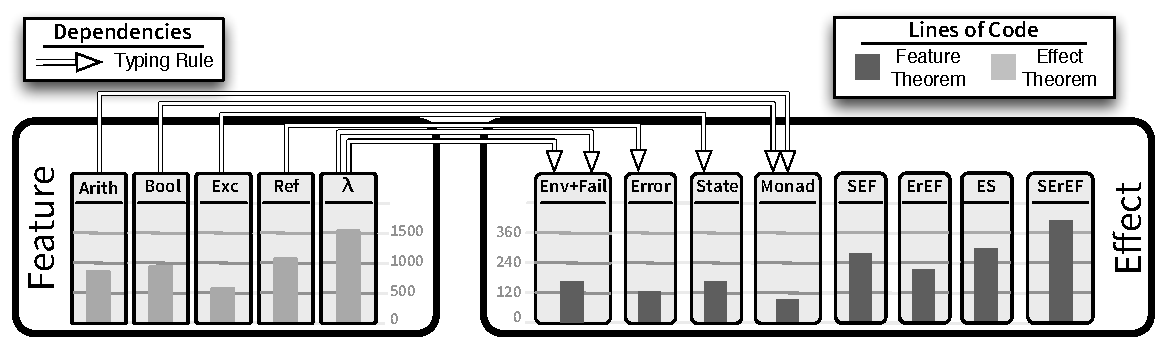
\includegraphics[scale = .85]{src/ModularEffects/CaseStudyFigure.pdf}
   }
  \end{center}
  \caption{Dependency and size information for the features and effects used in the case study.}
  \label{fig:codesize}
\end{figure*}

\section{Case Study}
\label{sec:CaseStudy}

As a demonstration of the \Name~framework, we have built a set of five
reusable language features and combined them to build a family of
languages which includes a mini-ML~\cite{clement86mini-ML} variant
with references and errors. The study includes pure boolean and
arithmetic features as well as effectful features for references,
errors and lambda abstractions.

The study builds twenty eight different combinations of the features which are
all possible combinations with at least one feature providing
values.\footnote{Also available at \url{http://www.cs.utexas.edu/~bendy/3MT}}
Figure~\ref{fig:MiniMLSyntax} presents the syntax of the expressions,
values, and types provided; each line is annotated with the feature
that provides that set of definitions.

Four kinds of feature interactions appear in the case study.

\begin{itemize}

\item The PHOAS representation of binders requires an auxiliary
equivalence relation, the details of which are covered in the MTC
paper~\cite{mtc}. The soundness proofs of language theorems for
languages which include binders proceed by induction over this
equivalence relation instead of expressions. The reusable feature
theorems of other features need to be lifted to this equivalence
relation.

\item The effect theorems that feature an environment
typing $\Sigma$, such as those for state or environment, need a weakening sublemma
which
states
that each well-formed value under
$\Sigma$ is also well-formed under a conservative extension:
\[\Sigma \vdash v ~:~ t  \\ \rightarrow \\
  \Sigma' \supseteq \Sigma \\ \rightarrow \\
  \Sigma' \vdash v ~:~ t \]
\item Inversion lemmas for the well-formed value relation as in the
proof of \ref{thm:FSound} for the boolean feature in
Section \ref{sec:Thm+Reuse} are proven by induction over the
relation.

%% \item The sublemmas of reusable feature theorems for properties such as
%% \textsc{WFM-If-Vc} are
%% proven by induction over the extensible typing relation. When effectful
%% features introduce new judgements to the relation, these new
%% judgements must have proof algebra instances for the sublemmas.

\end{itemize}


The proofs of the first and second kind of feature interactions are
straightforward; the inversion lemmas of the third kind can be
dispatched by tactics hooked into the type class inference algorithm.
%% The last kind of interactions require more work and comprise the
%% biggest part of the code dealing with feature interactions.
%%
%% The presented typing rules for effects satisfy the \textsc{WFM-Bind}
%% property; as previously discussed, it can be used cut down on feature
%% interactions. The lambda feature uses \textsc{WFM-Bind} in its proof
%% of \ref{thm:FSound} instead of targeted sublemmas. The following table
%% shows the number of sublemmas used by the reusable feature theorems,
%% highlighting that the \textsc{WFM-Bind} property provides significantly
%% more convenience despite its stronger assumptions.


The framework itself consists of about 4,400 LoC of which about 2,000
LoC comprise the implementation of the monad transformers and their
algebraic laws. The size in LoC of the implementation of semantic
evaluation and typing functions and the reusable feature theorem for
each language feature is given in the left box in Figure
\ref{fig:codesize}. The right box lists the sizes of the effect
theorems. Each language needs on average 110 LoC to assemble its
semantic functions and soundness proofs from those of its features and
the effect theorem for its set of effects.


\begin{figure}[t]
  \begin{center}
    \begin{minipage}{\columnwidth}
      \begin{center}
        \fbox{
        \hspace{-.3cm}
          \begin{tabular}{r@{~}c@{~}lr}
            {\tt e} & ::= & {\tt $\mathbb{N}$ $|$ e + e} & \textit{Arith}\\
            & $|$ &  {\tt $\mathbb{B}$ $|$ {\bf if} e {\bf then} e {\bf else} e} & \textit{Bool} \\
           %% & $|$ & {\tt {\bf case} e {\bf of \{ z} $\Rightarrow$ e $\mathbf{;}$ {\bf S} n $\Rightarrow$ e\}} & \textit{NatCase}\\
            & $|$ & {\tt {\bf lam} x : T.e $|$ e e $|$ x} & \textit{Lambda}\\
            & $|$ & {\tt {\bf ref} e $|$ !e $|$ e:=e} & \textit{References}\\
            & $|$ & {\tt {\bf try} e {\bf with} e} $|$ {\bf error} & \textit{Errors}\\
           %%  & $|$ & {\tt {\bf fix} x : T.e} & \textit{Recursion}\\
          \end{tabular}
        }
      \end{center}
    \end{minipage}
    \begin{minipage}{\columnwidth}
      \hspace{-.3cm}
    \begin{tabular}{cc}
      \begin{minipage}{.48\columnwidth}
        \fbox{
        \hspace{-.3cm}
          \begin{tabular}{r@{~}c@{~}lr}
            {\tt V} & ::= & {\tt $\mathbb{N}$} & \textit{Arith}\\
            & $|$ &  {\tt $\mathbb{B}$} & \textit{Bool} \\
            & $|$ & {\tt {\bf clos} e $\mathtt{\overline{V}}$} & \textit{Lambda}\\
            & $|$ & {\tt {\bf loc} $\mathbb{N}$} & \textit{References}\\
          \end{tabular}
        }
      \end{minipage} &
      \begin{minipage}{.38\columnwidth}
        \hspace{-.3cm}
        \fbox{
        \hspace{-.3cm}
          \begin{tabular}{r@{~}c@{~}lr}
            {\tt T} & ::= & {\tt \bf Nat} & \textit{Arith}\\
            & $|$ &  {\tt \bf Bool} & \textit{Bool} \\
            & $|$ & {\tt T $\rightarrow$ T} & \textit{Lambda}\\
            & $|$ & {\tt {\bf Ref} T} & \textit{References}\\
          \end{tabular}
        }
      \end{minipage}
    \end{tabular}
    \end{minipage}
  \end{center}
  \caption{mini-ML expressions, values, and types}
  \label{fig:MiniMLSyntax}
\end{figure}


%% \begin{center}
%%   \fbox{
%%   \hspace{-.3cm}
%%     \begin{tabular}{ c c c c c }
%%       \textit{Arith} & \textit{Bool} & \textit{Errors} & \textit{References} & \textit{Lambda} \\
%%       2 & 3 & 0 & 4 & 0 \\
%%     \end{tabular}
%%   }
%% \end{center}
%% Each sublemma of the above table requires on average 50 LoC per effect.

%% ODER: format ==         = "\mathrel{==}"
%% ODER: format /=         = "\neq "
%
%
\makeatletter
\@ifundefined{lhs2tex.lhs2tex.sty.read}%
  {\@namedef{lhs2tex.lhs2tex.sty.read}{}%
   \newcommand\SkipToFmtEnd{}%
   \newcommand\EndFmtInput{}%
   \long\def\SkipToFmtEnd#1\EndFmtInput{}%
  }\SkipToFmtEnd

\newcommand\ReadOnlyOnce[1]{\@ifundefined{#1}{\@namedef{#1}{}}\SkipToFmtEnd}
\usepackage{amstext}
\usepackage{amssymb}
\usepackage{stmaryrd}
\DeclareFontFamily{OT1}{cmtex}{}
\DeclareFontShape{OT1}{cmtex}{m}{n}
  {<5><6><7><8>cmtex8
   <9>cmtex9
   <10><10.95><12><14.4><17.28><20.74><24.88>cmtex10}{}
\DeclareFontShape{OT1}{cmtex}{m}{it}
  {<-> ssub * cmtt/m/it}{}
\newcommand{\texfamily}{\fontfamily{cmtex}\selectfont}
\DeclareFontShape{OT1}{cmtt}{bx}{n}
  {<5><6><7><8>cmtt8
   <9>cmbtt9
   <10><10.95><12><14.4><17.28><20.74><24.88>cmbtt10}{}
\DeclareFontShape{OT1}{cmtex}{bx}{n}
  {<-> ssub * cmtt/bx/n}{}
\newcommand{\tex}[1]{\text{\texfamily#1}}	% NEU

\newcommand{\Sp}{\hskip.33334em\relax}


\newcommand{\Conid}[1]{\mathit{#1}}
\newcommand{\Varid}[1]{\mathit{#1}}
\newcommand{\anonymous}{\kern0.06em \vbox{\hrule\@width.5em}}
\newcommand{\plus}{\mathbin{+\!\!\!+}}
\newcommand{\bind}{\mathbin{>\!\!\!>\mkern-6.7mu=}}
\newcommand{\rbind}{\mathbin{=\mkern-6.7mu<\!\!\!<}}% suggested by Neil Mitchell
\newcommand{\sequ}{\mathbin{>\!\!\!>}}
\renewcommand{\leq}{\leqslant}
\renewcommand{\geq}{\geqslant}
\usepackage{polytable}

%mathindent has to be defined
\@ifundefined{mathindent}%
  {\newdimen\mathindent\mathindent\leftmargini}%
  {}%

\def\resethooks{%
  \global\let\SaveRestoreHook\empty
  \global\let\ColumnHook\empty}
\newcommand*{\savecolumns}[1][default]%
  {\g@addto@macro\SaveRestoreHook{\savecolumns[#1]}}
\newcommand*{\restorecolumns}[1][default]%
  {\g@addto@macro\SaveRestoreHook{\restorecolumns[#1]}}
\newcommand*{\aligncolumn}[2]%
  {\g@addto@macro\ColumnHook{\column{#1}{#2}}}

\resethooks

\newcommand{\onelinecommentchars}{\quad-{}- }
\newcommand{\commentbeginchars}{\enskip\{-}
\newcommand{\commentendchars}{-\}\enskip}

\newcommand{\visiblecomments}{%
  \let\onelinecomment=\onelinecommentchars
  \let\commentbegin=\commentbeginchars
  \let\commentend=\commentendchars}

\newcommand{\invisiblecomments}{%
  \let\onelinecomment=\empty
  \let\commentbegin=\empty
  \let\commentend=\empty}

\visiblecomments

\newlength{\blanklineskip}
\setlength{\blanklineskip}{0.66084ex}

\newcommand{\hsindent}[1]{\quad}% default is fixed indentation
\let\hspre\empty
\let\hspost\empty
\newcommand{\NB}{\textbf{NB}}
\newcommand{\Todo}[1]{$\langle$\textbf{To do:}~#1$\rangle$}

\EndFmtInput
\makeatother
%
%
%
%
%
%
% This package provides two environments suitable to take the place
% of hscode, called "plainhscode" and "arrayhscode". 
%
% The plain environment surrounds each code block by vertical space,
% and it uses \abovedisplayskip and \belowdisplayskip to get spacing
% similar to formulas. Note that if these dimensions are changed,
% the spacing around displayed math formulas changes as well.
% All code is indented using \leftskip.
%
% Changed 19.08.2004 to reflect changes in colorcode. Should work with
% CodeGroup.sty.
%
\ReadOnlyOnce{polycode.fmt}%
\makeatletter

\newcommand{\hsnewpar}[1]%
  {{\parskip=0pt\parindent=0pt\par\vskip #1\noindent}}

% can be used, for instance, to redefine the code size, by setting the
% command to \small or something alike
\newcommand{\hscodestyle}{}

% The command \sethscode can be used to switch the code formatting
% behaviour by mapping the hscode environment in the subst directive
% to a new LaTeX environment.

\newcommand{\sethscode}[1]%
  {\expandafter\let\expandafter\hscode\csname #1\endcsname
   \expandafter\let\expandafter\endhscode\csname end#1\endcsname}

% "compatibility" mode restores the non-polycode.fmt layout.

\newenvironment{compathscode}%
  {\par\noindent
   \advance\leftskip\mathindent
   \hscodestyle
   \let\\=\@normalcr
   \let\hspre\(\let\hspost\)%
   \pboxed}%
  {\endpboxed\)%
   \par\noindent
   \ignorespacesafterend}

\newcommand{\compaths}{\sethscode{compathscode}}

% "plain" mode is the proposed default.
% It should now work with \centering.
% This required some changes. The old version
% is still available for reference as oldplainhscode.

\newenvironment{plainhscode}%
  {\hsnewpar\abovedisplayskip
   \advance\leftskip\mathindent
   \hscodestyle
   \let\hspre\(\let\hspost\)%
   \pboxed}%
  {\endpboxed%
   \hsnewpar\belowdisplayskip
   \ignorespacesafterend}

\newenvironment{oldplainhscode}%
  {\hsnewpar\abovedisplayskip
   \advance\leftskip\mathindent
   \hscodestyle
   \let\\=\@normalcr
   \(\pboxed}%
  {\endpboxed\)%
   \hsnewpar\belowdisplayskip
   \ignorespacesafterend}

% Here, we make plainhscode the default environment.

\newcommand{\plainhs}{\sethscode{plainhscode}}
\newcommand{\oldplainhs}{\sethscode{oldplainhscode}}
\plainhs

% The arrayhscode is like plain, but makes use of polytable's
% parray environment which disallows page breaks in code blocks.

\newenvironment{arrayhscode}%
  {\hsnewpar\abovedisplayskip
   \advance\leftskip\mathindent
   \hscodestyle
   \let\\=\@normalcr
   \(\parray}%
  {\endparray\)%
   \hsnewpar\belowdisplayskip
   \ignorespacesafterend}

\newcommand{\arrayhs}{\sethscode{arrayhscode}}

% The mathhscode environment also makes use of polytable's parray 
% environment. It is supposed to be used only inside math mode 
% (I used it to typeset the type rules in my thesis).

\newenvironment{mathhscode}%
  {\parray}{\endparray}

\newcommand{\mathhs}{\sethscode{mathhscode}}

% texths is similar to mathhs, but works in text mode.

\newenvironment{texthscode}%
  {\(\parray}{\endparray\)}

\newcommand{\texths}{\sethscode{texthscode}}

% The framed environment places code in a framed box.

\def\codeframewidth{\arrayrulewidth}
\RequirePackage{calc}

\newenvironment{framedhscode}%
  {\parskip=\abovedisplayskip\par\noindent
   \hscodestyle
   \arrayrulewidth=\codeframewidth
   \tabular{@{}|p{\linewidth-2\arraycolsep-2\arrayrulewidth-2pt}|@{}}%
   \hline\framedhslinecorrect\\{-1.5ex}%
   \let\endoflinesave=\\
   \let\\=\@normalcr
   \(\pboxed}%
  {\endpboxed\)%
   \framedhslinecorrect\endoflinesave{.5ex}\hline
   \endtabular
   \parskip=\belowdisplayskip\par\noindent
   \ignorespacesafterend}

\newcommand{\framedhslinecorrect}[2]%
  {#1[#2]}

\newcommand{\framedhs}{\sethscode{framedhscode}}

% The inlinehscode environment is an experimental environment
% that can be used to typeset displayed code inline.

\newenvironment{inlinehscode}%
  {\(\def\column##1##2{}%
   \let\>\undefined\let\<\undefined\let\\\undefined
   \newcommand\>[1][]{}\newcommand\<[1][]{}\newcommand\\[1][]{}%
   \def\fromto##1##2##3{##3}%
   \def\nextline{}}{\) }%

\newcommand{\inlinehs}{\sethscode{inlinehscode}}

% The joincode environment is a separate environment that
% can be used to surround and thereby connect multiple code
% blocks.

\newenvironment{joincode}%
  {\let\orighscode=\hscode
   \let\origendhscode=\endhscode
   \def\endhscode{\def\hscode{\endgroup\def\@currenvir{hscode}\\}\begingroup}
   %\let\SaveRestoreHook=\empty
   %\let\ColumnHook=\empty
   %\let\resethooks=\empty
   \orighscode\def\hscode{\endgroup\def\@currenvir{hscode}}}%
  {\origendhscode
   \global\let\hscode=\orighscode
   \global\let\endhscode=\origendhscode}%

\makeatother
\EndFmtInput
%
%
%
% First, let's redefine the forall, and the dot.
%
%
% This is made in such a way that after a forall, the next
% dot will be printed as a period, otherwise the formatting
% of `comp_` is used. By redefining `comp_`, as suitable
% composition operator can be chosen. Similarly, period_
% is used for the period.
%
\ReadOnlyOnce{forall.fmt}%
\makeatletter

% The HaskellResetHook is a list to which things can
% be added that reset the Haskell state to the beginning.
% This is to recover from states where the hacked intelligence
% is not sufficient.

\let\HaskellResetHook\empty
\newcommand*{\AtHaskellReset}[1]{%
  \g@addto@macro\HaskellResetHook{#1}}
\newcommand*{\HaskellReset}{\HaskellResetHook}

\global\let\hsforallread\empty

\newcommand\hsforall{\global\let\hsdot=\hsperiodonce}
\newcommand*\hsperiodonce[2]{#2\global\let\hsdot=\hscompose}
\newcommand*\hscompose[2]{#1}

\AtHaskellReset{\global\let\hsdot=\hscompose}

% In the beginning, we should reset Haskell once.
\HaskellReset

\makeatother
\EndFmtInput

% format runC         = "run\mathbb{C}_{\scalebox{0.6}{T}}"
% format C            = "\mathbb{C}_{\scalebox{0.6}{T}}"
%%format R            = "\mathbb{R}_{\scalebox{0.6}{T}}"


\section{Related and Future Work}

\paragraph{DGP in proof-assistants}

Datatype-generic programming started out as a form of language
extension such as PolyP \cite{jansson:polyp} or Generic Haskell
\cite{loh:dsgh}. Yet Haskell has turned out to be powerful enough to
implement datatype-generic programming in the language itself and over
the time a vast number of DGP libraries for Haskell have been proposed
\cite{cheney:ligd,syb,emgm,multirec,instantgenerics,uniplate,genericderiving}. Compared
with a language extension, a library is much easier to develop and
maintain.

Using the flexibility of dependent-types there are multiple proposals
for performing datatype-generic programming in proof assistants
\cite{dgpcoq,altenkirch:gpwdtp,benke:universes,loh:gpif,indexedcontainers}. This
setting not only allows the implementation of generic functions, but
also of generic proofs. The approaches vary in terms of how strictly
they follow the positivity or termination restrictions imposed by the
proof assistant. Some circumvent the type-checker at various points to
simplify the development or presentation while others put more effort
in convincing the type-checker and termination checker of the validity
\cite{ertt}. However, in all of the proposals there does not seem to
be any fundamental problem caused by the restrictions.


\paragraph{DGP for modular proofs}

Modularly composing semantics and proofs about the semantics has also
been addressed by \cite{schwaab:mtp} in the context of programming
language meta-theory. They perform their development in Agda and
similar to our approach they also use a universe approach based on
polynomial functors to represent modular datatypes. They split
relations for small-step operational semantics and well-typing on a
feature basis. However, the final fixed points are constructed manually
instead of having a generic representation of inductive families.

Using Coq's type classes both MTC and our approach also allow for more
automation in the final composition of datatypes, functions and
proofs. Agda features instance arguments that can be used to replace
type classes in various cases. However, the current implementation
does not perform recursive resolution and as a result Agda does not
support automation of the composition to the extent that is needed for
DTC-like approaches.


\paragraph{Combining different DGP approaches}

We have shown an embedding of the universe of polynomial functors into
the universe of containers. Similar inclusions between universes have
been done in the literature \cite{morris:cspf}. Magalh\~aes and L\"oh
\cite{jpm:fcadgp} have ported several popular DGP approaches from
Haskell to Agda and performed a formal comparison by proving inclusion
relations between the approaches.

DGP approaches differ in terms of the class of datatypes they capture and the
set of generic functions that can be implemented for them. Generic functions
can be transported from a universe into a sub-universe. However, we are not
aware of any DGP library with a systematic treatment of universes where each generic
function is defined on the most general universe that supports that function.


\paragraph{DGP for abstract syntax}

We have shown how to obtain more reuse by complementing modular
definitions with a generic equality function and generic proofs of its
properties. Of course more generic functionality like traversals,
pretty-printing, parsing etc. can be covered by means of
datatype-generic programming.

One very interesting idea is to use datatype-generic programming to
handle variable binding \cite{cheney:synp,unbound}. Variable
binding is an ubiquitous aspect of programming languages. Moreover, a
lot of functionality like variable substitutions and free variable
calculations is defined for many languages. Licata and Harper
\cite{licata:ubc} and Keuchel and Jeuring \cite{sk:gcasr} define
universes for datatypes with binding in Agda. Lee et al.~\cite{gmeta}
develop a framework for first-order representations of variable
binding in Coq that is based on the universe of regular tree types
\cite{ertt} and that provides many of the so-called
\emph{infrastructure lemmas} required when mechanizing programming
language meta-theory.

An interesting direction for future work is to extend these approaches
to capture variable binding in the indices of relations on abstract
syntax and use this as the underlying representation of extensible
datatypes and extensible logical relations and thereby complementing
modular functions with generic proofs about variable binding.


\paragraph{Automatic derivation of instances}

Most, if not all, generic programming libraries in Haskell use Template
Haskell to derive the generic representation of user-defined types and
to derive the conversion functions between them.

The GMeta \cite{gmeta} framework includes a standalone tool that also
performs this derivation for Coq. Similarly we also like to be able
to derive instances for the \ensuremath{\Conid{Container}} and \ensuremath{\Conid{Polynomial}} classes
automatically.


Formally mechanizing proofs can be very tedious and the amount of work
required for larger developments is excruciating. Meta-Theory \`a la Carte
is a framework for modular reusable components for use in
mechanizations. It builds on the Datatypes \`a la Carte approach to solve
an extended version of the expression problem. MTC allows modular
definitions of datatypes, semantic functions and logical relations and
furthermore modular inductive proofs.

MTC uses extensible Church-encodings to overcome conservative restrictions
imposed by the Coq proof-assistant. This approach has shortcomings
in terms of confidence in the definitions and in terms of usability. This
paper addresses these shortcomings by using datatype-generic
programming techniques to replace Church-encodings as the underlying representation
of type-level fixed points. Our approach avoids impredicativity, adequately
encodes fixed points and leads to stronger induction principles by
exploiting DGP approaches that capture only strictly-positive functors.

Working with generic structure representation has the added benefit that
we can implement generic functions like equality and generic proofs once and for all.


\chapter{Modular Monadic Effects}\label{ch:modmoneff}
{ % STLCBOOL SCOPE

\newcommand{\stlcbool}{\ensuremath{\lambda_{\mathbb{B}}}\xspace}
\newcommand{\bool}{\text{bool}}
\newcommand{\true}{\textbf{true}\xspace}
\newcommand{\false}{\textbf{false}\xspace}
\newcommand{\ite}[3]{\textbf{if}~{#1}~\textbf{then}~{#2}~\textbf{else}~{#3}}
\newcommand{\typing}[3]{{#1} \vdash {#2} : {#3}}
\renewcommand{\eval}[2]{{#1} \longrightarrow {#2}}
\newcommand{\evals}[2]{{#1} \longrightarrow^* {#2}}

\chapter{Introduction}

The concept of programming can be defined as communicating how to perform tasks
to a computer. An increasing number of fields such as biology, engineering,
physics, psychology and sociology rely on programming. Programming is not
limited to sciences. The ubiquity of computers and the pervasive use of software
in our society indirectly depend on programming and programmers.  However,
software is notoriously unreliable. Given the extent of our dependence on
software this is all the more detrimental and costly.

In order to improve upon this situation we need to meliorate the process of
programming itself.
\begin{itemize}
\item 'Programming languages' are the tools/methods for programming
\item The minimum requirement is that a program does what it's intended to do.
\end{itemize}

For a programmer it is essential that she can validate that a program implements
exactly the intended task which is usually achieved by reasoning with the
\emph{expected behaviour} of a program.

But how is the behaviour of programming constructs defined, or more generally,
how are programming languages defined? The majority of programming languages
start with a reference implementation that effectively defines the language.
% Examples of languages that are (still) defined this way include Perl -
% Perl~5~\cite{perllanguage} and Python~\cite{pythonlanguage}.

After widespread use, a language may go through a standardization process:
multiple stakeholders develop a common language specification.
% , e.g. PHP was standardized in 2014~\cite{phpspec}.
Another approach is develop specifications together with a reference
implementation. These two approaches are not mutually exclusive: languages with
an existing specification are extended in tandem with implementations.

Such a language specification allows a programmer to resolve ambiguities when
reasoning about her programs independent of a particular implementation. It also
enables us to switch between implementations.

Programming language theory is a branch of computer science that deals with
language specifications, design, implementation, and in particular also
meta-theoretical analysis of programming languages, their semantics and related
systems like type-systems. When developing new languages or language features we
want to make sure that the design is coherent and fulfills the expectations of
users.

The programmer is often given useful safety guarantees for this programs. For
instance, many modern programming language provide garbage collection
facilities. Yet we want our programs to be memory safe, i.e. they do not access
memory that has been freed or that has not yet been initialized. Another safety
property is type-safety, i.e. the absence of dynamic type errors during
execution. These guarantees are usually provided for all programs written in a
language or a specific subset of programs, e.g. all type-checked programs. In a
meta-theoretical analysis we want to make sure that these are indeed valid
guarantees.

The meta-theory of programming language semantics and type-systems is highly
complex due to the management of many details and edge cases. As such, it is
prone to subtle errors that can invalidate large amounts of work.

For example, the Java programming language was long believed to be type-safe
\footnote{Except for some deliberate defects like the co-variance of arrays.}
but the addition of Generics made Java's type system in fact unsound
\cite{amin2016java}. Another problem concerns the type-checking of Java
programs. Generics made type-checking an undecidable property of
programs~\cite{grigore2017}. Decidability of type-checking does not have an
impact on properties that we get for type-checked programs, but for example it
opens up attack vectors on (web) services that deal with Java code because the
type-checker may run forever.

To increase the confidence in the correctness of formal meta-theory, techniques
for formalization in proof-assistants, also known as mechanization, have
received much attention. These systems allow us to state mathematical statements
and proofs for them and let the machine check that these are in fact valid
proofs. However, the high development cost of mechanizations continues to
prevent their widespread use. This leads us to the research question that this
thesis tries to answer:

\begin{center}
  \begin{minipage}{0.8\columnwidth}
    How can we reduce the costs of mechanizing formal meta-theory of programming
    languages?
  \end{minipage}
\end{center}

\begin{itemize}
\item Current methodology.
\item Why is the current methodology costly?
\item Give an idea of the relative effort.
\item What is the approach answer of this thesis?

  Increase reusability of code. Two strands: Modularity / Genericity.
\end{itemize}




The remainder of this chapter will give a more detailed introduction to the
relevant disciplines of specification, analysis and mechanization of programming
languages similar to what can be found in introductory textbooks such as
\cite{tapl}.

%% %-------------------------------------------------------------------------------
%% \section{Mechanization}
%% Mechanizing formal meta-theory in proof-assistants is crucial, both for the
%% increased confidence in complex designs and as a basis for technologies such as
%% proof-carrying code.  Formal reasoning in proof-assistants, also known as
%% mechanization, has high development costs.
%%

%% \begin{itemize}
%% \item
%%   Derive properties for all programs written in a language, like memory-safety,
%%   type-safety, resources-safety, termination, absence of deadlocks, race
%%   conditions and starvation.
%%
%% \item
%%   Prove correctness (preservation of semantics) of program analyses or compiler
%%   transformations.
%%
%%   by looking formally on the semantics, type systems and implementations like
%%   compilers or interpreters.
%% \end{itemize}

%-------------------------------------------------------------------------------
\section{Specifications}\label{sec:intro:specification}

%% Standardization and functional or program specifications are an essential
%% methodology in systems engineering and software development. It serves as the
%% baseline for correctness of implementations. Furthermore, multiple
%% implementations that are correct with respect to a common specification are
%% inter-operable or compatible to a certain extent. The precise meaning depends
%% on the context and the requirements.
%%
%% For programming languages for example, we want to guarantee that the same
%% program is executable by different implementations and performs the same
%% tasks.  This does for example also ensures that program analyses and program
%% transformations, e.g. for optimization, can be developed independent of a
%% particular implementation and adopted by multiple implementations.
%%
%% In this thesis, we are interested in programming languages themselves and not
%% so much interested in their implementations. Hence, a specification of a
%% application binary interface, for example, to achieve binary compatibility of
%% modules compiled by different compilers is beyond the scope of this thesis.

Specifications differ in the detail and precision they describe systems.
Industrial specifications of major programming languages are usually written in
natural language and are detailed to cover every aspect of the languages. The
use of natural language leaves opportunities for ambiguity, but disregarding
this problem, elaborate industrial specifications provide a good reference point
for language users and implementors. However, for meta-theoretical analyses more
rigorous specifications are necessary.

We will use \emph{formal specifications} and a mathematical language to
describe programming languages. This gives use the necessary precision and
avoids the ambiguities of natural languages. This section explains necessary
fundamental concepts for the formal specification of programming languages by
example of a small language \stlcbool: a simply-typed lambda calculus with
booleans. We specify the \emph{abstract syntax}, \emph{static type system} and
\emph{evaluation} of \stlcbool using inductive definitions. Along the way, we
define the terminology and notational conventions and make their meaning
precise.

%-------------------------------------------------------------------------------
\subsection{Syntax}\label{ssec:intro:syntax}

\begin{figure}[t]
  \centering
  \fbox{
    \begin{minipage}{\columnwidth}
    \begin{tabular}{lcll}
      $x,y$           & ::=    &                            & term variable    \\
      $\tau,\sigma$   & ::=    &                            & type             \\
                      & $\mid$ & $\tau \to \tau$            & function type    \\
                      & $\mid$ & $\bool$                    & boolean type     \\
      $e$             & ::=    &                            & term             \\
                      & $\mid$ & $\true$                    & true constant    \\
                      & $\mid$ & $\false$                   & false constant   \\
                      & $\mid$ & $\ite{e}{e}{e}$            & conditional      \\
                      & $\mid$ & $x$                        & term variable    \\
                      & $\mid$ & $\lambda x:\tau.e$         & term abstraction \\
                      & $\mid$ & $e~e$                      & application      \\
      $v$             & ::=    &                            & term             \\
                      & $\mid$ & $\true$                    & true constant    \\
                      & $\mid$ & $\false$                   & false constant   \\
                      & $\mid$ & $\lambda x:\tau.e$         & term abstraction \\
      $\Gamma$        & ::=    &                            & type context     \\
                      & $\mid$ & $\epsilon$                 & empty context    \\
                      & $\mid$ & $\Gamma, x:\tau$           & term binding     \\
    \end{tabular}
    \end{minipage}
  }
  \caption{\stlcbool syntax}
  \label{fig:intro:stlcboolsyntax}
\end{figure}

The syntax of \stlcbool is given in Figure \ref{fig:intro:stlcboolsyntax}. We
use a convention that is close to standard \textsc{EBnf} grammars. Elided in the
grammar are syntactic constructs like parentheses. We use parentheses freely to
resolve ambiguities in terms even if the grammar does not define them. Any
implementation that deals with the concrete syntax of a programming language has
of course to be more rigorous.

The grammar in Figure \ref{fig:intro:stlcboolsyntax} defines several
\emph{syntactic sorts} for \stlcbool. The \emph{meta-variable} $e$ stands for
expressions of \stlcbool of which there are 6 different kinds. An expression can
either be a boolean constant $\true$ or $\false$, a conditional form
$\ite{e_c}{e_t}{e_e}$, an \emph{object-language variable} (represented by the
meta-variable $x$), the definition of a function as a \textlambda-abstraction
$(\lambda x:\tau.e)$ or the application of an expression $e_1$ to another
expression $e_2$. Of course we only want to apply expressions $e_1$ that
represent functions: either by being a \textlambda-abstraction or evaluating to
one. Applying any \emph{value} other than a \textlambda-abstraction is a
\emph{type error}. We make this more precise below and come back to it it
Section \ref{sec:intro:typesafety} on analysis.

The grammar also includes the meta-variable $\tau$ that describes the types of
\stlcbool. Each \textlambda-abstraction contains a \emph{type annotation} $\tau$
for the argument variable $x$. The denotation is that the function represented
by the \textlambda-abstraction expects a value of type $\tau$ when it is
applied. We discuss types and typing contexts $\Gamma$ in more detail in Section
\ref{ssec:intro:typing} which deals with static typing.


%-------------------------------------------------------------------------------
\subsection{Semantics}\label{ssec:intro:semantics}

We have defined the syntax of \stlcbool expressions and can now turn towards
defining their meaning. There are multiple established ways to define semantics
of programming language. We can coarsely classify the approaches into three
different groups:

\begin{enumerate}
\item Operational Semantics

  Operational semantics defines the meaning of programs by specifying their
  execution in a state transition system. A \emph{state transition function} or
  a \emph{state transition relation} on the terms of the programming language
  defines the possible execution steps. The program is part of the state. For
  small languages the entire state might consist of only the program. After
  taking a step we are left with an updated state that includes a residual
  program.

  %% We can then define the meaning of programs to be the execution process on
  %% the abstract machine.


\item Denotational Semantics

  Denotational semantics defines the meaning of programs in terms of collection
  of \emph{mathematical semantic domains} that can include numbers, sets or
  functions. An \emph{interpretation function} maps program terms into these
  domains. This function is generally compositional in the syntax which
  is beneficial for modularity.

  Usually, the semantic domain has an established \emph{formal theory}. The
  theorems of the domain give rise to reasoning laws for programs. Furthermore,
  we can also derive properties of programming languages from properties of the
  collection of semantic domains.

\item Axiomatic Semantics

  Instead of deriving laws for programs from their execution behaviour or
  denotation we can also axiomatically assume these laws. This is known as an
  axiomatic semantics.

  This gives us immediately the means for reasoning about programs. Furthermore,
  we can derive a denotational semantics for the language by constructing a
  model that satisfies the chosen laws and derive properties for this model or
  even all models.

\end{enumerate}

These approaches have different trade-offs. Denotational and axiomatic semantics
immediately give us powerful mathematical tools to reason about programming
languages and their programs, but for larger languages the required technicality
and complexity makes it extremely difficult to even define a suitable semantics.

Operational semantics do not give us the same powerful mathematical reasoning
techniques and instead impose on us the laborious task to reason about programs
by observing their behaviour during execution. However, operational semantics
are simpler and easier to define than more abstract denotational or axiomatic
semantics. Moreover, they are much closer to actual implementations. Due to the
smaller gap, operational semantics make it easier to reason about the
correctness of implementations.

\begin{figure}[t]
  \centering
  \fbox{
    \begin{minipage}{\columnwidth}
      \framebox{\mbox{$\eval{e}{e}$}}\\
      \vspace{-5mm}
      \[ \begin{array}{c}
           \inferrule* [right=\textsc{EIfTrue},]
             {
             }
             {\eval{\ite{\true}{e_t}{e_e}}{e_t}
             } \\\\
           \inferrule* [right=\textsc{EIfFalse}]
             {
             }
             {\eval{\ite{\false}{e_t}{e_e}}{e_e}
             } \\\\
           \inferrule* [right=\textsc{EIf}]
             {\eval{e_c}{e_c'}
             }
             {\eval{\ite{e_c}{e_t}{e_e}}{\ite{e_c'}{e_t}{e_e}}
           } \\\\
           \inferrule* [right=\textsc{EAppAbs}]
             {
             }
             {\eval{(\lambda x:\tau.e_1)~e_2}{[x \mapsto e_2]e_1}
             } \\\\
           \inferrule* [right=\textsc{EApp}]
             {\eval{e_1}{e_2'}
             }
             {\eval{e_1~e_2}{e_1'~e_2}
             } \\\\
         \end{array}
       \]
    \end{minipage}
  }
  \caption{\stlcbool reduction rules}
  \label{fig:intro:stlcbooleval}
\end{figure}

For our \stlcbool language we define semantics using a \emph{small-step
  operational semantics}. This is also the approach used in Part \ref{part:gen}
of this thesis. Part \ref{part:mod} uses denotational semantics.

Figure \ref{fig:intro:stlcbooleval} gives the complete definition of the
operational semantics by means of an evaluation relation. The box in the upper
left corner \framebox{\mbox{$\eval{e_1}{e_2}$}} defines the shape and notation
that we use for the relation. In this case it is a binary relation between two
terms, which denotes that $e_1$ evaluates to $e_2$ in one step.

The remainder of the figure defines the relation using Gentzen-style inference
rules~\cite{gentzen1935}. In general, rules take the form
\[
  \inferrule* [right=\textsc{Name}]
    {J_1 \\ J_2 \\ \ldots \\ J_n
    }
    {J
    }
\]
where \textsc{Name} is an optional name for the rule that allows us to refer to
it. The meta-variable $J$ stands for judgements, which in our case are usually
mathematical statements in propositional or first-order logic. The judgements
$J_1, \ldots, J_n$ above the horizontal line are the premises of the rule, and
the judgement $J$ below the line is the conclusion. Rule without any premises
are also called \emph{axioms}. The conclusion will always involve the relation
that is being defined.

The single-step evaluation is defines using five rules. The two axioms
\textsc{EIfTrue} and \textsc{EIfFalse} show how to reduce an
\textbf{if}-expression in case the condition is either a \true or a \false
value. The case of a condition that is not yet fully evaluated is handled by
rule \textsc{EIf}. If the condition $e_c$ reduces to $e_c'$ in one step then we
can conclude the one step reduction
\[ \eval{\ite{e_c}{e_t}{e_e}}{\ite{e_c'}{e_t}{e_e}} \]

The last two rules cover the evaluation of \textlambda-terms. The rule
\textsc{EAppAbs} handles the case where the left-hand side of an application is
a \textlambda-term $(\lambda x:\tau.e_1)$. The residual program is the the body
$e_1$ of the function after substituting $e_2$ for $x$ which we write as
$[x \mapsto e_2]e_1$. The argument of the function does not have to be fully
evaluated, i.e. the rules encode a \emph{call-by-name} evaluation strategy. If
the left-hand side is not yet a \textlambda-term, we evaluate it first similarly
to \textsc{EIf}.

Note that this definition does not cover all the cases. In particular
the case of a \textlambda-term in the condition of an \textbf{if}-expression
\[ \ite{(\lambda x:\tau.e)}{e_t}{e_e} \]
\noindent and the cases of a boolean in the left-hand side of an application
\[ \true~e_1 \qquad \text{or} \qquad \false~e_2 \]
\noindent are not specified. Since no transition is defined and the execution
stopped without any \emph{meaningful result}, we also say that the evaluation
got stuck. In an implementation of the programming language, this corresponds to
an error that can happen during execution of a program. It's therefore also
called a \emph{(dynamic) type error}. Programmers want to detect potential
problems like that early in the development cycle and, if possible, at compile
time. This motivates the development of \emph{static type systems}.

%-------------------------------------------------------------------------------
\subsection{Typing}\label{ssec:intro:typing}

\begin{figure}[t]
  \centering
  \fbox{
    \begin{minipage}{\columnwidth}
      \framebox{\mbox{$\typing{\Gamma}{e}{\tau}$}}\\
      \vspace{-5mm}
      \[ \begin{array}{c}
           \inferrule* [right=\textsc{TTrue}]
             {
             }
             {\typing{\Gamma}{\true}{\bool}
             } \quad
           \inferrule* [right=\textsc{TFalse}]
             {
             }
             {\typing{\Gamma}{\false}{\bool}
             } \\\\
           \inferrule* [right=\textsc{TIf}]
             {\typing{\Gamma}{e_c}{\bool} \\
              \typing{\Gamma}{e_t}{\tau} \\
              \typing{\Gamma}{e_e}{\tau}
             }
             {\typing{\Gamma}{\ite{e_c}{e_t}{e_e}}{\tau}
             } \\\\
           \inferrule* [right=\textsc{TVar}]
             {x : \tau \in \Gamma
             }
             {\typing{\Gamma}{x}{\tau}
             } \quad
           \inferrule* [right=\textsc{TAbs}]
             {\typing{\Gamma,y:\sigma}{e}{\tau}
             }
             {\typing{\Gamma}{(\lambda y:\sigma. e)}{(\sigma\to\tau)}
             } \\\\
           \inferrule*[right=\textsc{TApp}]
             {\typing{\Gamma}{e_1}{\sigma \to \tau} \\
              \typing{\Gamma}{e_2}{\sigma}
             }
             {\typing{\Gamma}{e_1~e_2}{\tau}
             }
         \end{array}
       \]
    \end{minipage}
  }
  \caption{\stlcbool typing rules}
  \label{fig:intro:stlcbooltyping}
\end{figure}

A \emph{type system} is an assignment of types to expressions. Usually not all
expressions are typeable and un-typeable expressions are rejected. Also in some
languages there are expressions that can be assigned multiple, potentially
incomparable types. Both, the partiality and the ambiguity of types, suggests a
\emph{relational} rather than a \emph{functional} assignment. Such a relation is
defined in Figure \ref{fig:intro:stlcbooltyping}. It is a ternary relation
\framebox{\mbox{$\typing{\Gamma}{e}{\tau}$}} between a typing context $\Gamma$,
an expression $e$ and a type $\tau$.

The typing relation is defined using six rules. The two rules \textsc{TTrue} and
\textsc{TFalse} respectively state that the boolean constants $\true$ and
$\false$ have a boolean type. The rule \textsc{TIf} handles the case of an
\textbf{if}-expression. The three sub-expression position contain a
meta-variables $e_c$, $e_t$ and $e_e$. The premises require that the condition
$e_c$ has type boolean and the \textbf{then} and \textbf{else} branches have the
same type $\tau$. The rule then concludes that the entire \textbf{if}-expression
also has type $\tau$.

The three remaining rules deal with $\lambda$-abstractions. The typing context
$\Gamma$ is a list that associates term variables with types. In the case of a
variable, rule \textsc{TVar} looks up the corresponding type in $\Gamma$. Rule
\textsc{TAbs} checks the body of a $\lambda$-abstraction in the context
$(\Gamma,y:\sigma)$ which is the outside context $\Gamma$ extended with a pair
for the $lambda$-bound variable $y$. The type of the $\lambda$-abstraction is
the function type $(\sigma \to \tau)$ between the argument type $\sigma$ and the
type of the body $\tau$. Finally, rule \textsc{TApp} requires that the left
expressions of an application has a function type that is compatible with the
argument.

\paragraph{Example}
Consider the boolean negation function
\[
  \lambda y:\bool. \ite{y}{\false}{\true}
\]

This function sends booleans to booleans and should therefore have the type
$\bool\to\bool$. Giving the above typing relations, we can repeatedly apply the
rule to get a typing derivation for this. At each step only one possible rule
applies. We can arrange the rule applications in a so called \emph{derivation
  tree} that illustrates the whole derivation. Using the abbreviation
$\Gamma' := \Gamma, y:\bool$, we have the following tree:

\[
  \inferrule*
  { \inferrule*
    {
      \inferrule*{\;}{\typing{\Gamma'}{y}{\bool}} \\
      \inferrule*{\;}{\typing{\Gamma'}{\false}{\bool}} \\
      \inferrule*{\;}{\typing{\Gamma'}{\true}{\bool}} \\
    }
    {\typing{\Gamma'}{\ite{y}{\false}{\true}}{\bool}
    }
  }
  { \typing{\Gamma}{\lambda y:\bool. \ite{y}{\false}{\true}}{\bool \to \bool}
  }
\]


%-------------------------------------------------------------------------------
\section{Meta-Theoretical Analysis}\label{sec:intro:typesafety}

It is folklore in software development that bugs arise in both implementations
and in specifications. For instance, \cite{arts2015testing} describes a war
story on testing car software in which they found 227 bugs in the
\textsc{Autosar} specification (and in implementations).

To ensure that our languages are well-designed we want to establish
meta-theoretical properties that ensures that all the guarantees a user expects
are indeed valid. This needs a rigorous and formal analysis of the defined
semantics of a programming language. In this section we will look at the precise
definition of the type-safety language property, present methods for reasoning
about semantics and outline how these can be used to prove the type-safety
property for for our example calculus \stlcbool.

We previously characterized type-safety as the absence of type-errors during
execution. A type-error represents a state for which no further evaluation step
is defined and hence evaluation stopped.

\begin{defn}[Normal Form]
  An expression $e_1$ is a \emph{normal form} if no further execution step can be
  taken, i.e.
  \[ \forall e_2. \neg (\eval{e_1}{e_2}) \]
\end{defn}

A type-error however did not produce any \emph{meaningful result}. Let us define
what a meaningful result is. These are special expressions which are also called
values.

\begin{defn}[Value]
  Values are the subset of expressions that are defined by the following
  grammar:
  \begin{center}
    \begin{tabular}{lcll}
      $v$ & ::=    &                    & term             \\
          & $\mid$ & $\true$            & true constant    \\
          & $\mid$ & $\false$           & false constant   \\
          & $\mid$ & $\lambda x:\tau.e$ & term abstraction \\
    \end{tabular}
  \end{center}
\end{defn}

Expressions with type-errors are hence normal forms that are not values. We can
hence make \emph{the absence of type error} more precise by requiring that all
normal forms are already values.

\begin{thm}[Type-Safety]
  Let $\typing{\cdot}{e_1}{\tau}$. If $e_1$ evaluates to a normal form $e_2$
  then $e_2$ is a value.
\end{thm}

Note that this definition does not require the evaluation to terminate.  A
program that runs forever without a type-error is also considered type-safe.


\paragraph{Inductive Reasoning}
Figures \ref{fig:intro:stlcbooleval} and \ref{fig:intro:stlcbooltyping} define
evaluation and typing for \stlcbool. More precisely, our intention is to define
the \emph{smallest relation} that includes the presented rules. This gives rise
to a \emph{structural induction principle} for the relations. Put differently,
we can induct over the shape of derivation trees (or their size or height).

%% As an example consider the following determinacy theorem which states that
%% at each point there at most one possible successor state.
%% \begin{thm}[Determinacy]
%%   If $\eval{e_1}{e_2} \wedge \eval{e_1}{e_3}$ then $e_2 = e_3$.
%% \end{thm}


\begin{lem}[Progress]
  Let $\typing{\cdot}{e_1}{\tau}$. Either $e_1$ is a value or we can take another
  step, i.e.
  \[ \exists e_2. \eval{e_1}{e_2}. \]
\end{lem}


\begin{lem}[Preservation]
  If $\typing{\Gamma}{e_1}{\tau}$ and $\eval{e_1}{e_2}$ then $\typing{\Gamma}{e_2}{\tau}$.
\end{lem}




\section{Mechanization}

that he expects we need to

of languages on their own are not good enough to ensure a
good design.




The undecidability of type-checking Java~\cite{grigore2017} and the unsoundness
of its type system \cite{amin2016java} might be seen as bugs of the language
specification (but no formal specification of the complete Java language
exists).


A good approach is to develop software (and programming languages) in tandem
with an implementation and refine both. However, problems usually arise in
subtle edge cases that do not appear in normal program code that we write every
day and are easy to overlook in an





and such properties have only been established for subsets of the language such
as Featherweight Java \cite{igarashi2001featherweight}.

\begin{itemize}
\item
  Improving the correctness of C compilers is a worthy goal: C code is part of
  the trusted computing base for almost every modern computer system including
  mission-critical financial servers and life- critical pacemaker firmware.
\end{itemize}
From \cite{yang2011bugs}:

\blockquote{ The striking thing about our \textsc{CompCert} results is that the
  middle-end bugs we found in all other compilers are absent. As of early 2011,
  the under-development version of \textsc{CompCert} is the only compiler we
  have tested for which \textsc{Csmith} cannot find wrong-code errors. This is
  not for lack of trying: we have devoted about six CPU-years to the task. The
  apparent unbreakability of \textsc{CompCert} supports a strong argument that
  developing compiler optimizations within a proof framework, where safety
  checks are explicit and machine-checked, has tangible benefits for compiler
  users.}


%% The meta-theory of programming language semantics and type-systems is highly
%% complex due to the management of many details. Formal proofs are long and prone
%% to subtle errors that can invalidate large amounts of work. In order to
%% guarantee the correctness of formal meta-theory, techniques for mechanical
%% formalization in proof-assistants have received much attention in recent years.
%%
%% %-------------------------------------------------------------------------------
%% \section{Mechanization}
%% Mechanizing formal meta-theory in proof-assistants is crucial, both for the
%% increased confidence in complex designs and as a basis for technologies such as
%% proof-carrying code.  Formal reasoning in proof-assistants, also known as
%% mechanization, has high development costs.
%%
%% To lighten the burden of programming language mechanization, many
%% approaches have been developed that tackle the substantial boilerplate which
%% arises from variable binders. Unfortunately, the existing approaches are limited
%% in scope.
%% %% STEVEN: This is still valid, but I hope it's not misleading the reader into
%% %% thinking we deal with typing relations directly.
%% As a consequence, the human mechanizer is still unnecessarily burdened with
%% binder boilerplate and discouraged from taking on richer languages.
%%
%% This paper presents \Knot, a new approach that substantially extends the support
%% for binder boilerplate. \Knot is a highly expressive language for natural and
%% concise specification of syntax with binders. Its meta-theory constructively
%% guarantees the coverage of a considerable amount of binder boilerplate for
%% well-formed specifications, including that for well-scoping of terms and context
%% lookups. \Knot also comes with a code generator, \Needle, that specializes the
%% generic boilerplate for convenient embedding in \Coq and provides a tactic
%% library for automatically discharging proof obligations that frequently come up
%% in proofs of weakening and substitution lemmas of type-systems.
%%
%% Our evaluation shows, that Needle \& Knot significantly reduce the size of
%% language mechanizations (by 40\% in our case study). Moreover, as far as we
%% know, \Knot enables the most concise mechanization of the \POPLmark Challenge
%% (1a + 2a) and is two-thirds the size of the next smallest. Finally, \Knot allows
%% us to mechanize for instance dependently-typed languages, which is notoriously
%% challenging because of dependent contexts and mutually-recursive sorts with
%% variables.
%%
%% %-------------------------------------------------------------------------------
%% \section{Binding}
%%
%% To lighten the burden of programming language mechanization, many approaches
%% have been developed that tackle the substantial boilerplate which arises from
%% variable binders. Unfortunately, existing approaches for first-order
%% representations are limited to the boilerplate that concerns the syntax of
%% languages and do not tackle common boilerplate lemmas that arise for semantic
%% relations such as typing. Consequently, the human mechanizer is still burdened
%% with proving these substantial boilerplate lemmas manually.
%%
%% %% POPL 2014 Submission
%% %%
%% %%   A key concern in the mechanization of programming language metatheory is
%% %%   the representation of terms with variable binding. The properties of
%% %%   operations manipulating terms are notoriously burdensome to prove and the
%% %%   amount of work required to scale formalizations to realistic programming
%% %%   languages with rich binding forms is deemed infeasible. This is a pity,
%% %%   because we lose the practical benefits of mechanizing real programming
%% %%   languages.
%% %%
%% %%   We present a new solution to generically handle the boilerplate involved in
%% %%   mechanizations that scales to rich binding forms and advanced rules of
%% %%   scoping. We define a new specification language for abstract syntax with
%% %%   binding and implement a code generator that produces \Coq code for the
%% %%   representation of the abstract syntax, syntactic operations and proofs of
%% %%   their properties.
%% %%
%% %%   We illustrate how our approach removes the burden of variable binding
%% %%   boilerplate in the mechanization of realistic programming languages on a
%% %%   list of example specifications and a solution of the PoplMark challenge
%% %%   based on the generated code.

} % STLCBOOL SCOPE

\section{Overview}

\begin{center}
  \begin{minipage}{0.8\columnwidth}
    Keuchel, S., \& Schrijvers, T. (2013).
    \newblock Generic Datatypes à la Carte.
    \newblock In {\em Proceedings of the 9th ACM SIGPLAN workshop on Generic
      programming}, WGP ’13, pages 13-24. ACM.
  \end{minipage}
\end{center}

\begin{center}
  \begin{minipage}{0.8\columnwidth}
    Delaware, B., Keuchel, S., Schrijvers, T., and Oliveira,
    B. C. d.~S. (2013).
    \newblock Modular Monadic Meta-Theory.
    \newblock In {\em Proceedings of the 18th ACM SIGPLAN international
      conference on Functional programming}, ICFP '13, pages 319-330. ACM.
  \end{minipage}
\end{center}

\begin{center}
  \begin{minipage}{0.8\columnwidth}
    Keuchel, S. and Schrijvers, T. (2012).
    \newblock Modular Monadic Reasoning, a (Co-)Routine.
    \newblock Presented at \emph{the 24th Symposium on Implementation and
      Application of Functional Languages}, IFL '12.
  \end{minipage}
\end{center}


%%% Local Variables:
%%% mode: latex
%%% TeX-master: "../Main"
%%% End:

\input{src/ModEffects/Library}
\input{src/ModEffects/MonadicSemantics}
\input{src/ModEffects/MonadicTypeSafety}
\input{src/ModEffects/EffectLanguageTheorems}
%% ODER: format ==         = "\mathrel{==}"
%% ODER: format /=         = "\neq "
%
%
\makeatletter
\@ifundefined{lhs2tex.lhs2tex.sty.read}%
  {\@namedef{lhs2tex.lhs2tex.sty.read}{}%
   \newcommand\SkipToFmtEnd{}%
   \newcommand\EndFmtInput{}%
   \long\def\SkipToFmtEnd#1\EndFmtInput{}%
  }\SkipToFmtEnd

\newcommand\ReadOnlyOnce[1]{\@ifundefined{#1}{\@namedef{#1}{}}\SkipToFmtEnd}
\usepackage{amstext}
\usepackage{amssymb}
\usepackage{stmaryrd}
\DeclareFontFamily{OT1}{cmtex}{}
\DeclareFontShape{OT1}{cmtex}{m}{n}
  {<5><6><7><8>cmtex8
   <9>cmtex9
   <10><10.95><12><14.4><17.28><20.74><24.88>cmtex10}{}
\DeclareFontShape{OT1}{cmtex}{m}{it}
  {<-> ssub * cmtt/m/it}{}
\newcommand{\texfamily}{\fontfamily{cmtex}\selectfont}
\DeclareFontShape{OT1}{cmtt}{bx}{n}
  {<5><6><7><8>cmtt8
   <9>cmbtt9
   <10><10.95><12><14.4><17.28><20.74><24.88>cmbtt10}{}
\DeclareFontShape{OT1}{cmtex}{bx}{n}
  {<-> ssub * cmtt/bx/n}{}
\newcommand{\tex}[1]{\text{\texfamily#1}}	% NEU

\newcommand{\Sp}{\hskip.33334em\relax}


\newcommand{\Conid}[1]{\mathit{#1}}
\newcommand{\Varid}[1]{\mathit{#1}}
\newcommand{\anonymous}{\kern0.06em \vbox{\hrule\@width.5em}}
\newcommand{\plus}{\mathbin{+\!\!\!+}}
\newcommand{\bind}{\mathbin{>\!\!\!>\mkern-6.7mu=}}
\newcommand{\rbind}{\mathbin{=\mkern-6.7mu<\!\!\!<}}% suggested by Neil Mitchell
\newcommand{\sequ}{\mathbin{>\!\!\!>}}
\renewcommand{\leq}{\leqslant}
\renewcommand{\geq}{\geqslant}
\usepackage{polytable}

%mathindent has to be defined
\@ifundefined{mathindent}%
  {\newdimen\mathindent\mathindent\leftmargini}%
  {}%

\def\resethooks{%
  \global\let\SaveRestoreHook\empty
  \global\let\ColumnHook\empty}
\newcommand*{\savecolumns}[1][default]%
  {\g@addto@macro\SaveRestoreHook{\savecolumns[#1]}}
\newcommand*{\restorecolumns}[1][default]%
  {\g@addto@macro\SaveRestoreHook{\restorecolumns[#1]}}
\newcommand*{\aligncolumn}[2]%
  {\g@addto@macro\ColumnHook{\column{#1}{#2}}}

\resethooks

\newcommand{\onelinecommentchars}{\quad-{}- }
\newcommand{\commentbeginchars}{\enskip\{-}
\newcommand{\commentendchars}{-\}\enskip}

\newcommand{\visiblecomments}{%
  \let\onelinecomment=\onelinecommentchars
  \let\commentbegin=\commentbeginchars
  \let\commentend=\commentendchars}

\newcommand{\invisiblecomments}{%
  \let\onelinecomment=\empty
  \let\commentbegin=\empty
  \let\commentend=\empty}

\visiblecomments

\newlength{\blanklineskip}
\setlength{\blanklineskip}{0.66084ex}

\newcommand{\hsindent}[1]{\quad}% default is fixed indentation
\let\hspre\empty
\let\hspost\empty
\newcommand{\NB}{\textbf{NB}}
\newcommand{\Todo}[1]{$\langle$\textbf{To do:}~#1$\rangle$}

\EndFmtInput
\makeatother
%
%
%
%
%
%
% This package provides two environments suitable to take the place
% of hscode, called "plainhscode" and "arrayhscode". 
%
% The plain environment surrounds each code block by vertical space,
% and it uses \abovedisplayskip and \belowdisplayskip to get spacing
% similar to formulas. Note that if these dimensions are changed,
% the spacing around displayed math formulas changes as well.
% All code is indented using \leftskip.
%
% Changed 19.08.2004 to reflect changes in colorcode. Should work with
% CodeGroup.sty.
%
\ReadOnlyOnce{polycode.fmt}%
\makeatletter

\newcommand{\hsnewpar}[1]%
  {{\parskip=0pt\parindent=0pt\par\vskip #1\noindent}}

% can be used, for instance, to redefine the code size, by setting the
% command to \small or something alike
\newcommand{\hscodestyle}{}

% The command \sethscode can be used to switch the code formatting
% behaviour by mapping the hscode environment in the subst directive
% to a new LaTeX environment.

\newcommand{\sethscode}[1]%
  {\expandafter\let\expandafter\hscode\csname #1\endcsname
   \expandafter\let\expandafter\endhscode\csname end#1\endcsname}

% "compatibility" mode restores the non-polycode.fmt layout.

\newenvironment{compathscode}%
  {\par\noindent
   \advance\leftskip\mathindent
   \hscodestyle
   \let\\=\@normalcr
   \let\hspre\(\let\hspost\)%
   \pboxed}%
  {\endpboxed\)%
   \par\noindent
   \ignorespacesafterend}

\newcommand{\compaths}{\sethscode{compathscode}}

% "plain" mode is the proposed default.
% It should now work with \centering.
% This required some changes. The old version
% is still available for reference as oldplainhscode.

\newenvironment{plainhscode}%
  {\hsnewpar\abovedisplayskip
   \advance\leftskip\mathindent
   \hscodestyle
   \let\hspre\(\let\hspost\)%
   \pboxed}%
  {\endpboxed%
   \hsnewpar\belowdisplayskip
   \ignorespacesafterend}

\newenvironment{oldplainhscode}%
  {\hsnewpar\abovedisplayskip
   \advance\leftskip\mathindent
   \hscodestyle
   \let\\=\@normalcr
   \(\pboxed}%
  {\endpboxed\)%
   \hsnewpar\belowdisplayskip
   \ignorespacesafterend}

% Here, we make plainhscode the default environment.

\newcommand{\plainhs}{\sethscode{plainhscode}}
\newcommand{\oldplainhs}{\sethscode{oldplainhscode}}
\plainhs

% The arrayhscode is like plain, but makes use of polytable's
% parray environment which disallows page breaks in code blocks.

\newenvironment{arrayhscode}%
  {\hsnewpar\abovedisplayskip
   \advance\leftskip\mathindent
   \hscodestyle
   \let\\=\@normalcr
   \(\parray}%
  {\endparray\)%
   \hsnewpar\belowdisplayskip
   \ignorespacesafterend}

\newcommand{\arrayhs}{\sethscode{arrayhscode}}

% The mathhscode environment also makes use of polytable's parray 
% environment. It is supposed to be used only inside math mode 
% (I used it to typeset the type rules in my thesis).

\newenvironment{mathhscode}%
  {\parray}{\endparray}

\newcommand{\mathhs}{\sethscode{mathhscode}}

% texths is similar to mathhs, but works in text mode.

\newenvironment{texthscode}%
  {\(\parray}{\endparray\)}

\newcommand{\texths}{\sethscode{texthscode}}

% The framed environment places code in a framed box.

\def\codeframewidth{\arrayrulewidth}
\RequirePackage{calc}

\newenvironment{framedhscode}%
  {\parskip=\abovedisplayskip\par\noindent
   \hscodestyle
   \arrayrulewidth=\codeframewidth
   \tabular{@{}|p{\linewidth-2\arraycolsep-2\arrayrulewidth-2pt}|@{}}%
   \hline\framedhslinecorrect\\{-1.5ex}%
   \let\endoflinesave=\\
   \let\\=\@normalcr
   \(\pboxed}%
  {\endpboxed\)%
   \framedhslinecorrect\endoflinesave{.5ex}\hline
   \endtabular
   \parskip=\belowdisplayskip\par\noindent
   \ignorespacesafterend}

\newcommand{\framedhslinecorrect}[2]%
  {#1[#2]}

\newcommand{\framedhs}{\sethscode{framedhscode}}

% The inlinehscode environment is an experimental environment
% that can be used to typeset displayed code inline.

\newenvironment{inlinehscode}%
  {\(\def\column##1##2{}%
   \let\>\undefined\let\<\undefined\let\\\undefined
   \newcommand\>[1][]{}\newcommand\<[1][]{}\newcommand\\[1][]{}%
   \def\fromto##1##2##3{##3}%
   \def\nextline{}}{\) }%

\newcommand{\inlinehs}{\sethscode{inlinehscode}}

% The joincode environment is a separate environment that
% can be used to surround and thereby connect multiple code
% blocks.

\newenvironment{joincode}%
  {\let\orighscode=\hscode
   \let\origendhscode=\endhscode
   \def\endhscode{\def\hscode{\endgroup\def\@currenvir{hscode}\\}\begingroup}
   %\let\SaveRestoreHook=\empty
   %\let\ColumnHook=\empty
   %\let\resethooks=\empty
   \orighscode\def\hscode{\endgroup\def\@currenvir{hscode}}}%
  {\origendhscode
   \global\let\hscode=\orighscode
   \global\let\endhscode=\origendhscode}%

\makeatother
\EndFmtInput
%
%
%
% First, let's redefine the forall, and the dot.
%
%
% This is made in such a way that after a forall, the next
% dot will be printed as a period, otherwise the formatting
% of `comp_` is used. By redefining `comp_`, as suitable
% composition operator can be chosen. Similarly, period_
% is used for the period.
%
\ReadOnlyOnce{forall.fmt}%
\makeatletter

% The HaskellResetHook is a list to which things can
% be added that reset the Haskell state to the beginning.
% This is to recover from states where the hacked intelligence
% is not sufficient.

\let\HaskellResetHook\empty
\newcommand*{\AtHaskellReset}[1]{%
  \g@addto@macro\HaskellResetHook{#1}}
\newcommand*{\HaskellReset}{\HaskellResetHook}

\global\let\hsforallread\empty

\newcommand\hsforall{\global\let\hsdot=\hsperiodonce}
\newcommand*\hsperiodonce[2]{#2\global\let\hsdot=\hscompose}
\newcommand*\hscompose[2]{#1}

\AtHaskellReset{\global\let\hsdot=\hscompose}

% In the beginning, we should reset Haskell once.
\HaskellReset

\makeatother
\EndFmtInput
















%%format ._ = "."








\begin{figure*}[t]
  \begin{center}
  \fbox{
        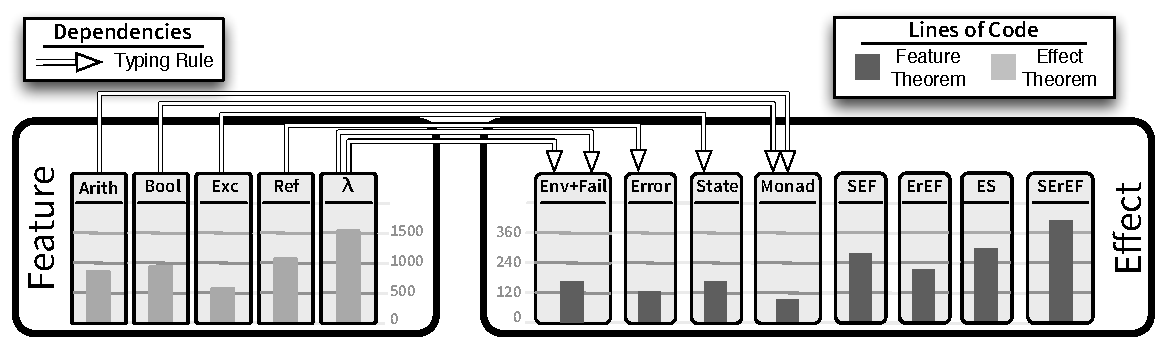
\includegraphics[scale = .85]{src/ModularEffects/CaseStudyFigure.pdf}
   }
  \end{center}
  \caption{Dependency and size information for the features and effects used in the case study.}
  \label{fig:codesize}
\end{figure*}

\section{Case Study}
\label{sec:CaseStudy}

As a demonstration of the \Name~framework, we have built a set of five
reusable language features and combined them to build a family of
languages which includes a mini-ML~\cite{clement86mini-ML} variant
with references and errors. The study includes pure boolean and
arithmetic features as well as effectful features for references,
errors and lambda abstractions.

The study builds twenty eight different combinations of the features which are
all possible combinations with at least one feature providing
values.\footnote{Also available at \url{http://www.cs.utexas.edu/~bendy/3MT}}
Figure~\ref{fig:MiniMLSyntax} presents the syntax of the expressions,
values, and types provided; each line is annotated with the feature
that provides that set of definitions.

Four kinds of feature interactions appear in the case study.

\begin{itemize}

\item The PHOAS representation of binders requires an auxiliary
equivalence relation, the details of which are covered in the MTC
paper~\cite{mtc}. The soundness proofs of language theorems for
languages which include binders proceed by induction over this
equivalence relation instead of expressions. The reusable feature
theorems of other features need to be lifted to this equivalence
relation.

\item The effect theorems that feature an environment
typing $\Sigma$, such as those for state or environment, need a weakening sublemma
which
states
that each well-formed value under
$\Sigma$ is also well-formed under a conservative extension:
\[\Sigma \vdash v ~:~ t  \\ \rightarrow \\
  \Sigma' \supseteq \Sigma \\ \rightarrow \\
  \Sigma' \vdash v ~:~ t \]
\item Inversion lemmas for the well-formed value relation as in the
proof of \ref{thm:FSound} for the boolean feature in
Section \ref{sec:Thm+Reuse} are proven by induction over the
relation.

%% \item The sublemmas of reusable feature theorems for properties such as
%% \textsc{WFM-If-Vc} are
%% proven by induction over the extensible typing relation. When effectful
%% features introduce new judgements to the relation, these new
%% judgements must have proof algebra instances for the sublemmas.

\end{itemize}


The proofs of the first and second kind of feature interactions are
straightforward; the inversion lemmas of the third kind can be
dispatched by tactics hooked into the type class inference algorithm.
%% The last kind of interactions require more work and comprise the
%% biggest part of the code dealing with feature interactions.
%%
%% The presented typing rules for effects satisfy the \textsc{WFM-Bind}
%% property; as previously discussed, it can be used cut down on feature
%% interactions. The lambda feature uses \textsc{WFM-Bind} in its proof
%% of \ref{thm:FSound} instead of targeted sublemmas. The following table
%% shows the number of sublemmas used by the reusable feature theorems,
%% highlighting that the \textsc{WFM-Bind} property provides significantly
%% more convenience despite its stronger assumptions.


The framework itself consists of about 4,400 LoC of which about 2,000
LoC comprise the implementation of the monad transformers and their
algebraic laws. The size in LoC of the implementation of semantic
evaluation and typing functions and the reusable feature theorem for
each language feature is given in the left box in Figure
\ref{fig:codesize}. The right box lists the sizes of the effect
theorems. Each language needs on average 110 LoC to assemble its
semantic functions and soundness proofs from those of its features and
the effect theorem for its set of effects.


\begin{figure}[t]
  \begin{center}
    \begin{minipage}{\columnwidth}
      \begin{center}
        \fbox{
        \hspace{-.3cm}
          \begin{tabular}{r@{~}c@{~}lr}
            {\tt e} & ::= & {\tt $\mathbb{N}$ $|$ e + e} & \textit{Arith}\\
            & $|$ &  {\tt $\mathbb{B}$ $|$ {\bf if} e {\bf then} e {\bf else} e} & \textit{Bool} \\
           %% & $|$ & {\tt {\bf case} e {\bf of \{ z} $\Rightarrow$ e $\mathbf{;}$ {\bf S} n $\Rightarrow$ e\}} & \textit{NatCase}\\
            & $|$ & {\tt {\bf lam} x : T.e $|$ e e $|$ x} & \textit{Lambda}\\
            & $|$ & {\tt {\bf ref} e $|$ !e $|$ e:=e} & \textit{References}\\
            & $|$ & {\tt {\bf try} e {\bf with} e} $|$ {\bf error} & \textit{Errors}\\
           %%  & $|$ & {\tt {\bf fix} x : T.e} & \textit{Recursion}\\
          \end{tabular}
        }
      \end{center}
    \end{minipage}
    \begin{minipage}{\columnwidth}
      \hspace{-.3cm}
    \begin{tabular}{cc}
      \begin{minipage}{.48\columnwidth}
        \fbox{
        \hspace{-.3cm}
          \begin{tabular}{r@{~}c@{~}lr}
            {\tt V} & ::= & {\tt $\mathbb{N}$} & \textit{Arith}\\
            & $|$ &  {\tt $\mathbb{B}$} & \textit{Bool} \\
            & $|$ & {\tt {\bf clos} e $\mathtt{\overline{V}}$} & \textit{Lambda}\\
            & $|$ & {\tt {\bf loc} $\mathbb{N}$} & \textit{References}\\
          \end{tabular}
        }
      \end{minipage} &
      \begin{minipage}{.38\columnwidth}
        \hspace{-.3cm}
        \fbox{
        \hspace{-.3cm}
          \begin{tabular}{r@{~}c@{~}lr}
            {\tt T} & ::= & {\tt \bf Nat} & \textit{Arith}\\
            & $|$ &  {\tt \bf Bool} & \textit{Bool} \\
            & $|$ & {\tt T $\rightarrow$ T} & \textit{Lambda}\\
            & $|$ & {\tt {\bf Ref} T} & \textit{References}\\
          \end{tabular}
        }
      \end{minipage}
    \end{tabular}
    \end{minipage}
  \end{center}
  \caption{mini-ML expressions, values, and types}
  \label{fig:MiniMLSyntax}
\end{figure}


%% \begin{center}
%%   \fbox{
%%   \hspace{-.3cm}
%%     \begin{tabular}{ c c c c c }
%%       \textit{Arith} & \textit{Bool} & \textit{Errors} & \textit{References} & \textit{Lambda} \\
%%       2 & 3 & 0 & 4 & 0 \\
%%     \end{tabular}
%%   }
%% \end{center}
%% Each sublemma of the above table requires on average 50 LoC per effect.

%% ODER: format ==         = "\mathrel{==}"
%% ODER: format /=         = "\neq "
%
%
\makeatletter
\@ifundefined{lhs2tex.lhs2tex.sty.read}%
  {\@namedef{lhs2tex.lhs2tex.sty.read}{}%
   \newcommand\SkipToFmtEnd{}%
   \newcommand\EndFmtInput{}%
   \long\def\SkipToFmtEnd#1\EndFmtInput{}%
  }\SkipToFmtEnd

\newcommand\ReadOnlyOnce[1]{\@ifundefined{#1}{\@namedef{#1}{}}\SkipToFmtEnd}
\usepackage{amstext}
\usepackage{amssymb}
\usepackage{stmaryrd}
\DeclareFontFamily{OT1}{cmtex}{}
\DeclareFontShape{OT1}{cmtex}{m}{n}
  {<5><6><7><8>cmtex8
   <9>cmtex9
   <10><10.95><12><14.4><17.28><20.74><24.88>cmtex10}{}
\DeclareFontShape{OT1}{cmtex}{m}{it}
  {<-> ssub * cmtt/m/it}{}
\newcommand{\texfamily}{\fontfamily{cmtex}\selectfont}
\DeclareFontShape{OT1}{cmtt}{bx}{n}
  {<5><6><7><8>cmtt8
   <9>cmbtt9
   <10><10.95><12><14.4><17.28><20.74><24.88>cmbtt10}{}
\DeclareFontShape{OT1}{cmtex}{bx}{n}
  {<-> ssub * cmtt/bx/n}{}
\newcommand{\tex}[1]{\text{\texfamily#1}}	% NEU

\newcommand{\Sp}{\hskip.33334em\relax}


\newcommand{\Conid}[1]{\mathit{#1}}
\newcommand{\Varid}[1]{\mathit{#1}}
\newcommand{\anonymous}{\kern0.06em \vbox{\hrule\@width.5em}}
\newcommand{\plus}{\mathbin{+\!\!\!+}}
\newcommand{\bind}{\mathbin{>\!\!\!>\mkern-6.7mu=}}
\newcommand{\rbind}{\mathbin{=\mkern-6.7mu<\!\!\!<}}% suggested by Neil Mitchell
\newcommand{\sequ}{\mathbin{>\!\!\!>}}
\renewcommand{\leq}{\leqslant}
\renewcommand{\geq}{\geqslant}
\usepackage{polytable}

%mathindent has to be defined
\@ifundefined{mathindent}%
  {\newdimen\mathindent\mathindent\leftmargini}%
  {}%

\def\resethooks{%
  \global\let\SaveRestoreHook\empty
  \global\let\ColumnHook\empty}
\newcommand*{\savecolumns}[1][default]%
  {\g@addto@macro\SaveRestoreHook{\savecolumns[#1]}}
\newcommand*{\restorecolumns}[1][default]%
  {\g@addto@macro\SaveRestoreHook{\restorecolumns[#1]}}
\newcommand*{\aligncolumn}[2]%
  {\g@addto@macro\ColumnHook{\column{#1}{#2}}}

\resethooks

\newcommand{\onelinecommentchars}{\quad-{}- }
\newcommand{\commentbeginchars}{\enskip\{-}
\newcommand{\commentendchars}{-\}\enskip}

\newcommand{\visiblecomments}{%
  \let\onelinecomment=\onelinecommentchars
  \let\commentbegin=\commentbeginchars
  \let\commentend=\commentendchars}

\newcommand{\invisiblecomments}{%
  \let\onelinecomment=\empty
  \let\commentbegin=\empty
  \let\commentend=\empty}

\visiblecomments

\newlength{\blanklineskip}
\setlength{\blanklineskip}{0.66084ex}

\newcommand{\hsindent}[1]{\quad}% default is fixed indentation
\let\hspre\empty
\let\hspost\empty
\newcommand{\NB}{\textbf{NB}}
\newcommand{\Todo}[1]{$\langle$\textbf{To do:}~#1$\rangle$}

\EndFmtInput
\makeatother
%
%
%
%
%
%
% This package provides two environments suitable to take the place
% of hscode, called "plainhscode" and "arrayhscode". 
%
% The plain environment surrounds each code block by vertical space,
% and it uses \abovedisplayskip and \belowdisplayskip to get spacing
% similar to formulas. Note that if these dimensions are changed,
% the spacing around displayed math formulas changes as well.
% All code is indented using \leftskip.
%
% Changed 19.08.2004 to reflect changes in colorcode. Should work with
% CodeGroup.sty.
%
\ReadOnlyOnce{polycode.fmt}%
\makeatletter

\newcommand{\hsnewpar}[1]%
  {{\parskip=0pt\parindent=0pt\par\vskip #1\noindent}}

% can be used, for instance, to redefine the code size, by setting the
% command to \small or something alike
\newcommand{\hscodestyle}{}

% The command \sethscode can be used to switch the code formatting
% behaviour by mapping the hscode environment in the subst directive
% to a new LaTeX environment.

\newcommand{\sethscode}[1]%
  {\expandafter\let\expandafter\hscode\csname #1\endcsname
   \expandafter\let\expandafter\endhscode\csname end#1\endcsname}

% "compatibility" mode restores the non-polycode.fmt layout.

\newenvironment{compathscode}%
  {\par\noindent
   \advance\leftskip\mathindent
   \hscodestyle
   \let\\=\@normalcr
   \let\hspre\(\let\hspost\)%
   \pboxed}%
  {\endpboxed\)%
   \par\noindent
   \ignorespacesafterend}

\newcommand{\compaths}{\sethscode{compathscode}}

% "plain" mode is the proposed default.
% It should now work with \centering.
% This required some changes. The old version
% is still available for reference as oldplainhscode.

\newenvironment{plainhscode}%
  {\hsnewpar\abovedisplayskip
   \advance\leftskip\mathindent
   \hscodestyle
   \let\hspre\(\let\hspost\)%
   \pboxed}%
  {\endpboxed%
   \hsnewpar\belowdisplayskip
   \ignorespacesafterend}

\newenvironment{oldplainhscode}%
  {\hsnewpar\abovedisplayskip
   \advance\leftskip\mathindent
   \hscodestyle
   \let\\=\@normalcr
   \(\pboxed}%
  {\endpboxed\)%
   \hsnewpar\belowdisplayskip
   \ignorespacesafterend}

% Here, we make plainhscode the default environment.

\newcommand{\plainhs}{\sethscode{plainhscode}}
\newcommand{\oldplainhs}{\sethscode{oldplainhscode}}
\plainhs

% The arrayhscode is like plain, but makes use of polytable's
% parray environment which disallows page breaks in code blocks.

\newenvironment{arrayhscode}%
  {\hsnewpar\abovedisplayskip
   \advance\leftskip\mathindent
   \hscodestyle
   \let\\=\@normalcr
   \(\parray}%
  {\endparray\)%
   \hsnewpar\belowdisplayskip
   \ignorespacesafterend}

\newcommand{\arrayhs}{\sethscode{arrayhscode}}

% The mathhscode environment also makes use of polytable's parray 
% environment. It is supposed to be used only inside math mode 
% (I used it to typeset the type rules in my thesis).

\newenvironment{mathhscode}%
  {\parray}{\endparray}

\newcommand{\mathhs}{\sethscode{mathhscode}}

% texths is similar to mathhs, but works in text mode.

\newenvironment{texthscode}%
  {\(\parray}{\endparray\)}

\newcommand{\texths}{\sethscode{texthscode}}

% The framed environment places code in a framed box.

\def\codeframewidth{\arrayrulewidth}
\RequirePackage{calc}

\newenvironment{framedhscode}%
  {\parskip=\abovedisplayskip\par\noindent
   \hscodestyle
   \arrayrulewidth=\codeframewidth
   \tabular{@{}|p{\linewidth-2\arraycolsep-2\arrayrulewidth-2pt}|@{}}%
   \hline\framedhslinecorrect\\{-1.5ex}%
   \let\endoflinesave=\\
   \let\\=\@normalcr
   \(\pboxed}%
  {\endpboxed\)%
   \framedhslinecorrect\endoflinesave{.5ex}\hline
   \endtabular
   \parskip=\belowdisplayskip\par\noindent
   \ignorespacesafterend}

\newcommand{\framedhslinecorrect}[2]%
  {#1[#2]}

\newcommand{\framedhs}{\sethscode{framedhscode}}

% The inlinehscode environment is an experimental environment
% that can be used to typeset displayed code inline.

\newenvironment{inlinehscode}%
  {\(\def\column##1##2{}%
   \let\>\undefined\let\<\undefined\let\\\undefined
   \newcommand\>[1][]{}\newcommand\<[1][]{}\newcommand\\[1][]{}%
   \def\fromto##1##2##3{##3}%
   \def\nextline{}}{\) }%

\newcommand{\inlinehs}{\sethscode{inlinehscode}}

% The joincode environment is a separate environment that
% can be used to surround and thereby connect multiple code
% blocks.

\newenvironment{joincode}%
  {\let\orighscode=\hscode
   \let\origendhscode=\endhscode
   \def\endhscode{\def\hscode{\endgroup\def\@currenvir{hscode}\\}\begingroup}
   %\let\SaveRestoreHook=\empty
   %\let\ColumnHook=\empty
   %\let\resethooks=\empty
   \orighscode\def\hscode{\endgroup\def\@currenvir{hscode}}}%
  {\origendhscode
   \global\let\hscode=\orighscode
   \global\let\endhscode=\origendhscode}%

\makeatother
\EndFmtInput
%
%
%
% First, let's redefine the forall, and the dot.
%
%
% This is made in such a way that after a forall, the next
% dot will be printed as a period, otherwise the formatting
% of `comp_` is used. By redefining `comp_`, as suitable
% composition operator can be chosen. Similarly, period_
% is used for the period.
%
\ReadOnlyOnce{forall.fmt}%
\makeatletter

% The HaskellResetHook is a list to which things can
% be added that reset the Haskell state to the beginning.
% This is to recover from states where the hacked intelligence
% is not sufficient.

\let\HaskellResetHook\empty
\newcommand*{\AtHaskellReset}[1]{%
  \g@addto@macro\HaskellResetHook{#1}}
\newcommand*{\HaskellReset}{\HaskellResetHook}

\global\let\hsforallread\empty

\newcommand\hsforall{\global\let\hsdot=\hsperiodonce}
\newcommand*\hsperiodonce[2]{#2\global\let\hsdot=\hscompose}
\newcommand*\hscompose[2]{#1}

\AtHaskellReset{\global\let\hsdot=\hscompose}

% In the beginning, we should reset Haskell once.
\HaskellReset

\makeatother
\EndFmtInput

% format runC         = "run\mathbb{C}_{\scalebox{0.6}{T}}"
% format C            = "\mathbb{C}_{\scalebox{0.6}{T}}"
%%format R            = "\mathbb{R}_{\scalebox{0.6}{T}}"


\section{Related and Future Work}

\paragraph{DGP in proof-assistants}

Datatype-generic programming started out as a form of language
extension such as PolyP \cite{jansson:polyp} or Generic Haskell
\cite{loh:dsgh}. Yet Haskell has turned out to be powerful enough to
implement datatype-generic programming in the language itself and over
the time a vast number of DGP libraries for Haskell have been proposed
\cite{cheney:ligd,syb,emgm,multirec,instantgenerics,uniplate,genericderiving}. Compared
with a language extension, a library is much easier to develop and
maintain.

Using the flexibility of dependent-types there are multiple proposals
for performing datatype-generic programming in proof assistants
\cite{dgpcoq,altenkirch:gpwdtp,benke:universes,loh:gpif,indexedcontainers}. This
setting not only allows the implementation of generic functions, but
also of generic proofs. The approaches vary in terms of how strictly
they follow the positivity or termination restrictions imposed by the
proof assistant. Some circumvent the type-checker at various points to
simplify the development or presentation while others put more effort
in convincing the type-checker and termination checker of the validity
\cite{ertt}. However, in all of the proposals there does not seem to
be any fundamental problem caused by the restrictions.


\paragraph{DGP for modular proofs}

Modularly composing semantics and proofs about the semantics has also
been addressed by \cite{schwaab:mtp} in the context of programming
language meta-theory. They perform their development in Agda and
similar to our approach they also use a universe approach based on
polynomial functors to represent modular datatypes. They split
relations for small-step operational semantics and well-typing on a
feature basis. However, the final fixed points are constructed manually
instead of having a generic representation of inductive families.

Using Coq's type classes both MTC and our approach also allow for more
automation in the final composition of datatypes, functions and
proofs. Agda features instance arguments that can be used to replace
type classes in various cases. However, the current implementation
does not perform recursive resolution and as a result Agda does not
support automation of the composition to the extent that is needed for
DTC-like approaches.


\paragraph{Combining different DGP approaches}

We have shown an embedding of the universe of polynomial functors into
the universe of containers. Similar inclusions between universes have
been done in the literature \cite{morris:cspf}. Magalh\~aes and L\"oh
\cite{jpm:fcadgp} have ported several popular DGP approaches from
Haskell to Agda and performed a formal comparison by proving inclusion
relations between the approaches.

DGP approaches differ in terms of the class of datatypes they capture and the
set of generic functions that can be implemented for them. Generic functions
can be transported from a universe into a sub-universe. However, we are not
aware of any DGP library with a systematic treatment of universes where each generic
function is defined on the most general universe that supports that function.


\paragraph{DGP for abstract syntax}

We have shown how to obtain more reuse by complementing modular
definitions with a generic equality function and generic proofs of its
properties. Of course more generic functionality like traversals,
pretty-printing, parsing etc. can be covered by means of
datatype-generic programming.

One very interesting idea is to use datatype-generic programming to
handle variable binding \cite{cheney:synp,unbound}. Variable
binding is an ubiquitous aspect of programming languages. Moreover, a
lot of functionality like variable substitutions and free variable
calculations is defined for many languages. Licata and Harper
\cite{licata:ubc} and Keuchel and Jeuring \cite{sk:gcasr} define
universes for datatypes with binding in Agda. Lee et al.~\cite{gmeta}
develop a framework for first-order representations of variable
binding in Coq that is based on the universe of regular tree types
\cite{ertt} and that provides many of the so-called
\emph{infrastructure lemmas} required when mechanizing programming
language meta-theory.

An interesting direction for future work is to extend these approaches
to capture variable binding in the indices of relations on abstract
syntax and use this as the underlying representation of extensible
datatypes and extensible logical relations and thereby complementing
modular functions with generic proofs about variable binding.


\paragraph{Automatic derivation of instances}

Most, if not all, generic programming libraries in Haskell use Template
Haskell to derive the generic representation of user-defined types and
to derive the conversion functions between them.

The GMeta \cite{gmeta} framework includes a standalone tool that also
performs this derivation for Coq. Similarly we also like to be able
to derive instances for the \ensuremath{\Conid{Container}} and \ensuremath{\Conid{Polynomial}} classes
automatically.


Formally mechanizing proofs can be very tedious and the amount of work
required for larger developments is excruciating. Meta-Theory \`a la Carte
is a framework for modular reusable components for use in
mechanizations. It builds on the Datatypes \`a la Carte approach to solve
an extended version of the expression problem. MTC allows modular
definitions of datatypes, semantic functions and logical relations and
furthermore modular inductive proofs.

MTC uses extensible Church-encodings to overcome conservative restrictions
imposed by the Coq proof-assistant. This approach has shortcomings
in terms of confidence in the definitions and in terms of usability. This
paper addresses these shortcomings by using datatype-generic
programming techniques to replace Church-encodings as the underlying representation
of type-level fixed points. Our approach avoids impredicativity, adequately
encodes fixed points and leads to stronger induction principles by
exploiting DGP approaches that capture only strictly-positive functors.

Working with generic structure representation has the added benefit that
we can implement generic functions like equality and generic proofs once and for all.


}
\part{Genericity}\label{part:gen}
{
\newcommand{\ov}[1]{\overline{#1}}
\newcommand{\cpar}[1]{{\texttt{(}{#1}\texttt{)}}}
\newcommand{\cbrc}[1]{{\texttt{\{}{#1}\texttt{\}}}}
\newcommand{\cbrk}[1]{{\texttt{[}{#1}\texttt{]}}}
\newcommand{\ccol}{\texttt{:}}
\newcommand{\cass}{\texttt{:=}}
\newcommand{\cto}{~\texttt{->}~}

\newcommand{\fieldref}[2]{\cpar{{#1}\,\texttt{@}\,{#2}}}
\newcommand{\fieldbind}[2]{\cpar{{#1}\,\ccol\,{#2}}}
\newcommand{\fieldsub}[2]{\cpar{{#1}\,\ccol\,{#2}}}
\newcommand{\evalbs}[2]{{\llbracket\:{#1}\:\rrbracket_{#2}}}
\newcommand{\evalbig}[3]{[{#1}] {#2} \Downarrow {#3}}
\newcommand{\evalbigf}[3]{{#1}({#2}) \Downarrow {#3}}
\newcommand{\evalsym}[3]{{\llbracket\: {#1} \mid {#2} \:\rrbracket_{#3}}}
\newcommand{\evalrbs}[4]{{\llbracket\: {#1} \:\rrbracket_{{#3},{#4}}}}
\newcommand{\symflatten}[3]{{{#1} \vdash_E {#2} \Downarrow {#3}}}

\newcommand{\typing}[3]{{#1} \vdash_\text{tm} {#2} : {#3}}

\newcommand{\fprod}{\ensuremath{F_\times}\xspace}
\newcommand{\POPLmark}{\textsc{POPLmark}\xspace}
\newcommand{\LNGen}{\textsc{LNGen}\xspace}
\newcommand{\DbGen}{\textsc{DbGen}\xspace}
\newcommand{\Ott}{\textsc{Ott}\xspace}
\newcommand{\Romeo}{\textsc{Romeo}\xspace}
\newcommand{\AutoSubst}{\textsc{AutoSubst}\xspace}
\newcommand{\GMeta}{\textsc{GMeta}\xspace}
\newcommand{\SystemF}{System~F\xspace}
\newcommand{\SystemFsub}{\ensuremath{\text{System~F}_{<:}}\xspace}
\newcommand{\LF}{\textlambda LF\xspace}
\newcommand{\CoC}{\textsc{CoC}\xspace}
\newcommand{\stlc}{\ensuremath{\lambda}\xspace}
\newcommand{\stlcprod}{\ensuremath{\lambda_{\times}}\xspace}
\newcommand{\F}{\ensuremath{F}\xspace}
\newcommand{\fsub}{\ensuremath{F_{<:}}}
\newcommand{\fsubprod}{\ensuremath{F_{<:,\times}}}
\newcommand{\Unbound}{\textsc{Unbound}\xspace}
\newcommand{\lomega}{\ensuremath{\lambda_{\omega}}\xspace}
\newcommand{\fomega}{\ensuremath{F_{\omega}}\xspace}
\newcommand{\fseqlet}{\ensuremath{F_\text{seq}}}
\newcommand{\fsubrcd}{\ensuremath{F_{<:,\text{rcd}}}}
\newcommand{\fexists}{\ensuremath{F_{\exists}}\xspace}
\newcommand{\fexistsprod}{\ensuremath{F_{\exists,\times}}\xspace}

\newcommand{\spec}{\mathit{spec}}
\newcommand{\decl}{\mathit{decl}}
\newcommand{\namedecl}{\mathit{namedecl}}

\newcommand{\knotkeyword}[1]{{\texttt{#1}}}
\newcommand{\namespace}{\knotkeyword{namespace}}
\newcommand{\sort}{\knotkeyword{sort}}
\newcommand{\function}{\knotkeyword{fun}}
\newcommand{\env}{\knotkeyword{env}}
\newcommand{\relation}{\knotkeyword{relation}}
\newcommand{\subst}{\knotkeyword{subst}}
\newcommand{\In}{\knotkeyword{In}}

\newcommand{\sortdecl}{\mathit{sortdecl}}
\newcommand{\condecl}{\mathit{condecl}}
\newcommand{\bsi}{\mathit{bsi}}
\newcommand{\bindspec}{\mathit{bs}}
\newcommand{\fundecl}{\mathit{fundecl}}
\newcommand{\funclause}{\mathit{funclause}}

\newcommand{\envdecl}{\mathit{envdecl}}
\newcommand{\envclause}{\mathit{envclause}}
\newcommand{\reldecl}{\mathit{reldecl}}
\newcommand{\ruledecl}{\mathit{ruledecl}}
\newcommand{\formula}{\mathit{fml}}
\newcommand{\lookup}{\mathit{lookup}}
\newcommand{\jmv}{\mathit{j}}
\newcommand{\judgement}{\mathit{jmt}}
\newcommand{\rulebindspec}{\mathit{rbs}}
\newcommand{\rbsi}{\mathit{rbsi}}
\newcommand{\symbolicterm}{\mathit{sym}}
\newcommand{\symboliccoterm}{\mathit{cosym}}
\newcommand{\symbolicweaken}{\mathbf{weaken}}
\newcommand{\symboliccoweaken}{\mathbf{coweaken}}
\newcommand{\symbolicsubst}{\mathbf{subst}}
\newcommand{\symbolicenv}{\theta}
\newcommand{\LENV}{\mathcal{L}}
\newcommand{\VENV}{\mathcal{V}}
\newcommand{\RENV}{\mathcal{R}}
\newcommand{\dom}{\text{dom}}
\newcommand{\domain}[1]{{\dom~{#1}}}

\newcommand{\wfbindspec}[3]{\LENV; {#1} \vdash {#2}}  %  : {#3}
\newcommand{\wfsym}[3]{\LENV; {#1} \vdash {#2} : {#3}}
\newcommand{\wfruledecl}[4]{\vdash_{#1,#2,#3} #4}
\newcommand{\wfformula}[2]{\LENV \vdash_{#1} {#2}}

\newcommand{\judg}[4]{{#1} \models_{#2} {#3} ; {#4}}
\newcommand{\judgsimpl}[3]{{#1} \models_{#2} {#3}}
\newcommand{\lookupenv}[5]{{ ({#1}:{#2}) \in_{{#3},{#4}} {#5}}}

\newcommand{\eqtreflcon}{\text{qrf}}
\newcommand{\eqttranscon}{\text{qtr}}
\newcommand{\eqtsymcon}{\text{qsm}}
\newcommand{\eqtregcon}{\text{qcn}}

\newcommand{\Eqh}[4]{\models_{#1} {#2} : {#3} \equiv {#4}}
\newcommand{\Equ}[6]{{#1} \equiv {#2} \models_{#3} {#4} : {#5} \equiv {#6}}

\newcommand{\eqt}{\text{eqt}}
\newcommand{\eqtrefl}[3]{\eqtreflcon~{#1}~{#2}~{#3}}
\newcommand{\eqttrans}[2]{\eqttranscon~{#1}~{#2}}
\newcommand{\eqtsym}[1]{\eqtsymcon~{#1}}
\newcommand{\eqtreg}[2]{\eqtregcon~{#1}~{#2}}
\newcommand{\sh}[3]{\text{sh}_{#1}~{#2}~{#3}}
\newcommand{\su}[4]{\text{su}_{#1}~{#2}~{#3}~{#4}}
\newcommand{\shstar}{{\text{sh}^{*}}}
\newcommand{\wk}[2]{\shstar~{#1}~{#2}}
\newcommand{\eqtshiftweaken}[2]{\text{qhw}~{#1}~{#2}}
\newcommand{\eqtshiftsubst}[2]{\text{qhu}~{#1}~{#2}}
\newcommand{\eqtsubstweaken}[1]{\text{quw}~{#1}}
\newcommand{\eqtsubstsubst}[1]{\text{quu}~{#1}}
\newcommand{\eqtcongweaken}[2]{\text{qcw}~{#1}~{#2}}
%% \newcommand{\eqterm}[8]{\LENV;{#1};{#2};{#3} \models {#4} : ({#5} \vdash {#6} = {#7} : {#8})}
\newcommand{\eqterm}[8]{{#4} \models_{\LENV,{#1},{#2},{#3}} ({#5} \vdash {#6} = {#7} : {#8})}
\newcommand{\knotbox}[1]{{\hspace{-1em}\framebox{\mbox{\ensuremath{#1}}}}}

\newcommand{\wsterm}[7]{({#3}) \models_{#5} ({#4} \vdash_{#7} {#6})}
\newcommand{\wnindex}[7]{({#3}) \models_{#5} ({#4} \vdash_{#7} {#6})}

\newcommand{\igfunclause}[2]{ #1 \equiv #2 \\}
\newcommand{\ignt}[1]{\mathit{#1}}
\newcommand{\igmv}[1]{\mathit{#1}}
\newcommand{\igkw}[1]{\mathbf{#1}}
\newcommand{\igsym}[1]{#1}
\newcommand{\igcom}[1]{\text{#1}}
\newcommand{\igdrulename}[1]{\textsc{#1}}
\newcommand{\igcomplu}[5]{\overline{#1}^{\,#2\in #3 #4 #5}}
\newcommand{\igcompu}[3]{\overline{#1}^{\,#2<#3}}
\newcommand{\igcomp}[2]{\overline{#1}^{\,#2}}

%%% Local Variables:
%%% mode: latex
%%% TeX-master: "Main"
%%% End:


\chapter{Background}
{ % STLCBOOL SCOPE

\newcommand{\stlcbool}{\ensuremath{\lambda_{\mathbb{B}}}\xspace}
\newcommand{\bool}{\text{bool}}
\newcommand{\true}{\textbf{true}\xspace}
\newcommand{\false}{\textbf{false}\xspace}
\newcommand{\ite}[3]{\textbf{if}~{#1}~\textbf{then}~{#2}~\textbf{else}~{#3}}
\newcommand{\typing}[3]{{#1} \vdash {#2} : {#3}}
\renewcommand{\eval}[2]{{#1} \longrightarrow {#2}}
\newcommand{\evals}[2]{{#1} \longrightarrow^* {#2}}

\chapter{Introduction}

The concept of programming can be defined as communicating how to perform tasks
to a computer. An increasing number of fields such as biology, engineering,
physics, psychology and sociology rely on programming. Programming is not
limited to sciences. The ubiquity of computers and the pervasive use of software
in our society indirectly depend on programming and programmers.  However,
software is notoriously unreliable. Given the extent of our dependence on
software this is all the more detrimental and costly.

In order to improve upon this situation we need to meliorate the process of
programming itself.
\begin{itemize}
\item 'Programming languages' are the tools/methods for programming
\item The minimum requirement is that a program does what it's intended to do.
\end{itemize}

For a programmer it is essential that she can validate that a program implements
exactly the intended task which is usually achieved by reasoning with the
\emph{expected behaviour} of a program.

But how is the behaviour of programming constructs defined, or more generally,
how are programming languages defined? The majority of programming languages
start with a reference implementation that effectively defines the language.
% Examples of languages that are (still) defined this way include Perl -
% Perl~5~\cite{perllanguage} and Python~\cite{pythonlanguage}.

After widespread use, a language may go through a standardization process:
multiple stakeholders develop a common language specification.
% , e.g. PHP was standardized in 2014~\cite{phpspec}.
Another approach is develop specifications together with a reference
implementation. These two approaches are not mutually exclusive: languages with
an existing specification are extended in tandem with implementations.

Such a language specification allows a programmer to resolve ambiguities when
reasoning about her programs independent of a particular implementation. It also
enables us to switch between implementations.

Programming language theory is a branch of computer science that deals with
language specifications, design, implementation, and in particular also
meta-theoretical analysis of programming languages, their semantics and related
systems like type-systems. When developing new languages or language features we
want to make sure that the design is coherent and fulfills the expectations of
users.

The programmer is often given useful safety guarantees for this programs. For
instance, many modern programming language provide garbage collection
facilities. Yet we want our programs to be memory safe, i.e. they do not access
memory that has been freed or that has not yet been initialized. Another safety
property is type-safety, i.e. the absence of dynamic type errors during
execution. These guarantees are usually provided for all programs written in a
language or a specific subset of programs, e.g. all type-checked programs. In a
meta-theoretical analysis we want to make sure that these are indeed valid
guarantees.

The meta-theory of programming language semantics and type-systems is highly
complex due to the management of many details and edge cases. As such, it is
prone to subtle errors that can invalidate large amounts of work.

For example, the Java programming language was long believed to be type-safe
\footnote{Except for some deliberate defects like the co-variance of arrays.}
but the addition of Generics made Java's type system in fact unsound
\cite{amin2016java}. Another problem concerns the type-checking of Java
programs. Generics made type-checking an undecidable property of
programs~\cite{grigore2017}. Decidability of type-checking does not have an
impact on properties that we get for type-checked programs, but for example it
opens up attack vectors on (web) services that deal with Java code because the
type-checker may run forever.

To increase the confidence in the correctness of formal meta-theory, techniques
for formalization in proof-assistants, also known as mechanization, have
received much attention. These systems allow us to state mathematical statements
and proofs for them and let the machine check that these are in fact valid
proofs. However, the high development cost of mechanizations continues to
prevent their widespread use. This leads us to the research question that this
thesis tries to answer:

\begin{center}
  \begin{minipage}{0.8\columnwidth}
    How can we reduce the costs of mechanizing formal meta-theory of programming
    languages?
  \end{minipage}
\end{center}

\begin{itemize}
\item Current methodology.
\item Why is the current methodology costly?
\item Give an idea of the relative effort.
\item What is the approach answer of this thesis?

  Increase reusability of code. Two strands: Modularity / Genericity.
\end{itemize}




The remainder of this chapter will give a more detailed introduction to the
relevant disciplines of specification, analysis and mechanization of programming
languages similar to what can be found in introductory textbooks such as
\cite{tapl}.

%% %-------------------------------------------------------------------------------
%% \section{Mechanization}
%% Mechanizing formal meta-theory in proof-assistants is crucial, both for the
%% increased confidence in complex designs and as a basis for technologies such as
%% proof-carrying code.  Formal reasoning in proof-assistants, also known as
%% mechanization, has high development costs.
%%

%% \begin{itemize}
%% \item
%%   Derive properties for all programs written in a language, like memory-safety,
%%   type-safety, resources-safety, termination, absence of deadlocks, race
%%   conditions and starvation.
%%
%% \item
%%   Prove correctness (preservation of semantics) of program analyses or compiler
%%   transformations.
%%
%%   by looking formally on the semantics, type systems and implementations like
%%   compilers or interpreters.
%% \end{itemize}

%-------------------------------------------------------------------------------
\section{Specifications}\label{sec:intro:specification}

%% Standardization and functional or program specifications are an essential
%% methodology in systems engineering and software development. It serves as the
%% baseline for correctness of implementations. Furthermore, multiple
%% implementations that are correct with respect to a common specification are
%% inter-operable or compatible to a certain extent. The precise meaning depends
%% on the context and the requirements.
%%
%% For programming languages for example, we want to guarantee that the same
%% program is executable by different implementations and performs the same
%% tasks.  This does for example also ensures that program analyses and program
%% transformations, e.g. for optimization, can be developed independent of a
%% particular implementation and adopted by multiple implementations.
%%
%% In this thesis, we are interested in programming languages themselves and not
%% so much interested in their implementations. Hence, a specification of a
%% application binary interface, for example, to achieve binary compatibility of
%% modules compiled by different compilers is beyond the scope of this thesis.

Specifications differ in the detail and precision they describe systems.
Industrial specifications of major programming languages are usually written in
natural language and are detailed to cover every aspect of the languages. The
use of natural language leaves opportunities for ambiguity, but disregarding
this problem, elaborate industrial specifications provide a good reference point
for language users and implementors. However, for meta-theoretical analyses more
rigorous specifications are necessary.

We will use \emph{formal specifications} and a mathematical language to
describe programming languages. This gives use the necessary precision and
avoids the ambiguities of natural languages. This section explains necessary
fundamental concepts for the formal specification of programming languages by
example of a small language \stlcbool: a simply-typed lambda calculus with
booleans. We specify the \emph{abstract syntax}, \emph{static type system} and
\emph{evaluation} of \stlcbool using inductive definitions. Along the way, we
define the terminology and notational conventions and make their meaning
precise.

%-------------------------------------------------------------------------------
\subsection{Syntax}\label{ssec:intro:syntax}

\begin{figure}[t]
  \centering
  \fbox{
    \begin{minipage}{\columnwidth}
    \begin{tabular}{lcll}
      $x,y$           & ::=    &                            & term variable    \\
      $\tau,\sigma$   & ::=    &                            & type             \\
                      & $\mid$ & $\tau \to \tau$            & function type    \\
                      & $\mid$ & $\bool$                    & boolean type     \\
      $e$             & ::=    &                            & term             \\
                      & $\mid$ & $\true$                    & true constant    \\
                      & $\mid$ & $\false$                   & false constant   \\
                      & $\mid$ & $\ite{e}{e}{e}$            & conditional      \\
                      & $\mid$ & $x$                        & term variable    \\
                      & $\mid$ & $\lambda x:\tau.e$         & term abstraction \\
                      & $\mid$ & $e~e$                      & application      \\
      $v$             & ::=    &                            & term             \\
                      & $\mid$ & $\true$                    & true constant    \\
                      & $\mid$ & $\false$                   & false constant   \\
                      & $\mid$ & $\lambda x:\tau.e$         & term abstraction \\
      $\Gamma$        & ::=    &                            & type context     \\
                      & $\mid$ & $\epsilon$                 & empty context    \\
                      & $\mid$ & $\Gamma, x:\tau$           & term binding     \\
    \end{tabular}
    \end{minipage}
  }
  \caption{\stlcbool syntax}
  \label{fig:intro:stlcboolsyntax}
\end{figure}

The syntax of \stlcbool is given in Figure \ref{fig:intro:stlcboolsyntax}. We
use a convention that is close to standard \textsc{EBnf} grammars. Elided in the
grammar are syntactic constructs like parentheses. We use parentheses freely to
resolve ambiguities in terms even if the grammar does not define them. Any
implementation that deals with the concrete syntax of a programming language has
of course to be more rigorous.

The grammar in Figure \ref{fig:intro:stlcboolsyntax} defines several
\emph{syntactic sorts} for \stlcbool. The \emph{meta-variable} $e$ stands for
expressions of \stlcbool of which there are 6 different kinds. An expression can
either be a boolean constant $\true$ or $\false$, a conditional form
$\ite{e_c}{e_t}{e_e}$, an \emph{object-language variable} (represented by the
meta-variable $x$), the definition of a function as a \textlambda-abstraction
$(\lambda x:\tau.e)$ or the application of an expression $e_1$ to another
expression $e_2$. Of course we only want to apply expressions $e_1$ that
represent functions: either by being a \textlambda-abstraction or evaluating to
one. Applying any \emph{value} other than a \textlambda-abstraction is a
\emph{type error}. We make this more precise below and come back to it it
Section \ref{sec:intro:typesafety} on analysis.

The grammar also includes the meta-variable $\tau$ that describes the types of
\stlcbool. Each \textlambda-abstraction contains a \emph{type annotation} $\tau$
for the argument variable $x$. The denotation is that the function represented
by the \textlambda-abstraction expects a value of type $\tau$ when it is
applied. We discuss types and typing contexts $\Gamma$ in more detail in Section
\ref{ssec:intro:typing} which deals with static typing.


%-------------------------------------------------------------------------------
\subsection{Semantics}\label{ssec:intro:semantics}

We have defined the syntax of \stlcbool expressions and can now turn towards
defining their meaning. There are multiple established ways to define semantics
of programming language. We can coarsely classify the approaches into three
different groups:

\begin{enumerate}
\item Operational Semantics

  Operational semantics defines the meaning of programs by specifying their
  execution in a state transition system. A \emph{state transition function} or
  a \emph{state transition relation} on the terms of the programming language
  defines the possible execution steps. The program is part of the state. For
  small languages the entire state might consist of only the program. After
  taking a step we are left with an updated state that includes a residual
  program.

  %% We can then define the meaning of programs to be the execution process on
  %% the abstract machine.


\item Denotational Semantics

  Denotational semantics defines the meaning of programs in terms of collection
  of \emph{mathematical semantic domains} that can include numbers, sets or
  functions. An \emph{interpretation function} maps program terms into these
  domains. This function is generally compositional in the syntax which
  is beneficial for modularity.

  Usually, the semantic domain has an established \emph{formal theory}. The
  theorems of the domain give rise to reasoning laws for programs. Furthermore,
  we can also derive properties of programming languages from properties of the
  collection of semantic domains.

\item Axiomatic Semantics

  Instead of deriving laws for programs from their execution behaviour or
  denotation we can also axiomatically assume these laws. This is known as an
  axiomatic semantics.

  This gives us immediately the means for reasoning about programs. Furthermore,
  we can derive a denotational semantics for the language by constructing a
  model that satisfies the chosen laws and derive properties for this model or
  even all models.

\end{enumerate}

These approaches have different trade-offs. Denotational and axiomatic semantics
immediately give us powerful mathematical tools to reason about programming
languages and their programs, but for larger languages the required technicality
and complexity makes it extremely difficult to even define a suitable semantics.

Operational semantics do not give us the same powerful mathematical reasoning
techniques and instead impose on us the laborious task to reason about programs
by observing their behaviour during execution. However, operational semantics
are simpler and easier to define than more abstract denotational or axiomatic
semantics. Moreover, they are much closer to actual implementations. Due to the
smaller gap, operational semantics make it easier to reason about the
correctness of implementations.

\begin{figure}[t]
  \centering
  \fbox{
    \begin{minipage}{\columnwidth}
      \framebox{\mbox{$\eval{e}{e}$}}\\
      \vspace{-5mm}
      \[ \begin{array}{c}
           \inferrule* [right=\textsc{EIfTrue},]
             {
             }
             {\eval{\ite{\true}{e_t}{e_e}}{e_t}
             } \\\\
           \inferrule* [right=\textsc{EIfFalse}]
             {
             }
             {\eval{\ite{\false}{e_t}{e_e}}{e_e}
             } \\\\
           \inferrule* [right=\textsc{EIf}]
             {\eval{e_c}{e_c'}
             }
             {\eval{\ite{e_c}{e_t}{e_e}}{\ite{e_c'}{e_t}{e_e}}
           } \\\\
           \inferrule* [right=\textsc{EAppAbs}]
             {
             }
             {\eval{(\lambda x:\tau.e_1)~e_2}{[x \mapsto e_2]e_1}
             } \\\\
           \inferrule* [right=\textsc{EApp}]
             {\eval{e_1}{e_2'}
             }
             {\eval{e_1~e_2}{e_1'~e_2}
             } \\\\
         \end{array}
       \]
    \end{minipage}
  }
  \caption{\stlcbool reduction rules}
  \label{fig:intro:stlcbooleval}
\end{figure}

For our \stlcbool language we define semantics using a \emph{small-step
  operational semantics}. This is also the approach used in Part \ref{part:gen}
of this thesis. Part \ref{part:mod} uses denotational semantics.

Figure \ref{fig:intro:stlcbooleval} gives the complete definition of the
operational semantics by means of an evaluation relation. The box in the upper
left corner \framebox{\mbox{$\eval{e_1}{e_2}$}} defines the shape and notation
that we use for the relation. In this case it is a binary relation between two
terms, which denotes that $e_1$ evaluates to $e_2$ in one step.

The remainder of the figure defines the relation using Gentzen-style inference
rules~\cite{gentzen1935}. In general, rules take the form
\[
  \inferrule* [right=\textsc{Name}]
    {J_1 \\ J_2 \\ \ldots \\ J_n
    }
    {J
    }
\]
where \textsc{Name} is an optional name for the rule that allows us to refer to
it. The meta-variable $J$ stands for judgements, which in our case are usually
mathematical statements in propositional or first-order logic. The judgements
$J_1, \ldots, J_n$ above the horizontal line are the premises of the rule, and
the judgement $J$ below the line is the conclusion. Rule without any premises
are also called \emph{axioms}. The conclusion will always involve the relation
that is being defined.

The single-step evaluation is defines using five rules. The two axioms
\textsc{EIfTrue} and \textsc{EIfFalse} show how to reduce an
\textbf{if}-expression in case the condition is either a \true or a \false
value. The case of a condition that is not yet fully evaluated is handled by
rule \textsc{EIf}. If the condition $e_c$ reduces to $e_c'$ in one step then we
can conclude the one step reduction
\[ \eval{\ite{e_c}{e_t}{e_e}}{\ite{e_c'}{e_t}{e_e}} \]

The last two rules cover the evaluation of \textlambda-terms. The rule
\textsc{EAppAbs} handles the case where the left-hand side of an application is
a \textlambda-term $(\lambda x:\tau.e_1)$. The residual program is the the body
$e_1$ of the function after substituting $e_2$ for $x$ which we write as
$[x \mapsto e_2]e_1$. The argument of the function does not have to be fully
evaluated, i.e. the rules encode a \emph{call-by-name} evaluation strategy. If
the left-hand side is not yet a \textlambda-term, we evaluate it first similarly
to \textsc{EIf}.

Note that this definition does not cover all the cases. In particular
the case of a \textlambda-term in the condition of an \textbf{if}-expression
\[ \ite{(\lambda x:\tau.e)}{e_t}{e_e} \]
\noindent and the cases of a boolean in the left-hand side of an application
\[ \true~e_1 \qquad \text{or} \qquad \false~e_2 \]
\noindent are not specified. Since no transition is defined and the execution
stopped without any \emph{meaningful result}, we also say that the evaluation
got stuck. In an implementation of the programming language, this corresponds to
an error that can happen during execution of a program. It's therefore also
called a \emph{(dynamic) type error}. Programmers want to detect potential
problems like that early in the development cycle and, if possible, at compile
time. This motivates the development of \emph{static type systems}.

%-------------------------------------------------------------------------------
\subsection{Typing}\label{ssec:intro:typing}

\begin{figure}[t]
  \centering
  \fbox{
    \begin{minipage}{\columnwidth}
      \framebox{\mbox{$\typing{\Gamma}{e}{\tau}$}}\\
      \vspace{-5mm}
      \[ \begin{array}{c}
           \inferrule* [right=\textsc{TTrue}]
             {
             }
             {\typing{\Gamma}{\true}{\bool}
             } \quad
           \inferrule* [right=\textsc{TFalse}]
             {
             }
             {\typing{\Gamma}{\false}{\bool}
             } \\\\
           \inferrule* [right=\textsc{TIf}]
             {\typing{\Gamma}{e_c}{\bool} \\
              \typing{\Gamma}{e_t}{\tau} \\
              \typing{\Gamma}{e_e}{\tau}
             }
             {\typing{\Gamma}{\ite{e_c}{e_t}{e_e}}{\tau}
             } \\\\
           \inferrule* [right=\textsc{TVar}]
             {x : \tau \in \Gamma
             }
             {\typing{\Gamma}{x}{\tau}
             } \quad
           \inferrule* [right=\textsc{TAbs}]
             {\typing{\Gamma,y:\sigma}{e}{\tau}
             }
             {\typing{\Gamma}{(\lambda y:\sigma. e)}{(\sigma\to\tau)}
             } \\\\
           \inferrule*[right=\textsc{TApp}]
             {\typing{\Gamma}{e_1}{\sigma \to \tau} \\
              \typing{\Gamma}{e_2}{\sigma}
             }
             {\typing{\Gamma}{e_1~e_2}{\tau}
             }
         \end{array}
       \]
    \end{minipage}
  }
  \caption{\stlcbool typing rules}
  \label{fig:intro:stlcbooltyping}
\end{figure}

A \emph{type system} is an assignment of types to expressions. Usually not all
expressions are typeable and un-typeable expressions are rejected. Also in some
languages there are expressions that can be assigned multiple, potentially
incomparable types. Both, the partiality and the ambiguity of types, suggests a
\emph{relational} rather than a \emph{functional} assignment. Such a relation is
defined in Figure \ref{fig:intro:stlcbooltyping}. It is a ternary relation
\framebox{\mbox{$\typing{\Gamma}{e}{\tau}$}} between a typing context $\Gamma$,
an expression $e$ and a type $\tau$.

The typing relation is defined using six rules. The two rules \textsc{TTrue} and
\textsc{TFalse} respectively state that the boolean constants $\true$ and
$\false$ have a boolean type. The rule \textsc{TIf} handles the case of an
\textbf{if}-expression. The three sub-expression position contain a
meta-variables $e_c$, $e_t$ and $e_e$. The premises require that the condition
$e_c$ has type boolean and the \textbf{then} and \textbf{else} branches have the
same type $\tau$. The rule then concludes that the entire \textbf{if}-expression
also has type $\tau$.

The three remaining rules deal with $\lambda$-abstractions. The typing context
$\Gamma$ is a list that associates term variables with types. In the case of a
variable, rule \textsc{TVar} looks up the corresponding type in $\Gamma$. Rule
\textsc{TAbs} checks the body of a $\lambda$-abstraction in the context
$(\Gamma,y:\sigma)$ which is the outside context $\Gamma$ extended with a pair
for the $lambda$-bound variable $y$. The type of the $\lambda$-abstraction is
the function type $(\sigma \to \tau)$ between the argument type $\sigma$ and the
type of the body $\tau$. Finally, rule \textsc{TApp} requires that the left
expressions of an application has a function type that is compatible with the
argument.

\paragraph{Example}
Consider the boolean negation function
\[
  \lambda y:\bool. \ite{y}{\false}{\true}
\]

This function sends booleans to booleans and should therefore have the type
$\bool\to\bool$. Giving the above typing relations, we can repeatedly apply the
rule to get a typing derivation for this. At each step only one possible rule
applies. We can arrange the rule applications in a so called \emph{derivation
  tree} that illustrates the whole derivation. Using the abbreviation
$\Gamma' := \Gamma, y:\bool$, we have the following tree:

\[
  \inferrule*
  { \inferrule*
    {
      \inferrule*{\;}{\typing{\Gamma'}{y}{\bool}} \\
      \inferrule*{\;}{\typing{\Gamma'}{\false}{\bool}} \\
      \inferrule*{\;}{\typing{\Gamma'}{\true}{\bool}} \\
    }
    {\typing{\Gamma'}{\ite{y}{\false}{\true}}{\bool}
    }
  }
  { \typing{\Gamma}{\lambda y:\bool. \ite{y}{\false}{\true}}{\bool \to \bool}
  }
\]


%-------------------------------------------------------------------------------
\section{Meta-Theoretical Analysis}\label{sec:intro:typesafety}

It is folklore in software development that bugs arise in both implementations
and in specifications. For instance, \cite{arts2015testing} describes a war
story on testing car software in which they found 227 bugs in the
\textsc{Autosar} specification (and in implementations).

To ensure that our languages are well-designed we want to establish
meta-theoretical properties that ensures that all the guarantees a user expects
are indeed valid. This needs a rigorous and formal analysis of the defined
semantics of a programming language. In this section we will look at the precise
definition of the type-safety language property, present methods for reasoning
about semantics and outline how these can be used to prove the type-safety
property for for our example calculus \stlcbool.

We previously characterized type-safety as the absence of type-errors during
execution. A type-error represents a state for which no further evaluation step
is defined and hence evaluation stopped.

\begin{defn}[Normal Form]
  An expression $e_1$ is a \emph{normal form} if no further execution step can be
  taken, i.e.
  \[ \forall e_2. \neg (\eval{e_1}{e_2}) \]
\end{defn}

A type-error however did not produce any \emph{meaningful result}. Let us define
what a meaningful result is. These are special expressions which are also called
values.

\begin{defn}[Value]
  Values are the subset of expressions that are defined by the following
  grammar:
  \begin{center}
    \begin{tabular}{lcll}
      $v$ & ::=    &                    & term             \\
          & $\mid$ & $\true$            & true constant    \\
          & $\mid$ & $\false$           & false constant   \\
          & $\mid$ & $\lambda x:\tau.e$ & term abstraction \\
    \end{tabular}
  \end{center}
\end{defn}

Expressions with type-errors are hence normal forms that are not values. We can
hence make \emph{the absence of type error} more precise by requiring that all
normal forms are already values.

\begin{thm}[Type-Safety]
  Let $\typing{\cdot}{e_1}{\tau}$. If $e_1$ evaluates to a normal form $e_2$
  then $e_2$ is a value.
\end{thm}

Note that this definition does not require the evaluation to terminate.  A
program that runs forever without a type-error is also considered type-safe.


\paragraph{Inductive Reasoning}
Figures \ref{fig:intro:stlcbooleval} and \ref{fig:intro:stlcbooltyping} define
evaluation and typing for \stlcbool. More precisely, our intention is to define
the \emph{smallest relation} that includes the presented rules. This gives rise
to a \emph{structural induction principle} for the relations. Put differently,
we can induct over the shape of derivation trees (or their size or height).

%% As an example consider the following determinacy theorem which states that
%% at each point there at most one possible successor state.
%% \begin{thm}[Determinacy]
%%   If $\eval{e_1}{e_2} \wedge \eval{e_1}{e_3}$ then $e_2 = e_3$.
%% \end{thm}


\begin{lem}[Progress]
  Let $\typing{\cdot}{e_1}{\tau}$. Either $e_1$ is a value or we can take another
  step, i.e.
  \[ \exists e_2. \eval{e_1}{e_2}. \]
\end{lem}


\begin{lem}[Preservation]
  If $\typing{\Gamma}{e_1}{\tau}$ and $\eval{e_1}{e_2}$ then $\typing{\Gamma}{e_2}{\tau}$.
\end{lem}




\section{Mechanization}

that he expects we need to

of languages on their own are not good enough to ensure a
good design.




The undecidability of type-checking Java~\cite{grigore2017} and the unsoundness
of its type system \cite{amin2016java} might be seen as bugs of the language
specification (but no formal specification of the complete Java language
exists).


A good approach is to develop software (and programming languages) in tandem
with an implementation and refine both. However, problems usually arise in
subtle edge cases that do not appear in normal program code that we write every
day and are easy to overlook in an





and such properties have only been established for subsets of the language such
as Featherweight Java \cite{igarashi2001featherweight}.

\begin{itemize}
\item
  Improving the correctness of C compilers is a worthy goal: C code is part of
  the trusted computing base for almost every modern computer system including
  mission-critical financial servers and life- critical pacemaker firmware.
\end{itemize}
From \cite{yang2011bugs}:

\blockquote{ The striking thing about our \textsc{CompCert} results is that the
  middle-end bugs we found in all other compilers are absent. As of early 2011,
  the under-development version of \textsc{CompCert} is the only compiler we
  have tested for which \textsc{Csmith} cannot find wrong-code errors. This is
  not for lack of trying: we have devoted about six CPU-years to the task. The
  apparent unbreakability of \textsc{CompCert} supports a strong argument that
  developing compiler optimizations within a proof framework, where safety
  checks are explicit and machine-checked, has tangible benefits for compiler
  users.}


%% The meta-theory of programming language semantics and type-systems is highly
%% complex due to the management of many details. Formal proofs are long and prone
%% to subtle errors that can invalidate large amounts of work. In order to
%% guarantee the correctness of formal meta-theory, techniques for mechanical
%% formalization in proof-assistants have received much attention in recent years.
%%
%% %-------------------------------------------------------------------------------
%% \section{Mechanization}
%% Mechanizing formal meta-theory in proof-assistants is crucial, both for the
%% increased confidence in complex designs and as a basis for technologies such as
%% proof-carrying code.  Formal reasoning in proof-assistants, also known as
%% mechanization, has high development costs.
%%
%% To lighten the burden of programming language mechanization, many
%% approaches have been developed that tackle the substantial boilerplate which
%% arises from variable binders. Unfortunately, the existing approaches are limited
%% in scope.
%% %% STEVEN: This is still valid, but I hope it's not misleading the reader into
%% %% thinking we deal with typing relations directly.
%% As a consequence, the human mechanizer is still unnecessarily burdened with
%% binder boilerplate and discouraged from taking on richer languages.
%%
%% This paper presents \Knot, a new approach that substantially extends the support
%% for binder boilerplate. \Knot is a highly expressive language for natural and
%% concise specification of syntax with binders. Its meta-theory constructively
%% guarantees the coverage of a considerable amount of binder boilerplate for
%% well-formed specifications, including that for well-scoping of terms and context
%% lookups. \Knot also comes with a code generator, \Needle, that specializes the
%% generic boilerplate for convenient embedding in \Coq and provides a tactic
%% library for automatically discharging proof obligations that frequently come up
%% in proofs of weakening and substitution lemmas of type-systems.
%%
%% Our evaluation shows, that Needle \& Knot significantly reduce the size of
%% language mechanizations (by 40\% in our case study). Moreover, as far as we
%% know, \Knot enables the most concise mechanization of the \POPLmark Challenge
%% (1a + 2a) and is two-thirds the size of the next smallest. Finally, \Knot allows
%% us to mechanize for instance dependently-typed languages, which is notoriously
%% challenging because of dependent contexts and mutually-recursive sorts with
%% variables.
%%
%% %-------------------------------------------------------------------------------
%% \section{Binding}
%%
%% To lighten the burden of programming language mechanization, many approaches
%% have been developed that tackle the substantial boilerplate which arises from
%% variable binders. Unfortunately, existing approaches for first-order
%% representations are limited to the boilerplate that concerns the syntax of
%% languages and do not tackle common boilerplate lemmas that arise for semantic
%% relations such as typing. Consequently, the human mechanizer is still burdened
%% with proving these substantial boilerplate lemmas manually.
%%
%% %% POPL 2014 Submission
%% %%
%% %%   A key concern in the mechanization of programming language metatheory is
%% %%   the representation of terms with variable binding. The properties of
%% %%   operations manipulating terms are notoriously burdensome to prove and the
%% %%   amount of work required to scale formalizations to realistic programming
%% %%   languages with rich binding forms is deemed infeasible. This is a pity,
%% %%   because we lose the practical benefits of mechanizing real programming
%% %%   languages.
%% %%
%% %%   We present a new solution to generically handle the boilerplate involved in
%% %%   mechanizations that scales to rich binding forms and advanced rules of
%% %%   scoping. We define a new specification language for abstract syntax with
%% %%   binding and implement a code generator that produces \Coq code for the
%% %%   representation of the abstract syntax, syntactic operations and proofs of
%% %%   their properties.
%% %%
%% %%   We illustrate how our approach removes the burden of variable binding
%% %%   boilerplate in the mechanization of realistic programming languages on a
%% %%   list of example specifications and a solution of the PoplMark challenge
%% %%   based on the generated code.

} % STLCBOOL SCOPE

\section{Overview}

\begin{center}
  \begin{minipage}{0.8\columnwidth}
    Keuchel, S., \& Schrijvers, T. (2013).
    \newblock Generic Datatypes à la Carte.
    \newblock In {\em Proceedings of the 9th ACM SIGPLAN workshop on Generic
      programming}, WGP ’13, pages 13-24. ACM.
  \end{minipage}
\end{center}

\begin{center}
  \begin{minipage}{0.8\columnwidth}
    Delaware, B., Keuchel, S., Schrijvers, T., and Oliveira,
    B. C. d.~S. (2013).
    \newblock Modular Monadic Meta-Theory.
    \newblock In {\em Proceedings of the 18th ACM SIGPLAN international
      conference on Functional programming}, ICFP '13, pages 319-330. ACM.
  \end{minipage}
\end{center}

\begin{center}
  \begin{minipage}{0.8\columnwidth}
    Keuchel, S. and Schrijvers, T. (2012).
    \newblock Modular Monadic Reasoning, a (Co-)Routine.
    \newblock Presented at \emph{the 24th Symposium on Implementation and
      Application of Functional Languages}, IFL '12.
  \end{minipage}
\end{center}


%%% Local Variables:
%%% mode: latex
%%% TeX-master: "../Main"
%%% End:

{ % STLCBOOL SCOPE

\newcommand{\stlcbool}{\ensuremath{\lambda_{\mathbb{B}}}\xspace}
\newcommand{\bool}{\text{bool}}
\newcommand{\true}{\textbf{true}\xspace}
\newcommand{\false}{\textbf{false}\xspace}
\newcommand{\ite}[3]{\textbf{if}~{#1}~\textbf{then}~{#2}~\textbf{else}~{#3}}
\newcommand{\typing}[3]{{#1} \vdash {#2} : {#3}}
\renewcommand{\eval}[2]{{#1} \longrightarrow {#2}}
\newcommand{\evals}[2]{{#1} \longrightarrow^* {#2}}

\chapter{Introduction}

The concept of programming can be defined as communicating how to perform tasks
to a computer. An increasing number of fields such as biology, engineering,
physics, psychology and sociology rely on programming. Programming is not
limited to sciences. The ubiquity of computers and the pervasive use of software
in our society indirectly depend on programming and programmers.  However,
software is notoriously unreliable. Given the extent of our dependence on
software this is all the more detrimental and costly.

In order to improve upon this situation we need to meliorate the process of
programming itself.
\begin{itemize}
\item 'Programming languages' are the tools/methods for programming
\item The minimum requirement is that a program does what it's intended to do.
\end{itemize}

For a programmer it is essential that she can validate that a program implements
exactly the intended task which is usually achieved by reasoning with the
\emph{expected behaviour} of a program.

But how is the behaviour of programming constructs defined, or more generally,
how are programming languages defined? The majority of programming languages
start with a reference implementation that effectively defines the language.
% Examples of languages that are (still) defined this way include Perl -
% Perl~5~\cite{perllanguage} and Python~\cite{pythonlanguage}.

After widespread use, a language may go through a standardization process:
multiple stakeholders develop a common language specification.
% , e.g. PHP was standardized in 2014~\cite{phpspec}.
Another approach is develop specifications together with a reference
implementation. These two approaches are not mutually exclusive: languages with
an existing specification are extended in tandem with implementations.

Such a language specification allows a programmer to resolve ambiguities when
reasoning about her programs independent of a particular implementation. It also
enables us to switch between implementations.

Programming language theory is a branch of computer science that deals with
language specifications, design, implementation, and in particular also
meta-theoretical analysis of programming languages, their semantics and related
systems like type-systems. When developing new languages or language features we
want to make sure that the design is coherent and fulfills the expectations of
users.

The programmer is often given useful safety guarantees for this programs. For
instance, many modern programming language provide garbage collection
facilities. Yet we want our programs to be memory safe, i.e. they do not access
memory that has been freed or that has not yet been initialized. Another safety
property is type-safety, i.e. the absence of dynamic type errors during
execution. These guarantees are usually provided for all programs written in a
language or a specific subset of programs, e.g. all type-checked programs. In a
meta-theoretical analysis we want to make sure that these are indeed valid
guarantees.

The meta-theory of programming language semantics and type-systems is highly
complex due to the management of many details and edge cases. As such, it is
prone to subtle errors that can invalidate large amounts of work.

For example, the Java programming language was long believed to be type-safe
\footnote{Except for some deliberate defects like the co-variance of arrays.}
but the addition of Generics made Java's type system in fact unsound
\cite{amin2016java}. Another problem concerns the type-checking of Java
programs. Generics made type-checking an undecidable property of
programs~\cite{grigore2017}. Decidability of type-checking does not have an
impact on properties that we get for type-checked programs, but for example it
opens up attack vectors on (web) services that deal with Java code because the
type-checker may run forever.

To increase the confidence in the correctness of formal meta-theory, techniques
for formalization in proof-assistants, also known as mechanization, have
received much attention. These systems allow us to state mathematical statements
and proofs for them and let the machine check that these are in fact valid
proofs. However, the high development cost of mechanizations continues to
prevent their widespread use. This leads us to the research question that this
thesis tries to answer:

\begin{center}
  \begin{minipage}{0.8\columnwidth}
    How can we reduce the costs of mechanizing formal meta-theory of programming
    languages?
  \end{minipage}
\end{center}

\begin{itemize}
\item Current methodology.
\item Why is the current methodology costly?
\item Give an idea of the relative effort.
\item What is the approach answer of this thesis?

  Increase reusability of code. Two strands: Modularity / Genericity.
\end{itemize}




The remainder of this chapter will give a more detailed introduction to the
relevant disciplines of specification, analysis and mechanization of programming
languages similar to what can be found in introductory textbooks such as
\cite{tapl}.

%% %-------------------------------------------------------------------------------
%% \section{Mechanization}
%% Mechanizing formal meta-theory in proof-assistants is crucial, both for the
%% increased confidence in complex designs and as a basis for technologies such as
%% proof-carrying code.  Formal reasoning in proof-assistants, also known as
%% mechanization, has high development costs.
%%

%% \begin{itemize}
%% \item
%%   Derive properties for all programs written in a language, like memory-safety,
%%   type-safety, resources-safety, termination, absence of deadlocks, race
%%   conditions and starvation.
%%
%% \item
%%   Prove correctness (preservation of semantics) of program analyses or compiler
%%   transformations.
%%
%%   by looking formally on the semantics, type systems and implementations like
%%   compilers or interpreters.
%% \end{itemize}

%-------------------------------------------------------------------------------
\section{Specifications}\label{sec:intro:specification}

%% Standardization and functional or program specifications are an essential
%% methodology in systems engineering and software development. It serves as the
%% baseline for correctness of implementations. Furthermore, multiple
%% implementations that are correct with respect to a common specification are
%% inter-operable or compatible to a certain extent. The precise meaning depends
%% on the context and the requirements.
%%
%% For programming languages for example, we want to guarantee that the same
%% program is executable by different implementations and performs the same
%% tasks.  This does for example also ensures that program analyses and program
%% transformations, e.g. for optimization, can be developed independent of a
%% particular implementation and adopted by multiple implementations.
%%
%% In this thesis, we are interested in programming languages themselves and not
%% so much interested in their implementations. Hence, a specification of a
%% application binary interface, for example, to achieve binary compatibility of
%% modules compiled by different compilers is beyond the scope of this thesis.

Specifications differ in the detail and precision they describe systems.
Industrial specifications of major programming languages are usually written in
natural language and are detailed to cover every aspect of the languages. The
use of natural language leaves opportunities for ambiguity, but disregarding
this problem, elaborate industrial specifications provide a good reference point
for language users and implementors. However, for meta-theoretical analyses more
rigorous specifications are necessary.

We will use \emph{formal specifications} and a mathematical language to
describe programming languages. This gives use the necessary precision and
avoids the ambiguities of natural languages. This section explains necessary
fundamental concepts for the formal specification of programming languages by
example of a small language \stlcbool: a simply-typed lambda calculus with
booleans. We specify the \emph{abstract syntax}, \emph{static type system} and
\emph{evaluation} of \stlcbool using inductive definitions. Along the way, we
define the terminology and notational conventions and make their meaning
precise.

%-------------------------------------------------------------------------------
\subsection{Syntax}\label{ssec:intro:syntax}

\begin{figure}[t]
  \centering
  \fbox{
    \begin{minipage}{\columnwidth}
    \begin{tabular}{lcll}
      $x,y$           & ::=    &                            & term variable    \\
      $\tau,\sigma$   & ::=    &                            & type             \\
                      & $\mid$ & $\tau \to \tau$            & function type    \\
                      & $\mid$ & $\bool$                    & boolean type     \\
      $e$             & ::=    &                            & term             \\
                      & $\mid$ & $\true$                    & true constant    \\
                      & $\mid$ & $\false$                   & false constant   \\
                      & $\mid$ & $\ite{e}{e}{e}$            & conditional      \\
                      & $\mid$ & $x$                        & term variable    \\
                      & $\mid$ & $\lambda x:\tau.e$         & term abstraction \\
                      & $\mid$ & $e~e$                      & application      \\
      $v$             & ::=    &                            & term             \\
                      & $\mid$ & $\true$                    & true constant    \\
                      & $\mid$ & $\false$                   & false constant   \\
                      & $\mid$ & $\lambda x:\tau.e$         & term abstraction \\
      $\Gamma$        & ::=    &                            & type context     \\
                      & $\mid$ & $\epsilon$                 & empty context    \\
                      & $\mid$ & $\Gamma, x:\tau$           & term binding     \\
    \end{tabular}
    \end{minipage}
  }
  \caption{\stlcbool syntax}
  \label{fig:intro:stlcboolsyntax}
\end{figure}

The syntax of \stlcbool is given in Figure \ref{fig:intro:stlcboolsyntax}. We
use a convention that is close to standard \textsc{EBnf} grammars. Elided in the
grammar are syntactic constructs like parentheses. We use parentheses freely to
resolve ambiguities in terms even if the grammar does not define them. Any
implementation that deals with the concrete syntax of a programming language has
of course to be more rigorous.

The grammar in Figure \ref{fig:intro:stlcboolsyntax} defines several
\emph{syntactic sorts} for \stlcbool. The \emph{meta-variable} $e$ stands for
expressions of \stlcbool of which there are 6 different kinds. An expression can
either be a boolean constant $\true$ or $\false$, a conditional form
$\ite{e_c}{e_t}{e_e}$, an \emph{object-language variable} (represented by the
meta-variable $x$), the definition of a function as a \textlambda-abstraction
$(\lambda x:\tau.e)$ or the application of an expression $e_1$ to another
expression $e_2$. Of course we only want to apply expressions $e_1$ that
represent functions: either by being a \textlambda-abstraction or evaluating to
one. Applying any \emph{value} other than a \textlambda-abstraction is a
\emph{type error}. We make this more precise below and come back to it it
Section \ref{sec:intro:typesafety} on analysis.

The grammar also includes the meta-variable $\tau$ that describes the types of
\stlcbool. Each \textlambda-abstraction contains a \emph{type annotation} $\tau$
for the argument variable $x$. The denotation is that the function represented
by the \textlambda-abstraction expects a value of type $\tau$ when it is
applied. We discuss types and typing contexts $\Gamma$ in more detail in Section
\ref{ssec:intro:typing} which deals with static typing.


%-------------------------------------------------------------------------------
\subsection{Semantics}\label{ssec:intro:semantics}

We have defined the syntax of \stlcbool expressions and can now turn towards
defining their meaning. There are multiple established ways to define semantics
of programming language. We can coarsely classify the approaches into three
different groups:

\begin{enumerate}
\item Operational Semantics

  Operational semantics defines the meaning of programs by specifying their
  execution in a state transition system. A \emph{state transition function} or
  a \emph{state transition relation} on the terms of the programming language
  defines the possible execution steps. The program is part of the state. For
  small languages the entire state might consist of only the program. After
  taking a step we are left with an updated state that includes a residual
  program.

  %% We can then define the meaning of programs to be the execution process on
  %% the abstract machine.


\item Denotational Semantics

  Denotational semantics defines the meaning of programs in terms of collection
  of \emph{mathematical semantic domains} that can include numbers, sets or
  functions. An \emph{interpretation function} maps program terms into these
  domains. This function is generally compositional in the syntax which
  is beneficial for modularity.

  Usually, the semantic domain has an established \emph{formal theory}. The
  theorems of the domain give rise to reasoning laws for programs. Furthermore,
  we can also derive properties of programming languages from properties of the
  collection of semantic domains.

\item Axiomatic Semantics

  Instead of deriving laws for programs from their execution behaviour or
  denotation we can also axiomatically assume these laws. This is known as an
  axiomatic semantics.

  This gives us immediately the means for reasoning about programs. Furthermore,
  we can derive a denotational semantics for the language by constructing a
  model that satisfies the chosen laws and derive properties for this model or
  even all models.

\end{enumerate}

These approaches have different trade-offs. Denotational and axiomatic semantics
immediately give us powerful mathematical tools to reason about programming
languages and their programs, but for larger languages the required technicality
and complexity makes it extremely difficult to even define a suitable semantics.

Operational semantics do not give us the same powerful mathematical reasoning
techniques and instead impose on us the laborious task to reason about programs
by observing their behaviour during execution. However, operational semantics
are simpler and easier to define than more abstract denotational or axiomatic
semantics. Moreover, they are much closer to actual implementations. Due to the
smaller gap, operational semantics make it easier to reason about the
correctness of implementations.

\begin{figure}[t]
  \centering
  \fbox{
    \begin{minipage}{\columnwidth}
      \framebox{\mbox{$\eval{e}{e}$}}\\
      \vspace{-5mm}
      \[ \begin{array}{c}
           \inferrule* [right=\textsc{EIfTrue},]
             {
             }
             {\eval{\ite{\true}{e_t}{e_e}}{e_t}
             } \\\\
           \inferrule* [right=\textsc{EIfFalse}]
             {
             }
             {\eval{\ite{\false}{e_t}{e_e}}{e_e}
             } \\\\
           \inferrule* [right=\textsc{EIf}]
             {\eval{e_c}{e_c'}
             }
             {\eval{\ite{e_c}{e_t}{e_e}}{\ite{e_c'}{e_t}{e_e}}
           } \\\\
           \inferrule* [right=\textsc{EAppAbs}]
             {
             }
             {\eval{(\lambda x:\tau.e_1)~e_2}{[x \mapsto e_2]e_1}
             } \\\\
           \inferrule* [right=\textsc{EApp}]
             {\eval{e_1}{e_2'}
             }
             {\eval{e_1~e_2}{e_1'~e_2}
             } \\\\
         \end{array}
       \]
    \end{minipage}
  }
  \caption{\stlcbool reduction rules}
  \label{fig:intro:stlcbooleval}
\end{figure}

For our \stlcbool language we define semantics using a \emph{small-step
  operational semantics}. This is also the approach used in Part \ref{part:gen}
of this thesis. Part \ref{part:mod} uses denotational semantics.

Figure \ref{fig:intro:stlcbooleval} gives the complete definition of the
operational semantics by means of an evaluation relation. The box in the upper
left corner \framebox{\mbox{$\eval{e_1}{e_2}$}} defines the shape and notation
that we use for the relation. In this case it is a binary relation between two
terms, which denotes that $e_1$ evaluates to $e_2$ in one step.

The remainder of the figure defines the relation using Gentzen-style inference
rules~\cite{gentzen1935}. In general, rules take the form
\[
  \inferrule* [right=\textsc{Name}]
    {J_1 \\ J_2 \\ \ldots \\ J_n
    }
    {J
    }
\]
where \textsc{Name} is an optional name for the rule that allows us to refer to
it. The meta-variable $J$ stands for judgements, which in our case are usually
mathematical statements in propositional or first-order logic. The judgements
$J_1, \ldots, J_n$ above the horizontal line are the premises of the rule, and
the judgement $J$ below the line is the conclusion. Rule without any premises
are also called \emph{axioms}. The conclusion will always involve the relation
that is being defined.

The single-step evaluation is defines using five rules. The two axioms
\textsc{EIfTrue} and \textsc{EIfFalse} show how to reduce an
\textbf{if}-expression in case the condition is either a \true or a \false
value. The case of a condition that is not yet fully evaluated is handled by
rule \textsc{EIf}. If the condition $e_c$ reduces to $e_c'$ in one step then we
can conclude the one step reduction
\[ \eval{\ite{e_c}{e_t}{e_e}}{\ite{e_c'}{e_t}{e_e}} \]

The last two rules cover the evaluation of \textlambda-terms. The rule
\textsc{EAppAbs} handles the case where the left-hand side of an application is
a \textlambda-term $(\lambda x:\tau.e_1)$. The residual program is the the body
$e_1$ of the function after substituting $e_2$ for $x$ which we write as
$[x \mapsto e_2]e_1$. The argument of the function does not have to be fully
evaluated, i.e. the rules encode a \emph{call-by-name} evaluation strategy. If
the left-hand side is not yet a \textlambda-term, we evaluate it first similarly
to \textsc{EIf}.

Note that this definition does not cover all the cases. In particular
the case of a \textlambda-term in the condition of an \textbf{if}-expression
\[ \ite{(\lambda x:\tau.e)}{e_t}{e_e} \]
\noindent and the cases of a boolean in the left-hand side of an application
\[ \true~e_1 \qquad \text{or} \qquad \false~e_2 \]
\noindent are not specified. Since no transition is defined and the execution
stopped without any \emph{meaningful result}, we also say that the evaluation
got stuck. In an implementation of the programming language, this corresponds to
an error that can happen during execution of a program. It's therefore also
called a \emph{(dynamic) type error}. Programmers want to detect potential
problems like that early in the development cycle and, if possible, at compile
time. This motivates the development of \emph{static type systems}.

%-------------------------------------------------------------------------------
\subsection{Typing}\label{ssec:intro:typing}

\begin{figure}[t]
  \centering
  \fbox{
    \begin{minipage}{\columnwidth}
      \framebox{\mbox{$\typing{\Gamma}{e}{\tau}$}}\\
      \vspace{-5mm}
      \[ \begin{array}{c}
           \inferrule* [right=\textsc{TTrue}]
             {
             }
             {\typing{\Gamma}{\true}{\bool}
             } \quad
           \inferrule* [right=\textsc{TFalse}]
             {
             }
             {\typing{\Gamma}{\false}{\bool}
             } \\\\
           \inferrule* [right=\textsc{TIf}]
             {\typing{\Gamma}{e_c}{\bool} \\
              \typing{\Gamma}{e_t}{\tau} \\
              \typing{\Gamma}{e_e}{\tau}
             }
             {\typing{\Gamma}{\ite{e_c}{e_t}{e_e}}{\tau}
             } \\\\
           \inferrule* [right=\textsc{TVar}]
             {x : \tau \in \Gamma
             }
             {\typing{\Gamma}{x}{\tau}
             } \quad
           \inferrule* [right=\textsc{TAbs}]
             {\typing{\Gamma,y:\sigma}{e}{\tau}
             }
             {\typing{\Gamma}{(\lambda y:\sigma. e)}{(\sigma\to\tau)}
             } \\\\
           \inferrule*[right=\textsc{TApp}]
             {\typing{\Gamma}{e_1}{\sigma \to \tau} \\
              \typing{\Gamma}{e_2}{\sigma}
             }
             {\typing{\Gamma}{e_1~e_2}{\tau}
             }
         \end{array}
       \]
    \end{minipage}
  }
  \caption{\stlcbool typing rules}
  \label{fig:intro:stlcbooltyping}
\end{figure}

A \emph{type system} is an assignment of types to expressions. Usually not all
expressions are typeable and un-typeable expressions are rejected. Also in some
languages there are expressions that can be assigned multiple, potentially
incomparable types. Both, the partiality and the ambiguity of types, suggests a
\emph{relational} rather than a \emph{functional} assignment. Such a relation is
defined in Figure \ref{fig:intro:stlcbooltyping}. It is a ternary relation
\framebox{\mbox{$\typing{\Gamma}{e}{\tau}$}} between a typing context $\Gamma$,
an expression $e$ and a type $\tau$.

The typing relation is defined using six rules. The two rules \textsc{TTrue} and
\textsc{TFalse} respectively state that the boolean constants $\true$ and
$\false$ have a boolean type. The rule \textsc{TIf} handles the case of an
\textbf{if}-expression. The three sub-expression position contain a
meta-variables $e_c$, $e_t$ and $e_e$. The premises require that the condition
$e_c$ has type boolean and the \textbf{then} and \textbf{else} branches have the
same type $\tau$. The rule then concludes that the entire \textbf{if}-expression
also has type $\tau$.

The three remaining rules deal with $\lambda$-abstractions. The typing context
$\Gamma$ is a list that associates term variables with types. In the case of a
variable, rule \textsc{TVar} looks up the corresponding type in $\Gamma$. Rule
\textsc{TAbs} checks the body of a $\lambda$-abstraction in the context
$(\Gamma,y:\sigma)$ which is the outside context $\Gamma$ extended with a pair
for the $lambda$-bound variable $y$. The type of the $\lambda$-abstraction is
the function type $(\sigma \to \tau)$ between the argument type $\sigma$ and the
type of the body $\tau$. Finally, rule \textsc{TApp} requires that the left
expressions of an application has a function type that is compatible with the
argument.

\paragraph{Example}
Consider the boolean negation function
\[
  \lambda y:\bool. \ite{y}{\false}{\true}
\]

This function sends booleans to booleans and should therefore have the type
$\bool\to\bool$. Giving the above typing relations, we can repeatedly apply the
rule to get a typing derivation for this. At each step only one possible rule
applies. We can arrange the rule applications in a so called \emph{derivation
  tree} that illustrates the whole derivation. Using the abbreviation
$\Gamma' := \Gamma, y:\bool$, we have the following tree:

\[
  \inferrule*
  { \inferrule*
    {
      \inferrule*{\;}{\typing{\Gamma'}{y}{\bool}} \\
      \inferrule*{\;}{\typing{\Gamma'}{\false}{\bool}} \\
      \inferrule*{\;}{\typing{\Gamma'}{\true}{\bool}} \\
    }
    {\typing{\Gamma'}{\ite{y}{\false}{\true}}{\bool}
    }
  }
  { \typing{\Gamma}{\lambda y:\bool. \ite{y}{\false}{\true}}{\bool \to \bool}
  }
\]


%-------------------------------------------------------------------------------
\section{Meta-Theoretical Analysis}\label{sec:intro:typesafety}

It is folklore in software development that bugs arise in both implementations
and in specifications. For instance, \cite{arts2015testing} describes a war
story on testing car software in which they found 227 bugs in the
\textsc{Autosar} specification (and in implementations).

To ensure that our languages are well-designed we want to establish
meta-theoretical properties that ensures that all the guarantees a user expects
are indeed valid. This needs a rigorous and formal analysis of the defined
semantics of a programming language. In this section we will look at the precise
definition of the type-safety language property, present methods for reasoning
about semantics and outline how these can be used to prove the type-safety
property for for our example calculus \stlcbool.

We previously characterized type-safety as the absence of type-errors during
execution. A type-error represents a state for which no further evaluation step
is defined and hence evaluation stopped.

\begin{defn}[Normal Form]
  An expression $e_1$ is a \emph{normal form} if no further execution step can be
  taken, i.e.
  \[ \forall e_2. \neg (\eval{e_1}{e_2}) \]
\end{defn}

A type-error however did not produce any \emph{meaningful result}. Let us define
what a meaningful result is. These are special expressions which are also called
values.

\begin{defn}[Value]
  Values are the subset of expressions that are defined by the following
  grammar:
  \begin{center}
    \begin{tabular}{lcll}
      $v$ & ::=    &                    & term             \\
          & $\mid$ & $\true$            & true constant    \\
          & $\mid$ & $\false$           & false constant   \\
          & $\mid$ & $\lambda x:\tau.e$ & term abstraction \\
    \end{tabular}
  \end{center}
\end{defn}

Expressions with type-errors are hence normal forms that are not values. We can
hence make \emph{the absence of type error} more precise by requiring that all
normal forms are already values.

\begin{thm}[Type-Safety]
  Let $\typing{\cdot}{e_1}{\tau}$. If $e_1$ evaluates to a normal form $e_2$
  then $e_2$ is a value.
\end{thm}

Note that this definition does not require the evaluation to terminate.  A
program that runs forever without a type-error is also considered type-safe.


\paragraph{Inductive Reasoning}
Figures \ref{fig:intro:stlcbooleval} and \ref{fig:intro:stlcbooltyping} define
evaluation and typing for \stlcbool. More precisely, our intention is to define
the \emph{smallest relation} that includes the presented rules. This gives rise
to a \emph{structural induction principle} for the relations. Put differently,
we can induct over the shape of derivation trees (or their size or height).

%% As an example consider the following determinacy theorem which states that
%% at each point there at most one possible successor state.
%% \begin{thm}[Determinacy]
%%   If $\eval{e_1}{e_2} \wedge \eval{e_1}{e_3}$ then $e_2 = e_3$.
%% \end{thm}


\begin{lem}[Progress]
  Let $\typing{\cdot}{e_1}{\tau}$. Either $e_1$ is a value or we can take another
  step, i.e.
  \[ \exists e_2. \eval{e_1}{e_2}. \]
\end{lem}


\begin{lem}[Preservation]
  If $\typing{\Gamma}{e_1}{\tau}$ and $\eval{e_1}{e_2}$ then $\typing{\Gamma}{e_2}{\tau}$.
\end{lem}




\section{Mechanization}

that he expects we need to

of languages on their own are not good enough to ensure a
good design.




The undecidability of type-checking Java~\cite{grigore2017} and the unsoundness
of its type system \cite{amin2016java} might be seen as bugs of the language
specification (but no formal specification of the complete Java language
exists).


A good approach is to develop software (and programming languages) in tandem
with an implementation and refine both. However, problems usually arise in
subtle edge cases that do not appear in normal program code that we write every
day and are easy to overlook in an





and such properties have only been established for subsets of the language such
as Featherweight Java \cite{igarashi2001featherweight}.

\begin{itemize}
\item
  Improving the correctness of C compilers is a worthy goal: C code is part of
  the trusted computing base for almost every modern computer system including
  mission-critical financial servers and life- critical pacemaker firmware.
\end{itemize}
From \cite{yang2011bugs}:

\blockquote{ The striking thing about our \textsc{CompCert} results is that the
  middle-end bugs we found in all other compilers are absent. As of early 2011,
  the under-development version of \textsc{CompCert} is the only compiler we
  have tested for which \textsc{Csmith} cannot find wrong-code errors. This is
  not for lack of trying: we have devoted about six CPU-years to the task. The
  apparent unbreakability of \textsc{CompCert} supports a strong argument that
  developing compiler optimizations within a proof framework, where safety
  checks are explicit and machine-checked, has tangible benefits for compiler
  users.}


%% The meta-theory of programming language semantics and type-systems is highly
%% complex due to the management of many details. Formal proofs are long and prone
%% to subtle errors that can invalidate large amounts of work. In order to
%% guarantee the correctness of formal meta-theory, techniques for mechanical
%% formalization in proof-assistants have received much attention in recent years.
%%
%% %-------------------------------------------------------------------------------
%% \section{Mechanization}
%% Mechanizing formal meta-theory in proof-assistants is crucial, both for the
%% increased confidence in complex designs and as a basis for technologies such as
%% proof-carrying code.  Formal reasoning in proof-assistants, also known as
%% mechanization, has high development costs.
%%
%% To lighten the burden of programming language mechanization, many
%% approaches have been developed that tackle the substantial boilerplate which
%% arises from variable binders. Unfortunately, the existing approaches are limited
%% in scope.
%% %% STEVEN: This is still valid, but I hope it's not misleading the reader into
%% %% thinking we deal with typing relations directly.
%% As a consequence, the human mechanizer is still unnecessarily burdened with
%% binder boilerplate and discouraged from taking on richer languages.
%%
%% This paper presents \Knot, a new approach that substantially extends the support
%% for binder boilerplate. \Knot is a highly expressive language for natural and
%% concise specification of syntax with binders. Its meta-theory constructively
%% guarantees the coverage of a considerable amount of binder boilerplate for
%% well-formed specifications, including that for well-scoping of terms and context
%% lookups. \Knot also comes with a code generator, \Needle, that specializes the
%% generic boilerplate for convenient embedding in \Coq and provides a tactic
%% library for automatically discharging proof obligations that frequently come up
%% in proofs of weakening and substitution lemmas of type-systems.
%%
%% Our evaluation shows, that Needle \& Knot significantly reduce the size of
%% language mechanizations (by 40\% in our case study). Moreover, as far as we
%% know, \Knot enables the most concise mechanization of the \POPLmark Challenge
%% (1a + 2a) and is two-thirds the size of the next smallest. Finally, \Knot allows
%% us to mechanize for instance dependently-typed languages, which is notoriously
%% challenging because of dependent contexts and mutually-recursive sorts with
%% variables.
%%
%% %-------------------------------------------------------------------------------
%% \section{Binding}
%%
%% To lighten the burden of programming language mechanization, many approaches
%% have been developed that tackle the substantial boilerplate which arises from
%% variable binders. Unfortunately, existing approaches for first-order
%% representations are limited to the boilerplate that concerns the syntax of
%% languages and do not tackle common boilerplate lemmas that arise for semantic
%% relations such as typing. Consequently, the human mechanizer is still burdened
%% with proving these substantial boilerplate lemmas manually.
%%
%% %% POPL 2014 Submission
%% %%
%% %%   A key concern in the mechanization of programming language metatheory is
%% %%   the representation of terms with variable binding. The properties of
%% %%   operations manipulating terms are notoriously burdensome to prove and the
%% %%   amount of work required to scale formalizations to realistic programming
%% %%   languages with rich binding forms is deemed infeasible. This is a pity,
%% %%   because we lose the practical benefits of mechanizing real programming
%% %%   languages.
%% %%
%% %%   We present a new solution to generically handle the boilerplate involved in
%% %%   mechanizations that scales to rich binding forms and advanced rules of
%% %%   scoping. We define a new specification language for abstract syntax with
%% %%   binding and implement a code generator that produces \Coq code for the
%% %%   representation of the abstract syntax, syntactic operations and proofs of
%% %%   their properties.
%% %%
%% %%   We illustrate how our approach removes the burden of variable binding
%% %%   boilerplate in the mechanization of realistic programming languages on a
%% %%   list of example specifications and a solution of the PoplMark challenge
%% %%   based on the generated code.

} % STLCBOOL SCOPE

\section{Overview}

\begin{center}
  \begin{minipage}{0.8\columnwidth}
    Keuchel, S., \& Schrijvers, T. (2013).
    \newblock Generic Datatypes à la Carte.
    \newblock In {\em Proceedings of the 9th ACM SIGPLAN workshop on Generic
      programming}, WGP ’13, pages 13-24. ACM.
  \end{minipage}
\end{center}

\begin{center}
  \begin{minipage}{0.8\columnwidth}
    Delaware, B., Keuchel, S., Schrijvers, T., and Oliveira,
    B. C. d.~S. (2013).
    \newblock Modular Monadic Meta-Theory.
    \newblock In {\em Proceedings of the 18th ACM SIGPLAN international
      conference on Functional programming}, ICFP '13, pages 319-330. ACM.
  \end{minipage}
\end{center}

\begin{center}
  \begin{minipage}{0.8\columnwidth}
    Keuchel, S. and Schrijvers, T. (2012).
    \newblock Modular Monadic Reasoning, a (Co-)Routine.
    \newblock Presented at \emph{the 24th Symposium on Implementation and
      Application of Functional Languages}, IFL '12.
  \end{minipage}
\end{center}


%%% Local Variables:
%%% mode: latex
%%% TeX-master: "../Main"
%%% End:

\clearpage
%% ODER: format ==         = "\mathrel{==}"
%% ODER: format /=         = "\neq "
%
%
\makeatletter
\@ifundefined{lhs2tex.lhs2tex.sty.read}%
  {\@namedef{lhs2tex.lhs2tex.sty.read}{}%
   \newcommand\SkipToFmtEnd{}%
   \newcommand\EndFmtInput{}%
   \long\def\SkipToFmtEnd#1\EndFmtInput{}%
  }\SkipToFmtEnd

\newcommand\ReadOnlyOnce[1]{\@ifundefined{#1}{\@namedef{#1}{}}\SkipToFmtEnd}
\usepackage{amstext}
\usepackage{amssymb}
\usepackage{stmaryrd}
\DeclareFontFamily{OT1}{cmtex}{}
\DeclareFontShape{OT1}{cmtex}{m}{n}
  {<5><6><7><8>cmtex8
   <9>cmtex9
   <10><10.95><12><14.4><17.28><20.74><24.88>cmtex10}{}
\DeclareFontShape{OT1}{cmtex}{m}{it}
  {<-> ssub * cmtt/m/it}{}
\newcommand{\texfamily}{\fontfamily{cmtex}\selectfont}
\DeclareFontShape{OT1}{cmtt}{bx}{n}
  {<5><6><7><8>cmtt8
   <9>cmbtt9
   <10><10.95><12><14.4><17.28><20.74><24.88>cmbtt10}{}
\DeclareFontShape{OT1}{cmtex}{bx}{n}
  {<-> ssub * cmtt/bx/n}{}
\newcommand{\tex}[1]{\text{\texfamily#1}}	% NEU

\newcommand{\Sp}{\hskip.33334em\relax}


\newcommand{\Conid}[1]{\mathit{#1}}
\newcommand{\Varid}[1]{\mathit{#1}}
\newcommand{\anonymous}{\kern0.06em \vbox{\hrule\@width.5em}}
\newcommand{\plus}{\mathbin{+\!\!\!+}}
\newcommand{\bind}{\mathbin{>\!\!\!>\mkern-6.7mu=}}
\newcommand{\rbind}{\mathbin{=\mkern-6.7mu<\!\!\!<}}% suggested by Neil Mitchell
\newcommand{\sequ}{\mathbin{>\!\!\!>}}
\renewcommand{\leq}{\leqslant}
\renewcommand{\geq}{\geqslant}
\usepackage{polytable}

%mathindent has to be defined
\@ifundefined{mathindent}%
  {\newdimen\mathindent\mathindent\leftmargini}%
  {}%

\def\resethooks{%
  \global\let\SaveRestoreHook\empty
  \global\let\ColumnHook\empty}
\newcommand*{\savecolumns}[1][default]%
  {\g@addto@macro\SaveRestoreHook{\savecolumns[#1]}}
\newcommand*{\restorecolumns}[1][default]%
  {\g@addto@macro\SaveRestoreHook{\restorecolumns[#1]}}
\newcommand*{\aligncolumn}[2]%
  {\g@addto@macro\ColumnHook{\column{#1}{#2}}}

\resethooks

\newcommand{\onelinecommentchars}{\quad-{}- }
\newcommand{\commentbeginchars}{\enskip\{-}
\newcommand{\commentendchars}{-\}\enskip}

\newcommand{\visiblecomments}{%
  \let\onelinecomment=\onelinecommentchars
  \let\commentbegin=\commentbeginchars
  \let\commentend=\commentendchars}

\newcommand{\invisiblecomments}{%
  \let\onelinecomment=\empty
  \let\commentbegin=\empty
  \let\commentend=\empty}

\visiblecomments

\newlength{\blanklineskip}
\setlength{\blanklineskip}{0.66084ex}

\newcommand{\hsindent}[1]{\quad}% default is fixed indentation
\let\hspre\empty
\let\hspost\empty
\newcommand{\NB}{\textbf{NB}}
\newcommand{\Todo}[1]{$\langle$\textbf{To do:}~#1$\rangle$}

\EndFmtInput
\makeatother
%
%
%
%
%
%
% This package provides two environments suitable to take the place
% of hscode, called "plainhscode" and "arrayhscode". 
%
% The plain environment surrounds each code block by vertical space,
% and it uses \abovedisplayskip and \belowdisplayskip to get spacing
% similar to formulas. Note that if these dimensions are changed,
% the spacing around displayed math formulas changes as well.
% All code is indented using \leftskip.
%
% Changed 19.08.2004 to reflect changes in colorcode. Should work with
% CodeGroup.sty.
%
\ReadOnlyOnce{polycode.fmt}%
\makeatletter

\newcommand{\hsnewpar}[1]%
  {{\parskip=0pt\parindent=0pt\par\vskip #1\noindent}}

% can be used, for instance, to redefine the code size, by setting the
% command to \small or something alike
\newcommand{\hscodestyle}{}

% The command \sethscode can be used to switch the code formatting
% behaviour by mapping the hscode environment in the subst directive
% to a new LaTeX environment.

\newcommand{\sethscode}[1]%
  {\expandafter\let\expandafter\hscode\csname #1\endcsname
   \expandafter\let\expandafter\endhscode\csname end#1\endcsname}

% "compatibility" mode restores the non-polycode.fmt layout.

\newenvironment{compathscode}%
  {\par\noindent
   \advance\leftskip\mathindent
   \hscodestyle
   \let\\=\@normalcr
   \let\hspre\(\let\hspost\)%
   \pboxed}%
  {\endpboxed\)%
   \par\noindent
   \ignorespacesafterend}

\newcommand{\compaths}{\sethscode{compathscode}}

% "plain" mode is the proposed default.
% It should now work with \centering.
% This required some changes. The old version
% is still available for reference as oldplainhscode.

\newenvironment{plainhscode}%
  {\hsnewpar\abovedisplayskip
   \advance\leftskip\mathindent
   \hscodestyle
   \let\hspre\(\let\hspost\)%
   \pboxed}%
  {\endpboxed%
   \hsnewpar\belowdisplayskip
   \ignorespacesafterend}

\newenvironment{oldplainhscode}%
  {\hsnewpar\abovedisplayskip
   \advance\leftskip\mathindent
   \hscodestyle
   \let\\=\@normalcr
   \(\pboxed}%
  {\endpboxed\)%
   \hsnewpar\belowdisplayskip
   \ignorespacesafterend}

% Here, we make plainhscode the default environment.

\newcommand{\plainhs}{\sethscode{plainhscode}}
\newcommand{\oldplainhs}{\sethscode{oldplainhscode}}
\plainhs

% The arrayhscode is like plain, but makes use of polytable's
% parray environment which disallows page breaks in code blocks.

\newenvironment{arrayhscode}%
  {\hsnewpar\abovedisplayskip
   \advance\leftskip\mathindent
   \hscodestyle
   \let\\=\@normalcr
   \(\parray}%
  {\endparray\)%
   \hsnewpar\belowdisplayskip
   \ignorespacesafterend}

\newcommand{\arrayhs}{\sethscode{arrayhscode}}

% The mathhscode environment also makes use of polytable's parray 
% environment. It is supposed to be used only inside math mode 
% (I used it to typeset the type rules in my thesis).

\newenvironment{mathhscode}%
  {\parray}{\endparray}

\newcommand{\mathhs}{\sethscode{mathhscode}}

% texths is similar to mathhs, but works in text mode.

\newenvironment{texthscode}%
  {\(\parray}{\endparray\)}

\newcommand{\texths}{\sethscode{texthscode}}

% The framed environment places code in a framed box.

\def\codeframewidth{\arrayrulewidth}
\RequirePackage{calc}

\newenvironment{framedhscode}%
  {\parskip=\abovedisplayskip\par\noindent
   \hscodestyle
   \arrayrulewidth=\codeframewidth
   \tabular{@{}|p{\linewidth-2\arraycolsep-2\arrayrulewidth-2pt}|@{}}%
   \hline\framedhslinecorrect\\{-1.5ex}%
   \let\endoflinesave=\\
   \let\\=\@normalcr
   \(\pboxed}%
  {\endpboxed\)%
   \framedhslinecorrect\endoflinesave{.5ex}\hline
   \endtabular
   \parskip=\belowdisplayskip\par\noindent
   \ignorespacesafterend}

\newcommand{\framedhslinecorrect}[2]%
  {#1[#2]}

\newcommand{\framedhs}{\sethscode{framedhscode}}

% The inlinehscode environment is an experimental environment
% that can be used to typeset displayed code inline.

\newenvironment{inlinehscode}%
  {\(\def\column##1##2{}%
   \let\>\undefined\let\<\undefined\let\\\undefined
   \newcommand\>[1][]{}\newcommand\<[1][]{}\newcommand\\[1][]{}%
   \def\fromto##1##2##3{##3}%
   \def\nextline{}}{\) }%

\newcommand{\inlinehs}{\sethscode{inlinehscode}}

% The joincode environment is a separate environment that
% can be used to surround and thereby connect multiple code
% blocks.

\newenvironment{joincode}%
  {\let\orighscode=\hscode
   \let\origendhscode=\endhscode
   \def\endhscode{\def\hscode{\endgroup\def\@currenvir{hscode}\\}\begingroup}
   %\let\SaveRestoreHook=\empty
   %\let\ColumnHook=\empty
   %\let\resethooks=\empty
   \orighscode\def\hscode{\endgroup\def\@currenvir{hscode}}}%
  {\origendhscode
   \global\let\hscode=\orighscode
   \global\let\endhscode=\origendhscode}%

\makeatother
\EndFmtInput
%
%
%
% First, let's redefine the forall, and the dot.
%
%
% This is made in such a way that after a forall, the next
% dot will be printed as a period, otherwise the formatting
% of `comp_` is used. By redefining `comp_`, as suitable
% composition operator can be chosen. Similarly, period_
% is used for the period.
%
\ReadOnlyOnce{forall.fmt}%
\makeatletter

% The HaskellResetHook is a list to which things can
% be added that reset the Haskell state to the beginning.
% This is to recover from states where the hacked intelligence
% is not sufficient.

\let\HaskellResetHook\empty
\newcommand*{\AtHaskellReset}[1]{%
  \g@addto@macro\HaskellResetHook{#1}}
\newcommand*{\HaskellReset}{\HaskellResetHook}

\global\let\hsforallread\empty

\newcommand\hsforall{\global\let\hsdot=\hsperiodonce}
\newcommand*\hsperiodonce[2]{#2\global\let\hsdot=\hscompose}
\newcommand*\hscompose[2]{#1}

\AtHaskellReset{\global\let\hsdot=\hscompose}

% In the beginning, we should reset Haskell once.
\HaskellReset

\makeatother
\EndFmtInput

\section{Overview of the Framework}

This section presents an overview of the framework and illustrates its 
use in a small example.



\chapter{Specification}
\input{src/GenBinding/Specification}

\chapter{Semantics}\label{ch:semantics}

The previous chapter has introduced the \Knot~specification language for
abstract syntax. This chapter generically defines the semantics of \Knot in
terms of a de Bruijn representation. We assume a given and fixed well-formed
specification $\spec$ in the rest of this chapter. The discussion follows these
consecutive steps:

\begin{enumerate}
\item Section \ref{sec:sem:terms} declares \emph{abstract syntax terms} that are
  valid with respect to the specification and defines the \emph{semantics of
    binding specifications}.
\item \emph{Shifting and substitution functions} operating on terms are defined
  in Section \ref{sec:operation}. This is necessary boilerplate that is needed
  to define
\item \emph{evaluation of expressions} which is the topic of Section
  \ref{sec:exprsemantics}.
\item The \emph{interpretation of relation specifications} is discussed in
  Section \ref{sec:relationsemantics}.
\end{enumerate}

\input{src/GenBinding/TermSemantics}
\input{src/GenBinding/Operations}
\input{src/GenBinding/RelationSemantics}

\chapter{Boilerplate Lemmas}
\input{src/GenBinding/WellScopedness}
\input{src/GenBinding/RelShifting}
\input{src/GenBinding/RelSubstitution}

\chapter{Code generation}
\input{src/GenBinding/Generation}

\chapter{Evaluation}
%% ODER: format ==         = "\mathrel{==}"
%% ODER: format /=         = "\neq "
%
%
\makeatletter
\@ifundefined{lhs2tex.lhs2tex.sty.read}%
  {\@namedef{lhs2tex.lhs2tex.sty.read}{}%
   \newcommand\SkipToFmtEnd{}%
   \newcommand\EndFmtInput{}%
   \long\def\SkipToFmtEnd#1\EndFmtInput{}%
  }\SkipToFmtEnd

\newcommand\ReadOnlyOnce[1]{\@ifundefined{#1}{\@namedef{#1}{}}\SkipToFmtEnd}
\usepackage{amstext}
\usepackage{amssymb}
\usepackage{stmaryrd}
\DeclareFontFamily{OT1}{cmtex}{}
\DeclareFontShape{OT1}{cmtex}{m}{n}
  {<5><6><7><8>cmtex8
   <9>cmtex9
   <10><10.95><12><14.4><17.28><20.74><24.88>cmtex10}{}
\DeclareFontShape{OT1}{cmtex}{m}{it}
  {<-> ssub * cmtt/m/it}{}
\newcommand{\texfamily}{\fontfamily{cmtex}\selectfont}
\DeclareFontShape{OT1}{cmtt}{bx}{n}
  {<5><6><7><8>cmtt8
   <9>cmbtt9
   <10><10.95><12><14.4><17.28><20.74><24.88>cmbtt10}{}
\DeclareFontShape{OT1}{cmtex}{bx}{n}
  {<-> ssub * cmtt/bx/n}{}
\newcommand{\tex}[1]{\text{\texfamily#1}}	% NEU

\newcommand{\Sp}{\hskip.33334em\relax}


\newcommand{\Conid}[1]{\mathit{#1}}
\newcommand{\Varid}[1]{\mathit{#1}}
\newcommand{\anonymous}{\kern0.06em \vbox{\hrule\@width.5em}}
\newcommand{\plus}{\mathbin{+\!\!\!+}}
\newcommand{\bind}{\mathbin{>\!\!\!>\mkern-6.7mu=}}
\newcommand{\rbind}{\mathbin{=\mkern-6.7mu<\!\!\!<}}% suggested by Neil Mitchell
\newcommand{\sequ}{\mathbin{>\!\!\!>}}
\renewcommand{\leq}{\leqslant}
\renewcommand{\geq}{\geqslant}
\usepackage{polytable}

%mathindent has to be defined
\@ifundefined{mathindent}%
  {\newdimen\mathindent\mathindent\leftmargini}%
  {}%

\def\resethooks{%
  \global\let\SaveRestoreHook\empty
  \global\let\ColumnHook\empty}
\newcommand*{\savecolumns}[1][default]%
  {\g@addto@macro\SaveRestoreHook{\savecolumns[#1]}}
\newcommand*{\restorecolumns}[1][default]%
  {\g@addto@macro\SaveRestoreHook{\restorecolumns[#1]}}
\newcommand*{\aligncolumn}[2]%
  {\g@addto@macro\ColumnHook{\column{#1}{#2}}}

\resethooks

\newcommand{\onelinecommentchars}{\quad-{}- }
\newcommand{\commentbeginchars}{\enskip\{-}
\newcommand{\commentendchars}{-\}\enskip}

\newcommand{\visiblecomments}{%
  \let\onelinecomment=\onelinecommentchars
  \let\commentbegin=\commentbeginchars
  \let\commentend=\commentendchars}

\newcommand{\invisiblecomments}{%
  \let\onelinecomment=\empty
  \let\commentbegin=\empty
  \let\commentend=\empty}

\visiblecomments

\newlength{\blanklineskip}
\setlength{\blanklineskip}{0.66084ex}

\newcommand{\hsindent}[1]{\quad}% default is fixed indentation
\let\hspre\empty
\let\hspost\empty
\newcommand{\NB}{\textbf{NB}}
\newcommand{\Todo}[1]{$\langle$\textbf{To do:}~#1$\rangle$}

\EndFmtInput
\makeatother
%
%
%
%
%
%
% This package provides two environments suitable to take the place
% of hscode, called "plainhscode" and "arrayhscode". 
%
% The plain environment surrounds each code block by vertical space,
% and it uses \abovedisplayskip and \belowdisplayskip to get spacing
% similar to formulas. Note that if these dimensions are changed,
% the spacing around displayed math formulas changes as well.
% All code is indented using \leftskip.
%
% Changed 19.08.2004 to reflect changes in colorcode. Should work with
% CodeGroup.sty.
%
\ReadOnlyOnce{polycode.fmt}%
\makeatletter

\newcommand{\hsnewpar}[1]%
  {{\parskip=0pt\parindent=0pt\par\vskip #1\noindent}}

% can be used, for instance, to redefine the code size, by setting the
% command to \small or something alike
\newcommand{\hscodestyle}{}

% The command \sethscode can be used to switch the code formatting
% behaviour by mapping the hscode environment in the subst directive
% to a new LaTeX environment.

\newcommand{\sethscode}[1]%
  {\expandafter\let\expandafter\hscode\csname #1\endcsname
   \expandafter\let\expandafter\endhscode\csname end#1\endcsname}

% "compatibility" mode restores the non-polycode.fmt layout.

\newenvironment{compathscode}%
  {\par\noindent
   \advance\leftskip\mathindent
   \hscodestyle
   \let\\=\@normalcr
   \let\hspre\(\let\hspost\)%
   \pboxed}%
  {\endpboxed\)%
   \par\noindent
   \ignorespacesafterend}

\newcommand{\compaths}{\sethscode{compathscode}}

% "plain" mode is the proposed default.
% It should now work with \centering.
% This required some changes. The old version
% is still available for reference as oldplainhscode.

\newenvironment{plainhscode}%
  {\hsnewpar\abovedisplayskip
   \advance\leftskip\mathindent
   \hscodestyle
   \let\hspre\(\let\hspost\)%
   \pboxed}%
  {\endpboxed%
   \hsnewpar\belowdisplayskip
   \ignorespacesafterend}

\newenvironment{oldplainhscode}%
  {\hsnewpar\abovedisplayskip
   \advance\leftskip\mathindent
   \hscodestyle
   \let\\=\@normalcr
   \(\pboxed}%
  {\endpboxed\)%
   \hsnewpar\belowdisplayskip
   \ignorespacesafterend}

% Here, we make plainhscode the default environment.

\newcommand{\plainhs}{\sethscode{plainhscode}}
\newcommand{\oldplainhs}{\sethscode{oldplainhscode}}
\plainhs

% The arrayhscode is like plain, but makes use of polytable's
% parray environment which disallows page breaks in code blocks.

\newenvironment{arrayhscode}%
  {\hsnewpar\abovedisplayskip
   \advance\leftskip\mathindent
   \hscodestyle
   \let\\=\@normalcr
   \(\parray}%
  {\endparray\)%
   \hsnewpar\belowdisplayskip
   \ignorespacesafterend}

\newcommand{\arrayhs}{\sethscode{arrayhscode}}

% The mathhscode environment also makes use of polytable's parray 
% environment. It is supposed to be used only inside math mode 
% (I used it to typeset the type rules in my thesis).

\newenvironment{mathhscode}%
  {\parray}{\endparray}

\newcommand{\mathhs}{\sethscode{mathhscode}}

% texths is similar to mathhs, but works in text mode.

\newenvironment{texthscode}%
  {\(\parray}{\endparray\)}

\newcommand{\texths}{\sethscode{texthscode}}

% The framed environment places code in a framed box.

\def\codeframewidth{\arrayrulewidth}
\RequirePackage{calc}

\newenvironment{framedhscode}%
  {\parskip=\abovedisplayskip\par\noindent
   \hscodestyle
   \arrayrulewidth=\codeframewidth
   \tabular{@{}|p{\linewidth-2\arraycolsep-2\arrayrulewidth-2pt}|@{}}%
   \hline\framedhslinecorrect\\{-1.5ex}%
   \let\endoflinesave=\\
   \let\\=\@normalcr
   \(\pboxed}%
  {\endpboxed\)%
   \framedhslinecorrect\endoflinesave{.5ex}\hline
   \endtabular
   \parskip=\belowdisplayskip\par\noindent
   \ignorespacesafterend}

\newcommand{\framedhslinecorrect}[2]%
  {#1[#2]}

\newcommand{\framedhs}{\sethscode{framedhscode}}

% The inlinehscode environment is an experimental environment
% that can be used to typeset displayed code inline.

\newenvironment{inlinehscode}%
  {\(\def\column##1##2{}%
   \let\>\undefined\let\<\undefined\let\\\undefined
   \newcommand\>[1][]{}\newcommand\<[1][]{}\newcommand\\[1][]{}%
   \def\fromto##1##2##3{##3}%
   \def\nextline{}}{\) }%

\newcommand{\inlinehs}{\sethscode{inlinehscode}}

% The joincode environment is a separate environment that
% can be used to surround and thereby connect multiple code
% blocks.

\newenvironment{joincode}%
  {\let\orighscode=\hscode
   \let\origendhscode=\endhscode
   \def\endhscode{\def\hscode{\endgroup\def\@currenvir{hscode}\\}\begingroup}
   %\let\SaveRestoreHook=\empty
   %\let\ColumnHook=\empty
   %\let\resethooks=\empty
   \orighscode\def\hscode{\endgroup\def\@currenvir{hscode}}}%
  {\origendhscode
   \global\let\hscode=\orighscode
   \global\let\endhscode=\origendhscode}%

\makeatother
\EndFmtInput
%
%
%
% First, let's redefine the forall, and the dot.
%
%
% This is made in such a way that after a forall, the next
% dot will be printed as a period, otherwise the formatting
% of `comp_` is used. By redefining `comp_`, as suitable
% composition operator can be chosen. Similarly, period_
% is used for the period.
%
\ReadOnlyOnce{forall.fmt}%
\makeatletter

% The HaskellResetHook is a list to which things can
% be added that reset the Haskell state to the beginning.
% This is to recover from states where the hacked intelligence
% is not sufficient.

\let\HaskellResetHook\empty
\newcommand*{\AtHaskellReset}[1]{%
  \g@addto@macro\HaskellResetHook{#1}}
\newcommand*{\HaskellReset}{\HaskellResetHook}

\global\let\hsforallread\empty

\newcommand\hsforall{\global\let\hsdot=\hsperiodonce}
\newcommand*\hsperiodonce[2]{#2\global\let\hsdot=\hscompose}
\newcommand*\hscompose[2]{#1}

\AtHaskellReset{\global\let\hsdot=\hscompose}

% In the beginning, we should reset Haskell once.
\HaskellReset

\makeatother
\EndFmtInput
















%%format ._ = "."








\begin{figure*}[t]
  \begin{center}
  \fbox{
        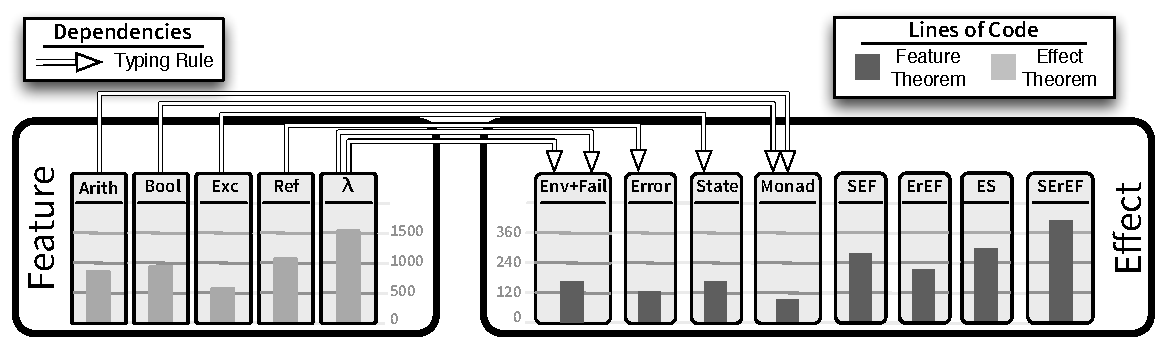
\includegraphics[scale = .85]{src/ModularEffects/CaseStudyFigure.pdf}
   }
  \end{center}
  \caption{Dependency and size information for the features and effects used in the case study.}
  \label{fig:codesize}
\end{figure*}

\section{Case Study}
\label{sec:CaseStudy}

As a demonstration of the \Name~framework, we have built a set of five
reusable language features and combined them to build a family of
languages which includes a mini-ML~\cite{clement86mini-ML} variant
with references and errors. The study includes pure boolean and
arithmetic features as well as effectful features for references,
errors and lambda abstractions.

The study builds twenty eight different combinations of the features which are
all possible combinations with at least one feature providing
values.\footnote{Also available at \url{http://www.cs.utexas.edu/~bendy/3MT}}
Figure~\ref{fig:MiniMLSyntax} presents the syntax of the expressions,
values, and types provided; each line is annotated with the feature
that provides that set of definitions.

Four kinds of feature interactions appear in the case study.

\begin{itemize}

\item The PHOAS representation of binders requires an auxiliary
equivalence relation, the details of which are covered in the MTC
paper~\cite{mtc}. The soundness proofs of language theorems for
languages which include binders proceed by induction over this
equivalence relation instead of expressions. The reusable feature
theorems of other features need to be lifted to this equivalence
relation.

\item The effect theorems that feature an environment
typing $\Sigma$, such as those for state or environment, need a weakening sublemma
which
states
that each well-formed value under
$\Sigma$ is also well-formed under a conservative extension:
\[\Sigma \vdash v ~:~ t  \\ \rightarrow \\
  \Sigma' \supseteq \Sigma \\ \rightarrow \\
  \Sigma' \vdash v ~:~ t \]
\item Inversion lemmas for the well-formed value relation as in the
proof of \ref{thm:FSound} for the boolean feature in
Section \ref{sec:Thm+Reuse} are proven by induction over the
relation.

%% \item The sublemmas of reusable feature theorems for properties such as
%% \textsc{WFM-If-Vc} are
%% proven by induction over the extensible typing relation. When effectful
%% features introduce new judgements to the relation, these new
%% judgements must have proof algebra instances for the sublemmas.

\end{itemize}


The proofs of the first and second kind of feature interactions are
straightforward; the inversion lemmas of the third kind can be
dispatched by tactics hooked into the type class inference algorithm.
%% The last kind of interactions require more work and comprise the
%% biggest part of the code dealing with feature interactions.
%%
%% The presented typing rules for effects satisfy the \textsc{WFM-Bind}
%% property; as previously discussed, it can be used cut down on feature
%% interactions. The lambda feature uses \textsc{WFM-Bind} in its proof
%% of \ref{thm:FSound} instead of targeted sublemmas. The following table
%% shows the number of sublemmas used by the reusable feature theorems,
%% highlighting that the \textsc{WFM-Bind} property provides significantly
%% more convenience despite its stronger assumptions.


The framework itself consists of about 4,400 LoC of which about 2,000
LoC comprise the implementation of the monad transformers and their
algebraic laws. The size in LoC of the implementation of semantic
evaluation and typing functions and the reusable feature theorem for
each language feature is given in the left box in Figure
\ref{fig:codesize}. The right box lists the sizes of the effect
theorems. Each language needs on average 110 LoC to assemble its
semantic functions and soundness proofs from those of its features and
the effect theorem for its set of effects.


\begin{figure}[t]
  \begin{center}
    \begin{minipage}{\columnwidth}
      \begin{center}
        \fbox{
        \hspace{-.3cm}
          \begin{tabular}{r@{~}c@{~}lr}
            {\tt e} & ::= & {\tt $\mathbb{N}$ $|$ e + e} & \textit{Arith}\\
            & $|$ &  {\tt $\mathbb{B}$ $|$ {\bf if} e {\bf then} e {\bf else} e} & \textit{Bool} \\
           %% & $|$ & {\tt {\bf case} e {\bf of \{ z} $\Rightarrow$ e $\mathbf{;}$ {\bf S} n $\Rightarrow$ e\}} & \textit{NatCase}\\
            & $|$ & {\tt {\bf lam} x : T.e $|$ e e $|$ x} & \textit{Lambda}\\
            & $|$ & {\tt {\bf ref} e $|$ !e $|$ e:=e} & \textit{References}\\
            & $|$ & {\tt {\bf try} e {\bf with} e} $|$ {\bf error} & \textit{Errors}\\
           %%  & $|$ & {\tt {\bf fix} x : T.e} & \textit{Recursion}\\
          \end{tabular}
        }
      \end{center}
    \end{minipage}
    \begin{minipage}{\columnwidth}
      \hspace{-.3cm}
    \begin{tabular}{cc}
      \begin{minipage}{.48\columnwidth}
        \fbox{
        \hspace{-.3cm}
          \begin{tabular}{r@{~}c@{~}lr}
            {\tt V} & ::= & {\tt $\mathbb{N}$} & \textit{Arith}\\
            & $|$ &  {\tt $\mathbb{B}$} & \textit{Bool} \\
            & $|$ & {\tt {\bf clos} e $\mathtt{\overline{V}}$} & \textit{Lambda}\\
            & $|$ & {\tt {\bf loc} $\mathbb{N}$} & \textit{References}\\
          \end{tabular}
        }
      \end{minipage} &
      \begin{minipage}{.38\columnwidth}
        \hspace{-.3cm}
        \fbox{
        \hspace{-.3cm}
          \begin{tabular}{r@{~}c@{~}lr}
            {\tt T} & ::= & {\tt \bf Nat} & \textit{Arith}\\
            & $|$ &  {\tt \bf Bool} & \textit{Bool} \\
            & $|$ & {\tt T $\rightarrow$ T} & \textit{Lambda}\\
            & $|$ & {\tt {\bf Ref} T} & \textit{References}\\
          \end{tabular}
        }
      \end{minipage}
    \end{tabular}
    \end{minipage}
  \end{center}
  \caption{mini-ML expressions, values, and types}
  \label{fig:MiniMLSyntax}
\end{figure}


%% \begin{center}
%%   \fbox{
%%   \hspace{-.3cm}
%%     \begin{tabular}{ c c c c c }
%%       \textit{Arith} & \textit{Bool} & \textit{Errors} & \textit{References} & \textit{Lambda} \\
%%       2 & 3 & 0 & 4 & 0 \\
%%     \end{tabular}
%%   }
%% \end{center}
%% Each sublemma of the above table requires on average 50 LoC per effect.

%% ODER: format ==         = "\mathrel{==}"
%% ODER: format /=         = "\neq "
%
%
\makeatletter
\@ifundefined{lhs2tex.lhs2tex.sty.read}%
  {\@namedef{lhs2tex.lhs2tex.sty.read}{}%
   \newcommand\SkipToFmtEnd{}%
   \newcommand\EndFmtInput{}%
   \long\def\SkipToFmtEnd#1\EndFmtInput{}%
  }\SkipToFmtEnd

\newcommand\ReadOnlyOnce[1]{\@ifundefined{#1}{\@namedef{#1}{}}\SkipToFmtEnd}
\usepackage{amstext}
\usepackage{amssymb}
\usepackage{stmaryrd}
\DeclareFontFamily{OT1}{cmtex}{}
\DeclareFontShape{OT1}{cmtex}{m}{n}
  {<5><6><7><8>cmtex8
   <9>cmtex9
   <10><10.95><12><14.4><17.28><20.74><24.88>cmtex10}{}
\DeclareFontShape{OT1}{cmtex}{m}{it}
  {<-> ssub * cmtt/m/it}{}
\newcommand{\texfamily}{\fontfamily{cmtex}\selectfont}
\DeclareFontShape{OT1}{cmtt}{bx}{n}
  {<5><6><7><8>cmtt8
   <9>cmbtt9
   <10><10.95><12><14.4><17.28><20.74><24.88>cmbtt10}{}
\DeclareFontShape{OT1}{cmtex}{bx}{n}
  {<-> ssub * cmtt/bx/n}{}
\newcommand{\tex}[1]{\text{\texfamily#1}}	% NEU

\newcommand{\Sp}{\hskip.33334em\relax}


\newcommand{\Conid}[1]{\mathit{#1}}
\newcommand{\Varid}[1]{\mathit{#1}}
\newcommand{\anonymous}{\kern0.06em \vbox{\hrule\@width.5em}}
\newcommand{\plus}{\mathbin{+\!\!\!+}}
\newcommand{\bind}{\mathbin{>\!\!\!>\mkern-6.7mu=}}
\newcommand{\rbind}{\mathbin{=\mkern-6.7mu<\!\!\!<}}% suggested by Neil Mitchell
\newcommand{\sequ}{\mathbin{>\!\!\!>}}
\renewcommand{\leq}{\leqslant}
\renewcommand{\geq}{\geqslant}
\usepackage{polytable}

%mathindent has to be defined
\@ifundefined{mathindent}%
  {\newdimen\mathindent\mathindent\leftmargini}%
  {}%

\def\resethooks{%
  \global\let\SaveRestoreHook\empty
  \global\let\ColumnHook\empty}
\newcommand*{\savecolumns}[1][default]%
  {\g@addto@macro\SaveRestoreHook{\savecolumns[#1]}}
\newcommand*{\restorecolumns}[1][default]%
  {\g@addto@macro\SaveRestoreHook{\restorecolumns[#1]}}
\newcommand*{\aligncolumn}[2]%
  {\g@addto@macro\ColumnHook{\column{#1}{#2}}}

\resethooks

\newcommand{\onelinecommentchars}{\quad-{}- }
\newcommand{\commentbeginchars}{\enskip\{-}
\newcommand{\commentendchars}{-\}\enskip}

\newcommand{\visiblecomments}{%
  \let\onelinecomment=\onelinecommentchars
  \let\commentbegin=\commentbeginchars
  \let\commentend=\commentendchars}

\newcommand{\invisiblecomments}{%
  \let\onelinecomment=\empty
  \let\commentbegin=\empty
  \let\commentend=\empty}

\visiblecomments

\newlength{\blanklineskip}
\setlength{\blanklineskip}{0.66084ex}

\newcommand{\hsindent}[1]{\quad}% default is fixed indentation
\let\hspre\empty
\let\hspost\empty
\newcommand{\NB}{\textbf{NB}}
\newcommand{\Todo}[1]{$\langle$\textbf{To do:}~#1$\rangle$}

\EndFmtInput
\makeatother
%
%
%
%
%
%
% This package provides two environments suitable to take the place
% of hscode, called "plainhscode" and "arrayhscode". 
%
% The plain environment surrounds each code block by vertical space,
% and it uses \abovedisplayskip and \belowdisplayskip to get spacing
% similar to formulas. Note that if these dimensions are changed,
% the spacing around displayed math formulas changes as well.
% All code is indented using \leftskip.
%
% Changed 19.08.2004 to reflect changes in colorcode. Should work with
% CodeGroup.sty.
%
\ReadOnlyOnce{polycode.fmt}%
\makeatletter

\newcommand{\hsnewpar}[1]%
  {{\parskip=0pt\parindent=0pt\par\vskip #1\noindent}}

% can be used, for instance, to redefine the code size, by setting the
% command to \small or something alike
\newcommand{\hscodestyle}{}

% The command \sethscode can be used to switch the code formatting
% behaviour by mapping the hscode environment in the subst directive
% to a new LaTeX environment.

\newcommand{\sethscode}[1]%
  {\expandafter\let\expandafter\hscode\csname #1\endcsname
   \expandafter\let\expandafter\endhscode\csname end#1\endcsname}

% "compatibility" mode restores the non-polycode.fmt layout.

\newenvironment{compathscode}%
  {\par\noindent
   \advance\leftskip\mathindent
   \hscodestyle
   \let\\=\@normalcr
   \let\hspre\(\let\hspost\)%
   \pboxed}%
  {\endpboxed\)%
   \par\noindent
   \ignorespacesafterend}

\newcommand{\compaths}{\sethscode{compathscode}}

% "plain" mode is the proposed default.
% It should now work with \centering.
% This required some changes. The old version
% is still available for reference as oldplainhscode.

\newenvironment{plainhscode}%
  {\hsnewpar\abovedisplayskip
   \advance\leftskip\mathindent
   \hscodestyle
   \let\hspre\(\let\hspost\)%
   \pboxed}%
  {\endpboxed%
   \hsnewpar\belowdisplayskip
   \ignorespacesafterend}

\newenvironment{oldplainhscode}%
  {\hsnewpar\abovedisplayskip
   \advance\leftskip\mathindent
   \hscodestyle
   \let\\=\@normalcr
   \(\pboxed}%
  {\endpboxed\)%
   \hsnewpar\belowdisplayskip
   \ignorespacesafterend}

% Here, we make plainhscode the default environment.

\newcommand{\plainhs}{\sethscode{plainhscode}}
\newcommand{\oldplainhs}{\sethscode{oldplainhscode}}
\plainhs

% The arrayhscode is like plain, but makes use of polytable's
% parray environment which disallows page breaks in code blocks.

\newenvironment{arrayhscode}%
  {\hsnewpar\abovedisplayskip
   \advance\leftskip\mathindent
   \hscodestyle
   \let\\=\@normalcr
   \(\parray}%
  {\endparray\)%
   \hsnewpar\belowdisplayskip
   \ignorespacesafterend}

\newcommand{\arrayhs}{\sethscode{arrayhscode}}

% The mathhscode environment also makes use of polytable's parray 
% environment. It is supposed to be used only inside math mode 
% (I used it to typeset the type rules in my thesis).

\newenvironment{mathhscode}%
  {\parray}{\endparray}

\newcommand{\mathhs}{\sethscode{mathhscode}}

% texths is similar to mathhs, but works in text mode.

\newenvironment{texthscode}%
  {\(\parray}{\endparray\)}

\newcommand{\texths}{\sethscode{texthscode}}

% The framed environment places code in a framed box.

\def\codeframewidth{\arrayrulewidth}
\RequirePackage{calc}

\newenvironment{framedhscode}%
  {\parskip=\abovedisplayskip\par\noindent
   \hscodestyle
   \arrayrulewidth=\codeframewidth
   \tabular{@{}|p{\linewidth-2\arraycolsep-2\arrayrulewidth-2pt}|@{}}%
   \hline\framedhslinecorrect\\{-1.5ex}%
   \let\endoflinesave=\\
   \let\\=\@normalcr
   \(\pboxed}%
  {\endpboxed\)%
   \framedhslinecorrect\endoflinesave{.5ex}\hline
   \endtabular
   \parskip=\belowdisplayskip\par\noindent
   \ignorespacesafterend}

\newcommand{\framedhslinecorrect}[2]%
  {#1[#2]}

\newcommand{\framedhs}{\sethscode{framedhscode}}

% The inlinehscode environment is an experimental environment
% that can be used to typeset displayed code inline.

\newenvironment{inlinehscode}%
  {\(\def\column##1##2{}%
   \let\>\undefined\let\<\undefined\let\\\undefined
   \newcommand\>[1][]{}\newcommand\<[1][]{}\newcommand\\[1][]{}%
   \def\fromto##1##2##3{##3}%
   \def\nextline{}}{\) }%

\newcommand{\inlinehs}{\sethscode{inlinehscode}}

% The joincode environment is a separate environment that
% can be used to surround and thereby connect multiple code
% blocks.

\newenvironment{joincode}%
  {\let\orighscode=\hscode
   \let\origendhscode=\endhscode
   \def\endhscode{\def\hscode{\endgroup\def\@currenvir{hscode}\\}\begingroup}
   %\let\SaveRestoreHook=\empty
   %\let\ColumnHook=\empty
   %\let\resethooks=\empty
   \orighscode\def\hscode{\endgroup\def\@currenvir{hscode}}}%
  {\origendhscode
   \global\let\hscode=\orighscode
   \global\let\endhscode=\origendhscode}%

\makeatother
\EndFmtInput
%
%
%
% First, let's redefine the forall, and the dot.
%
%
% This is made in such a way that after a forall, the next
% dot will be printed as a period, otherwise the formatting
% of `comp_` is used. By redefining `comp_`, as suitable
% composition operator can be chosen. Similarly, period_
% is used for the period.
%
\ReadOnlyOnce{forall.fmt}%
\makeatletter

% The HaskellResetHook is a list to which things can
% be added that reset the Haskell state to the beginning.
% This is to recover from states where the hacked intelligence
% is not sufficient.

\let\HaskellResetHook\empty
\newcommand*{\AtHaskellReset}[1]{%
  \g@addto@macro\HaskellResetHook{#1}}
\newcommand*{\HaskellReset}{\HaskellResetHook}

\global\let\hsforallread\empty

\newcommand\hsforall{\global\let\hsdot=\hsperiodonce}
\newcommand*\hsperiodonce[2]{#2\global\let\hsdot=\hscompose}
\newcommand*\hscompose[2]{#1}

\AtHaskellReset{\global\let\hsdot=\hscompose}

% In the beginning, we should reset Haskell once.
\HaskellReset

\makeatother
\EndFmtInput

% format runC         = "run\mathbb{C}_{\scalebox{0.6}{T}}"
% format C            = "\mathbb{C}_{\scalebox{0.6}{T}}"
%%format R            = "\mathbb{R}_{\scalebox{0.6}{T}}"


\section{Related and Future Work}

\paragraph{DGP in proof-assistants}

Datatype-generic programming started out as a form of language
extension such as PolyP \cite{jansson:polyp} or Generic Haskell
\cite{loh:dsgh}. Yet Haskell has turned out to be powerful enough to
implement datatype-generic programming in the language itself and over
the time a vast number of DGP libraries for Haskell have been proposed
\cite{cheney:ligd,syb,emgm,multirec,instantgenerics,uniplate,genericderiving}. Compared
with a language extension, a library is much easier to develop and
maintain.

Using the flexibility of dependent-types there are multiple proposals
for performing datatype-generic programming in proof assistants
\cite{dgpcoq,altenkirch:gpwdtp,benke:universes,loh:gpif,indexedcontainers}. This
setting not only allows the implementation of generic functions, but
also of generic proofs. The approaches vary in terms of how strictly
they follow the positivity or termination restrictions imposed by the
proof assistant. Some circumvent the type-checker at various points to
simplify the development or presentation while others put more effort
in convincing the type-checker and termination checker of the validity
\cite{ertt}. However, in all of the proposals there does not seem to
be any fundamental problem caused by the restrictions.


\paragraph{DGP for modular proofs}

Modularly composing semantics and proofs about the semantics has also
been addressed by \cite{schwaab:mtp} in the context of programming
language meta-theory. They perform their development in Agda and
similar to our approach they also use a universe approach based on
polynomial functors to represent modular datatypes. They split
relations for small-step operational semantics and well-typing on a
feature basis. However, the final fixed points are constructed manually
instead of having a generic representation of inductive families.

Using Coq's type classes both MTC and our approach also allow for more
automation in the final composition of datatypes, functions and
proofs. Agda features instance arguments that can be used to replace
type classes in various cases. However, the current implementation
does not perform recursive resolution and as a result Agda does not
support automation of the composition to the extent that is needed for
DTC-like approaches.


\paragraph{Combining different DGP approaches}

We have shown an embedding of the universe of polynomial functors into
the universe of containers. Similar inclusions between universes have
been done in the literature \cite{morris:cspf}. Magalh\~aes and L\"oh
\cite{jpm:fcadgp} have ported several popular DGP approaches from
Haskell to Agda and performed a formal comparison by proving inclusion
relations between the approaches.

DGP approaches differ in terms of the class of datatypes they capture and the
set of generic functions that can be implemented for them. Generic functions
can be transported from a universe into a sub-universe. However, we are not
aware of any DGP library with a systematic treatment of universes where each generic
function is defined on the most general universe that supports that function.


\paragraph{DGP for abstract syntax}

We have shown how to obtain more reuse by complementing modular
definitions with a generic equality function and generic proofs of its
properties. Of course more generic functionality like traversals,
pretty-printing, parsing etc. can be covered by means of
datatype-generic programming.

One very interesting idea is to use datatype-generic programming to
handle variable binding \cite{cheney:synp,unbound}. Variable
binding is an ubiquitous aspect of programming languages. Moreover, a
lot of functionality like variable substitutions and free variable
calculations is defined for many languages. Licata and Harper
\cite{licata:ubc} and Keuchel and Jeuring \cite{sk:gcasr} define
universes for datatypes with binding in Agda. Lee et al.~\cite{gmeta}
develop a framework for first-order representations of variable
binding in Coq that is based on the universe of regular tree types
\cite{ertt} and that provides many of the so-called
\emph{infrastructure lemmas} required when mechanizing programming
language meta-theory.

An interesting direction for future work is to extend these approaches
to capture variable binding in the indices of relations on abstract
syntax and use this as the underlying representation of extensible
datatypes and extensible logical relations and thereby complementing
modular functions with generic proofs about variable binding.


\paragraph{Automatic derivation of instances}

Most, if not all, generic programming libraries in Haskell use Template
Haskell to derive the generic representation of user-defined types and
to derive the conversion functions between them.

The GMeta \cite{gmeta} framework includes a standalone tool that also
performs this derivation for Coq. Similarly we also like to be able
to derive instances for the \ensuremath{\Conid{Container}} and \ensuremath{\Conid{Polynomial}} classes
automatically.


Formally mechanizing proofs can be very tedious and the amount of work
required for larger developments is excruciating. Meta-Theory \`a la Carte
is a framework for modular reusable components for use in
mechanizations. It builds on the Datatypes \`a la Carte approach to solve
an extended version of the expression problem. MTC allows modular
definitions of datatypes, semantic functions and logical relations and
furthermore modular inductive proofs.

MTC uses extensible Church-encodings to overcome conservative restrictions
imposed by the Coq proof-assistant. This approach has shortcomings
in terms of confidence in the definitions and in terms of usability. This
paper addresses these shortcomings by using datatype-generic
programming techniques to replace Church-encodings as the underlying representation
of type-level fixed points. Our approach avoids impredicativity, adequately
encodes fixed points and leads to stronger induction principles by
exploiting DGP approaches that capture only strictly-positive functors.

Working with generic structure representation has the added benefit that
we can implement generic functions like equality and generic proofs once and for all.



%%% Local Variables:
%%% mode: latex
%%% TeX-master: "../main"
%%% End:

}

\part*{Conclusion}
\addcontentsline{toc}{part}{Conclusion}

Formally mechanizing proofs can be very tedious and the amount of work
required for larger developments is excruciating. Meta-Theory \`a la Carte
is a framework for modular reusable components for use in
mechanizations. It builds on the Datatypes \`a la Carte approach to solve
an extended version of the expression problem. MTC allows modular
definitions of datatypes, semantic functions and logical relations and
furthermore modular inductive proofs.

MTC uses extensible Church-encodings to overcome conservative restrictions
imposed by the Coq proof-assistant. This approach has shortcomings
in terms of confidence in the definitions and in terms of usability. This
paper addresses these shortcomings by using datatype-generic
programming techniques to replace Church-encodings as the underlying representation
of type-level fixed points. Our approach avoids impredicativity, adequately
encodes fixed points and leads to stronger induction principles by
exploiting DGP approaches that capture only strictly-positive functors.

Working with generic structure representation has the added benefit that
we can implement generic functions like equality and generic proofs once and for all.


\appendix
\part*{Appendices}
\addcontentsline{toc}{part}{Appendices}
{
\newcommand{\ov}[1]{\overline{#1}}
\newcommand{\cpar}[1]{{\texttt{(}{#1}\texttt{)}}}
\newcommand{\cbrc}[1]{{\texttt{\{}{#1}\texttt{\}}}}
\newcommand{\cbrk}[1]{{\texttt{[}{#1}\texttt{]}}}
\newcommand{\ccol}{\texttt{:}}
\newcommand{\cass}{\texttt{:=}}
\newcommand{\cto}{~\texttt{->}~}

\newcommand{\fieldref}[2]{\cpar{{#1}\,\texttt{@}\,{#2}}}
\newcommand{\fieldbind}[2]{\cpar{{#1}\,\ccol\,{#2}}}
\newcommand{\fieldsub}[2]{\cpar{{#1}\,\ccol\,{#2}}}
\newcommand{\evalbs}[2]{{\llbracket\:{#1}\:\rrbracket_{#2}}}
\newcommand{\evalbig}[3]{[{#1}] {#2} \Downarrow {#3}}
\newcommand{\evalbigf}[3]{{#1}({#2}) \Downarrow {#3}}
\newcommand{\evalsym}[3]{{\llbracket\: {#1} \mid {#2} \:\rrbracket_{#3}}}
\newcommand{\evalrbs}[4]{{\llbracket\: {#1} \:\rrbracket_{{#3},{#4}}}}
\newcommand{\symflatten}[3]{{{#1} \vdash_E {#2} \Downarrow {#3}}}

\newcommand{\typing}[3]{{#1} \vdash_\text{tm} {#2} : {#3}}

\newcommand{\fprod}{\ensuremath{F_\times}\xspace}
\newcommand{\POPLmark}{\textsc{POPLmark}\xspace}
\newcommand{\LNGen}{\textsc{LNGen}\xspace}
\newcommand{\DbGen}{\textsc{DbGen}\xspace}
\newcommand{\Ott}{\textsc{Ott}\xspace}
\newcommand{\Romeo}{\textsc{Romeo}\xspace}
\newcommand{\AutoSubst}{\textsc{AutoSubst}\xspace}
\newcommand{\GMeta}{\textsc{GMeta}\xspace}
\newcommand{\SystemF}{System~F\xspace}
\newcommand{\SystemFsub}{\ensuremath{\text{System~F}_{<:}}\xspace}
\newcommand{\LF}{\textlambda LF\xspace}
\newcommand{\CoC}{\textsc{CoC}\xspace}
\newcommand{\stlc}{\ensuremath{\lambda}\xspace}
\newcommand{\stlcprod}{\ensuremath{\lambda_{\times}}\xspace}
\newcommand{\F}{\ensuremath{F}\xspace}
\newcommand{\fsub}{\ensuremath{F_{<:}}}
\newcommand{\fsubprod}{\ensuremath{F_{<:,\times}}}
\newcommand{\Unbound}{\textsc{Unbound}\xspace}
\newcommand{\lomega}{\ensuremath{\lambda_{\omega}}\xspace}
\newcommand{\fomega}{\ensuremath{F_{\omega}}\xspace}
\newcommand{\fseqlet}{\ensuremath{F_\text{seq}}}
\newcommand{\fsubrcd}{\ensuremath{F_{<:,\text{rcd}}}}
\newcommand{\fexists}{\ensuremath{F_{\exists}}\xspace}
\newcommand{\fexistsprod}{\ensuremath{F_{\exists,\times}}\xspace}

\newcommand{\spec}{\mathit{spec}}
\newcommand{\decl}{\mathit{decl}}
\newcommand{\namedecl}{\mathit{namedecl}}

\newcommand{\knotkeyword}[1]{{\texttt{#1}}}
\newcommand{\namespace}{\knotkeyword{namespace}}
\newcommand{\sort}{\knotkeyword{sort}}
\newcommand{\function}{\knotkeyword{fun}}
\newcommand{\env}{\knotkeyword{env}}
\newcommand{\relation}{\knotkeyword{relation}}
\newcommand{\subst}{\knotkeyword{subst}}
\newcommand{\In}{\knotkeyword{In}}

\newcommand{\sortdecl}{\mathit{sortdecl}}
\newcommand{\condecl}{\mathit{condecl}}
\newcommand{\bsi}{\mathit{bsi}}
\newcommand{\bindspec}{\mathit{bs}}
\newcommand{\fundecl}{\mathit{fundecl}}
\newcommand{\funclause}{\mathit{funclause}}

\newcommand{\envdecl}{\mathit{envdecl}}
\newcommand{\envclause}{\mathit{envclause}}
\newcommand{\reldecl}{\mathit{reldecl}}
\newcommand{\ruledecl}{\mathit{ruledecl}}
\newcommand{\formula}{\mathit{fml}}
\newcommand{\lookup}{\mathit{lookup}}
\newcommand{\jmv}{\mathit{j}}
\newcommand{\judgement}{\mathit{jmt}}
\newcommand{\rulebindspec}{\mathit{rbs}}
\newcommand{\rbsi}{\mathit{rbsi}}
\newcommand{\symbolicterm}{\mathit{sym}}
\newcommand{\symboliccoterm}{\mathit{cosym}}
\newcommand{\symbolicweaken}{\mathbf{weaken}}
\newcommand{\symboliccoweaken}{\mathbf{coweaken}}
\newcommand{\symbolicsubst}{\mathbf{subst}}
\newcommand{\symbolicenv}{\theta}
\newcommand{\LENV}{\mathcal{L}}
\newcommand{\VENV}{\mathcal{V}}
\newcommand{\RENV}{\mathcal{R}}
\newcommand{\dom}{\text{dom}}
\newcommand{\domain}[1]{{\dom~{#1}}}

\newcommand{\wfbindspec}[3]{\LENV; {#1} \vdash {#2}}  %  : {#3}
\newcommand{\wfsym}[3]{\LENV; {#1} \vdash {#2} : {#3}}
\newcommand{\wfruledecl}[4]{\vdash_{#1,#2,#3} #4}
\newcommand{\wfformula}[2]{\LENV \vdash_{#1} {#2}}

\newcommand{\judg}[4]{{#1} \models_{#2} {#3} ; {#4}}
\newcommand{\judgsimpl}[3]{{#1} \models_{#2} {#3}}
\newcommand{\lookupenv}[5]{{ ({#1}:{#2}) \in_{{#3},{#4}} {#5}}}

\newcommand{\eqtreflcon}{\text{qrf}}
\newcommand{\eqttranscon}{\text{qtr}}
\newcommand{\eqtsymcon}{\text{qsm}}
\newcommand{\eqtregcon}{\text{qcn}}

\newcommand{\Eqh}[4]{\models_{#1} {#2} : {#3} \equiv {#4}}
\newcommand{\Equ}[6]{{#1} \equiv {#2} \models_{#3} {#4} : {#5} \equiv {#6}}

\newcommand{\eqt}{\text{eqt}}
\newcommand{\eqtrefl}[3]{\eqtreflcon~{#1}~{#2}~{#3}}
\newcommand{\eqttrans}[2]{\eqttranscon~{#1}~{#2}}
\newcommand{\eqtsym}[1]{\eqtsymcon~{#1}}
\newcommand{\eqtreg}[2]{\eqtregcon~{#1}~{#2}}
\newcommand{\sh}[3]{\text{sh}_{#1}~{#2}~{#3}}
\newcommand{\su}[4]{\text{su}_{#1}~{#2}~{#3}~{#4}}
\newcommand{\shstar}{{\text{sh}^{*}}}
\newcommand{\wk}[2]{\shstar~{#1}~{#2}}
\newcommand{\eqtshiftweaken}[2]{\text{qhw}~{#1}~{#2}}
\newcommand{\eqtshiftsubst}[2]{\text{qhu}~{#1}~{#2}}
\newcommand{\eqtsubstweaken}[1]{\text{quw}~{#1}}
\newcommand{\eqtsubstsubst}[1]{\text{quu}~{#1}}
\newcommand{\eqtcongweaken}[2]{\text{qcw}~{#1}~{#2}}
%% \newcommand{\eqterm}[8]{\LENV;{#1};{#2};{#3} \models {#4} : ({#5} \vdash {#6} = {#7} : {#8})}
\newcommand{\eqterm}[8]{{#4} \models_{\LENV,{#1},{#2},{#3}} ({#5} \vdash {#6} = {#7} : {#8})}
\newcommand{\knotbox}[1]{{\hspace{-1em}\framebox{\mbox{\ensuremath{#1}}}}}

\newcommand{\wsterm}[7]{({#3}) \models_{#5} ({#4} \vdash_{#7} {#6})}
\newcommand{\wnindex}[7]{({#3}) \models_{#5} ({#4} \vdash_{#7} {#6})}

\newcommand{\igfunclause}[2]{ #1 \equiv #2 \\}
\newcommand{\ignt}[1]{\mathit{#1}}
\newcommand{\igmv}[1]{\mathit{#1}}
\newcommand{\igkw}[1]{\mathbf{#1}}
\newcommand{\igsym}[1]{#1}
\newcommand{\igcom}[1]{\text{#1}}
\newcommand{\igdrulename}[1]{\textsc{#1}}
\newcommand{\igcomplu}[5]{\overline{#1}^{\,#2\in #3 #4 #5}}
\newcommand{\igcompu}[3]{\overline{#1}^{\,#2<#3}}
\newcommand{\igcomp}[2]{\overline{#1}^{\,#2}}

%%% Local Variables:
%%% mode: latex
%%% TeX-master: "Main"
%%% End:

\input{src/GenBinding/AppendixSpecification}
%% \input{src/GenBinding/AppendixSemantics}
\input{src/GenBinding/AppendixElaboration}
}

\backmatter



% Bibliography settings
\bibliographystyle{apalike}
% Keeping stuff in separate bibliography files is not convenient, as we often have duplicate entries.
\bibliography{Bibliography}


% Fix hyperref displaying/jumping to wrong page number for index: that of the list of tables.
% See http://tex.stackexchange.com/questions/138903/wrong-hyperref-for-index-in-tableofcontents-since-texlive-2010
% It now does not jump exactly to the title, but at least to the first index entry.
\clearpage
\phantomsection
% Index, this is the very last thing in Michaels thesis book.
\printindex

\end{document}
